% Complete Global Economy notes
% Set up for pdflatex

% sets formatting parameters etc
\documentclass[8pt,twoside,pdftex]{book}

% nice book overview: http://www.math.mun.ca/~edgar/thesis.html
% see esp indexing w/ package makeidx
% more at:  http://en.wikibooks.org/wiki/LaTeX/Indexing

% link colors etc:  black for Amazon, blue for the online version
\usepackage[colorlinks=true,
            allcolors=blue,
%            linkcolor=black,
%            citecolor=black,
%            urlcolor=blue,
            bookmarks=true,
            pdfstartview={FitV},
            pdftitle={The Global Economy},
            pdfsubject={A course in macroeconomics for business students},
            pdfauthor={The NYU Stern Economics Team}
            ]{hyperref}

\usepackage{amsmath, amssymb, amsthm}
\usepackage{graphicx}
\usepackage{color}
\usepackage{comment}
\usepackage{layout}
\usepackage{booktabs}

%Clean up the compiler output, so it is easier to find real problems.
\hbadness = 12000                %Loosen under/overfull box warning
\hfuzz = 5.0pt                  %No overfill warning is less than 5pt overhang
\pdfoptionpdfminorversion 6     %Kill off warning  about pdf version

% list spacing
\usepackage{enumitem}
\setitemize{leftmargin=*, topsep=0pt, partopsep=0pt}
\setenumerate{leftmargin=*, topsep=0pt, partopsep=0pt}

% set paths for graphics and tables
% http://kawahara.ca/latex-how-to-programmatically-change-the-path-of-your-figures/
% http://stackoverflow.com/questions/1211888/is-there-any-way-i-can-define-a-variable-in-latex
\newcommand{\figpath}{../}
\newcommand{\tabpath}{../}
\newcommand{\blurbpath}{../}

\usepackage{caption}
\usepackage{setspace}
\usepackage{float}

% for index
\usepackage{makeidx}
\usepackage[indentunit=2.0em, justific=RaggedRight, columnsep=2.5em]{idxlayout}

%Turn off ligatures to make pdf searchable, turn on ligatures to make font pretty
\usepackage{microtype}
\DisableLigatures{encoding = *, family = * }

% Adjust fonts for chapter and section headings
% old version
\usepackage[medium, compact]{titlesec}
\titleformat{\section}{\large\bfseries\sffamily}{\thesection\sffamily}{1em}{}
\titleformat{\subsection}{\normalsize\bfseries\sffamily}{\thesection}{1em}{}
\titleformat{\part}{\bfseries\huge\sffamily}{}{0pt}{Part \thepart\\}  % edited by LC
\titleformat{\chapter}{\bfseries\huge\sffamily}{}{0pt}
        {\ifnum\thechapter>0\resizebox{!}{25pt}{\thechapter}\\ \fi}
%This handles the chapters that are not numbered, such as long-term overview and preface.
\titleformat{name=\chapter,numberless}{\bfseries\huge\sffamily}{\sffamily}{0em}{}




% LC  version
%\usepackage[medium, compact, sf, bf]{titlesec}
%\titleformat{\section}{\large\bfseries\sffamily}{\thesection}{1em}{}
%\titleformat{\subsection}{\normalsize\bfseries\sffamily}{\thesection}{1em}{}
%\titleformat{\part}{\bfseries\huge\sffamily\uppercase}{}{0pt}{Part \thepart\\}
%\titleformat{\chapter}{\bfseries\huge\sffamily\uppercase}{}{0pt}
%        {\ifnum\thechapter>0\resizebox{!}{30pt}{\thechapter}\\ \fi}

% to kill off awkward pagebreaks -- manually
\usepackage{needspace}
% example:  \needspace{4\baselineskip} makes sure we have four lines available before pagebreak

% for left spacing of problems, summary, etc
% no longer used
\newlength{\oldleftmargini}
\setlength{\oldleftmargini}{\leftmargini}

% for spacing of table of contents
% see http://tex.stackexchange.com/questions/49877/table-of-contents-spacing
% problem:  messes up spacing and fonts of table and figure lists in toc, so killed them off
\usepackage{tocloft}
\renewcommand\cftchapafterpnum{\vskip3pt}
\renewcommand{\cftchapfont}{\sffamily \large}               %San serif font for chapter headings
\renewcommand{\cftpartfont}{\sffamily \Large}               %San serif font for part headings
\renewcommand{\cftsecfont}{\sffamily}               %San serif font for part headings

%%%%%%%%%%%%%%%%%%%%%%Margins%%%%%%%%%%%%%%%%%%%%%%%%%%%%%%%%%%%%%%%%%%%%%%%
% http://en.wikibooks.org/wiki/LaTeX/Page_Layout
\usepackage{geometry}
\geometry{paperwidth=6in, paperheight=9in, outer=0.6in, inner=0.85in, bottom=0.6in}
%\usepackage[cam,letter,center,pdftex]{crop}

% indentation and para skips
\setlength{\parindent}{0in}
\setlength{\parskip}{\bigskipamount}  % this is diddled further in the front_matter
\raggedbottom

%%%%%%%%%%%%%%%%%%%%Tighten up the lists%%%%%%%%%%%%%%%%%%%%%%%%%%%%%%%%%%%
% ?? made obsolete by enumitem?
\let\OLDdescription\description
\renewcommand\description{\OLDdescription\setlength{\itemsep}{-2mm}}

%%%%%%%%%%%%%%%%%%%%%%Headers and Footers%%%%%%%%%%%%%%%%%%%%%%%%%%%%%%%%%%
\usepackage{fancyhdr}
\pagestyle{fancy}
\fancyhead{}
\fancyfoot{}
\renewcommand{\chaptermark}[1]{\markboth{\thechapter.\ #1}{}}
\fancyhead[RO]{\leftmark \hspace{0.25in} \thepage}
\fancyhead[RE]{}
\fancyhead[LE]{\thepage \hfill Global Economy @ NYU Stern}

%%%%%%%%%%%%%%%%%%%%%%Special Characters%%%%%%%%%%%%%%%%%%%%%%%%%%%%%%%%%%%%
\newcommand{\GDP}{\mbox{\em GDP\/}}
\newcommand{\NDP}{\mbox{\em NDP\/}}
\newcommand{\GNP}{\mbox{\em GNP\/}}
\newcommand{\NX}{\mbox{\em NX\/}}
\newcommand{\NY}{\mbox{\em NY\/}}
\newcommand{\CA}{\mbox{\em CA\/}}
\newcommand{\NFA}{\mbox{\em NFA\/}}

\newcommand{\Def}{\mbox{\em Def\/}}
\newcommand{\DS}{\mbox{\em DS\/}}
\newcommand{\CPI}{\mbox{\em CPI\/}}
\newcommand{\POP}{\mbox{\em POP\/}}
\newcommand{\CU}{\mbox{\em CU\/}}
\newcommand{\RE}{\mbox{\em RE\/}}
\newcommand{\MB}{\mbox{\em MB\/}}
\newcommand{\MONE}{\mbox{\em M1\/}}
\newcommand{\MTWO}{\mbox{\em M2\/}}
\newcommand{\IP}{\mbox{\em IP\/}}
\newcommand{\RER}{\mbox{\em RER\/}}

%%%%%%%%%%%%%%%%%%%%%%%%%%%%Load Indexing Commands%%%%%%%%%%%%%%%%%%%%%%%%%%%%%%%
\makeindex




%%%%%%%%%%%%%%%%%%%%%%%%%%%%%%%%%%%%%%%%%%%%%%%%%%%%%%%%%%%%%%%%%%%%%%%%%%%%%%%%%%%%%%%%%%%%%%%%%%%%
%To create a single chapter with the correct page numbering and references:                        %
%This isn't elegant, if you know a better way to do this, tell me.                                 %
%                                                                                                  %
% 1.  Go into preamble and set bookmarks=false.                                                    %
% 2.  Compile the entire book                                                                      %
% 3.  Uncomment the appropriate "includeonly" statement.                                           %
% 4.  The pdf will still be called "The_Global_Economy," so save it with the right filename.       %
% 5.  Some chapters may have a blank page at the beginning.  Use Acrobat to delete it.             %
%                                                                                                  %
%\includeonly{a_notes_front_matter}                                                                %
%\includeonly{notes_math}                                                                          %
%\includeonly{notes_data}                                                                          %
%\includeonly{notes_review_long}                                                                   %
%\includeonly{notes_production}                                                                    %
%\includeonly{notes_solow}                                                                         %
%\includeonly{notes_growth}                                                                        %
%\includeonly{notes_institutions}                                                                  %
%\includeonly{notes_finance}                                                                       %
%\includeonly{notes_trade}                                                                         %
%\includeonly{notes_labor}                                                                         %
%\includeonly{notes_review_short}                                                                  %
%\includeonly{notes_cycles}                                                                        %
%\includeonly{notes_indicators}                                                                    %
%\includeonly{notes_inflation}                                                                     %
%\includeonly{notes_asad}                                                                          %
%\includeonly{notes_asadpolicy}                                                                    %
%\includeonly{notes_monpol}                                                                        %
%\includeonly{notes_taxes}                                                                         %
%\includeonly{notes_deficits}                                                                      %
%\includeonly{notes_bop}                                                                           %
%\includeonly{notes_fx}                                                                            %
%\includeonly{notes_fxregimes}                                                                     %
%\includeonly{notes_crises}                                                                        %
%%%%%%%%%%%%%%%%%%%%%%%%%%%%%%%%%%%%%%%%%%%%%%%%%%%%%%%%%%%%%%%%%%%%%%%%%%%%%%%%%%%%%%%%%%%%%%%%%%%%


\begin{document}

%Title page, tables of contents, figures, etc.
\frontmatter
%%%%%%%%%%%%%%%%%%%%%%%%%%%%%%%%%%%%%%%%%%%%%%%%%%%%%%%%%Front Matter%%%%%%%%%%%%%%%%%%%%%%%%%%%%%%%%%%%%%%%
\begin{titlepage}
%\pagenumbering{roman}

\begin{center}
\textsc{}\\[1.5in]
{\Huge\bf The Global Economy} \\ [0.5in]
\end{center}

\pagebreak
\phantom{x}
\thispagestyle{empty}

\pagebreak
\thispagestyle{empty}
\begin{center}
\textsc{}\\[1.5in]
{\Huge\bf The Global Economy} \\ [0.25in]
{\huge\bf Version 2.1}

\vspace*{1.00in}
{\huge\bf NYU Stern Economics}

\vfill
{
\includegraphics[width=0.65\textwidth]{\figpath Figures/stern_black1.png}\\
%\textsc{\large Department of Economics}\\
[1.5in]
}
\end{center}


%%%%%%%%%%%%%%%%%%%%%%%%%%%%%%%%%%%%%%%%%%%%%%%%%%%%%%%%%%%%%%%%%%%%%%%%%%%%%%%%%%%%%%%%%%%%%%%%%%%%%%%
\newpage
\thispagestyle{empty}
\phantom{x}
\vfill
This document was created for the Global Economy course at New York
University's Stern School of Business by a team that includes
Dave Backus, Gian Luca Clementi, Tom Cooley, Joe Foudy, Kim Ruhl,
Kim Schoenholtz, Laura Veldkamp, Venky Venkateswaran, Paul Wachtel, Mike Waugh,
and Stan Zin.
The cover was designed by Alexa Zin.
The most recent version of this document, and related materials,
will be posted at

\vspace*{\parskip}
\centerline{\url{http://www.stern.nyu.edu/GEMatter}.}

%\vspace{0.15 in}
This version was created \today.

%\vspace{\parskip}
Copyright \copyright \ \number\year \ by New York University's Center for Global Economy and Business

\begin{minipage}{0.9in}
\begin{flushleft}
\vspace{0.12in}

\includegraphics[width=0.9in]{\figpath Figures/by_sa.pdf} \\
\vfill
\vspace{0.27in}
\phantom{m}
\end{flushleft}
\end{minipage}
\hspace{0.1in}
%
\begin{minipage}{0.80\textwidth}
\begin{flushleft}
 This work is licensed under the Creative Commons Attribution-ShareAlike 3.0 Unported License.\\
 \vspace{0.05in}
 To view a copy of this license, visit \\ \url{http://creativecommons.org/licenses/by-sa/3.0/}.\\
 \end{flushleft}
\end{minipage}
\end{titlepage}

% Table of contents
% check this out re spacing after ch title
% http://tex.stackexchange.com/questions/33982/paragraph-spacing-affecting-table-of-contents?rq=1

% reduce spacing in toc
\parskip = 0.0\bigskipamount
\tableofcontents
%\addcontentsline{toc}{chapter}{Contents} % circular?
%\listoffigures
%\addcontentsline{toc}{chapter}{List of Figures}
%\listoftables
%\addcontentsline{toc}{chapter}{List of Tables}

\chapter*{Preface}
\addcontentsline{toc}{chapter}{Preface}
% put full spacing back
\parskip = \bigskipamount

This document evolved from a set of notes developed
for the Global Economy course at New York
University's Stern School of Business.
The idea behind the course is to use the tools of macroeconomics
to assess the economic performance of countries
and the challenges facing businesses operating in them.
We emphasize data;
virtually every chapter includes links to useful data sources.
The book is designed as background reading for the in-class experience.
It focuses on tools,
leaving us to spend most of our class time on applications.

We have posted all of our materials online
and offer them to others with similar interests in the hope
that they will reciprocate.
``We'' here means the Global Economy team:
Dave Backus, Gian Luca Clementi, Tom Cooley, Joe Foudy, Kim Ruhl, Kim Schoenholtz,
Laura Veldkamp, Venky Venkateswaran, Paul Wachtel, Mike Waugh, and Stan Zin.
This set of notes is available online
through the
\href{http://www.stern.nyu.edu/experience-stern/about/departments-centers-initiatives/centers-of-research/global-economy-business/index.htm}
{Center for Global Economy and Business}
at

\vspace*{\parskip}
\centerline{\url{http://www.stern.nyu.edu/GEMatter}.}

The same site includes the Stata files used to generate figures and tables.
The online version of the notes includes color graphs
and an extensive collection of links.
We offer an inexpensive black-and-white printed version through Amazon,
self-published through their CreateSpace facility,
which we were delighted with.
%(search ``amazon self-publish'').

Additional materials are available to those who ask nicely.
That includes slides (some of us use Beamer, but most use Powerpoint),
problem sets, exams, and R code for a variety of data sources.
We're equally interested in your thoughts:  on the course,
the materials, teaching macroeconomics, or anything else that crosses
your mind.
Send us an email, we're easy to track down.

One last request:  Please pass on any typos or other glitches you find.
Your efforts will help us improve future versions.

% Add thanks ...


% I think if we added \mainmatter [??] here, roman numerals would be auto
\mainmatter
% Preliminaries
\part{Preliminaries}
%\thispagestyle{empty}  %  useless 

%\textbf{Measurement}
%\begin{itemize}
%\item GDP is value added, payments to labor and capital, and expenditure. These three measurement are linked through accounting identities.
%\item Current price variables (like nominal GDP) can be decomposed into price changes and quantity (real) changes. The two methods to decompose current price variables into changes in prices and quantities are fixed price and fixed basket price indexes.
%\item GDP tells us a lot about an economy; price indexes are useful, but not without problems
%\end{itemize}

\chapter{Mathematics Review}\label{chp:math}
\hypertarget{math}{}

%No extra line here.
\textbf{Tools:} Exponents and logarithms; growth rates and compounding; derivatives; spreadsheets; the FRED database.

\textbf{Key Words:} Production function; demand function; 
marginal product\index{capital!marginal product of}; marginal cost.

\textbf{Big Ideas:}
%\vspace{-0.1in}
\begin{itemize}
    \item  Macroeconomics is a quantitative discipline; ditto business.
    \item  Mathematics and data analysis are essential tools.
\end{itemize}

\rule{\textwidth}{1pt}

Mathematics is a precise and efficient language for expressing quantitative ideas,
including many that come up in business.
%You can live without it, but you'll make some aspects of your life easier if you bite the bullet
%and teach yourself the most important aspects of mathematics.
What follows is an executive summary of everything you'll need in this course:
functions, exponents and logarithms, derivatives, and spreadsheets,
each illustrated with examples.


\section{Functions}

In economics and business, we often talk about relations between
variables: Demand depends on price; cost depends on quantity
produced; price depends on yield\index{bond!bond yield}; output depends on input; and so
on. We call these relations {\it functions\/}. \index{function} More formally, a
function $f$ assigns a (single) value $y$ to each possible value
of a variable $x$.
%For now, you should think of $x$ as a single variable, but later on
%we'll consider situations in which $x$ may stand for several
%different variables.
We write it this way: $y = f(x)$. Perhaps the
easiest way to think about a function is to draw it: Put $x$ on
the horizontal axis and plot the values of $y$ associated with
each $x$ on the vertical axis. In a spreadsheet program, you might
imagine setting up a table with a grid of values for $x$. The
function would then be a formula that computes a value $y$ for
each value of $x$.

%We will generally be interested in functions that are ``continuous'' (they don't have jumps)
%and ``smooth'' (they don't have kinks, either).


\textbf{Example:} Demand functions. \index{demand function}
We may be interested in the sensitivity of demand for our product to its price.
If the quantity demanded is $q$ and the price $p$,
an example of a  demand function relating the two is
\[
    q \;=\; a + b p ,
\]
where $a$ and $b$ are ``parameters''
(think of them as fixed numbers whose values we haven't bothered to write down).
Sensitivity of demand to price is summarized by $b$,
which we'd expect to be negative (demand falls as price rises).


\textbf{Example:} Production functions. \index{production function}
In this class, we'll relate output $Y$ to inputs of capital $K$ and labor $L$.
(In macroeconomics, capital refers to plant and equipment.)
It'll look a little strange the first time you see it,
but a convenient example of such a function is
\[
    Y \;=\; K^\alpha L^{1-\alpha} ,
\]
where $\alpha$ is a number between zero and one (typically, we set $\alpha = 1/3$).
This is a modest extension of our definition of a function---$Y$ depends on two variables, not one---but the idea is the same.

\textbf{Example:} Bond yields\index{bond!bond yield}. \index{bond}
The price $p$ and yield \index{bond!bond yield}
 $y$ for a one-year zero-coupon bond \index{bond}
might be related by
\[
    p \;=\; \frac{100}{1+y},
\]
where 100 is the face value of the bond. \index{bond}
Note the characteristic inverse relation:  high yield\index{bond!bond yield|textbf}, low price.


\section{Exponents and logarithms}

Exponents and logarithms are useful in many situations:
elasticities, compound interest, growth rates, and so on.
Here's a quick summary.

\textbf{Exponents.} Exponents are an extension of multiplication.
If we multiply $x$ by itself, we can write either $ x \times x $ or $x^2$,
where $2$ is an exponent (or power).
In general, we can write $x^a$ to mean (roughly) ``$x$ multiplied by itself $a$ times,''
although this language may seem a little strange
if $a$ isn't a positive whole number such as 2 or 3.
We can, nevertheless, compute such quantities for any value of $a$ we like
as long as $x$ is positive.
(Think about how you'd do this in a spreadsheet.)


The most useful properties of exponents are
\begin{eqnarray*}
    x^a x^b &=& x^{a+b} \\
    x^a y^a &=& (xy)^a \\
    (x^a)^b &=& x^{ab} \\
    x^{-a} &=& {1}/{x^a}.
\end{eqnarray*}
You can work these out for yourself using our multiplication analogy.


\textbf{Logarithms.}
By logarithm\index{logarithm}, we mean the function ``LN'' in
Microsoft Excel, OpenOffice Calc, or Google spreadsheets,
sometimes called the \textit{natural logarithm}.
%We write ``logarithm'' in these notes to represent the natural logarithm because that is how you will find it in most 5publications.


The natural logarithm of a number $x$ comes from the power of a number $e$,
a mathematical constant that is approximately 2.718.
If $x = e^y$, then $y$ is the logarithm of $x$,
expressed $y = \ln x $.
There are other logarithms based on powers of other numbers,
but we'll stick with $e$.
Some people use $\log$ to mean $\ln$, but that's a story for another time.
%The calculator or Excel function to obtain a natural logarithm is ``LN'' rather than ``LOG'' (which calculates a logarithm for base 10 rather than base $e$).
In this class, including assignments and exams, we \emph{always} use $\ln$ and LN,
not $\log$ or LOG.


Suppose that you know that $y$ is the logarithm of $x$.
How do you find $x$?  From the definition, apparently $x = e^y$.
In Excel, this is written ``$\exp(y)$.''
As a check, you might verify that $ \ln 6 = 1.792$ and $\exp(1.792) = 6.00$.


The most useful properties of logarithms
 are:
\begin{eqnarray*}
    \ln (xy) &=& \ln x + \ln y  \\
    \ln (x/y) &=& \ln x - \ln y    \\
    \ln (x^a) &=& a \ln x  \\
    \ln (\exp(x)) &=& x \\
    \exp(\ln x) &=& x \\
    \ln (1 + x) &\approx& x, \ \ \mbox{when \ $x$ \ is small}.
\end{eqnarray*}
The wiggly equals sign means ``approximately equal to.''
That's true for the last equation when $x$ is close enough to zero:
a number like 0.1 rather than 0.9 or 1.2 or 10.
In short, logarithms convert multiplication into addition, division into subtraction,
and ``exponentiation'' into multiplication. In each case, an operation is converted into a simpler one:
Addition, for example, is simpler than multiplication.


\textbf{Example:} Demand functions.
A more useful demand function is $ q = a p^b $,
which is linear in logarithms:
\[
    \ln q \;=\; \ln a + b \ln p .
\]
This follows from the first and third properties of logarithms.
Here, $b$ is the price elasticity you may have learned about in a microeconomics class.

\textbf{Example:} Production functions.
Understanding differences  in output per worker (across production units, firms, countries) is a central question in macroeconomics and this course. Using the production function discussed above, we can use properties of exponents to arrive at an expression suitable for this analysis. Using the production function
\begin{eqnarray*}
    Y = K^{\alpha} L^{1-\alpha},
\end{eqnarray*}
use the first and last property of exponents to obtain
\begin{eqnarray*}
    Y &=& K^{\alpha} L L^{-\alpha} \\
      &=& K^{\alpha} L ({1}/{L^{\alpha}}).
\end{eqnarray*}
Combining the terms with the $\alpha$ exponent and then using the second property of exponents, we have
\begin{eqnarray*}
     Y &=& \left( {K}/{L} \right)^{\alpha} L.
\end{eqnarray*}
Finally, dividing both sides by $L$ leaves us with the expression
\begin{eqnarray*}
     {Y}/{L} &=& \left( {K}/{L} \right)^{\alpha}.
\end{eqnarray*}
In words, output per worker equals capital per worker to the exponent $\alpha$.
%\begin{eqnarray*}
%    \ln Y = \alpha \ln K L^{1-\alpha}.
%\end{eqnarray*}

\section{Growth rates}
\label{sec:growth_math}

Growth rates\index{growth rate}
 are frequently used in this class, in the business world, and in life in general.
%We explain how to calculate and interpret them,
%focusing on two types.
We will use two types --- sorry, it can't be avoided.
The first is a \emph{discretely-compounded growth rate}.\index{growth rate!discretely compounded}
For a time interval of one year, this is analogous to an annually-compounded interest rate.
The second is a {\it continuously-compounded   growth rate\/}.
This is analogous to a continuously-compounded   interest rate,
in which interest is compounded over a very short time interval.
The former is more natural is some respects,
but the latter leads to simpler expressions when compounding is important.
%We'll use both.

\subsection*{Discretely-compounded growth rates\index{growth rate!discretely compounded}}

The simplest growth rates are those that are compounded each period $t$ at discrete time intervals. If the time period is a year (which will frequently be the case), then this corresponds with annual compounding\index{annual compounding}. The annually compounded growth rate relates variable $x$ across time periods as
\begin{eqnarray*}
x_{t+1} = (1 + g)x_{t},
\end{eqnarray*}
where lower case $g$ will denote the discretely-compounded\index{growth rate!discretely compounded} growth rate.

\textbf{Notation note:} We will always denote the discretely-compounded growth rate as $g$.

%the Greek letter $\gamma$ will always denote the continuously compounded growth rate (see below).

To compute this growth rate from data on $x$, one can use the formula
\begin{eqnarray*}
    g &=& ({x_{t+1}}/{x_t}) - 1 \;\;=\;\; ({x_{t+1}-x_t)}/{x_t}.
\end{eqnarray*}
If we want to express this growth rate as a percent, we multiply it by 100.

\textbf{Example:} The \href{http://research.stlouisfed.org/fred2/series/GDPC1/downloaddata?cid=106}{FRED database} reports that annual US real Gross Domestic Product (GDP) (measured in 2009 dollars) in 2010 was 14,779.4 billion. For 2011, annual US real GDP was 15,052.4 billion. The annual (discrete compounded) growth rate of US real GDP between 2010 and 2011 was\index{gross domestic product (GDP)!real GDP|(}
\begin{eqnarray*}
    g &=& \frac{15052.4}{14779.4} - 1 \;\;=\;\; 0.0185.
\end{eqnarray*}
To express this growth rate as a percent, multiply 0.0185 by 100 to obtain 1.85 percent.

Multi-period growth. The formula above is for the growth rate from period $t$ to $t+1$. The formula over many periods has a natural extension:
\begin{eqnarray*}
    x_{t+n} &=& (1 + g)^n x_{t},
\end{eqnarray*}
which follows from repeatedly multiplying $x$ by $(1+g)$ and the first property of exponents discussed above. To calculate the growth rate based upon data on $x$, one can use the formula
\begin{eqnarray*}
    g &=& \left(\frac{x_{t+n}}{x_t}\right)^{{1}/{n}} - 1.
\end{eqnarray*}
If we want to express this growth rate as a percent, we multiply it by 100.

\textbf{Example:}  The \href{http://research.stlouisfed.org/fred2/series/GDPC1/downloaddata?cid=106}{FRED database} reports that annual US real GDP (measured in 2009 dollars) in 2011 was 15,052.4 billion. Annual US real GDP in 1947 was 1,937.6 billion.  The average annual growth rate of US real GDP between 1947 and 2011 was
\begin{eqnarray*}
    g &=& \left(\frac{15052.4}{1937.6}\right)^{{1}/{(2011-1947)}} - 1  \;\;=\;\; 0.0326.
\end{eqnarray*}
To express this growth rate as a percent, multiply 0.0326 by 100 to obtain 3.26 percent.

Note the difference in the average growth rate of 3.26 percent for the US over the post-WWII time period  versus the recent annual growth rate of 1.85 percent in the previous example.


\subsection*{Continuously-compounded growth rates \index{growth rate!{continuously compounded}} }
\phantomsection
\label{sec:growth_math_cc}

For many purposes in this course, it will be easier to use continuously compounded growth rates. Mathematically, this device is simply an extension of the discrete growth rate discussed above when the time interval becomes infinitesimal. While this growth rate is difficult to conceptualize, it has very useful features, which we discuss below.\index{growth rate!{continuously compounded}}

The continuously compounded growth rate relates variable $x$ across time periods as
\[
    x_{t+1} = \exp(\gamma)x_{t}.
\]
\textbf{Notation note:} We will always denote the continuously compounded\index{growth rate!{continuously compounded}} growth rate as $ \gamma $.

To compute this growth rate from data on $x$, one can use the formula
\[
    \gamma \;\;=\;\; \ln x_{t+1} - \ln x_{t},
\]
which follows from the properties of logarithms listed above. If we wish to express this growth rate as a percent, we multiply it by 100.

\textbf{Example:}  We can compute the continuously-compounded   growth rate using the same data described above. Recall that the \href{http://research.stlouisfed.org/fred2/series/GDPC1/downloaddata?cid=106}{FRED database} reports that annual US real GDP (measured in 2009 dollars) in 2010 was 14,779.4 billion.
For 2011, annual US real GDP was 15,052.4 billion. The continuously-compounded   growth rate is
\begin{eqnarray*}
    \gamma &=& \ln 15052.4 - \ln 14779.4  \;\;=\;\; 0.0183.
\end{eqnarray*}
To express this growth rate as a percent, multiply 0.0183 by 100 to obtain 1.83 percent. Note the similarity of the continuously compounded\index{growth rate!{continuously compounded}} growth rate and the annually compounded growth rate (1.85 percent). This similarity is not a coincidence, as we discuss below.

Continuous compounding has three useful features for measuring growth rates:
\begin{enumerate}
\item \textbf{Continuously-compounded growth rates approximate discretely-compounded growth rates.} In the example above, the continuously-compounded   growth rate and the annually-compounded growth rate are very similar.\index{growth rate!discretely compounded} The similarity reflects the final property of logarithms listed above. Specifically,
\begin{eqnarray*}
    \ln (1 + a) &\approx& a \ \ \mbox{when $a$ is small},
\end{eqnarray*}
where $\approx$ means ``approximately equal to'' and the value of $a$ is small (less than 0.10 is a good rule of thumb). In words, the logarithm of one plus $a$ is approximately equal to $a$, when $a$ is small.

In the context of growth rates, take logarithms of both sides of the discrete compounded growth formula
[$x_{t+1} = (1+g)x_{t}$] giving us
\begin{eqnarray*}
    \ln x_{t+1} &=& \ln (1 + g) +  \ln x_t,
\end{eqnarray*}
which follows from the first property of logarithms. Rearranging and applying the approximation discussed above yields
\begin{eqnarray*}
\ln x_{t+1} - \ln x_t &=& \ln (1 + g) \;\;\approx\;\; g \ \ \mbox{when $g$ is small}.
\end{eqnarray*}
Notice that $ \ln x_{t+1} - \ln x_t $ \emph{is} the continuously compounded\index{growth rate!{continuously compounded}} growth rate, $\gamma$.  Putting this information together shows that when the growth rate is small, the discrete compounded growth rate $g$ will be approximately the same as the continuously compounded growth rate $\gamma$.

\item \textbf{Continuously compounded growth rates are additive.} Suppose that you're interested in the growth rate of a product $xy$. For example, $x$ might be the price deflator and $y$ real output, so that $xy$ is nominal output.
Using our definition:
\[
    \gamma_{xy} \;\;=\;\; \ln \left( \frac{x_{t+1} y_{t+1}}{x_t y_t } \right)
                \;\;=\;\; \ln \left( \frac{x_{t+1}}{x_t} \right) + \ln \left( \frac{y_{t+1}}{y_t} \right)
                \;\;=\;\; \gamma_x + \gamma_y.
\]
They add up! Thus, the growth rate of a product is the sum of the
growth rates. Mathematically, this result follows from the first two properties of logarithms discussed above. In the same way, the growth rate of $x/y$ equals the growth rate of $x$ minus the growth rate of $y$.

This additive feature of continuously compounded\index{growth rate!{continuously compounded}} growth rates is the primary reason we use continuous compounding.

\item \textbf{Averages of continuously compounded growth rates are easy to compute}.  Suppose that we want to know the \emph{average} growth rate of $x$ over $n$ periods:
\[
    \gamma \;\;=\;\; \frac{ (\ln x_{t}-\ln x_{t-1}) + (\ln x_{t-1}-\ln x_{t-2})
                    + \cdots + (\ln x_{t-n+1} - \ln x_{t-n}) }
                {n} .
\]
This expression is the average of the one-period growth rates $(\ln x_{t}-\ln x_{t-1})$. Now, if you look at this expression for a minute, you might notice that most of the terms cancel each other out.
The term $\ln x_{t-1}$, for example, shows up twice, once with a positive sign, once with a negative sign. If we eliminate the redundant terms, we find that the average growth rate is
\[
    \gamma \;\;=\;\; \frac{ \ln x_{t}-\ln x_{t-n} }  {n}  .
\]
In other words, the average growth rate over the full period is simply the
$n$-period growth rate divided by the number of time periods $n$.

\textbf{Example:} We can compute the average continuously compounded growth rate for post-WWII GDP data. The average annual growth rate of US real GDP between 1947 and 2011 was
\begin{eqnarray*}
    \gamma &=& \frac{\ln 15052.4 - \ln 1937.6 }{2011-1947} \;\;=\;\; 0.0320.
\end{eqnarray*}
In percent terms, the average annual growth rate for the US is 3.20 percent.
Note, again, that because the growth rate is small,
its value is similar to the discretely-compounded growth rate $g = 0.0326$
calculated in the previous example.\index{gross domestic product (GDP)!real GDP|)}


%\item Growth rates to levels. While growth rates are great, sometimes we want to know about the level. To to go from growth rates back to levels, there is a simple method when using continuous compounding:
%$ x_{t+1} = \exp(\gamma) x_t $.
%Note that this formula follows from our growth rate formula above and the identity between natural logarithms and the $exp$ function discussed above as well.
%
%\textbf{Example:} An interesting question to ask is what would 2011 US real GDP have been if between 2010 and 2011 the US grew at the average growth rate over the post WWII level? To answer this question simply take the $\gamma = .0315$ (which was computed) above and multiply by US real GDP in 2010:
%\begin{eqnarray*}
%13507 = \exp(0.0315)\times 13088.
%\end{eqnarray*}
%IF the US had growth at 3.15 percent growth rate between 2010 and 2011, US real GDP would be 13507  billion 2005 dollars. Contrast this with the actual US real GDP in 2011 of 13315, a 200 billion difference.
\end{enumerate}




\section{Slopes and derivatives}

The slope of a function is a measure of how steep it is: the ratio
of the change in $y$ to the change in $x$. For a straight line, we
can find the slope by choosing two points and computing the ratio
of the change in $y$ to the change in $x$. For some functions,
though, the slope (meaning the slope of a straight line tangent to
the function) is different at every point.


The {\it derivative\/}\index{derivative (calculus)} of a function $f(x)$
is a second function  $f'(x)$ that gives us its slope at each point $x$
if the function is continuous (no jumps) and smooth (no kinks).
Formally, we say that the derivative is
\[
  \frac{\Delta y}{\Delta x} \;\;=\;\; \frac{f(x+\Delta x) - f(x)}{\Delta x}
\]
for  a ``really small'' $\Delta x$. (You can imagine doing this on
a calculator or computer using a particular small number, and if
the number is small enough your answer will be pretty close.) We
express the derivative as $f'(x)$ or $dy/dx$ and refer to it as
``the derivative of $y$ with respect to $x$.'' The $d$'s are
intended to be suggestive of small changes, analogous to $\Delta$
but with the understanding that we are talking about infinitesimal
changes.


So the derivative is a function $f'(x)$ that gives us the slope of a function $f(x)$ at every possible value of $x$.
What makes this useful is that there are some
relatively simple mechanical rules for finding the derivative $f'$
of common functions $f$ (see Table \ref{tb:exibit1_mr}).

\begin{table}[!t]
\centering
\caption{Rules for computing derivatives.}
\begin{tabular*}{0.9\textwidth}[t]{@{\extracolsep{\fill}}lll}
\toprule
%\raisebox{0pt}[20pt][10pt]{}Function $f(x)$ \hspace{0.2in}  &  Derivative $f'(x)$  &   Comments  \\
Function $f(x)$   &  Derivative $f'(x)$  &   Comments  \\
\midrule
\multicolumn{3}{c}{\it Rules for Specific Functions} \\
$a$  &  0  &  $a$ is a number \\
$ax + b$ & $a$  &  $a, b$ are numbers  \\
$a x^b$ &  $b a x^{b-1}$ &  $a, b$ are numbers \\
$ae^{bx}$  &  $ba e^{bx}$  & $a, b$ are numbers \\
$a \ln x$  & $a/x$   &  $a$ is a number  \\
%    log means ``natural log''  \\
& \\
\multicolumn{3}{c}{\it Rules for Combinations of Functions} \\
$g(x) + h(x)$  & $g'(x) +  h'(x)$  \\
$ag(x) + bh(x)$ &   $ag'(x) +  bh'(x)$ &  $a, b$ are numbers \\
$g(x)h(x)$  &  $ g(x)h'(x) + g'(x)h(x)$  & \\
$g(x)/h(x)$  & $[g'(x)h(x) - g(x)h'(x)]/[h(x)]^2$ &   $h(x) \neq 0$  \\
$ g[h(x)] $  &  $g'[h(x)]h'(x)$  &    ``chain rule''  \\
\bottomrule
\end{tabular*}
\label{tb:exibit1_mr}
\end{table}

\textbf{Example:}  Marginal cost. \index{marginal cost}
Suppose that total cost $c$ is related to the quantity produced $q$ by
\[
    c \;\;=\;\; 100 + 10 q + 2 q^2 .
\]
Marginal cost is the derivative of $c$ with respect to $q$.
How does it vary with $q$?
The derivative of $c$ with respect to $q$ is
\[
    dc/dq \;\;=\;\; 10 + 4 q ,
\]
so marginal cost increases with $q$.


\textbf{Example:}    Bond duration. \index{bond!bond duration}
Fixed-income analysts know that prices of bonds \index{bond} with long maturities
are more sensitive than those with short maturities to changes in their yields\index{bond!bond yield}.
They quantify sensitivity with duration $D$, defined as
\[
    D \;\;=\;\; - \frac{d \ln p}{dy} .
\]
In words, duration is the ratio of the percent decline in price (the change in the log)
over the increase in yield \index{bond!bond yield}
 for a small increase.
Two versions follow from different compounding conventions.
With annual compounding\index{annual compounding}, the price of an $m$-year zero-coupon bond \index{bond}
is related to the yield \index{bond!bond yield}
 by $ p = 100/(1+y)^m$.
Therefore,
\[
    \ln p \;\;=\;\; \ln 100 - m \ln (1+y),
\]
and duration is $ D = m/(1+y)$.
With continuous compounding, $ p = 100 \exp(-my)$,
$ \ln p = \ln 100 - m y$,
and $D = m$.
In both cases, it's clear that duration is higher for long-maturity bonds \index{bond}
(those with large $m$).


\textbf{Example:}  Marginal product \index{capital!marginal product of}  of capital.
Suppose that output $Y$ is related to inputs of capital $K$ and labor $L$ by
\[
    Y \;\;=\;\; K^\alpha L^{1-\alpha}
\]
for $\alpha$ between zero and one.
If we increase $K$ holding $L$ fixed, what happens to output?
We call the changes in output resulting from small increases in $K$
the marginal product \index{capital!marginal product of}  of capital.
We compute it as the derivative of $Y$ with respect to $K$ holding $L$ constant.
Since we're holding $L$ constant, we call this a {\it partial derivative\/} and write it:
\[
    \frac{\partial Y}{\partial K} \;\;=\;\;
    \alpha K^{\alpha-1} L^{1-\alpha} \;\;=\;\; \alpha \left(\frac{K}{L}\right)^{\alpha-1}.
\]
Despite the change in notation, we find the derivative in the usual way,
treating $L$ like any other constant. \index{partial derivative}


\section{Finding the maximum of a function}

An important use of derivatives is to find the maximum (or minimum) of a function.
Suppose that we'd like to know the value of $x$
that leads to the highest value of a function $f(x)$,
for values of $x$ between two numbers $a$ and $b$.
We can find the answer by setting the derivative $f'(x)$ equal to zero and solving for $x$.
Why does this work?
Because a function is ``flat'' (has zero slope) at a maximum.
(That's true, anyway, as long as the function has no jumps or kinks in it.)
We simply put this insight to work.


Fine points.  Does this always work?
If we set the derivative equal to zero, do we always get a maximum?  The answer is no.
Here are some of the things that could go wrong:
%\begin{enumerate}
(i)~The point could be a minimum, rather than a maximum.
%For example, in Example (a) of Exhibit 1 the function has both a maximum and a minimum.  Both have derivatives/slopes of zero.
(ii)~The maximum could be at one of the endpoints, $a$ or $b$.
There's no way to tell without comparing your answer to $f(a)$ and
$f(b)$. (iii)~There may be more than one ``local maximum'' (picture
a wavy line). (iv)~The slope might be zero without being either a
maximum or a minimum: for example, the function might increase for
a while, flatten out (with slope of zero), then start increasing
again. An example is the function $f(x) = x^3$ at the point $x=0$.
[You might draw functions for each of these problems to illustrate
how they work.]
%[Draw it for yourself to make sure you understand the point.]
If you want to be extra careful, there are ways to check for each of these problems.
One is the co-called second-order condition:  A point is a maximum if the second derivative
(the derivative of $f'(x)$) is negative.
While all of these things can happen, in principle,
we will make sure they do not happen in this class.


\textbf{Example:}  Maximizing profit.
Here's an example from microeconomics.
Suppose that a firm faces a demand for its product of $q = 10 - 2p$
($q$ and $p$ being quantity and price, respectively).
The cost of production is 2 per unit.
What is the firm's profit function?
What level of output produces the greatest profit?

Answer.  Profit is revenue ($pq$) minus cost ($2q$). The trick
(and this isn't calculus) is to express it in terms of quantity.
We need to use the demand curve to eliminate price from
the expression for revenue: $p = (10-q)/2$ so $pq = [(10-q)/2]q$.
Profit (expressed as a function of $q$) is, therefore,
\[
    \mbox{Profit}(q) \;=\; [(10-q)/2]q - 2q \;\;=\;\; 5q - q^2/2 - 2q.
\]
To find the quantity associated with maximum profit, we set the derivative equal to zero:
\[
    \frac{d\mbox{Profit}}{dq} \;\;=\;\; 3 - q \;\;=\;\; 0,
\]
so $q = 3$.  What's the price?
Look at the demand curve:  If $q = 3$, then $p$ satisfies $3 = 10-2p$ and $p = 7/2$.

\textbf{Example:}  Demand for labor.
A firm produces output $Y$ with labor $L$ and a fixed amount of capital $K$,
determined by past investment decisions,
subject to the production function $ Y = K^\alpha L^{1-\alpha} $.
If each unit of output is worth $p$ dollars and each unit of labor costs $w$ dollars,
then profit is
\[
    \mbox{Profit} \;\;=\;\; p K^\alpha L^{1-\alpha} - w L .
\]
The optimal choice of $L$ is the value that sets the derivative equal to zero:
\[
    \frac{\partial \mbox{Profit}}{\partial L} \;\;=\;\;  p (1-\alpha) (K/L)^\alpha - w \;\;=\;\; 0 .
\]
(We use a partial derivative here, denoted by $\partial$, to remind ourselves that $K$ is being held constant.)
The condition implies that
\[
    L \;\;=\;\; K \left[ \frac{p (1-\alpha)}{w} \right]^{1/\alpha} .
\]
You can think of this as the demand for labor:
Given values of $K$, $p$, and $w$, it tells us how much labor the firm would like to hire.
%In words, the firm keeps adding labor until the value of the marginal product \index{capital!marginal product}  equals the wage.
As you might expect, at higher wages $w$, labor demand $L$ is lower.


\section{Spreadsheets}

Spreadsheets \index{spreadsheet}
 are the software of choice in many environments.
If you're not familiar with the basics, here's a short overview.
The structure is similar in
Microsoft Excel, OpenOffice Calc, and Google documents.

The first step is to make sure that you have access to one of these programs.
If you have one of them on your computer, you're all set.
If not, you can download OpenOffice at
\url{www.openoffice.org} or open a Google spreadsheet
at \url{docs.google.com}.
Both are free.

In each of these programs,
data (numbers and words) are stored in tables
with the rows labeled with numbers
and the columns labeled with letters.
Here's an example:
%
\begin{center}
\begin{tabular}{c|cccc}
    &  A  &  B   &  C  \\
\midrule
1   &  x1 &  x2        \\
2   &  3  &  25        \\
3   &  8  &  13        \\
4   &  5  &  21        \\
5    %\\
\end{tabular}
\end{center}
%
The idea is that we have two (short) columns of data,
with variable x1 in column A and variable x2 in column B.


Here are some things we might want to do with these data,
and how to do it:
\begin{itemize}
\item Basic operations.  Suppose that you want to compute the natural
logarithm of element B2 and store it in C2.
Then, in C2 you would type:  {\tt =LN(B2)}.
(Don't type the period, it's part of the punctuation of the sentence.)
The answer should appear almost immediately.
%If you want to compute the square of B2, you type:  {A2^2}.
If you want to add the second observation (row 3) of x1 and x2
and put in C3, then in C3 you type:
{\tt =A3+B3}.
We have expressed functions ({\tt LN}) and addresses ({\tt A3}) with upper-case
letters, but lower-case letters would do the same thing.

\item Statistics.
Suppose that you want to compute the sample mean and standard deviation of
x1 and place them at the bottom of column A.
Then, in A5 type: {\tt =AVERAGE(A2:A4)}.
That takes the numbers in column A from A2 to A4 and computes the sample
mean or average.
The standard deviation is similar:  in A6 you type {\tt =STDEV(A2:A4)}.
Finally, to compute the correlation between x1 and x2,
you type (in any cell you like):
{\tt =CORREL(A2:A4,B2:B4)}.

\end{itemize}
If you're not sure what these functions refer to,
see the links to the Kahn Academy videos at the end of this chapter.


\section{Getting data from FRED}

We will use data extensively in this course.
One extraordinarily useful source --- for this course and beyond ---
is \href{http://research.stlouisfed.org/fred2}{FRED},

\vspace*{\parskip}
\centerline{\url{http://research.stlouisfed.org/fred2/},}

an online economic database supported by the Federal Reserve Bank of St. Louis.
It's one of the best free tools you'll ever run across.
All of the series used in this book are listed in what FRED calls
a Published Data List:

\vspace*{\parskip}
\centerline{\url{http://research.stlouisfed.org/pdl/649},}

Names of relevant variables are listed at the end of every chapter.

FRED \index{FRED database} allows you to graph data, transform it (compute growth rates, for example),
 and download it into a spreadsheet.
They also have an \href{http://research.stlouisfed.org/fred-addin/}{Excel ``add-in''}
that allows you to download data directly into an Excel spreadsheet.
\href{http://research.stlouisfed.org/fred-addin/}{FRED mobile apps} allow
you to graph data on your phone or tablet.

To get started using FRED, go to the main \href{http://research.stlouisfed.org/fred2}{FRED} page
and graph US real GDP
%Graph ``US chain-weighted gross domestic product'' (GDP) measured in 2005 dollars.
(You'll know what that is shortly.)
Click on \href{http://research.stlouisfed.org/fred2/categories}{``Categories,''} then \href{http://research.stlouisfed.org/fred2/categories/32992}{``National Accounts,''} then \href{http://research.stlouisfed.org/fred2/categories/18}{``National Income and Product Accounts,''} then \href{http://research.stlouisfed.org/fred2/categories/106}{``GDP/GNP,''} and finally \href{http://research.stlouisfed.org/fred2/series/GDPC1?cid=106}{``Real Gross Domestic Product''} 
(also known as GDPC1). The graph of GDPC1 will then appear with quarterly data beginning in 1947:Q1. Notice that recessions are shaded on the graph.
Once you know the variable code --- namely, GDPC1 --- you can enter it in the FRED search box
on the main page and do this in one step.\index{gross domestic product (GDP)!real GDP}

If you return to the \href{http://research.stlouisfed.org/fred2/categories}{Categories} page,
you'll see the wide variety of data that FRED makes available.
Try exploring some of these categories to familiarize yourself with popular data series.
Each data series has a name (e.g., GDPC1 for US chain-weighted GDP). As an exercise, find and graph the consumer price index \index{price index!consumer price index (CPI)}
 (CPIAUCSL), total nonfarm payroll employees (PAYEMS), and the monthly US/Euro foreign exchange rate (EXUSEU).
If you find the categories confusing, simply type what you're looking for into the search box
on the upper right:  ``real GDP,'' ``consumer price index,''\index{price index!consumer price index (CPI)} and so on.\index{gross domestic product (GDP)!real GDP}

We have posted a series of FRED\index{FRED database} tutorials on the
\href{http://www.youtube.com/user/NYUSternGE}{NYUSternGE}
YouTube channel.
In addition to FRED basics, they explain how to format and download graphs for course
assignments that use FRED.
In addition, the St. Louis Fed offers
a series of \href{http://research.stlouisfed.org/tutorials/fredgraph/}{tutorials}
that show how to make and alter FRED graphs.
You can change the graph type, add data series, change the observation period or frequency, and transform the data (e.g., percent change, percent change from a year ago, percent change at an annual rate). You can also alter the graph characteristics (e.g., size, background, color, font, and line style).

%Get used to FRED  before the course begins. Your homework assignments (including the first one) will require that you %find %and use data through FRED. Below, we've linked to a few popular series to get you started.
%\begin{itemize}
%\item \href{http://research.stlouisfed.org/fred2/series/CPIAUCSL?cid=9}{consumer price index \index{ consumer price index %CPI }
% (CPI)}
%\item \href{http://research.stlouisfed.org/fred2/series/PAYEMS?cid=32305}{Total nonfarm payroll employees}
%\item \href{http://research.stlouisfed.org/fred2/series/EXUSEU?cid=95}{US/Euro foreign exchange rate}
%\end{itemize}

\needspace{5\baselineskip}
\section*{Review questions}

If you're not sure you followed all this, give these a try:
%
\begin{enumerate}

\item Growth rates.
Per capita income in China was 439 in 1950, 874 in 1975, and 3425 in 2000,
measured in 1990 US dollars.
What were the annual growth rates in the two subperiods?

Answer.
The average continuously compounded\index{growth rate!{continuously compounded}}
growth rates were 2.75 percent and
5.46 percent.
The discrete (annually compounded) growth rates are
2.79 percent and 5.62 percent, so there's not much difference between them.

%\item If the price of a 2-year zero-coupon bond \index{bond} is 90,
%what is its yield \index{bond!bond yield}

%Answer.  The annually-compounded yield \index{bond!bond yield}
% is 5.41\%, the
%continuously compounded yield \index{bond!bond yield}
% is 5.27\%.

\item Derivatives. Find the derivative of each of these functions:
%
\begin{enumerate}
\item $2x + 27$  [2]
\item $2x^2 + 3x  +27$  [$4x+3$]
\item $2x^2 + 3x - 14$  [$4x+3$]
\item $(x-2)(2x+7)$  [$4x+3$]
\item $\ln(2x^2 + 3x - 14)$  [$(4x+3))/(2x^2+3x-14)$]
\item $3x^8 + 13$  [$24x^7$]
\item $3x^{2/3}$ [$2 x^{-1/3} = 2 / x^{1/3}$]
\item $2 e^{5x}$ [$10 e^{5x}$]
\end{enumerate}

Answers in brackets [ ].

\item Capital and output.  Suppose output $Y$ is related to the amount of capital $K$ used by
\[
    Y \;=\; 27 K^{1/3} .
\]
Compute the marginal product of capital (the derivative of $Y$ with respect to $K$)
and describe how it varies with $K$. \index{marginal product!marginal product of capital}

Answer.  The marginal product of capital is $ \mbox{MPK} = 9 K^{-2/3} = 9
/ K^{2/3} $, is positive, and falls as we increase $K$. We call this
\emph{diminishing returns}:  The more capital we add, the less it
increases output.

\item Find the maximum.  Find the value of $x$ that maximizes each of these functions:
\begin{enumerate}
\item $2x-x^2$  [$f'(x) = 2-2x = 0$, $x = 1$]
\item $2 \ln x - x$ [$f'(x) = 2/x-1 = 0$, $x = 2$]
\item $-5x^2  +2x + 11$  [$f'(x) = -10x+2 = 0$, $x = 1/5$]
\end{enumerate}
Answers in brackets [ ].

\item Spreadsheet practice. You have the following data:
4, 6, 3, 4, 5, 8, 5, 3, 6.
What is the mean?  The standard deviation?
(Use a spreadsheet program to do the calculations.)

Answer.  4.889, 1.616.


\item FRED practice. Use the FRED website to construct the following graphs:
\begin{enumerate}
\item Civilian unemployment rate (UNRATE) from January 1971 through July 2012.
\item Percent change from a year ago of personal consumption expenditures price index (PCEPI) from January 1960 to the present.  What is the most recent data point?
\item US Gross Private Domestic Investment (GPDI) as a share of GDP (GDP) from 1960Q1 to the present.
What is the most recent data point?
\item Based on these graphs, how are recessions reflected in these three series?
\end{enumerate}
Helpful hints: Usually you will be asked to find the data yourself, so you should familiarize yourself with the various categories of data on FRED. For this exercise, you can find the data by typing the series name (e.g., PCEPI) into the search box on the FRED website. Doing so will produce a simple graph of the entire series.  Set the date range using the start and end boxes above the graph.  To alter the graph settings, click ``Graph Settings.'' The drop down box provides options to change the graph type and font.  Or, you can click ``Edit Data Series 1" to alter the line style, line width, mark type/width, color, frequency, and units. For example, to graph the percentage change from a year ago, change the ``Units.''

To graph the ratio of two series, graph the first series and click ``Add Data Series'' and  choose ``Modify Existing Series."  Search for the second series, and click  ``Add Series." Under ``Edit Data Series 1," click ``Create your own data transformation," then type ``a/b" in the formula box and click ``Apply."



\begin{comment}
\item (optional) A two-period consumption problem illustrates both
how to maximize a function and how consumers might decide how much to consume now
and how much to save for future spending.
Let us say that a consumer must choose how much to consume in period 1
(say, $c_1$)
and how much to consume in period 2 ($c_2$).
Preferences are represented by a utility function such as
\[
    u(c_1,c_2) \;=\; \ln c_1 + \beta \ln c_2 ,
\]
where log is a convenient function (note that it has diminishing marginal utility)
and $\beta< 1$ discounts period-2 utility relative to period-1.
The consumer maximizes this function subject to the budget constraint,
\[
    c_1 + c_2/(1+r) \;=\;  y_1 + y_2/(1+r) \;=\; V,
\]
where $r$ is the interest rate.
In words:  the present value of consumption equals the present value of income.
We denote the latter by $V$ to save ourselves some typing later on.
How much does the agent consume in period 1?

Answer.  Use the budget constraint to substitute for $c_2$ in the utility
function: $c_2 = (1+r) (V - c_1)$ and $ u(c_1,c_2) = \ln c_1 +
\beta \ln [(1+r)(V-c_1)] $. If we differentiate utility with
respect to $c_1$, we find
\[
    1/c_1 \;=\; \beta/(V-c_1)
\]
or $ c_1 = (1+\beta)^{-1} V$.]
\end{comment}
\end{enumerate}
%\setlength{\leftmargini}{\oldleftmargini}


\section*{If you're looking for more}

If these notes seem mysterious to you,
we recommend the Kahn Academy.
Kahn has wonderful short videos on similar topics,
including
\href{http://www.khanacademy.org/#algebra}{logarithms} (look for ``Proof:  $\ln a$ ...''),
\href{http://www.khanacademy.org/#calculus}{calculus} (look for ``Calculus:  Derivatives ...''),
and
\href{http://www.khanacademy.org/#statistics}{statistics} (start at the top).
For spreadsheets, the
\href{https://docs.google.com/support/bin/answer.py?hl=en&answer=140784&topic=20322&rd=1}
{Google doc tutorial}
is quite good.

\section*{Symbols and data used in this chapter}

\begin{table}[H]
\centering
\caption{Symbol table.}
\begin{tabular*}{0.85\textwidth}{l@{\extracolsep{\fill}}l}
\toprule
Symbol & Definition\\
\midrule
$Y$                 & Output\\
$K$                 & Stock of physical capital \\
$L$                 &    Quantity of labor\\
$g$                 &    Discrete compounded growth rate\\
$\gamma$            &     Continuously compounded growth rate\\
$\ln$               &    Natural logarithm (inverse operation of $\exp$)\\
$\exp$              &    Exponential function (inverse operation of $\ln$)\\
$f(x)$                &   Function of $x$\\
$\Delta  x$         &    Infinitesimal change of $x$\\
$f'(x)$             &   Derivative of $f(x)$\\
$dy/dx$             &    Derivative of $f(x)$\\
$\partial F(x,y)/\partial x $             &    Partial derivative of $F(x,y)$ with respect to $x$\\
\bottomrule
\end{tabular*}
\end{table}


%\section*{Data used in this chapter}
\begin{table}[H]
\centering
\caption{Data table.}
\begin{tabular*}{0.85\textwidth}{l@{\extracolsep{\fill}}l}
\toprule
Variable & Source\\
\midrule
Real GDP                &GDPC1\\
consumer price index
    &CPIAUCSL\\
Nonfarm employment        &PAYEMS\\
US\$/Euro exchange rate    &EXUSEU\\
Unemployment rate        &UNRATE\\
Personal consumption expenditures price index    &PCEPI\\
Gross private domestic investment    &GPDI\\
Nominal GDP                &GDP\\
\bottomrule
\addlinespace
\end{tabular*}
\begin{minipage}{0.85\textwidth}
\footnotesize{To retrieve the data online, add the identifier from the source column to \url{http://research.stlouisfed.org/fred2/series/}.  For example, to retrieve real GDP, point your browser to \url{http://research.stlouisfed.org/fred2/series/GDPC1}}
\end{minipage}
\end{table}


\chapter{Macroeconomic Data} \label{chp:macd}
\hypertarget{data}{}

%No extra line here.
\textbf{Tools:} GDP; accounting identities; price and quantity indexes.

\textbf{Key Words:} GDP; value added; real; nominal; index; deflator.

\textbf{Big Ideas:}
%\vspace{-0.1in}
\begin{itemize}
    \item GDP is three things at once:  production (value added by production units), income (payments to labor and capital), and expenditure (consumption, investment, government spending, net exports).

    \item Current price variables (such as nominal GDP) can be decomposed into measures of price and quantity. There are several ways to do this, but none of them are perfect.
\end{itemize}

%%The two methods to decompose current price variables into changes in prices and quantities are fixed price and %fixed basket price indexes. These two methods are useful, but not without problems.
%\end{itemize}
%

\rule{\textwidth}{1pt}

Gross Domestic Product (GDP) is our primary measure of macroeconomic performance:
the total value of output produced in
a particular economy over some period of time (typically a year or
a quarter). Countries with high GDP per person are said to be
rich, and those in which GDP has gone down are said to be in
recessions. But what is GDP and how is it measured?
We review its definition and construction below.
Along the way, we also
note connections among output, income, and expenditures,
and explain how we separate changes in quantities
from changes in prices.

The system that produces GDP and related numbers
is known as the National Income and Product Accounts
(NIPA).
The national accounts are analogous to financial statements:
They give us a picture of an economy,
just as financial statements give us pictures of firms.
Similar methods are used in most countries, so the numbers
are (in principle) comparable.


\section{Measuring GDP}

GDP is the total value of goods and services produced in a given region,
\index{gross domestic product (GDP)!value of final goods}
typically a country.
In the US, for example, GDP was 15,533.8 billion US dollars in 2011:
15.5 trillion dollars. With a population of 312 million (average for the year),
that amounts to nearly \$50,000 per person.
But where does this number come from?  What does it mean?
%Is it the value of output or income?  Is a higher number better?

The standard approach to measuring GDP is to add up the value
produced by every firm or production unit in the economy. The
question is how we separate value produced by one firm from value
produced by another in an economy in which the value chain
typically involves many firms. Walmart, for example, has enormous
sales, but most of the value is already
built into products by suppliers. As a concrete example, consider
a fictional firm that assembles PCs from parts made elsewhere. Its
only other expense is labor. Let's say that the firm's income
statement looks like Table \ref{tb:PC1}.

%
\begin{table}[b]
\centering
\caption{PC assembler's simple income statement.}
\begin{tabular*}{0.7\textwidth}{l@{\extracolsep{\fill}}r}
\toprule
           Sales revenue    &  40,000,000      \\
\midrule
           Expenses         &  26,000,000      \\
  \hspace{0.25in} Wages       &  20,000,000      \\
  \hspace{0.25in} Cost of goods sold (parts)   &   6,000,000      \\
\midrule
\addlinespace
           Net Income       &   14,000,000\\
\bottomrule
\end{tabular*}
\label{tb:PC1}
\end{table}
%

The question is how we measure this firm's contribution to output.
The straightforward answer is 40m, the total value of its sales.
But if we think about this a minute, we realize that 6m of this was
produced somewhere else, so it shouldn't be counted as part of the
firm's output. A better answer is 34m, the value the firm has
added to the parts. That, in fact, is the accepted answer: We base
GDP on \emph{value added \index{gross domestic product (GDP)!value added}}, not on sales.
To get GDP for the whole economy, we sum the value added of every production unit.


Another way to compute value added is to sum payments to labor and
capital. \index{gross domestic product (GDP)!payments to labor and capital}
 In this case, we add 20m paid to workers (labor) to 14m
net income paid to owners of the firm  (capital). That gives us
total payments of 34m, the same number we found above using a
different method. Since this approach is based on the income received by labor and capital,
we see that the value of production and income are the same.
More on this in the next section.

Usually, when we compare the GDPs of two countries, we presume
that the country with the larger GDP produces more in some
useful sense. But suppose that they produce different goods:
Country A produces 10 billion apples and country B produces 10
billion bananas.  Which produces more? We generally assume that if
apples are worth more than bananas, then country A produces more.
The idea is that market prices tell us which goods are more valuable,
apples or bananas. The same idea underlies our measurement of
value added\index{gross domestic product (GDP)!value added}.

To make this concrete, suppose the 40m sales of
our fictitious company consists of 20,000 PCs at \$2,000 each. Our
presumption is that the market price of \$2,000 reflects economic
value, and we use it as part of our calculation of GDP. In some
cases, this isn't so obvious. In, say, North Korea, prices do not
generally reflect market forces, so it's not clear how we would calculate
economic value.
There are also some subtle issues in market economies
about how to value non-market activities, such as
washing your own clothes, and ``bads,'' such as pollution.
Typically, neither is valued in the national accounts.
We don't claim this is right, but it's what we do.

\textbf{Example (salmon value chain).} A fisherman catches a salmon
and sells it to a smokehouse for \$5. After smoking it, the
smokehouse sells it to Fairway for \$10, which, in turn,
sells it to a restaurant for \$15. The same restaurant buys
lettuce from a farmer at Union Square for \$3. The restaurant puts
the lettuce and salmon together on a plate and sells it to an NYU
student for \$25. How much does each production unit contribute to
GDP? What is the overall contribution to GDP?

Answer. The contributions (value added) are \$5 each for the
fisherman, smokehouse, and Fairway, \$3 for the farmer, and
\$7 for the restaurant, for a total of \$25.

Note that we could have computed GDP by counting only the value of the final good
in the value chain. This is true in general: GDP can be
computed as the total   value of final goods \index{gross domestic product (GDP)!value of final goods}
 produced in the economy. Intermediate products (salmon, lettuce, PC parts) must
then be ignored, as their value shows up at the end of the value
chain.

We'll finish this section with two subtle issues.
One is the treatment of government services.
We generally treat government as a producer of value added
and measure its output at cost.
If we pay the mayor \$100,000, that's counted as \$100,000
of value added whether she does a good job or not.
The other is that capital expenditures are not treated as
intermediate inputs.
Basically, we ignore them when we compute the value added of a firm.
Why? Because the expense is balanced
by an equal addition to the firm's value.
With firms, financial statements do something similar:
We spread the expense out over time in the form of depreciation.
Here, we measure output gross of depreciation, so we ignore
capital expenditures altogether as expense.
It sounds a little strange, but that's what the national income
and product accounts do.


\section{Identities \index{identities}}


Since every transaction has both a buyer and a seller, we can
often approach any measurement problem from (at least) two directions.
This gives rise to {\it identities\/}:
relations that hold as a matter of accounting
 truth.
They do not depend on any particular economic theory
and, for that reason, are extremely useful.


\textbf{Income (Gross Domestic Product = Gross Domestic Income).\index{identities!income identity of GDP}}
We've seen the first identity already:
output and income are equal.
%The point is (roughly) that one person's revenues are another's expense.
Let's go back to our PC assembler to see this in action, adding a
few things to make the example more realistic.
In Table \ref{tb:PC2} we add two new expenses, interest and depreciation.
These categories are counted as capital income.
\begin{table}
\centering
\caption{PC assembler's complicated income statement.}
\begin{tabular*}{0.7\textwidth}{ l@{\extracolsep{\fill}}r} %\hline
\toprule
                    Sales revenue      &40,000,000         \\
\midrule %                                                        &  \\
                    Expenses           &32,000,000         \\
%                                                        &  \\
         \hspace{0.25in} Wages         &20,000,000         \\
         \hspace{0.25in} Cost of goods sold \hspace{0.25in}         & 6,000,000         \\
         \hspace{0.25in} Interest      & 2,000,000         \\
         \hspace{0.25in} Depreciation  & 4,000,000         \\
  \midrule
                    Net income         & 8,000,000\\
          \bottomrule
\end{tabular*}
\label{tb:PC2}
\end{table}
In the previous section, we computed (its contribution to) GDP as value added of 34m.
Here, we compute GDI (I for Income) from payments to labor (20m)
and capital (14m).
Capital payments include the net income paid to owners of the firm,
interest income paid to the debt holders, and depreciation.
Adding labor income and capital income, we arrive at GDI of 34m.
The answer, of course, is the same.

Since we include depreciation in our measures of output and income,
we refer to them as \textit{gross} --- gross of depreciation.
In principle, we could compute Net Domestic Product
by subtracting depreciation, but most people stick with GDP because
economic depreciation (as opposed to what shows up on financial
statements and tax returns) is difficult to measure.


The national income and product accounts do this at the aggregate level:
namely, measure output by adding up payments to inputs.
By construction, then, output and income are the same.
To give you a sense of real numbers look like, we report
the income for the US economy  in Table \ref{tb:US-GDI}.
The statistical discrepancy is a reminder that the measurement
system isn't perfect.

\begin{table}[!ht]
\centering
\caption{Income components of US GDP.}
\label{tb:US-GDI}
%\begin{tabular*}{0.7\textwidth} {l@{\extracolsep{\fill}}r}
%\toprule
%        Compensation of employees \hspace{0.2in}   &8,303.2\\
%        Proprietor's income          &1,157.3 \\
%        Corporate profits            &1,388.1 \\
%        Rental income                &409.7\\
%        Net Interest income          &706.4\\
%        Taxes and miscellaneous     &1,142.3 \\
%        Depreciation                 & 1,936.8 \\
%     \midrule
%        Gross Domestic Income              &15,043.8 \\
%        \addlinespace
%        Statistical Discrepancy            &31.9                 \\
%            \bottomrule
%\end{tabular*}
\begin{tabular*}{0.7\textwidth}{l@{\extracolsep{\fill}}r}
\toprule
Compensation of employees     &  8,853.6 \\
Proprietor's income     &  1,336.6 \\
Corporate profits     &  1,703.8 \\
Rental income     &    595.8 \\
Net interest income     &    669.6 \\
Taxes and miscellaneous     &  1,193.2 \\
Depreciation     &  2,627.2 \\
\midrule
Gross domestic product     & 16,980.0 \\
Statistical discrepancy     &   -211.9 \\
\bottomrule
\end{tabular*}

\begin{minipage}{0.7\textwidth}
\footnotesize{%
\smallskip
The numbers are for 2014, billions of US dollars,
from the BEA's
\href{http://www.bea.gov/iTable/iTableHtml.cfm?reqid=9&step=3&isuri=1&903=51}{NIPA Table 1.10}.
}
\end{minipage}
\end{table}


\textbf{Expenditures (Gross Domestic Product = Gross Domestic Expenditure).   \index{identities!expenditure identity of GDP} }
%
Our second identity comes from the perspective of expenditures on final goods---the last stage in the value chain. We distinguish both who buys them (consumers, firms, governments, or foreigners)
and whether they are consumption or investment.
% in new plant and equipment
%(what accountants refer to as capital expenditures or CAPEX).
The most common decomposition
of this sort is: GDP equals consumer expenditures $C$ by households
plus business and residential investment $I$
plus government purchases of goods and services $G$
plus net exports \NX; in more compact notation,
\begin{eqnarray}
    Y &=& C+I+G+\NX .
    \label{eq:exp-identity}
\end{eqnarray}
We refer to this as the {\it expenditure identity\/}.
On the left, $Y$ is the letter we use for GDP.
(It's not clear where the letter $Y$ comes from, but we follow a long tradition in using it this way.)
On the right are the expenditure components of GDP.
The point is that the two are equal:
Everything that's produced is sold --- to someone.
(And if it's not sold, we call it an addition to inventories
and include it in $I$.
The idea is that firms produce the output and sell it to themselves.)


We refer to $C$ as (personal or household) consumption.
Investment \index{gross domestic product (GDP)!investment}
 ($I$) is primarily accumulation of physical capital \index{capital!physical capital|textbf} by firms:
purchases of new buildings and machines, plant and equipment in
the language of national income accountants (two-thirds of the
famous PPE and capex of financial accounting
). It also includes new housing construction.
In some sources, the sum of construction outlays and spending on equipment and software is referred to as ``gross fixed capital formation.''
Investment also includes, as noted, additions to the stock of inventories,
a category that is small, on average, but highly variable.


Government purchases\index{gross domestic product (GDP)!government purchases}
$G$ consist of spending on goods and
services (mainly wages) for both consumption and investment purposes.
They do not include government outlays
for social security, unemployment insurance, or medical care.
We think of them, instead, as transfers since no goods or
services are involved.
It also omits interest payments on government debt, which we track separately.
Net exports \index{gross domestic product (GDP)!net exports}
 ($\NX$) are exports minus imports: the   trade balance, \index{trade!trade balance}
 in other words.

Some recent numbers for the US are reported in Table \ref{tb:gdp_exp}.

\begin{table}[!ht]
\centering
\caption{Expenditure components of US GDP.}
\label{tb:gdp_exp}
\begin{tabular*}{1.0\textwidth}{l@{\extracolsep{\fill}}rrr}
\toprule
&        & \$ billions & Percent of GDP \\
\midrule
Consumption     & 11,484.3&             & 68.5\%    \\
\hspace{.5cm}Durable goods      &  &  1,249.3 & \\
\hspace{.5cm}Nondurable goods     &  &  2,601.9 & \\
\hspace{.5cm}Services     &  &  7,633.2 & \\
Gross private investment     &  2,648.0&             & 15.8\%    \\
\hspace{.5cm}Nonresidential      &  &  2,054.0 & \\
\hspace{.5cm}Residential      &  &    519.9 & \\
\hspace{.5cm}Change in inventories      &  &     74.1 & \\
Government consumption     &  3,143.9&             & 18.7\%    \\
Net exports of goods and services     & $  -508.2$&             & $-3.0\%  $   \\
\hspace{.5cm}Exports     & &  2,262.2 \\
\hspace{.5cm}Imports     & &  2,770.4\\
\midrule
Gross domestic product     & 16,768.1 & & 100.0\%    \\
\bottomrule
\end{tabular*}

\begin{minipage}{0.95\textwidth}
\footnotesize{%
\smallskip
The numbers are for 2014,
from the BEA's
\href{http://www.bea.gov/iTable/iTableHtml.cfm?reqid=9&step=3&isuri=1&903=5}{NIPA Table 1.1.5}.
}
\end{minipage}
\end{table}

\textbf{Example (salmon value chain, continued).}
Suppose, in our example, that the salmon is imported from Norway.
Then you'd think --- and you'd be right --- that it shouldn't
count as US GDP.
How does that work?

On the income side of the accounts, the
contributions to GDP are the same as before:
the contributions are \$5 each for the fisherman,
smokehouse, and Fairway, \$3 for the farmer, and
\$7 for the restaurant, for a total of \$25.
But when the salmon is imported,
\$5 is attributed to Norway's GDP and only \$20 to US GDP.

What if we looked at this from the perspective of expenditures on final goods?
The final sale (\$25) is the same as before, but the imported
salmon is now subtracted to give us a contribution to GDP of \$20.
Why subtracted?  You'll recall that we needed to subtract imports
from GDP, because purchases of imported goods do not reflect
local production.
That's what net exports does in the expenditure identity:
it's a correction for the difference between
production and expenditures.


\textbf{Flows of funds. \index{identities!flow-of-funds identities}}
The expenditure identity follows the goods, but you can also follow
the ``money'' (the financial funds) that goes along with the goods.
For households, you might think about how income compares to consumption.
If it's higher, we call what's left saving, which is a source of funds
that can be used by others.
We might also think about how firms finance investment in new plant and equipment.
They might, for example, raise funds in capital markets from households.


Let's be specific.
We'll look at two similar relations, both based on the expenditure
identity.
One is
\begin{eqnarray}
           S &=& Y-C-G  \;=\;  I + \mbox{\em NX},
\end{eqnarray}
where $S$ is (gross domestic) saving. \index{saving} \index{saving!government saving}
\index{saving!gross domestic saving} \index{saving!private saving}
%You might think about how to derive this from the expenditure identity.
This is a consolidated measure of saving in which we subtract
both household and government expenditures from income.
It's also a gross measure since income (GDP) includes depreciation.
Investment is also gross, so the two sides of the relation balance.
The other relation separates household and government activities:
$$
                         S_p + S_g \;\equiv\; (Y-T-C) + (T-G)
                            \;=\;  I + \mbox{\em NX},
$$
where $T$ is taxes collected by the government net of transfer
payments and interest,
$S_p = Y-T-C$ is (gross) private saving; and
$S_g = T-G$ is government ``saving''
(the negative of the government deficit).\index{government budget!budget deficit@budget (or government) deficit}
Clearly, $S_p$ and $S_g$ are two components of national saving $S$.
Most countries report a further breakdown of saving by
households, governments, and firms, but this will be enough for us.


We refer to both versions as {\it flow of funds identities\/}.
What do they tell us?
Roughly speaking, the left side is a source of funds and the right a use
of funds, and sources and uses balance.
In the first version, saving is a source of funds that can be used
to purchase corporate securities
(which finance firms' new investment in plant and equipment)
or foreign securities (which finance a trade deficit by the rest of the world
 if $ \mbox{\em NX\/} $ is positive).
If net exports are negative, it's the reverse, of course:
We sell securities to the rest of the world, which is then a source of funds.
In the second version, household saving can also be used to purchase government securities
(if government saving is negative).
% ?? help!

\textbf{Example (PC assembler, continued).}
Suppose that 10m of the 40m in sales are sold abroad.
If this is the only firm in the economy, what are $Y$, $\NX$, $C$, and $S$?
Assume that investment and the government deficit are zero.\index{government budget!budget deficit@budget (or government) deficit}


Answer.  GDP remains 34m:  production hasn't changed.
Net exports equal exports (10m) minus imports (6m) or 4m.
With no investment or government deficit, the 30m of local sales must be consumption.
Saving is, therefore, 4m = 34m -- 30m (income minus consumption).
The flow-of-funds identity then tells us that saving of 4m is used to purchase 4m
in foreign securities. Stated differently, the rest of the world (everyone but us) must have a trade deficit
of 4m, which they finance by borrowing from us (the saving we mentioned).


\section{Distinguishing prices from quantities}


You'll see various versions of the terms {\it real\/} and {\it nominal\/} GDP.
Nominal GDP measures output in dollars (or local currency units), \index{gross domestic product (GDP)!nominal GDP}and real GDP measures the quantity of output once overall changes in prices have been
(somehow) taken out.\index{gross domestic product (GDP)!real GDP|(textbf}


A {\it price index\/} or {\it deflator\/} is a measure of the
overall level of prices --- what we call the {\it price level\/}.  \index{price index}\index{price index!deflator}\index{price index!GDP deflator}If the price level rises over time, we say that the economy experiences inflation;\index{inflation|(textbf} if the price level decreases, the economy experiences
deflation. \index{deflation} \index{price level}

The question for this section is how we separate changes in quantities
(real GDP growth) from changes in prices (inflation).
The former is good (we have more stuff), but the latter is bad (prices are going up),
so it makes some difference to us which we have.
Like sales,
GDP and related objects are values: products of price and quantity.
You might well ask:  How much of a change in value is a change
in quantity, and how much a change in price?
With one product, the answer is easy.
With more than one, you need to average the prices or quantities somehow,
and (sad to say) there's no obvious best way to do this.
There are, instead, many ways to do it, and they give us
different answers.
We'll charge ahead anyway, but it's something to keep in mind.

% ?? symmetry of prices and quantities

One difficulty in separating prices and quantities
is that prices of specific products change in different ways, and it's not clear how to
average them to get a measure of ``overall'' prices. Two sensible
approaches, known as fixed-basket and fixed-weight, respectively,
give different answers. In practice, this isn't a huge problem (the
answers usually aren't much different), but it adds another
element of fuzziness to macroeconomic data. The issue is that the
economy has many goods and services whose prices and quantities
change by different amounts over time. If all prices rose by ten percent
between last year and this year, we would say that inflation is ten percent and
divide this year's nominal output by 1.10 to get real output. But
when prices of different products change by different amounts,
things aren't that easy.



The consumer price index \index{price index!consumer price index (CPI)}
 (CPI) is
based on a fixed-basket approach \index{price index!fixed-basket approach} which measures the change in the
price level as the change in the total cost of a given basket of
products (two quarts of milk, one hamburger, five newspapers,
etc). The difficulty here is that people change what they consume
over time, partly in response to price changes and partly because
tastes and products change. Should we use last year's typical
basket or this year's? The GDP deflator is based on a
fixed-weight approach\index{price index!fixed-weight approach}, and is constructed in two steps. We first
compute a measure of real GDP by evaluating (typically
different) expenditure quantities at constant prices. The price
deflator is then the ratio of nominal to real GDP. The
difficulty is, again, that prices change over time. So, should we use
last year's prices or this year's?

\textbf{Fixed-basket approach\index{price index!fixed-basket approach}.} The CPI indicates the change in
the total cost of a basket of goods and services that is
representative of a typical household's spending habits at a given
date. Such a basket might include, say, five gallons of gasoline,
one haircut, two pounds of chicken, three bottles of soda, and so
on. Government statistical agencies do this by sending people to
stores to check the prices of all the products in the basket. The
CPI is the cost of the whole basket, normalized to equal 100 at
some date. It's the same idea, really, as the Dow Jones Industrial
Average or the S\&P 500. Producer price indexes apply a similar
methodology to goods purchased by firms.  An example shows how the
fixed-basket approach \index{price index!fixed-basket approach} works.

\textbf{Example (fish and chips).} Consider an economy with two
goods, fish and chips. At date 1, we produce 10 fish and 10 chips.
Fish sell for 25 cents and chips for 50 cents. At date 2, the
prices of fish and chips have risen to 50 cents and 75 cents,
respectively. The quantities have changed to 8 and 12. We
summarize the data in Table \ref{tab:fishdata}.
%
\begin{table}[!ht]
\centering
\caption{Price and quantity data.}
\begin{tabular*}{0.7\textwidth}{l@{\extracolsep{\fill}}cccc} %\hline
\toprule
        &\multicolumn{2}{c}{Chips}             &\multicolumn{2}{c}{Fish} \\
\cmidrule(lr){2-3} \cmidrule(lr){4-5}
Date    & Price  & Quantity & Price & Quantity  \\%
\midrule
 1  & 0.5             & 10                & 0.25          & 10                \\%
 2  & 0.75            & 12                & 0.50          &  8                \\%
\bottomrule
\end{tabular*}
\label{tab:fishdata}
\end{table}
%

Note that the two prices have not gone up by the same amount: the
price of fish has doubled, while chip prices have gone up by only 50
percent. Another way to say the same thing is that the relative
price of chips to fish has fallen from 2 ($=.50/.25$) to 1.5
($=.75/.50$). What is the inflation rate?

\begin{table}[!ht]
\centering
\caption{consumer price index \index{price index!consumer price index (CPI)}
 computation.}
\begin{tabular*}{0.5\textwidth}{@{\extracolsep{\fill}}cc} %\hline
\toprule
Date  & CPI     \\%
\midrule
1     & $7.50 = .50\times 10+.25\times 10$     \\%
2     & $12.50 = .75\times 10+.50\times 10$    \\%
\bottomrule
\end{tabular*}
\label{tab:cpi}
\end{table}
Answer.  We construct the CPI using date 1 quantities.
The index is shown in Table \ref{tab:cpi}.
%

%
The inflation rate by this measure is $\pi = 12.50/7.50 - 1 = 0.667 = 66.7\%$).
Since nominal GDP growth is 73.3 percent, real GDP growth is 4 percent:
%
$$
    g_{Y} \;\;=\;\;
\frac{1+g_{PY}}{1+\pi}-1 \;\;=\;\;
\frac{1+0.733}{1+0.666}-1 \;\;=\;\; 0.04.
$$
%
By convention, the CPI in the base year (year 1 in this case)
is normalized to 100. Normalizing is straightforward: Just divide
all the values of the CPI by its value in the base year and
multiply by 100. In our example, the index is 100 in year 1 and
166.7 in year 2.

\textbf{Fixed-weight approach. \index{price index!fixed-weight approach}}
Price deflators are typically computed from the ratio of GDP
(or one of its other expenditure components) at current- and base-year prices (these are called
nominal and real GDP.) Over several periods, this
fixed-weight approach \index{price index!fixed-weight approach} applies a constant set of prices to changing
quantities. As before, this is easiest to see in an example.

\textbf{Example (fish and chips, continued).} We compute GDP at current
prices and date 1 prices in Table \ref{tab:gdp computations}.
The GDP deflator (the ratio of nominal to real GDP) is 1.0
in year 1. This is trivial, as nominal and real GDP must
coincide in the base year. In year 2, the deflator is $ 1.625 =
13/8 $, implying an inflation rate of 62.5 percent. Note the difference
from the inflation rate computed with the CPI.
\begin{table}[!ht]
\centering
\caption{Nominal and real GDP computation.}
\begin{tabular}{cccc}
\toprule
Date    & Nominal GDP (current prices)    & Real GDP (date 1 prices)        \\%
        \midrule
1  & $\$7.50 \;(=.50\times 10+.25\times 10)$   & $\$7.50 \;(=.50\times 10+.25\times 10)$  \\%
2  & $\$13.00 \;(=.75\times 12+.50\times 8)$   & $\$8.00 \;(=.50\times 12+.25\times 8)$   \\%
\bottomrule
\end{tabular}
\label{tab:gdp computations}
\end{table}
In short, different approaches lead to different measures of
inflation. The conceptual difficulty with both methods is that
it's not clear how to measure the price level when relative prices
are changing. What can we do? We content ourselves with the
knowledge that the differences are typically small and remind
ourselves that macroeconomic measurement (like financial
accounting) is as much art as science.\index{gross domestic product (GDP)!real GDP|)}\index{inflation|)}

\section{Fine points}

Some other issues you may run across:

\textbf{Causality.}
You might be tempted to interpret identities as saying that one side of an identity causes the other.
Don't be.
For example, you might hear someone say that
low consumption is causing low output
(``We need consumers to spend more.'').
However, the identity says only that if output goes down,
then so must one or more of its components.
No causality is implied.
We could as easily say that consumption falls because output did.
The point is not that there is no causal connection,
but that no such connection is built into the identity.

\textbf{Underground economy. \index{underground economy}
 }
Standard GDP figures do not include the value of goods and
services produced by the so-called ``underground" economy. This
term generally refers to businesses that are not licensed to
operate, such as sellers of counterfeit CDs in the streets of
Bangkok, and businesses evading either income or social security
taxes, such as Southern Spain's farms employing illegal immigrants
as day laborers.  Such activity is generally not reported and,
therefore, does not show up in official statistics. In advanced
economies such as the US and Japan, the size of the underground
economy is thought to be small.  But in developing countries, such
as Peru and Lebanon, it has been estimated to be as large as 50 percent
of official estimates of GDP.

\textbf{Capital gains.} We've seen that GDP reflects income, but
there are kinds of income that are not included in GDP. The
prime example is capital gains. They are part of your income, but
do not show up in GDP because they do not reflect (at least not
directly) the production and sale of current output. And since
they're not in GDP, they're not in saving either.
One curious result is that net worth can rise even when saving is zero.
In the US, capital gains are a larger fraction of changes in net worth
than saving.
For similar reasons, GDP does not include interest on government debt.
Why?  Because it isn't a payment
made for producing goods and services.


\textbf{GDP v. GNP.}
While GDP measures output produced within the borders of a
given country, Gross National Product (GNP) \index{gross national product (GNP)}
measures output produced by
inputs owned by the citizens of that country. For example, to
compute Bangladesh's GNP, we need to add to GDP the income
paid to Bangladeshi capital invested abroad and subtract income
paid to capital installed in Bangladesh but owned by citizens of
other countries. Similarly, with labor, we need to add the wages
earned abroad by Bangladeshi people and subtract the wages earned
in Bangladesh by foreign nationals. Thus, GNP is a measure of
the income received by ``locally-owned" labor and capital. In most
countries, the differences between GDP and GNP are small.
One exception is Ireland, where a large amount of foreign capital
makes GNP significantly smaller than GDP (by about 20 percent last
time we looked).

\textbf{Net exports vs. current account.}  \index{current account}
 You may hear people refer
to the US ``current account'' deficit. What are they talking
about? The current account (we'll label this $\mbox{\it CA\/}$
later in the course) is net exports
 (the trade balance) plus net
receipts of foreign capital and labor income plus miscellaneous
transfers from abroad. In the US, there's usually little difference, but Ireland is a different story.  We'll generally use the terms
current account, net exports, and trade balance as synonyms.
Current account sounds a little cooler;
you can use it to make people think you're an expert.


\textbf{Chain weighting.} \index{chain weighting}
The US --- and many other countries, too ---
now uses a method that's somewhere between fixed-weight and fixed-basket methods:  chain-weighting.
It mitigates some of the problems of applying the same prices over
long periods of time (when relative prices often change dramatically),
but doesn't eliminate them.
If we told you exactly what it is, your eyes would glaze over.
But trust us, it's an improvement.\index{gross domestic product (GDP)!real GDP|(}

\textbf{Prices and quality change.} Many people feel that price
indexes do not adequately account for increases in product
quality. As a result, price increases are (slightly) overstated,
and quantity increases are understated.
Separating prices from quantities is particularly
difficult with services because the quantity produced is inherently
difficult to measure. (It sounds like the start of a joke:  How
can you tell when a lawyer is more productive?)  Our best guess is
that this adds less than  1 percent to the inflation rate:  that is,
inflation is probably 0.5 percent to 1 percent lower than reported.
Not a lot, but it adds up over time.

\textbf{Expenditure deflating.}
In most countries, real GDP is computed by
applying price deflators \index{price index!deflator}
 to final goods, typically using the expenditure components.
This isn't real GDP; it's real GDE (gross national {\it expenditure\/}).  The two are often similar, but need not be if production is largely exported.
As an extreme example, Saudi Arabia produces oil for export.
If we adjust GDP for changes in prices of Saudi purchases
(food, shelter, imported cars, and electronic equipment),
then an increase in the price of oil can lead to an increase in real GDP,
even if the quantity of oil produced hasn't changed.
An alternative is to adjust production quantities directly for price changes,
which some countries do.

\textbf{PPP-adjusted data. \index{purchasing power parity (PPP)}} When we compare output across countries, people have noticed that
if (say) the euro increases in value relative to the dollar, then
it appears that Europeans have become richer than Americans. We
say ``appears" because we haven't taken into account that dollar
prices of non-tradable goods, such as, haircuts and car-washes, are
typically higher in Europe when the euro is strong. In other
words, this is a change in prices, not quantities. A similar issue
arises when comparing GDPs of a rich country such as Germany, and a
developing country, such as Botswana. If we use local prices and
simply convert them to dollars or euros at the spot exchange rate,
Botswana will look poorer than it actually is because local
prices of many basic goods are much lower in Botswana. The
state-of-the-art way to address this issue is to apply the same
prices to output in both locations to produce real GDP based on ``purchasing power
parity'' (PPP). The logic is the same as with the
GDP deflator, but the comparison is across countries rather
than across time.


\textbf{Seasonal adjustment. \index{seasonal adjustment}}
Quarterly or monthly data often exhibit systematic variations by season.
Quarterly GDP, for example, typically has a sharp increase in the fourth quarter
(holidays).
Most macroeconomic data have been smoothed to eliminate this seasonal variation.
The same thing happens with business data: Analysts often report changes relative to the same period the year before,
which will help eliminate any seasonal effect.

\textbf{Revisions.}
NIPA data are revised frequently and significantly. The ``advance estimate''
of real GDP  is released in the first month following each quarter (month $t$, say).
The fourth quarter estimate, for example, is released in late January.
This estimate is revised in each of the next two months (months $t+1$ and $t+2$)
as additional data becomes available.
Subsequent revisions occur annually, as more new data (such as tax revenues) appears
and as seasonal factors are updated. In addition, roughly every five years,
a benchmark revision updates the base year for calculating real GDP. The current
base year of 2009 was established in the July 2013 benchmark revision. Benchmark
revisions also typically include technical improvements in the measurement of
past economic activity. For example, the 2013 benchmark altered NIPA history
all the way back to 1929.
The idea was to capture more accurately the impact of R\&D on investment,
in addition to other less significant modifications.
%As a result, nominal GDP for 2012 was revised up by ___%.


NIPA revisions matter greatly to business decision makers and
government policymakers who are making decisions in real time.
It's an unfortunate fact of life that they're working with imperfect information.
The standard deviation of revisions between each of the initial real GDP releases
(in months $t$, $t+1$, and $t+2$) and the most recent estimate was 1.6\%
for the 1983-2009 period. This represents a sizable uncertainty about
the current state of the economy. It means
that economic forecasters must first ``backcast'' GDP revisions.

By way of example, consider economic activity in the third quarter of
1990 as contemporary observers viewed it.
The initial report of third-quarter 1990
real GDP showed quarter-to-quarter annualized growth of 1.8\%.
Two years later, the revised reading showed a decline of 1.6\%.
With the benefit of hindsight, the National
Bureau of Economic Research Business Cycle Dating Committee estimates that a
mild recession began in July 1990, but NIPA data released in 1990 and 1991 did
not show it. Moreover, the Federal Reserve did not respond by easing monetary policy
until the fourth quarter of 1990.
As of August 2015, the latest estimate for the third quarter of 1990 was a change
of 0.1\%.\index{gross domestic product (GDP)!real GDP|)}
%Source:  The source is Table 1 in July 2011 Survey of Current Business article entitled
%"Revisions to GDP, GDI, and Their Major Components," by Dennis J. Fixler,
%Ryan Greenaway-McGrevy, and Bruce T. Grimm.



\section*{Executive summary}

\begin{enumerate}
\item GDP measures the total value of production measured at market prices,
the sum of value-added by every production unit in the economy.

\item Identities.

   \begin{itemize}

   \item Output (GDP) = Income (payments to labor and capital,
   gross of depreciation).

   \item Output (GDP) = Expenditures (purchases of goods):  $Y = C+I+G+\NX$

   \item Flow of funds (How is investment financed?):  $S =I + \NX$

   \end{itemize}

\item We use magic to separate changes in quantities from changes in prices:
\begin{itemize}
\item Quantity indexes, such as real GDP, measure the overall movement of quantities.
\item Price indexes measure the overall movement of prices.
\end{itemize}
%\item Data are like sausages:
%you don't want to think too much about what goes into them.

\end{enumerate}


\section*{Review questions}

\begin{enumerate}

\item Value added.  Company A sells four tires to Company X for \$400.
Company B sells a CD player to Company X for \$300.
Company X installs both in a car, which it sells for \$5000.
What is the total contribution to GDP of these transactions?

Answer.  The contribution to GDP is \$5000: \$400 from A, \$300 from B,
and the rest from X.

\item Expenditures.
Place each transaction into the appropriate expenditure component of US GDP:%
%
\begin{enumerate}
\item Boeing sells an airplane to the Air Force.%
\item Boeing sells an airplane to American Airlines.%
\item Boeing sells an airplane to Virgin Atlantic airline.%
\item Boeing sells an airplane to Halle Berry.%
\item Boeing builds an airplane but fails to sell it.%
\item Airbus sells a plane to Delta Air Lines.
\end{enumerate}

\needspace{4\baselineskip}
Answer.
%
\begin{enumerate}
\item G:  It's a government purchase, as the Air Force is part of the Federal Government.%
\item I: It's investment, as American Airlines will use the aircraft as capital good.%
\item NX: It's export, since Virgin Atlantic is incorporated in the United Kingdom.%
\item C: It's consumption (durable consumption), because Halle Berry will use the plane for her personal travel.%
\item I: It's investment, because the plane will increase Boeing's inventory of unsold products.%
\item I and $-$NX:  It's an investment and an import, so the net is zero.
\end{enumerate}


\item Prices and quantities.
The following data describe the NYU economy:
\begin{center}
\tabcolsep = 0.1in
\begin{tabular*}{0.8\textwidth}{cccccccc}
\toprule
  & \multicolumn{3}{c}{Prices} &&   \multicolumn{3}{c}{Quantities} \\
  \cmidrule{2-4} \cmidrule{6-8}
Year  &  PCs  &  Pizza  &  Beer  && PCs  &  Pizza  &  Beer  \\
\midrule
2000  &  100 & 10 & 5 && 25 & 100 & 250  \\
2005  &  50  & 20 & 15 && 50 & 125 & 200 \\
2010  &  25  & 30 & 30 && 100 & 150 & 150 \\
\bottomrule
\end{tabular*}
\end{center}
\begin{enumerate}
\item Compute real and nominal GDP and the GDP deflator using
2000 as the base year.
\item Compute the CPI using 2000 quantities as your basket.
%\item How do the indexes differ?
\end{enumerate}
Answer.  The numbers are
\begin{center}
%\tabcolsep = 0.1in
\begin{tabular}{ccccccc}
\toprule
Year  &  Nominal GDP & Real GDP & Deflator  & CPI  & Base = 100 \\
\midrule
2000 & 4750  & 4750 & 100.00 &  4750 & 100.00 \\
2005 & 8000 & 7250  & 110.34  & 7000 & 147.37  \\
2010 & 11500  & 12250 & 93.88 & 11125 & 234.21 \\
\bottomrule
\end{tabular}
\end{center}
The point is that different methods give different answers.
This is most striking if we compare the fourth and last columns.
The last one is the CPI, indexed so that it's value is 100 in 2000.
Note that the deflator has prices going down in 2010,
and the CPI has prices rising---a lot!
The reason is that the CPI has a fixed basket and doesn't account for the substitution effect:
our tendency to buy more PCs as their price falls.


\item Investment and depreciation.
This problem was suggested by Frederic Bouchacourt, MBA 09.
The issue is how we deal with investment and depreciation;
we need to make sure that they show up in output, expenditures, and income
in the same way so that we get the same GDP number all three ways.
Imagine an economy with three companies,
named D, E, and F,
which operate over years 1 and 2 as follows:
\begin{itemize}
\item D produces apples and sells them to F for \$10
    in years 1 and 2.
    This \$10 is paid to workers.
\item E builds a machine to can apples and sells it for \$10 to F in year 1 and does nothing in year 2.
    It pays its workers \$10 in year 1, nothing in year 2.
\item  F buys apples from D for \$10 in years 1 and 2 and buys a machine to can apples from E for \$10 in year 1.
    F pays its workers \$10 each year.
    With the help of this machine, F produces canned apples in years 1 and 2 that are sold to final consumers for \$30 in each year.
The machine is amortized equally over the two years:  \$5 per year.
\end{itemize}
In this economy:
\begin{enumerate}
\item What is GDP in years 1 and 2?
\item What are consumption and investment?
\item What are capital and labor income?
\item What is net domestic product in each year
(GDP minus depreciation)?
\end{enumerate}

Answer.
\begin{enumerate}
\item[(a,b)]
We can find GDP two ways:  as value added (summed across producers)
or as expenditures (summed across categories).
If we compute value added for each firm and sum, we have
%
    \begin{center}
    \begin{tabular}{lcc}
    \toprule
            &  Year 1  & Year 2 \\
            \midrule
    Firm D  &  10      &  10   \\
    Firm E  &  10      &  0 \\
    Firm F  &  20      &  20  \\
    \midrule
    GDP     &  40   &    30\\
    \bottomrule
    \end{tabular}
    \end{center}
%
Note that investment does not count as part of the cost
of materials:  That's the way the national accounts work.
It's similar to financial accounting
 in that we don't consider
new plant and equipment (``capex'') an expense,
although we may include depreciation of existing capital.
The latter doesn't show up here because we measure output
gross of depreciation.

If we look at the expenditure identity, we have consumption $C$
of \$30 each year (canned apples) and investment $I$
of \$10 in the first year only.
Expenditures add to \$40 the first year, \$30 the second,
so we get the same answer.

\item [(c)] Value added is payments to capital and labor.  Since
we know value added and payments to labor,
payments to capital are the difference.
Payments to labor are \$30 in year 1, \$20 in year 2.
In year 1, capital receives $(10-10) + (10-10) + (20-10) = \$10$,
of which \$5 is depreciation.
In year 2, capital receives $(10-10) + 0 + (20-10) = \$10$,
of which \$5 is depreciation.

\item[(d)] Net domestic product is GDP minus depreciation.
Since depreciation is 5 each year,
NDP is \$35 (=40--5) the first year, \$25 (=30--5) the second.
Effectively, we've subtracted off the cost of the investment,
but unlike other material costs, we do it over time rather
than all at once.
That's the logic of amortization:  to spread the cost over time,
since the benefits are presumably spread the same way.
You can also calculate net domestic income just as we did
gross domestic income, except that you subtract depreciation
from capital income each period.
That way, net domestic product equals net domestic income.
\end{enumerate}

\item Real-world data.  Find the appropriate data for US
income and expenditures from the Bureau of Economic Analysis (BEA) online
\href{http://www.bea.gov/iTable/iTable.cfm?ReqID=9&step=1#reqid=9&step=1&isuri=1}{interactive tables},
particularly Tables \href{http://www.bea.gov/iTable/iTableHtml.cfm?reqid=9&step=3&isuri=1&903=51}{1.10} and \href{http://www.bea.gov/iTable/iTableHtml.cfm?reqid=9&step=3&isuri=1&903=5}{1.1.5}.
%
\begin{enumerate}
\item What are the expenditure components of GDP?
How does the official version differ from ours?
What is the share of consumption in Gross Domestic Product?
\item What are the components of Gross Domestic Income?
How does the official version differ from ours?
What is the share of labor compensation in Gross Domestic Income?
\item Are Gross Domestic Product and Gross Domestic Income
the same?
Why or why not?
\end{enumerate}
\end{enumerate}


\section*{If you're looking for more}

Most macroeconomics textbooks cover similar material.
If you're interested in how measurement issues affect
international comparisons, here are some
particularly interesting papers on the subject:
%
\begin{itemize}
\item Ben Bernanke\index{Bernanke, Ben},
``\href{http://www.federalreserve.gov/newsevents/speech/Bernanke20120806a.htm}{Economic measurement},''
    relates GDP to measures of ``economic well-being'' and ``happiness.''

\item Rob Feenstra, Hong Ma, Peter Neary, and Prasada Rao,
``\href{http://papers.nber.org/papers/w17729}{Who shrunk China?}''
describe the impact of various measurement issues on
estimates of China's GDP.

\item Chad Jones and Pete Klenow,
``\href{http://klenow.com/Jones_Klenow.pdf}{Beyond GDP},''
look at the relation between GDP per person and
various other measures of individual welfare.
\end{itemize}


\section*{Symbols and data used in this chapter}

\begin{table}[H]
\centering
\caption{Symbol table.}
\begin{tabular*}{0.99\textwidth}{l@{\extracolsep{\fill}}l}
\toprule
Symbol &  Definition\\
\midrule
$Y$        &Gross domestic product (= Expenditure = Income)\\
$C$        &Private consumption\\
$I$        &Private investment (incl. residential and business investment)\\
$G$        &Government purchases of goods and services (not transfers)\\
$X$        &Exports\\
$M$        &Imports\\
$\NX$    &Net exports $(=X-M)$\\
$S$        &Gross domestic saving ($=Y-C-G=I+NX$)\\
$S_p$    &Private saving ($=Y-T-C$)\\
$S_g$    &Government saving ($=T-G$)\\
$T$        &Taxes collected net of transfer payments and interest\\
$ \pi = g_{P}$    &Discretely-compounded growth rate of price index (inflation)\\
$ g_{Y}$    &Discretely-compounded growth rate of real GDP\\
$ g_{PY}$    &Discretely-compounded growth rate of nominal GDP\\
\bottomrule
\end{tabular*}
\end{table}


\begin{table}[H]
\centering
\caption{Data table.}
\begin{tabular*}{0.95\textwidth}{l@{\extracolsep{\fill}}l}
\toprule
Variable & Source\\
\midrule
Nominal GDP                        &GDP \\
Compensation of employees        &GDICOMP\\
Proprietor's income                &PROPINC\\
Corporate profits  after tax              &W273RC1Q027BEA\\
Taxes on corporate profits      & A054RC1Q027SBEA \\
Gross domestic income           & GDI \\
Rental income                    &RENTIN\\
Depreciation                    &COFC\\
Consumption                     &PCE\\
Durable goods                     &PCDG\\
Nondurable goods                &PCND\\
Services                        &PCESV\\
Gross private domestic investment    &GPDI\\
Nonresidential investment         &PNFI\\
Residential investment            &PRFI\\
Change in inventories            &CBI\\
Government consumption            &GCE\\
Net exports of goods and services    &NETEXP\\
Exports                            &EXPGS\\
Imports                            &IMPGS\\
Gross private savings            &GPSAVE\\
Gross government savings        &GGSAVE\\
GDP deflator                    &GDPDEF\\
Consumer price index             &CPIAUCSL\\
Nominal GNP                        &GNP\\
Current account                    &BOPBCA\\
\bottomrule
\addlinespace
\end{tabular*}
\begin{minipage}{0.95\textwidth}
\footnotesize{To retrieve the data online, add the identifier from the source column to \url{http://research.stlouisfed.org/fred2/series/}.  For example, to retrieve nominal GDP, point your browser to \url{http://research.stlouisfed.org/fred2/series/GDP}}
\end{minipage}
\end{table}


% Long run performance
\part{Long-Term Economic Performance}

\chapter*{Long-Term Overview}
\hypertarget{lrp}{}

\rule{\textwidth}{1pt}

This outline covers key concepts from the first part of the course:
long-term economic performance.
It is not exhaustive, but is meant to help you
(i)~anticipate what is coming and
(ii)~organize your thoughts later on.

\medskip
\hyperref[chp:agpf]{\textbf{\underline{The Aggregate Production Function}}}

\textbf{Tools:} Cobb-Douglas production function.

\textbf{Key Words:} Productivity (TFP); constant returns to scale, diminishing marginal product, capital, labor.

\textbf{Big Ideas:}
\vspace{-0.1in}
\begin{itemize}
\item A production function relates output (real GDP) to inputs (capital and labor).
Ours have three essential properties: (i) more inputs lead to more output;
(ii) diminishing returns to capital and labor; (iii) constant returns to scale.

\item The Cobb-Douglas production function is a specific form that we'll use throughout.
\item Total factor productivity (TFP) is the overall efficiency with which inputs are transformed into outputs.
\end{itemize}


\hyperref[chp:solo]{\textbf{\underline{The Solow Model}}}

\textbf{Tools:} Capital accumulation dynamics; Cobb-Douglas production function.

\textbf{Key Words:} Investment; saving; depreciation; steady state; convergence.

\textbf{Big Ideas:}
\vspace{-0.1in}
\begin{itemize}
\item The Solow model connects saving and investment with economic growth.
\item In the Solow model without productivity (TFP) growth,
capital accumulation does not generate long-run growth.
The reason is diminishing returns to capital:  
the impact of additional capital declines the more you have.
    As a result, differences in saving rates have only modest effects on output per worker 
    and none at all on its long-run growth rate.  
\item TFP growth generates long-run growth in output per worker.
\end{itemize}


\textbf{\hyperref[chp:grth]{\underline{Sources of Economic Growth}} and \hyperref[chp:insp]{\underline{Institutions and Policies}}}

\textbf{Tools:} Cobb-Douglas production function; level and growth accounting;
continuously-compounded growth rates.

\textbf{Key Words:} Productivity (TFP); institutions; time consistency; governance; property rights. 

\textbf{Big Ideas:}
\vspace{-0.1in}
\begin{itemize}
\item Level and growth accounting allow us to \emph{quantify} the sources of growth:
  the contributions of capital, labor, and total factor productivity (TFP) to growth in real GDP.
\item TFP accounts for most of the cross-country differences in output per worker 
and in differences in the growth rate of output per worker.
\item Cross-country differences in productivity (TFP)
  are connected to differences in institutions that shape productivity and policy.  
\end{itemize}


\hyperref[chp:lbmk]{\textbf{\underline{Labor Markets}}}

\textbf{Tools: }Labor supply and labor demand diagrams; simple model of unemployment dynamics.

\textbf{Key Words:} Labor force; unemployment rate; vacancy rate; accession rate; separation rate.

\textbf{Big Ideas:}
\vspace{-0.1in}
\begin{itemize}
\item Unemployment and vacancy rates tell us about excess supply and demand in labor markets. Unemployment arises from the time it takes to match a worker and a firm.

\item Institutions influence accession and separation rates, which influence unemployment. High accession rates lead to lower unemployment and faster transitions; accession rates vary across countries and over the business cycle and currently are very low in the US.
\end{itemize}

\hyperref[chp:fnmk]{\textbf{\underline{Financial Markets}}}

\textbf{Key Words:} Time consistency; information asymmetry.

\textbf{Big Ideas:}
\vspace{-0.1in}
\begin{itemize}
\item Effective financial markets require strong institutional support.
\item Good institutions deal with information asymmetries and time consistency issues.
\end{itemize}

\hyperref[chp:intr]{\textbf{\underline{International Trade}}}

\textbf{Tools:} Ricardo's model of trade; consumption and production possibility frontiers.

\textbf{Key Words:} Absolute advantage; comparative advantage; autarky.

\textbf{Big Ideas:}
\vspace{-0.1in}
\begin{itemize}
\item Trade is a positive-sum game:  both countries benefit.
\item Gains from trade are similar to increases in TFP:  trade increases aggregate consumption opportunities.
\item Trade creates winners and losers, but the winners win more than the losers lose.
 Trade affects the kind of jobs that are available, not the number of jobs.
%\item Opposition to trade is often thinly disguised self-interest.
\end{itemize}




\chapter{The Production Function}\label{chp:agpf}
% killed "aggregate" to fit title
\hypertarget{production}{}

%No extra line here.
\textbf{Tools:} Cobb-Douglas production function.

\textbf{Key Words:} Productivity (TFP); constant returns to scale, diminishing marginal product, capital, labor.

\needspace{4\baselineskip}
%\textbf{Big Ideas:}
\vspace{-0.1in}
\begin{itemize}
    \item A production function relates output (real GDP) to inputs (capital and labor). Ours have three essential properties: (i) more inputs lead to more output; (ii) diminishing returns to capital and labor; (iii) constant returns to scale.
    \item The Cobb-Douglas production function is a specific form that we'll use throughout.
    \item Total factor productivity (TFP) is the overall efficiency with which inputs are transformed into outputs.
\end{itemize}

\rule{\textwidth}{1pt}

We want to understand why some countries are richer than others,
in the sense of having higher GDP per capita.
Since rich means they produce more output,
the question becomes where the output comes from.
Here we describe a tool for answering that question:
a {\it production function\/} that relates the quantity of output produced to
(i)~the quantities of inputs and (ii)~the efficiency or productivity
with which they're used.
Doing this for an entire economy takes a leap of faith,
but the reward is a quantitative summary of the sources of
aggregate economic performance.


\section{The production function \index{production function}}
\label{sec:production_function}

Economic organizations transform inputs (factories, office
buildings, machines, labor with a variety of skills, intermediate
inputs, and so on) into outputs.  Boeing, for example,
owns factories, hires workers, buys electricity and avionics, and
uses them to produce aircraft. American Express's credit card
business uses computers, buildings, labor, and small amounts of
plastic to produce payment services. Pfizer hires scientists,
MBAs, and others to develop, produce, and market drugs. McKinsey
takes labor and information technology to produce consulting
services.


For an economy as a whole, we might think of all the labor and capital
used in the economy as producing real GDP,\index{gross domestic product (GDP)!real GDP}
the total quantity of goods and services.
A production function is a mathematical relation between inputs and output
that makes this idea concrete:
\begin{eqnarray*}
    Y &=& A F(K,L) ,
    \label{eq:pf-general}
\end{eqnarray*}
where $Y$ is output (real GDP), $K$ is the quantity of physical capital \index{capital} \index{capital!physical capital}
(plant and equipment) used in production,
$L$ is the quantity of labor,
and $A$ is a measure of the productivity of the economy. We call $A$ \emph{total factor productivity}.
More on each of these shortly.


The production function tells us how different amounts of capital and labor
may be combined to produce output.
The critical ingredient here is the function $F$.
Among its properties are
%
\begin{enumerate}
\item \textbf{More input leads to more output.} In economic terms, the
marginal products \index{capital!marginal product of}  of capital and labor are positive. In
mathematical terms, output increases in both $K$ and
$L$:
\[
    \frac{\partial Y}{\partial K}> 0, \;\; \frac{\partial Y}{\partial L}> 0.%
\]

\item \textbf{Diminishing marginal products \index{capital!marginal product of}  of capital and labor.}
Increases in capital and labor lead to increases in output, but
they do so at a decreasing rate: The more labor we add, the less
additional output we get. You can see this in
Figure~\ref{fig:production}. For a given capital stock $\bar{K}$,
increasing labor by an amount $\Delta$ starting from $L_{1}$ has a larger
effect on output than increasing labor by the same amount starting
from $L_{2} > L_1$. That is:
$AF(\bar{K},L_{1}+\Delta)-AF(\bar{K},L_{1})>AF(\bar{K},L_{2}+\Delta)-AF(\bar{K},L_{2})$.
This condition translates into properties of the second
derivatives:
%
\begin{equation}
\frac{\partial^{2} Y}{\partial K^{2}}< 0,  \;\; \frac{\partial^{2} Y}{\partial L^{2}}< 0.%
\label{eq:dmp}
\end{equation}
%

%
%%%% FIGURE: PRODUCTION FUNCTION
\begin{figure}[h]
\caption{The production function.}\label{fig:production}
%\begin{center}
\centering
\begin{picture}(300,200)(-30,-20)
\footnotesize
\thicklines

% Axis
\put(-30,0){\vector(1,0){300}}%
\put(0,-20){\vector(0,1){200}}%

\put(265,-14){$L$}%
\put(-15,170){$Y$}%

% Drawing the production function
\bezier{2000}(0,0)(1,130)(190,165)%

% Vertical Lines at L_1
\bezier{40}(30,0)(30,45)(30,89)%
\bezier{60}(50,0)(50,53)(50,108)%

% Horizontal Lines at L_1
\bezier{15}(0,89)(15,89)(30,89)%
\bezier{25}(0,108)(25,108)(50,108)%

\put(26,-14){$L_{1}$}%
\put(46,-14){$L_{1}+\Delta$}%

% Vertical Lines at L_2
\bezier{80}(140,0)(140,75)(140,152)%
\bezier{90}(160,0)(160,75)(160,158)%

% Horizontal Lines at L_2
\bezier{65}(0,152)(70,152)(140,152)%
\bezier{85}(0,158)(80,158)(160,158)%

\put(136,-14){$L_{2}$}%
\put(156,-14){$L_{2}+\Delta$}%

\put(200,160){$Y=AF(\bar{K},L)$}
\end{picture}

%\end{center}
\end{figure}


\item \textbf{Constant returns to scale. \index{returns to scale, constant}
 }
This property says that if we (say) double all the inputs,
the output doubles, too.
More formally, if we multiply both inputs by the same number $ \lambda > 0$,
then we multiply output by the same amount:
\begin{equation}
    A F(\lambda K,\lambda L) \;=\; \lambda A F(K,L) .
    \label{eq:crs}
\end{equation}
Thus, there is no inherent advantage or disadvantage of size.
\end{enumerate}
These properties are more than we need for most purposes,
but we mention them because they play a (sometimes hidden)
role in the applications that follow.

Our favorite example of a production function is $F(K,L) = K^\alpha L^{1-\alpha}$, which leads to
\begin{equation}
    Y \;=\; A K^{\alpha} L^{1-\alpha}
    \label{eq:pf-cd}
\end{equation}
for a number (``parameter'') $\alpha$ between zero and one. Circle
this equation so that you remember it!  It's referred to as the {\it
  Cobb-Douglas\index{production function!Cobb-Douglas}\/} version of the production function to commemorate
two of the earliest people to use it.  (Charles Cobb was a
mathematician.  Paul Douglas was an economist and later a US
senator.) Let's verify that it satisfies the properties we
suggested. First, the marginal product\index{capital!marginal product of} of capital and labor are
\begin{eqnarray*}
    \partial Y /\partial K &=& \alpha A K^{\alpha-1}L^{1-\alpha} \;=\; \alpha {Y}/{K}\\
    \partial Y /\partial L &=& (1-\alpha) A K^{\alpha}L^{-\alpha} \;=\; (1-\alpha) {Y}/{L} .%
\end{eqnarray*}
Note that both are positive.
Second, the marginal products\index{capital!marginal product of} are both decreasing.
We show this by differentiating the first derivatives to get second derivatives:
\begin{eqnarray*}
    \partial^{2} Y / \partial K^{2} &=&  \alpha (\alpha-1) A K^{\alpha-2} L^{1-\alpha} \\
    \partial^{2} Y / \partial L^{2} &=& - \alpha(1-\alpha) A K^{\alpha}L^{-\alpha-1} .
\end{eqnarray*}
Note that both are negative.
%
Finally, the function exhibits constant returns to scale.
If we multiply both inputs by $\lambda > 0$, the result is
\[
    A (\lambda K)^{\alpha}(\lambda L)^{1-\alpha} \;=\; A\lambda^{\alpha} K^{\alpha} \lambda^{1-\alpha} L^{1-\alpha} \;=\; \lambda AK^{\alpha}L^{1-\alpha} ,%
\]
as needed.
We will typically use $\alpha = 1/3$.
If you'd like to know why, see the ``Review questions'' at the end of the chapter.


\section{Capital input}

The capital \index{capital} input (or capital stock) $K$
is the total quantity of plant and equipment used in production.
We value different kinds of capital (machines, office buildings, computers)
at their base-year prices, just as we do with real GDP in the National Income and Product Accounts.
It's somewhat heroic to combine so many different kinds of capital into one
number, but that's the kind of people we are.\index{gross domestic product (GDP)!real GDP}

Fine points:
\begin{itemize}
\item \textbf{How does capital change over time?}
Typically, capital increases with investment (purchases of new plant and equipment)
and decreases with depreciation.
Mathematically, we might write
\begin{equation}
    K_{t+1} \;=\; K_{t} - \delta_t K_{t} + I_{t} ,
    \label{eq:lom-k}
\end{equation}
where $\delta_t$ is the rate of depreciation between $t$ and $t+1$.
On average, the capital stock depreciates about 6 percent a year,
but this is an average of depreciation rates for structures
(which depreciate more slowly) and equipment
(for example, computers, which depreciate more quickly).
In practice, we use (\ref{eq:lom-k}) to construct
estimates of the capital stock from investment data.

Digression.
{\footnotesize
 Note that we've used a different timing convention
than financial accountants.
Capital at time $t$ is the amount available for production
during the period.
We use the amount available at the start of the period,
which in financial statements would be the end of the previous
period.
Why do we do this?  Because, otherwise,
current production would depend on last period's
capital stock, which seems a little strange.
Note, too, that for a period like a year, this is a moving target:
The amount of capital available in December is likely to
be different from the amount available in March.
That's not a big deal, because the capital stock is slow to change,
so any changes within a period are likely to be small relative to the total.}

\item \textbf{Quality.}
In principle, we want to take into account changes over time
in the quality of capital.
Computers, for example, are more productive than they were
ten years ago, so a computer today should count as more capital
than a computer ten years did.
Ideally, this happens when we construct our real investment series:
the national income and product accountants consider changes
in quality when they divide investment into price and quantity components.
In recent times, the effect of this has been a sharp decrease
in the price of investment goods,
particularly equipment,
so that a given dollar expenditure
results in greater additions to capital than in the past.


\item \textbf{Wars and natural disasters.}
Wars can have an impact on the capital stock---natural disasters, too,
although their impact is rarely as big.
Experts estimate that the German and Japanese capital stocks declined
by about 50 percent  between the start and end of World War II.
In modern times, the impact is almost always negligible.
September 11 and Hurricane Katrina, for example, had
enormous effects on New York City and New Orleans, respectively,
but the impact on the US capital stock was tiny in both cases.

\item \textbf{Does land count?}  The short answer:  No.
In principle, maybe it should, but in modern economies, land is far less important
than plant and equipment.
For very poor agricultural economies, land and livestock are important
inputs to production, but they're not typically included in our
measures of the capital stock.
%To the extent it matters, its impact shows up in $A$.

\item \textbf{Intangibles.}
Capital here consists solely of physical capital\index{capital!physical capital}.
We do not include ``investments'' in such things
as research and development, patents, brands, and databases.
These aren't part of traditional measures of capital yet,
but there's been some progress towards including them.

\end{itemize}



\section{Labor \index{labor}
 input}

The next component of our production function is labor.
The first-order approximation is simply the number of people employed ($L$),
which is a number we can find for most countries.
(It's not as easy as you might think to measure employment,
especially in countries with a large informal sector.)
In some cases, we also include measures of the quality of labor
(``human capital\index{capital!human capital|textbf}'' $H$) and hours worked ($h$).
If we include both, our measure of labor input becomes
$hHL$.


The starting point for the labor input is, of course, the population.
Populations of countries differ not only in quantity,
but also in their age distribution and its evolution.
Right now, for example, China has a relatively young population,
but with a low birth rate, it is aging rapidly.
The US has a younger population than Europe or Japan,
the result of a higher birth rate (more young people!)
and a higher immigration rate (immigrants tend to be young, too).
These demographic issues are interesting in their own right.
They play an important role in government policy---many countries have state-supported pension and health-care systems,
for example, so changes in the age distribution can have
a significant impact on government budgets.
They're also a critical input in product decisions,
telling you, for example, whether you should be selling
diapers or walkers.


Our focus, however, is on the quantity and quality of labor.
There's no question that individuals differ in skill.
Derek Jeter's skills earn him
\$15m a year as a shortstop for the New York Yankees baseball team,
but most of us would be worth far less in the same job.
American workers earn more than Mexican and Chinese workers,
in part because their skills are better.
There are many skills we might want to measure.
One that's relatively easy to measure is the level of education of the
workforce.
In 2000, the average Korean worker had 10.46 years of
schooling, and the average Mexican worker had 6.73 years. We know
that individuals with more education have higher salaries, on
average, so we might guess that Koreans have higher average skills
than Mexicans. We call this school-based difference in skill
human\index{capital!human capital} capital and take it into account by putting
it into our production function:
\[
    Y \;=\; A F(K,HL),
\]
where $H$ is a measure of human\index{capital!human capital} capital.


There are two common measures we could use,
both tied to the number of years of school $S$ of the workforce.
The first is to set human\index{capital!human capital} capital equal to average years of school:
\[
    H \;=\; S .
\]
This seems to be a relatively good approximation for most purposes,
but it leads to unreasonably large percentage increases in $H$
at low levels of schooling.
For example, workers in India had an average level of schooling
of 1.7 years in 1960,
so one additional year of school increases $H$ by 59 percent.
Another approach, based on a huge body of evidence,
is to credit each year of school with (say) a given percentage
increase in skill.
Mathematically, we might say
\[
    H \;=\; \exp( \sigma S ) ,
\]
where $\sigma$ is the extra value of a year of school.
A good starting point is $\sigma = 0.07$,
which means that every year of school increases
human\index{capital!human capital} capital by 7 percent.


A second refinement of our measure of labor input focuses on quantity:
the number of hours worked.
Curiously enough, there are substantial differences
in average hours worked across countries.
If we use $h$ to represent hours worked, our state-of-the-art
modified production function is
\begin{equation}
    Y \;=\; \;=\; A F(K,hHL)
      \;=\;  A K^{\alpha} (hHL)^{1-\alpha}.
      \label{eq:pf-mod}
\end{equation}



\section{Productivity}

The letter $A$ in the production function plays a central role
in this course. We refer to it as total factor productivity \index{productivity}
 or TFP\index{productivity!total factor productivity (TFP)|(textbf},
but what is it?  Where does it come from?


The word productivity is commonly used to mean several different
things. The most common measure of productivity is the ratio of
output to labor input, which we'll call the {\it average product
of labor\/}. \index{labor!average product of labor} This is typically what government agencies mean when
they report productivity data.  It differs from the {\it marginal
product of labor\/} for the same reason that average cost differs
from marginal cost. {\it Total factor productivity\/},
the letter $A$ in the production function, measures the overall
efficiency of the economy in transforming inputs into outputs.

Mathematically, the three definitions are:
\begin{eqnarray*}
    \mbox{average product of labor} &=& {Y}/{ L} \\
    \mbox{marginal product of Labor} &=& {\partial Y}/{\partial L}\\
    \mbox{total factor productivity} &=& {Y}/{ F(K,L)} .
\end{eqnarray*}
%They differ primarily in their treatment of capital.
For the Cobb-Douglas   production function they are:
\begin{eqnarray*}
    \mbox{average product of labor
} &=& A \left({K}/{L}\right)^\alpha  \\
    \mbox{marginal product \index{capital!marginal product of|(textbf} of Labor} &=& (1-\alpha) A \left({K}/{L}\right)^\alpha \\
    \mbox{total factor productivity} &=& A  .
\end{eqnarray*}
Holding $A$ constant,
the first two increase when we increase the ratio of capital to labor.
Why?
You can be more productive if you have
(say) more equipment to work with.
TFP is an attempt to measure productivity independently
of the amount of capital each worker has.
That allows us to tell whether the US is more prosperous
than India because it has more and better capital (higher $K$)
or uses the labor and capital it has more effectively (higher TFP $A$).
%In practice, both play a role,
%and this allows us to tell which effect is larger.


In practice, we measure total factor productivity as a residual:
We measure $A$ by taking a measure of output (real GDP $Y$)
and comparing it to measures of capital and labor inputs.
In the simplest case (without corrections to labor), we solve\index{gross domestic product (GDP)!real GDP}
\[
    A \;=\; {Y}/{(K^\alpha L^{1-\alpha})}.
\]
As a result, anything that leads the same inputs to produce more
output results in higher TFP.
What kinds of things might do this?
One example is innovation. If we invent the computer chip or a drug
that cures cancer, they will clearly increase measured productivity
(or one would hope they would).
But there are many other examples.
Another example is security. If we establish personal safety and security,
then individuals can spend more time working productively,
and less time worrying about being robbed or murdered.
Another is competition.  If the economic system
reallocates resources from less-productive to more-productive
firms, that will lead to an increase in country-wide productivity.
Capital and labor-market laws and regulations play a clear role here.
In short, anything that affects the allocation of resources can
have an impact on total factor productivity.


\section{Marginal products}

In competitive markets\index{competitive markets}, labor and capital are paid their marginal products.
We could show that, but for now would prefer to simply take it on faith.
That, in turn, tells us where payments to labor and capital come from.

Consider payments to labor.
Firms hire workers until the marginal product of an additional unit of labor
equals its cost, the wage $w$.
We'll go into this in more detail when we study labor markets,
but for now note that this bit of logic can be represented mathematically by
\[
    w \;=\; \mbox{MPL} \;\equiv\; {\partial Y}/{\partial L} ,
\]
where MPL means the marginal product of labor.
With our basic Cobb-Douglas   production function (\ref{eq:pf-cd}), this becomes
\[
    w \;=\; (1-\alpha) A K^\alpha L^{-\alpha} \;=\; (1-\alpha) A \left({K}/{L}\right)^{\alpha}
    \;=\; \ (1-\alpha) {Y}/{L}.
\]
We can now ask ourselves:  What do we need to generate high wage rates?
The answer:  High total factor productivity and/or high capital-labor ratios.
In words, workers are more productive, at the margin, if TFP is high and
if they have more capital to work with.


Note that high wages are a good thing for an economy:
they reflect (for example) high productivity.
Often, countries with high TFP also have high capital per worker, so the two
terms drive wages in the same direction.
It doesn't seem fair, but it happens because the same productivity that makes workers
valuable also raises the return on capital, as we see next.


The market return \index{capital!market return on} on capital ($r$, say) equals the marginal product of capital.
In this case, there's an additional adjustment for depreciation, so we have
\[
    r \;=\; \mbox{MPK} \;=\; \alpha A \left({K}/{L}\right)^{\alpha-1} - \delta \;=\; \ \alpha {Y}/{K} - \delta.
\]
The right-hand side here is the net marginal product  of capital---net because
we have netted out depreciation.
Without that term, we have the gross marginal product  of capital,
because our measure of output is gross of depreciation (the G in GDP).

In short, the productive value of labor and capital
(ie, their marginal products)
depends in large part on total factor productivity.
To understand this, it's important that you be able to distinguish between
total factor productivity (the letter $A$ in the production function)
and the marginal products \index{capital!marginal product of|)}  of labor and capital.


\section*{Executive summary}

\setlength{\leftmargini}{.5\oldleftmargini}
\begin{enumerate}
\item A production function links output to inputs.

\item Inputs include physical capital \index{capital!physical capital}  (plant and equipment)
and labor (possibly adjusted for skill and hours worked).

%\item Labor varies in quantity (number of people working, numbers of hours)
%and quality (skill, education).

\item Total Factor Productivity (TFP) is a measure of overall productive efficiency.
\end{enumerate}
\setlength{\leftmargini}{\oldleftmargini}


\section*{Review questions}

\setlength{\leftmargini}{.5\oldleftmargini}
\begin{enumerate}

\item Components of the production function.  A small country invests a large fraction of GDP in a major
infrastructure project, which later turns into a ``white elephant''
(that is, it's not used).
How does this affect the components of the
production function?

Answer.
The investment will raise the stock of capital $K$,
but since it's not used, we would expect no increase in output $Y$.
We would, therefore, expect measured productivity to fall.

\item Computing TFP.  Suppose an economy has the production function\index{productivity!total factor productivity (TFP)|)}
\[
    Y \;=\; A K^{1/4} L^{3/4} .
\]
If $ Y= 10$, $K=15$, and $L = 5$,
what is total factor productivity $A$?

Answer.  $ A = Y / (K^{1/4} L^{3/4}) = 1.520$.


\item Diminishing returns.  Suppose the production function is
\[
    Y \;=\; 2 K^{1/4} L^{3/4}
\]
and $K=L = 1$. How much output is produced? If we reduced $L$ by
10 percent, how much would $K$ need to be increased to produce the same
output?

Answer.  With $K=L=1$, $Y = 2$.
If $L$ falls to $0.9$, $K = 1/0.9^3 = 1.372$
(a 37 percent increase in $K$).
The reason for the difference between the magnitudes in the changes in
$K$ and $L$ is the difference in their exponents in the production function.


\item Human capital\index{capital!human capital} 1. Worker 1 has ten years of education, worker 2 has 15.  How much
more would you expect worker 2 to earn?  Why?

Answer.  If $H = $ years of education, then one hour of worker 2's
time is equivalent to 1.5 ($=15/10$) hours of worker 1's time, so
we'd expect her to be paid 50 percent more. A more complex answer is
that skill may increase in a more complicated way with years of
education, and that types of education may differ in their impact
on earning power (an MBA may be worth more in this sense than a
PhD in cultural anthropology, however interesting the latter may
be).

\item Human capital \index{capital!human capital} 2. Consider the augmented production function
\[
    Y \;=\;  K^{1/3} (HL)^{2/3} .
\]
If $K=10$, $H=10$, and $L=5$, what is the average product of labor
?
How much does the average product increase if $H$ rises to 12?

Answer.  Output is $Y = 29.24$ so $Y/L = 5.85$.  If $H$ rises to 12,
$Y/L = 6.60 $.

\item Production function conditions.
Conditions 2 and 3 [equations (\ref{eq:dmp}) and (\ref{eq:crs})]
seem to contradict each other.
One says increases in inputs have a declining impact on output, while
the other says that proportional increases in capital and labor
lead to the same proportional increase in output.  What's going on here?

Answer.  This is a subtle issue, but the answer is that
the conditions are different.
Condition 2 concerns increases in one input,
{\it holding constant the other input\/}.
Condition 3 concerns increases in both inputs at the same time.
Different concepts, different properties.

\item One-third.  Why does $\alpha=1/3$?

Answer.  If we look at the income side of the National Income
and Product Accounts, about two-thirds is paid to labor
and one-third to capital.
We'll see later that firms will hire labor until its
marginal product \index{capital!marginal product of}  equals the wage.
For our Cobb-Douglas   production function,
\[
    w \;=\; \mbox{MPL} \;=\; (1-\alpha) A K^\alpha L^{-\alpha} .
\]
Total payments to labor are the product of the wage and labor:
\[
    w L  \;=\; (1-\alpha) A K^\alpha L^{1-\alpha} \;=\; (1-\alpha) Y.
\]
So we set $1-\alpha = 2/3$, as stated.
\end{enumerate}
\setlength{\leftmargini}{\oldleftmargini}

\section*{If you're looking for more}

The methodology described in this chapter has been applied,
with lots of variations,
to countries, industries, and even firms.
The biggest challenge in most studies is coming up with capital stocks.
We use the Penn World Table and construct country-level capital stocks ourselves,
which we can then use to compute productivity.
If you're interested, and can't find it online, send us an email.

Lots of other organizations do their own calculations.
Two of the most useful public sources are
\begin{itemize}
\item The Bureau of Labor Statistics.
They  report what they call
``multifactor productivity,'' both levels and growth rates,
for the US private business sector and a number of industries:

\vspace*{\parskip}
\centerline{\url{http://www.bls.gov/bls/productivity.htm}.}

\item The Conference Board.  Their Total Economy Database includes
growth rates of aggregate TFP for a number of countries:\index{productivity!total factor productivity (TFP)}

\vspace*{\parskip}
\centerline{\phantom{xxxxx}\url{http://www.conference-board.org/data/economydatabase/}.}
\end{itemize}

\begin{comment}
MBA 11 alum Matthew Cedergren
supplies these
links to interactive graphs of Cobb-Douglas   production functions:
%
\begin{itemize}
\item  Manfred Gartner's
\href{http://www.fgn.unisg.ch/eurmacro/tutor/Cobb-Douglas  .html}
{eurmacro site}.

\item
\href{http://demonstrations.wolfram.com/CobbDouglasProductionFunctions/}
{Wolfram demonstrations}.

\end{itemize}
\end{comment}


\section*{Symbols used in this chapter}

\begin{table}[H]
\centering
\caption{Symbol table.}
\begin{tabular*}{0.98\textwidth}{l@{\extracolsep{\fill}}l}
\toprule
Symbol & Definition\\
\midrule
$Y$                            &Output (real GDP)\\
$A$                            &Total factor productivity (TFP)\\
$K$                            &Stock of physical capital  (plant and equipment)\\
$L$                            &Quantity of labor (number of people employed)\\
$F(K,L)$                    &Production function of K and L\\
$\partial F(K,L)/\partial K $             &    Partial derivative of $F(K,L)$ with respect to $K$\\
$\partial F(K,L)/\partial L $             &    Partial derivative of $F(K,L)$ with respect to $L$\\
$\Delta$                     &Infinitesimal number\\
$\overline{K}$                &Given capital stock\\
$\lambda$                     &Constant\\
$\alpha$                     &Exponent of $K$ in Cobb-Douglas   production function \\
                            &(= capital share of income)\\
$\delta$                     &Rate of depreciation of physical capital \\
$I$                            &Investment (purchases of new plant and equipment)\\
$H$                            &human capital\\
$h$                            &Hours worked\\
$hHL$                        &Volume of labor input\\
$S$                            &Years of school of workforce\\
$\sigma$                     &Extra value of a year    of school\\
$w$                            &Wage\\
$r$                            &market return  on capital (or rental cost of capital)\\
\bottomrule
\end{tabular*}
\end{table}


\chapter{The Solow Model}\label{chp:solo}
\hypertarget{solow}{}

%No extra line here.
\textbf{Tools:} Capital accumulation dynamics; Cobb-Douglas production function.

\textbf{Key Words:} Investment; saving; depreciation; steady state; convergence.

\needspace{4\baselineskip}
\textbf{Big Ideas:}
%\vspace{-0.1in}
\begin{itemize}
    \item The Solow model connects saving and investment with economic growth.
    \item In the Solow model without productivity (TFP) growth, capital accumulation does not generate long-run growth. The reason is diminishing returns to capital: the impact of additional capital declines the more you have.  As a result, differences in saving rates have only modest effects on output per worker and none at all on its long-run growth rate.
    \item TFP growth generates long-run growth in output per worker.
\end{itemize}

\rule{\textwidth}{1pt}

We see large differences in saving and investment rates across
countries, with (for example) the US investing 20 percent of GDP,
China 40 percent, and India 30 percent in recent years
(ratios of real investment to real GDP from the Penn World Tables).
How important are these differences to the growth rates of countries?
The answer:  not important at all.
Why?  Because diminishing returns to capital means
(in practice) that additional capital generates smaller and smaller
additions to output.
This insight comes from work by Robert Solow,
who received the 1987 Nobel Prize in economics for his work.
His model is also a useful tool for extrapolating current trends
and pointing out the critical inputs to any such exercise.


\section{The model}
%
Solow's model has four relatively simple components. \index{Solow, Robert}
The first is our friend the production function:\index{Solow model|(}
\begin{equation}
    Y_t \;\;=\;\; A_tF(K_t,L_t) \;=\; A_t K_t^{\alpha} L_t^{1-\alpha}.
        \label{eq:pf_solow}
\end{equation}
Changes in output, therefore, come from changes in
(total factor) productivity, capital, and/or labor.
Recall that one of the properties of this production function
is diminishing returns to capital --- each additional unit of capital leads to a smaller addition to output.
This is the critical ingredient in what follows.
The second component is a link between investment and saving.
You'll recall that the flow identity,
$  S = I + \NX $,
linked saving to investment and net exports.
Solow ruled out the last one (we can put it back later if we like),
giving us
\[
    S_t \;\;=\;\; I_t.
\]
Lurking behind the scenes here is the expenditure identity,
$ Y = C + I$ in this case.

The third component is a description of saving behavior:
people save a constant fraction $s$ of their income,
\[
    S_t \;\;=\;\; sY_t,
\]
where the saving rate $s$ is a number between zero and one.
This is a little simplistic --- you might expect saving to depend on
the rate of return and/or expectations of future income --- but there is a lot to be said for simplicity.
For our purposes, $s$ is really the investment rate (the ratio of
investment to GDP), but since saving and investment are the same
here, we can call it the saving rate.
Finally, the capital stock depreciates at a constant rate $\delta$,
so that
\begin{eqnarray}
    K_{t+1} &=& (1-\delta) K_t + I_t ,
    \label{eq:k}
\end{eqnarray}
where the depreciation rate $\delta$ is a number between zero and one.


The model consists of these four equations.
This seems kind of simple for a Nobel Prize, but they really are good equations.
Now let's see where they lead.


\section{Capital dynamics}
%
Let's think about how the model behaves if the labor input $L$
and productivity $A$ are constant.
Analysis of the model in this case consists of describing
how the capital stock evolves through time.
Other variables follow from their relations to the capital stock.
We can find output from the production function,
saving (= investment) from output,
and consumption (should we need it) from the expenditure identity ($ C = Y - I$).

The key step is to describe how the capital stock changes from one period to the next.
To do that, we add time subscripts to the equations that don't have them already.
Then, with a little work, we see that the capital stock behaves like this:
\begin{eqnarray}
    K_{t+1} &=& (1-\delta) K_t + I_t \nonumber \\
            &=& (1-\delta) K_t + S_t \nonumber  \\
            &=& (1-\delta) K_t + s Y_t \nonumber \\
            &=& (1-\delta) K_t + s A K_t^\alpha L^{1-\alpha} .
            \label{eq:k-lom}
\end{eqnarray}
Note that each step follows from one of the components of the model.
The result is a formula for computing $K_{t+1}$ from $K_t$ and some other stuff.
%For practice, you
If we have numerical values for the parameters $(A,\alpha,s,\delta)$,
we can do the computations in a spreadsheet or other program
and see how $K$ moves through time.


\textbf{Example.} A numerical example will show you how this works.
Let $L = 100$, $ A = 1$, $s = 0.2$, $\delta = 0.1$, and $\alpha =
1/3$. (We'll use the same parameters throughout.) If the initial
capital stock is 250, we can compute future values of the capital
stock by applying equation (\ref{eq:k-lom}) repeatedly.
We then compute output from the capital
stock using the production function. The results for this case are
summarized in Table~\ref{tab:example}.
%
\tabcolsep = 0.1in
\begin{table}[t]
\centering
\caption{Output dynamics in the Solow model.}
\begin{tabular}{ccc}
\toprule
Date $t$  &  Capital Stock $K$ &  Output $Y$ \\
\midrule
    0 & 250.0 & 135.7 \\
    1 & 252.1 & 136.1 \\
    2 & 254.2 & 136.5 \\
    3 & 256.0 & 136.8 \\
    4 & 257.8 & 137.1 \\
    5 & 259.4 & 137.4 \\
    6 & 261.0 & 137.7 \\
    7 & 262.4 & 137.9 \\
    8 & 263.8 & 138.2 \\
    9 & 265.0 & 138.4 \\
   10\phantom{0} & 266.2 & 138.6 \\
%   11 & 267.2864 & 138.7796 \\
%   12 & 268.3136 & 138.9572 \\
%   13 & 269.2737 & 139.1227 \\
%   14 & 270.1709 & 139.2770 \\
%   15 & 271.0092 & 139.4209 \\
%   16 & 271.7925 & 139.5551 \\
%   17 & 272.5242 & 139.6803 \\
%   18 & 273.2079 & 139.7970 \\
%   19 & 273.8465 & 139.9058 \\
%   20 & 274.4430 & 140.0073 \\
\bottomrule
\end{tabular}
\label{tab:example}
\end{table}
%
[Suggestion:  Try to reproduce a few periods of the table to
make sure you understand how it works.
If you get stuck, read the last two pages again.
The trick is to set up formulas that tie each period to the previous one.]


You can see in the table
that capital and output both increase over time.
Will they increase forever?
The answer is no, but it takes a little work to
show. (Alternatively, you could extend the simulation and see what
happens.)
This is an important conclusion, because it tells us saving
and capital formation can't be the reason
(in this model, anyway)
that some countries grow faster than others.  More on this soon.


The dynamics of the capital stock reflect a balance of two factors:
(i)~saving tends to increase the capital stock by financing new investment
and (ii)~depreciation tends to reduce it.
A modest change to equation (\ref{eq:k-lom}) makes this clear:
\begin{eqnarray}
    \Delta K_{t+1} &\equiv& K_{t+1} - K_t
            \;\;=\;\;  s A K_t^\alpha L^{1-\alpha} - \delta K_t .
            \label{eq:dK}
\end{eqnarray}
(The equal sign with three lines means that the equation defines
the expression that comes before it, in this case $\Delta K_{t+1}$.)
You can see that the change is zero (the capital stock doesn't change)
when
\[
    K_{ss} \;\;=\;\; \left( \frac{s A}{\delta} \right)^{1/(1-\alpha)} L ,
\]
where $K_{ss}$ is the ``steady-state'' capital stock.
This is a little complicated, but remember:  it's just a formula.
In our example, $K_{ss} = 282.8$, so we have a ways to go before the model reaches
its steady state.
\begin{figure}[ht]
    \caption{The Solow model.}
    \centering
    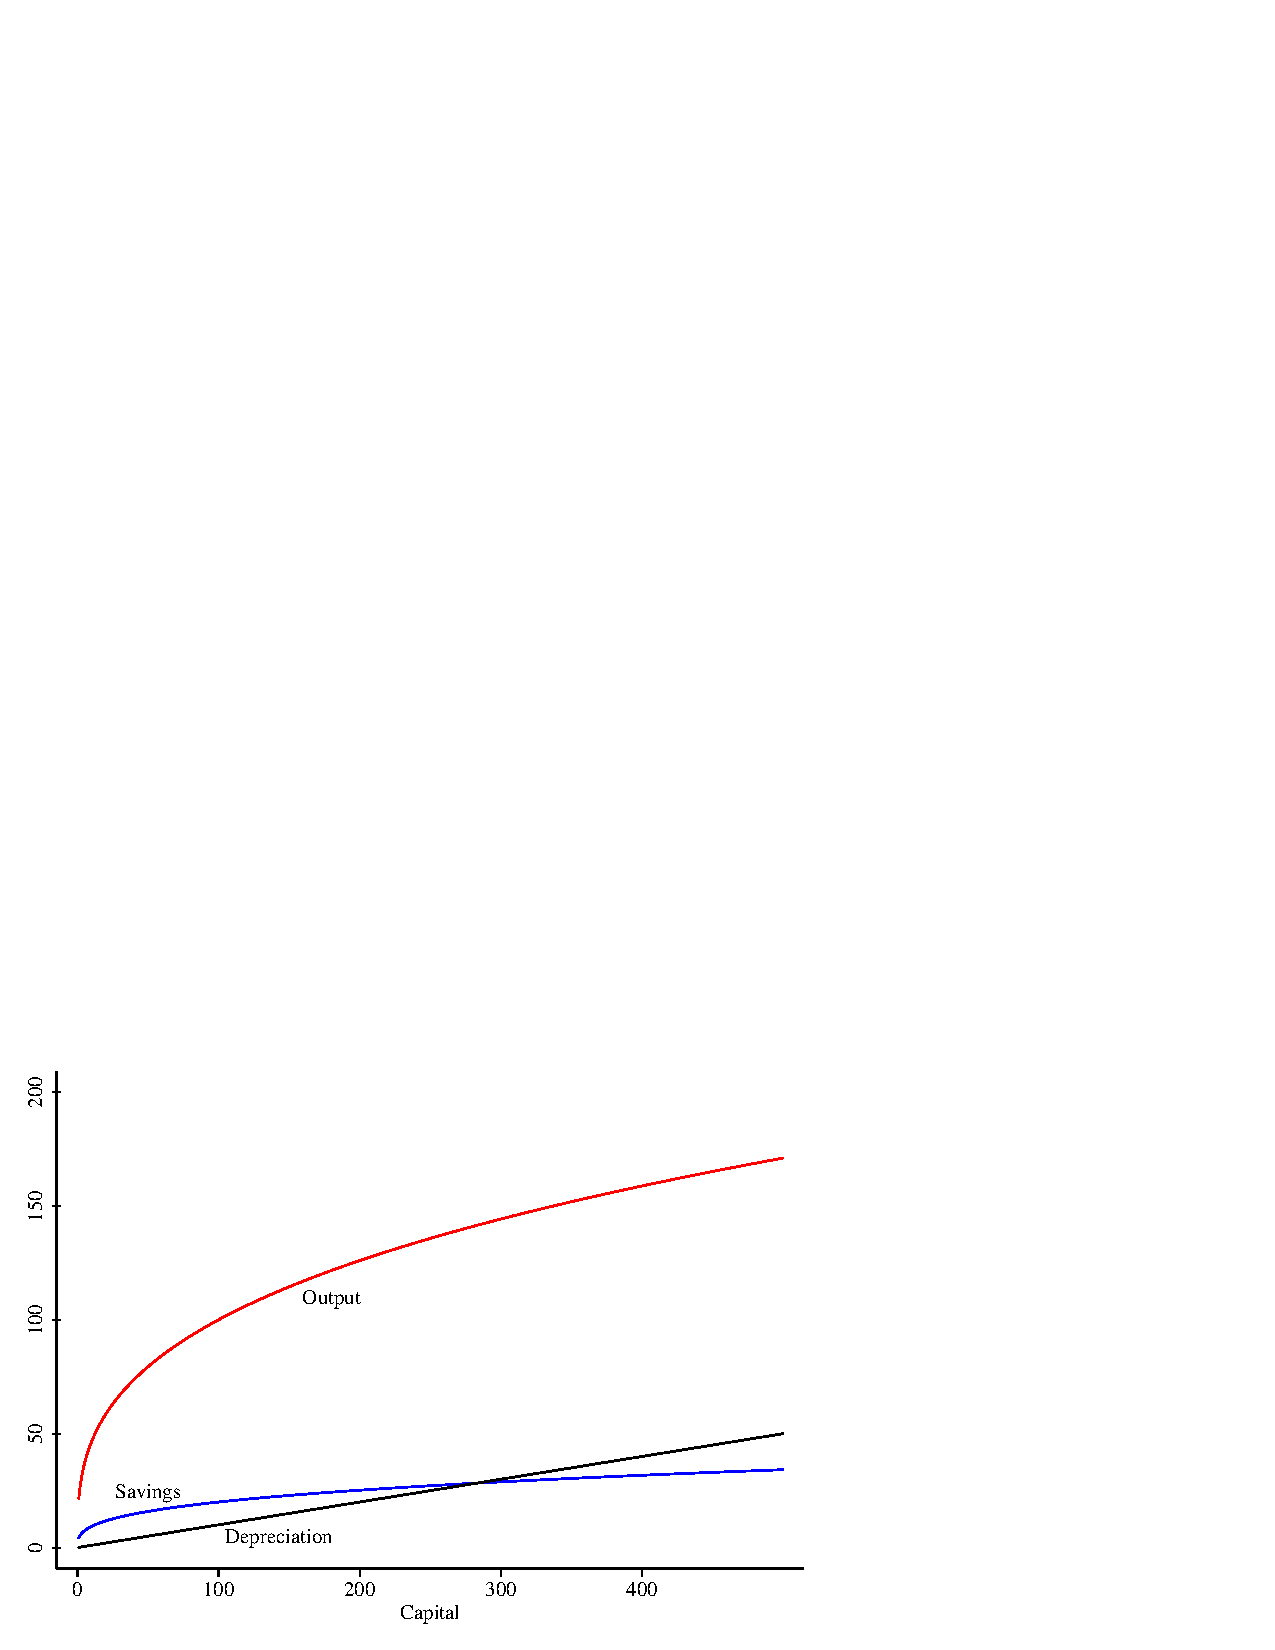
\includegraphics[width=0.8\textwidth]{\figpath Figures/solow1.pdf}\\
    \label{fig:solow1}
\end{figure}

What happens if we are above or below $K_{ss}$?
You can get a sense of the dynamics from Figure~\ref{fig:solow1}.
The top line is output,
which is related to the capital stock through the production function.
The next line is saving, a constant fraction of output
and the first expression on the right side of equation (\ref{eq:dK}):  $s A K^\alpha L^{1-\alpha} $.
The third line is depreciation, a constant fraction $\delta$
of the capital stock and the second object on the right side of equation (\ref{eq:dK}):  $\delta K $.
Diminishing returns to capital gives the saving line its curvature.
It leads to higher saving than depreciation at low
values of the capital stock, so the capital stock is increasing.
Similarly, saving is lower than depreciation at high values of the capital stock,
so the capital stock falls.
The crossing point is $K_{ss}$, where saving is just enough to
make up for depreciation, leaving the capital stock unchanged.


\section{Convergence\index{Solow model!convergence}}

The central feature of the model is what we call the convergence property:
If countries have the same parameters, they will eventually converge to the same
level of output per worker.
We haven't quite shown this yet, but the only thing missing
is the ``per worker'' qualification.


Consider, then, a version of the model in per-worker terms.
The first step is to divide both sides of (\ref{eq:k-lom}) by $L$.
If $k \equiv K/L$ is capital per worker (or the capital-labor ratio), the equation becomes
\begin{eqnarray*}
   k_{t+1} &=& (1-\delta) k_t + s A k_{t}^{\alpha}
\end{eqnarray*}
or
\begin{eqnarray}
   \Delta k_{t+1} &\equiv& k_{t+1} - k_t
            \;\;=\;\; s A k_{t}^{\alpha} - \delta k_t  .
   \label{eq:dk}
\end{eqnarray}
You'll note a resemblance to equation (\ref{eq:dK}).

Figure~\ref{fig:solow2} illustrates the model's dynamics.
It's based on the same parameter values as our earlier example:
$ A = 1$, $s = 0.2$, $\delta = 0.1$, and $\alpha = 1/3$.
\begin{figure}[ht]
\caption{The impact of the saving rate in the Solow model.}
    \label{fig:solow2}
    \centering
    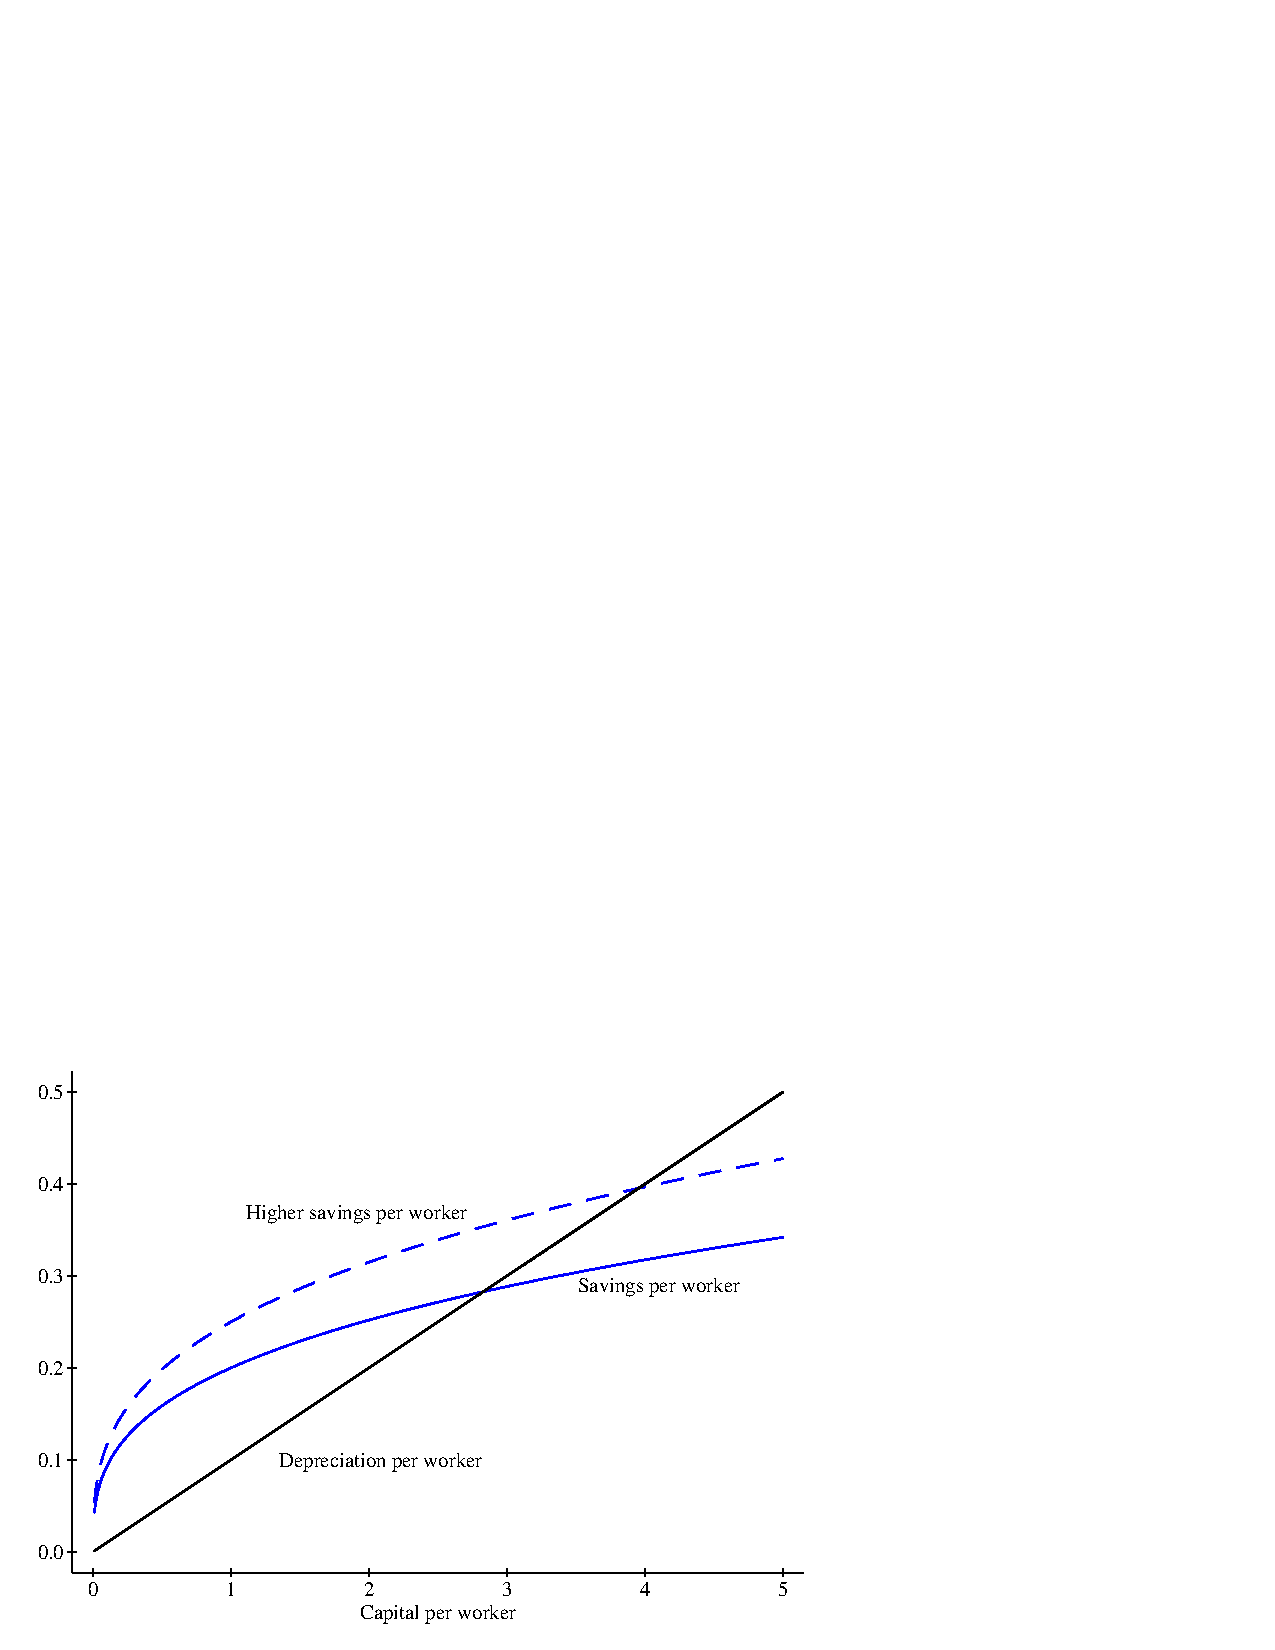
\includegraphics[width=0.8\textwidth]{\figpath Figures/solow2.pdf}\\
\end{figure}
The line marked ``saving per worker'' is the first expression on
the right side of equation (\ref{eq:dk}):  $ s A k^\alpha $. The
line marked ``depreciation per worker'' is the second expression
on the right side of equation (\ref{eq:dk}):  $\delta k$. For
small values of $k$, saving per worker is greater than
depreciation per worker, so $k$ increases. For large values of
$k$, saving per worker is less than depreciation per worker, so
$k$ decreases. The two lines cross at the steady state, where the
capital-labor ratio is constant. We can find the steady-state
value of $k$ from equation (\ref{eq:dk}) by setting $\Delta
k_{t+1} = 0$.  This leads to
\[
    k_{ss} \;=\; \left( \frac{sA}{\delta} \right)^{1/(1-\alpha)} ,
\]
a minor variant of our earlier expression for the steady-state capital stock.


We have shown that the capital-labor ratio eventually converges to its steady-state value.
What about output per worker?
The production function in per worker form is $ Y/L = A k^\alpha$,
so steady-state output per worker depends on steady-state capital per worker:
\begin{equation}
    (Y/L)_{ss}  \;\;=\;\; A k_{ss}^\alpha
                \;\;=\;\; A \left( \frac{sA}{\delta} \right)^{\alpha/(1-\alpha)}
                \;\;=\;\; A^{1/(1-\alpha)} \left( \frac{s}{\delta}
                \right)^{\alpha/(1-\alpha)} .
                \label{eq:ss-yl}
\end{equation}
Similarly, the steady-state capital-output ratio is
\[
    (K/Y)_{ss} \;\;=\;\; \left( \frac{s}{\delta} \right) .
\]
The algebra isn't pretty, but it tells us how the steady state
depends on the various parameters.
The last equation tells us, for example, that countries with higher saving rates
also have higher steady-state capital-output ratios --- that is more saving leads to more capital.
Equally important, the existence
of a steady state tells us that if two countries have the same
parameter values, they will converge to the same output per
worker. We refer to this as the convergence   property. In this
model, any long-term differences between countries must come from
differences in their parameters.


\section{Impact of saving \index{saving} and investment}

We can return to the question we began with: What is the impact of saving
and investment rates on growth and income?
The long-run impact of saving \index{saving}
on growth is zero;
the steady-state growth rate is zero, regardless of the saving rate.
But there is an effect of saving on steady-state output per worker.

Consider our example.
From equation (\ref{eq:ss-yl}), we see that steady-state
output per worker is 1.4142.
What if we increase the saving rate $s$ from 20 percent to 25 percent?
Then, steady-state output rises to 1.5811, an 11 percent increase.
This isn't irrelevant, but it's a relatively modest increase
for a substantial increase in saving.
It clearly does not explain much of the enormous differences
in GDP per capita that we see around the world.

We can see the same thing in Figure~\ref{fig:solow2}. The line marked
``saving per worker'' is based on a saving rate of $s = 0.20$, or
20 percent. If we raise the saving rate to  25 percent,
the saving line shifts up, as
shown by the dashed line marked ``higher saving per worker.'' Why?
Because $s A k^\alpha $ is higher at every value of $k$. With this
new line, the steady-state value of capital per worker (where the
saving line crosses the depreciation line) is higher, as shown.\index{Solow model|)}


\section{Growth}

If saving doesn't generate growth, what does?
We add growth in the labor force and
(critically) growth in total factor productivity
with two goals in mind.
The first goal is to account for the growth rate of output,
showing how it depends on the growth rates of our two inputs.
The second is to show that the economy approaches
what we call a balanced growth path in which
output and capital grow at the same rate.
As before, the capital-output ratio approaches a constant,
the features of which we can easily summarize.
We do this with a striking example in mind:
We know that China invests an astounding 40 percent of its GDP.
Is this too much?
A hint is that capital intensity
(measured by the capital-output ratio)
depends not only on the investment rate (which tells us how
much new capital is added), but also on the growth rate
(how fast the denominator is changing).
A fast-growing economy needs a high investment rate
simply to maintain a given capital-output ratio.


The new inputs into our analysis are growth in the   labor force \index{labor!labor force}
and productivity.
Let us say, to be concrete,
that labor and productivity grow
at constant rates:
\begin{eqnarray*}
    L_{t+1} &=&  (1+g_l) L_t \\
    A_{t+1} &=&  (1+g_a) A_t .
\end{eqnarray*}
How fast do output and capital grow?
Let's guess that output and capital grow at the same rate $g_y$,
to be determined.
(Why?  Because we're good guessers.)
From the production function, we then know that
\begin{eqnarray*}
    (1+g_y)       &=& Y_{t+1}/Y_t  \\
                &=&  (A_{t+1}/A_t) (K_{t+1}/K_t)^\alpha
                        (L_{t+1}/L_t)^{1-\alpha} \\
                &=& (1+g_a) (1+g_y)^{\alpha} (1+g_l)^{1-\alpha} .
\end{eqnarray*}
The growth rate, is therefore,
\begin{eqnarray*}
    (1+g_y)       &=& (1+g_a)^{1/(1-\alpha)} (1+g_l) .
\end{eqnarray*}
Just a formula, but it says that output growth is tied
to the growth rates of productivity and labor.
The saving rate does not affect this growth rate.
Similarly, the growth rate in output per worker is
\begin{eqnarray*}
    (1+g_y)/(1+g_l)     &=& (1+g_a)^{1/(1-\alpha)} ,
\end{eqnarray*}
which depends only on productivity growth.
If $\alpha$ is positive,
the growth rate of output per worker is
higher than the growth rate of productivity,
because the exponent $ 1/(1-\alpha)$ is greater than one.
In words, the direct impact of productivity on output
is magnified by the growth in the stock of capital;
see the production function (\ref{eq:pf_solow}).
This ties in with a remark we made earlier: That capital accumulation
tends to reinforce the impact of productivity growth.
Countries with high productivity also have a lot of capital.


What about capital --- do countries with higher saving rates have more
capital, relative to the size of their economies?
Consider, again, a steady state in which capital and output grow
at the same rate $g_y$.
Then $K_{t+1} = (1+g_y) K_t$ and equation (\ref{eq:k-lom}) becomes
\begin{eqnarray*}
    K_{t+1}  &=& (1-\delta) K_t + s Y_t  \\
    (1+g_y) (K_{t}/Y_{t}) &=& (1-\delta) (K_t/Y_t) + s .
\end{eqnarray*}
Solving for $K/Y$ gives us the steady-state capital-output ratio:
\begin{eqnarray*}
    (K/Y)_{ss} &=& \left( \frac{s}{\delta+g_y} \right) .
\end{eqnarray*}
%This line of argument doesn't actually require the Solow model.
%If we divide equation (\ref{eq:k-lom})
%by $Y_t$ and substitute $ Y_{t} =  Y_{t+1}/(1+g)$, we get
%\begin{eqnarray*}
%    (1+g) K_{t+1}/Y_{t+1}  &=& (1-\delta) K_t/Y_t + s .
%\end{eqnarray*}
%The steady state capital-output ratio
%(the ratio that makes $K_{t+1}/Y_{t+1}$ and $K_{t}/Y_{t}$ equal)
%is exactly what we just derived.

To return to our goal of understanding the sources of capital intensity,
note the impact of growth on the steady-state capital-output ratio.
For a given saving/investment rate $s$, countries with higher growth $g_y$
will have relatively less capital per unit of output.
Why?  Because when output is growing quickly,
you need to invest a lot to keep capital growing at the same rate.


\textbf{Example.}
Here are some numbers based loosely on the US:
$ g_l = 0.005 $ (0.5\%), $ g_a = 0.01 $ (1\%), $s=0.15$,
and $\delta = 0.06$.
What is the growth rate of output?
The steady-state capital-output ratio?
The growth rate satisfies
\[
    1+g_y \;\;=\;\; (1+g_a)^{1/(1-\alpha)} (1+g_l) \;\;=\;\; 1.015 \times 1.005
        \;\;=\;\; 1.0201.
\]
Here, we've used $\alpha = 1/3$, as usual.
Using the same parameters as our earlier examples, the steady-state
capital-output ratio is
\[
    1.872 \;\;=\;\; \frac{0.15}{0.06 + 0.020} .
\]
Now consider numbers based on China.
We keep $ g_l = 0.005 $ and $\delta = 0.06$,
but change the others to $ g_a = 0.05 $ and $s = 0.40 $.
The growth rate is now $g_y = 0.0813$ and the capital-output ratio
is 2.83. Note the moderate increase, despite the near tripling of the
saving/investment rate. Is China investing too much?
Perhaps not. Their capital-output ratio (by this calculation)
is not much different from that of the US, so the 40\% investment
rate isn't delivering excessive capital intensity by this measure.
They need to invest a lot simply to keep up with the growth
of their economy.


%\subsubsection*{Discussion}


%[??] Solow's work focussed attention on saving and investment.
%If high per capita income required high saving, then maybe we should save more.
%And if it required investment, poor countries should think about
%financing investment through foreign borrowing as well as domestic saving.
%Our sense is that neither of these conclusions are supported by the evidence.
%High saving rates do finance greater investment,
%but they come at the cost of lower consumption rates.
%And poor countries, as we'll see, are poor primarily because they
%have low productivity, not because they lack capital.


\section*{Executive summary}

%\setlength{\leftmargini}{.5\oldleftmargini}
\begin{enumerate}
\item Solow's model bases growth on saving and investment.

\item Saving affects steady-state GDP per worker,
but not its growth rate.
In this sense and others, saving is secondary to long-term
economic performance.

\item
%The steady state capital-output ratio depends
%on both the saving rate and the growth rate of the economy.
Fast-growing countries must invest more to maintain the same
capital-output ratio.
\end{enumerate}
%\setlength{\leftmargini}{\oldleftmargini}

\section*{Review questions}

%\setlength{\leftmargini}{.5\oldleftmargini}
\begin{enumerate}

\item The basics.  Suppose $A=L=K=1$, $\alpha = 1/3$, $\delta = 0.06$, and $s = 0.12$.
\begin{enumerate}
\item What is output $Y$?
\item What are saving $S$ and investment $I$?
\item What is next period's capital stock?
\end{enumerate}

\needspace{4\baselineskip}
Answer.
\begin{enumerate}
\item $Y = A K^{1/3} L^{2/3} = 1$.
\item $S=I = s Y = 0.12$.
\item Put $t$'s on everything so far.
Then $K_{t+1} = (1-\delta) K_t + I = 0.94 + 0.12 = 1.06$.
\end{enumerate}


\item Example, continued.  For the numerical example in the text:
\begin{enumerate}
\item Suppose that the economy starts with the steady-state capital stock.
What are the steady-state levels of output, investment, and consumption?
\item If 25 percent of the capital stock is destroyed in a war,
how long does it take the economy to eliminate half the fall in output?
\end{enumerate}

\needspace{4\baselineskip}
Answer.
\begin{enumerate}
\item The steady-state capital stock is (as we've seen) $K_{ss} = 282.8$.
Using this value, the production function tells us that output is 141.4.
Investment equals the depreciation of the capital stock, 28.3.
We can find consumption in two ways.
The first is through the expenditure identity:  $Y = C + I$.
We know $Y$ and $I$, so $C$ is 113.1.
The second is through the flow identity.
Saving is fraction $s$ of output, so consumption is fraction $1-s$,
$ 0.8 \times 141.4 = 113.1 $.
\item This requires a simulation.
Let the capital stock fall to 212.1, 75 percent of its steady-state value.
Then, output is 128.5, 90.9 percent of its steady-state value.
We recover half the fall if output rises to 135.0.
If we simulate the model, we see that it reaches 135.1 in 10 periods (years).
\end{enumerate}

\item Government.  We've ignored government so far.  Suppose, instead,
that the government purchases goods and services
equal to a constant fraction of GDP
(say, $ G = d Y$ for some fraction $d$)
 and collects taxes equal to the same fraction of output.
Individuals have after-tax income of $ (1-d) Y$ and save a
fraction $s$ of it.
With these changes, how would the analysis of the basic Solow model change?

Answer.  The critical ingredient here is the fraction of output allocated
to investment.
Investment here is $ I = S = s (1-d) Y $.
Effectively, $d$ reduces the saving rate from $s$ to $s(1-d)$
and takes resources away from investment.
If the government invests, we'd have to include that,
but we'd also have to decide how useful the investment was
(does it count the same as other investment?).

\begin{comment}
% ?? answer needs help
\item Population growth.
Consider the model with population growth, and suppose
that $\delta = 0.1$, $s = 0.2$, $A = 1$, and $g_l = 0.01$. How much does
steady-state output per worker fall if $g_l$ rises to 0.02? \\
Warning:  This is moderately difficult.
You can't apply a formula from the text,
you need to work out the steady state on your own.

Answer.  In this case and others like it,
what's constant in a steady state is $K/Y$,
meaning $K$ and $Y$ grow at the same rate.
Call this rate $g$; it implies, for example,
$ Y_{t+1} = (1+g) Y_t$, and the same for $K_t$.
The critical inputs are the dynamics of capital and the production function.
Let's take them one at a time.

(i) Capital.  Consider the dynamics of
capital in a steady state.
We divide equation (\ref{eq:k}) by $Y_t = Y_{t+1}/(1+g)$ to get
\begin{eqnarray*}
    (1+g) (K_{t+1}/Y_{t+1}) &=& (1-\delta) (K_t/Y_t) + s.
\end{eqnarray*}
In a steady state where $K/Y$ is constant, we have
$ (g+\delta) (K/Y) = s $.

(ii) Production function.  Take the ratio of equation
(\ref{eq:pf_solow}) at date $t+1$ to the same equation at date $t$:
\begin{eqnarray*}
    (Y_{t+1}/Y_t) &=& (A_{t+1}/A_t) (K_{t+1}/K_t)^\alpha (L_{t+1}/L_t)^{1-\alpha} .
\end{eqnarray*}
Our assumptions about growth rates gives us
$ (1+g) = (1+g)^\alpha (1+g_l)^{1-\alpha} $,
or $ (1+g) = (1+g_l)$.
Returning to (i), we see that
$ K/Y = s/(g_l+\delta) $.

(iii) Output per worker.
The last step is to make the shift from $K/Y$ to $Y/L$.
We divide the production function by $K$, giving us
\begin{eqnarray*}
    (K/L)^{1-\alpha} &=& A (K/Y)
        \;\;\;\Rightarrow\;\;\;
        K/L \;\;=\;\; \left( \frac{ A s}{g_l + \delta} \right)^{1/(1-\alpha)}.
\end{eqnarray*}

Now we can do the calculations.
With $g_l=0.01$, steady-state output per worker is 1.348.
When $g_l=0.02$, it falls to 1.291, a drop of about 4 percent.
\end{comment}



\end{enumerate}
%\setlength{\leftmargini}{\oldleftmargini}

\section*{If you're looking for more}

This material is covered in many macroeconomics textbooks.
Our favorites are
\begin{itemize}
\item Tyler Cowen and Alex Tabarrok,
{\it Modern Principles: Macroeconomics\/}, ch 7.
\item N. Gregory Mankiw, {\it Macroeconomics (6th edition)\/}, chs 7-8.
\end{itemize}
Any editions will do, but the chapter numbers may vary.


Goldman Sachs has used the Solow model
(and some heroic assumptions about fundamentals) to forecast the importance of
the BRICs (Brazil, Russia, India, and China)
to the world economy in 50 years.
See
``\href{http://www.goldmansachs.com/korea/ideas/brics/99-dreaming.pdf}
{Dreaming with BRICs}.''
It's a good example of how assumptions about productivity, population growth, and education can be used to generate plausible scenarios for the sizes of economies in the distant future.
(The equations on their page 18 should look familiar.)
This doesn't make forecasting any less hazardous, but it tells you
what the critical inputs are.
The key one here, of course, is productivity growth.

\section*{Symbols used in this chapter}

\begin{table}[H]
\centering
\caption{Symbol table.}
\begin{tabular*}{0.95\textwidth}{l@{\extracolsep{\fill}}l}
\toprule
Symbol & Definition\\
\midrule
$Y$                            &Output (real GDP)\\
$A$                            &Total factor productivity (TFP)\\
$K$                            &Stock of physical capital  (plant and equipment)\\
$L$                            &Quantity of labor (number of people employed)\\
$F(K,L)$                    &Function of inputs K and L in production function\\
$\alpha$                     &Exponent of $K$ in Cobb-Douglas   production function \\
                            &(= capital share of income)\\
$S$                            &Saving\\
$I$                            &Investment\\
$C$                            &Consumption\\
$s$                         &    Saving rate as a percent of income $Y$\\
$\delta$                     &Rate of depreciation of physical capital \\
$\Delta K$                    &Change of $K$ ($=K_{t+1}-K_{t}$)\\
$K_{ss}$                    &Steady-state capital stock\\
$(K/Y)_{ss}$                &Steady-state capital-output ratio\\
$k$                         &Capital per worker, or capital-labor ratio ($=K/L$)\\
$g_y$                     &Discretely-compounded growth rate of $Y$\\
$g_l$                     &Discretely-compounded growth rate of $L$\\
$g_a$                     &Discretely-compounded growth rate of $A$\\
$d$                         &Government purchases as a share of output $(G/Y)$\\
\bottomrule
\end{tabular*}
\end{table}


\chapter{Sources of Economic Growth}\label{chp:grth}
\hypertarget{growth}{}

%No extra line here.
\textbf{Tools:} Cobb-Douglas production function; level and growth accounting; continuously-compounded growth rates.

\textbf{Big Ideas:}
%\vspace{-0.1in}
\begin{itemize}
    \item Level and growth accounting allow us to \emph{quantify} the sources of growth: the contributions of capital, labor, and total factor productivity (TFP) to growth in real GDP.
    \item TFP accounts for most of the cross-country differences in output per worker and in differences in the growth rate of output per worker.
\end{itemize}

\rule{\textwidth}{1pt}

If saving rates aren't responsible for
the enormous differences we see in living standards, what is?
The answer is productivity, but our purpose here is to develop
a tool that will give us the answer, whatever it might be.
Our ingredients are data (always a good thing)
and a little bit of theory (the production function).
The combination allows us to attribute differences in output and its
growth rate to differences in inputs (capital and labor)
and total factor productivity (everything else).
The answer, as noted, is mostly productivity:
Rich countries are rich because they're productive,
and countries that are growing quickly typically
have rapid productivity growth, as well.
Robert Solow gets credit for this line of thought, too.


\section{Cross-country differences in output per worker}

%In class we've looked at per capita GDP as measure
%of aggregate performance:  output/income per person.
%Here we'll look at GDP per worker.  The two are connected by
%\begin{eqnarray}
%    Y/\POP &=& (Y/L) (L/\POP) .
%\end{eqnarray}
%Any differences in GDP per capita reflect either GDP per worker
%or the ratio of workers to population.
%We'll focus on the former now, but return to the latter
%when we get to labor markets.

The production function gives us some insight into cross-country differences
in GDP per worker.
You'll recall that the production function \index{production function}
 connects an economy's output
(real GDP)
to the quantity of inputs used in production (capital and labor)
and the efficiency with which those inputs are used (productivity).
In equation form:\index{gross domestic product (GDP)!real GDP}\index{growth accounting|(}
\begin{equation}
    Y \;=\; A F(K,L) \;=\; A K^\alpha L^{1-\alpha},
    \label{eq:pf_source}
\end{equation}
where (as before)
$Y$ is real GDP or output,
$A$ is total factor productivity (TFP),\index{productivity!total factor productivity (TFP)|(textbf}
$K$ is the capital stock,
and $L$ is the quantity of labor (typically employment).
More commonly, we divide both sides by $L$ and
express output per worker as
\begin{equation}
    Y/L \;=\;  A (K/L)^\alpha ,
    \label{eq:YL}
\end{equation}
so that output per worker depends on total factor productivity
($A$) and capital per worker ($K/L$).
%Our ability to convert this into a relation in ratios follows from the
%constant-returns-to-scale property of the production function.
For most countries, we have reasonably good data for GDP,
employment, and the capital stock,
and productivity can be found as a residual:
\begin{equation}
    A \;=\; {Y}/(K^\alpha L^{1-\alpha}) .
\end{equation}
We'll continue to use $\alpha = 1/3$, so there is nothing about
equations (\ref{eq:pf_source}) and (\ref{eq:YL}) that we don't know.
In this sense, the production function is no longer an abstract idea,
but a practical tool of analysis.


\begin{table}[h]
\centering
\caption{Data for Mexico and the US.}
\begin{tabular*}{0.8\textwidth}{l@{\extracolsep{\fill}}cccc}
\toprule
%\cline{2-7}%
                &   Employment   & Education & Capital  & GDP \\%
\midrule
Mexico          &     46.94    &    7.61    &  4,278   &  1,293 \\%
%\hline%
US              &    155.45    &    12.27   & 42,238   &  12,619 \\%
\bottomrule
\addlinespace
\end{tabular*}
\begin{minipage}{0.8\textwidth}
\footnotesize{{\small Aggregate data for 2009 (education for 2007).
Employment is expressed in millions, education in years,
and capital and GDP in billions of 2005 US dollars.
}}
\end{minipage}
\label{tab:mexus}
\end{table}

The production function allows us to make explicit
comparisons across countries.  If we apply equation (\ref{eq:YL})
to two countries  and take the ratio, we get
\begin{equation}
    \frac{(Y/L)_1}{(Y/L)_2} \;=\;
             \left[ \frac{A_1}{A_2} \right]
             \left[ \frac{(K/L)_1}{(K/L)_2} \right]^\alpha ,
        \label{eq:levelcomp}
\end{equation}
where the subscripts 1 and 2 refer to the two countries.
The ratio of output per worker is, thus, attributed to
some combination of the ratios of
TFP and capital per worker.
Exercises based on (\ref{eq:levelcomp}) are referred to as
{\it level comparisons\/}.\index{level accounting}
If we have data, we can say which of these factors is most important.

If we did this in logarithms, the components would add rather than multiply.
As a result, the contribution of each component can be expressed as a 
fraction the total.
We were tempted to do this, but worried it would unduly try your patience. 


\textbf{Example (Mexico and US).} You occasionally hear
people in the US say that Mexican workers are paid so much less
that they pose a threat to American jobs. (In Mexico, you hear the
same thing about Chinese workers.) We can't address that issue (yet) but we can say something about the source of differences
in output per worker, which is closely related to differences in
wages. The data in Table \ref{tab:mexus} imply that output per
worker is 2.95 times higher in the US, but why?
We'll use the data in Table~\ref{tab:mexus} to come up with an answer.

Let's start with TFP.
For Mexico, the data in the table imply that
\[
    A_M \;=\; 1293 / [ 4278^{1/3} 46.94^{2/3} ] \;=\; 6.12.
\]
A similar calculation for the US gives us $A_{US} = 12.53$.
Thus, TFP is 2.05 ($= 12.53/6.12$) times higher in the US.
Similarly, the capital-labor ratio is 2.98 times higher in the US.
The impact on output per worker is summarized by
\begin{eqnarray*}
     \frac{(Y/L)_{US}}{(Y/L)_{M}}  &=&  \frac{A_{US}}{A_M}
                        \left[ \frac{(K/L)_{US}}{(K/L)_{M}} \right]^{1/3} \\
                         &=&   (2.05) (2.98)^{1/3} \\ %\phantom{\sum^i} \\
                         &=&   (2.05) (1.44) \;=\; 2.95 . %\phantom{\sum^\infty}
\end{eqnarray*}
It seems, therefore, that both TFP and capital per
worker play a role in accounting
 for the
2.95-to-1 ratio of US to Mexican output per worker.
So the reason why output per worker is higher in the US is a
combination of higher productivity and
higher capital per worker.\index{level accounting}

This is your chance for speculation:
Why do you think the capital-labor ratio is lower in Mexico?
Why do you think productivity is lower?

%[Note: differences between the US and Mexico are smaller with this data,
%which has been PPP-adjusted, than if we had simply multiplied
%Mexican GDP by the exchange rate to express it in dollars. The
%reason:  many goods and services are cheaper in Mexico than the
%US, so when we apply the same prices to both countries the
%differences are smaller.
%See the discussion of PPP adjustment in
%the notes on national income and product accounts.]

%Our next task is to apply similar methods to
%account for differences in growth rates. Before proceeding, we
%need to be clear about what we mean by growth rates. For many
%purposes in this course, we will define the growth rate of a
%variable $x$ between dates $t$ and $t+1$ as
%\begin{equation}
%    \gamma \;=\; \ln x_{t+1} - \ln x_{t} \;=\; \Delta \ln x_{t+1} .
%\end{equation}
%The expression ``$\ln$'' here means the natural log,
%the function LN in a spreadsheet.
%We refer to $\gamma$ as the {\it continuously-compounded growth rate\/}
%for reasons we will ignore.
%(See the ``Math Review'' if you're interested.)
%Typically the dates are years, so $\gamma$ is an annual growth rate.
%If we want to express it as a percentage, we multiply by 100.
%The average growth rate between $t$ and $t+n$
%has a similar definition:
%\begin{equation}
%    \gamma \;=\; \left( \ln x_{t+n} - \ln x_{t} \right) / n  .
%\end{equation}
%The terminology here is that $\gamma$ is the average continuously compounded
%growth rate.
%
%You might want to know
%why aren't using the traditional definition of a growth rate,
%say $g$ in
%\begin{equation}
%    1 + g \;=\; x_{t+1}/x_t  \;\;\; \Leftrightarrow
%                \;\;\; g \;=\; (x_{t+1} - x_t)/x_t .
%\end{equation}
%Why use $\gamma$ rather than $g$?
%The answer is that what follows works out more neatly with $\gamma$.
%Otherwise we get the kinds of annoying compounding terms you might recall
%from bond \index{bond} pricing.
%
%You can stop here if you like; in fact,
%we order you to go immediately to the next section
%unless you are reasonably comfortable with mathematics.
%If you are, then here's a more elaborate explanation:
%\begin{itemize}
%\item There's little difference if the growth rates are small.
%This isn't an argument in favor of our definition, but it's good to know.
%Suppose $x_t = 100$ and $x_{t+1} = 110$.  Then $g = 0.100 $ and
%$\gamma = \ln 110 - \ln 100 = 0.0953$,
%so the growth rates are 10\% and 9.53\%.
%If the growth rate were smaller, the difference would be smaller, too.
%If you're not mathematically inclined, go immediately to the next point.
%If you are, we would tell you that $g$ is a first-order Taylor series approximation to $\gamma$.
%Note that $\gamma$ is a function of $g$:
%\[
%    \gamma \;=\; \ln x_{t+1} - \ln x_t \;=\; \ln (x_{t+1}/x_t) \;=\; \ln (1+g) .
%\]
%This follows from a property of logarithms:  $\ln x - \ln y = \ln(x/y)$.
%A first-order approximation of the function around the point $g=0$ is
%\[
%    \gamma \;\approx\; \ln (1) + (1) (g-0)  \;=\;  g,
%\]
%where ``$\approx$'' means ``approximately equal to.''
%Higher-order terms are $g^2/2$, $g^3/6$, and so on,
%which are very small if $g$ is small.
%
%\item Growth rates are additive.
%Suppose you're interested in the growth rate of a product $xy$.
%For example, $x$ might be the price deflator and $y$ real output, so that $xy$ is nominal output.
%With the traditional measure, the growth rate of $xy$ is
%\[
%    1 + g_{xy} \;=\; \frac{x_{t+1} y_{t+1}}{x_t y_t } \;=\; (1+g_x) (1+g_y).
%\]
%If $g_x = g_y = 0.10$, then $g_{xy} = 0.21$.
%But note what happens with our definition:
%\[
%    \gamma_{xy} \;=\; \ln \left( \frac{x_{t+1} y_{t+1}}{x_t y_t } \right)
%                \;=\; \ln \left( \frac{x_{t+1}}{x_t} \right) + \ln \left( \frac{y_{t+1}}{y_t} \right)
%                \;=\; \gamma_x + \gamma_y .
%\]
%They add up! Thus the growth rate of a product is the sum of the
%growth rates. That's not quite true for traditional growth rates,
%because of the ``compound interest'' effect:  $ (1+g_x) (1+g_y) =
%1 + g_x + g_y + g_x g_y$. The last term is small if the growth
%rates are, but it's not zero. This additive feature of continuously compounded growth
%rates is the primary reason we use them. For similar reasons, the
%continuously compounded growth rate of $x/y$ equals the growth rate of $x$ minus the
%growth rate of $y$.
%
%
%\item Averages are easy to compute.  Suppose we want to know the average growth rate of
%$x$ over $n$ periods:
%\[
%    \gamma \;=\; \frac{ (\ln x_{t+1}-\ln x_t) + (\ln x_{t+2}-\ln x_{t+1})
%                    + \cdots + (\ln x_{t+n} - \ln x_{t+n-1}) }
%                {n} .
%\]
%If you look at this for a minute, you might notice that most of the terms cancel.
%The term $\ln x_{t+1}$, for example, shows up twice, once with a positive sign, once with a negative sign.
%If we eliminate the redundant terms, we find that the average growth rate is
%\[
%    \gamma \;=\; \frac{ \ln x_{t+n}-\ln x_t }  {n}  \;=\; \frac{ \ln (x_{t+n}/x_t) }  {n} .
%\]
%We can compute it, then, from the initial and final values of $x$.
%
%\end{itemize}
%Finally, to go from growth rates back to levels,
%we need to use a method that corresponds to the growth rate we are using.
%For a traditional growth rate, we update levels by
%$ x_{t+1} = (1+g) x_t$.
%For continuously-compounded growth rates, we use
%$ x_{t+1} = \exp(\gamma) x_t $.


\section{Cross-country differences in growth rates}

Our next task is to apply similar methods to account for cross-country differences in \emph{growth rates} rather than levels.

\textbf{Warning, growth rates ahead:} Before you continue, you might want to go back and review
\hyperref[sec:growth_math_cc]{continuously-compounded growth rates}
in the Mathematics Review, Chapter \ref{chp:math}.

As before, the starting point is the production function.
If we take the natural logarithm of both sides of the production function (\ref{eq:pf_source}),
we find that
\[
    \ln Y_t \;=\;  \ln A_t + \alpha \ln K_t
            + (1-\alpha) \ln L_t
\]
for any date $t$.
This follows from two properties of logarithms:  $ \ln (xy) = \ln x + \ln y$
and $\ln x^a = a \ln x$.
If we take the difference between two adjacent periods $t$ and $t-1$ we get
\[
    \ln Y_t -  \ln Y_{t-1} \;=\;  (\ln A_t - \ln A_{t-1}) + \alpha (\ln K_t-\ln K_{t-1})
            + (1-\alpha) (\ln L_t - \ln L_{t-1}).
\]
Notice that each of the components should be recognizable as continuously-compounded   growth rates discussed in the \hyperref[sec:growth_math_cc]{growth-rate discussion}.

If we consider differences over $n$ periods, we can divide each term by the number of periods to get
\begin{eqnarray*}
    \left( \frac{ \ln Y_{t} - \ln Y_{t-n} }{n} \right) &=&
                    \left( \frac{\ln A_{t} - \ln A_{t-n}} {n} \right)
                    + \alpha \left( \frac{ \ln K_{t} - \ln K_{t-n}} {n} \right) \\
        && + \; (1-\alpha) \left( \frac{\ln L_{t} - \ln L_{t-n}} {n} \right).
\end{eqnarray*}
Notice that we have expressed the average, continuously-compounded   growth rate of GDP into the average, continuously-compounded growth rate of each component of the production function (i.e., TFP, capital, and labor). Using our notation convention that continuously-compounded   growth rates are represented by $\gamma$,
we can express the formula above more succinctly as
\begin{equation}
    \gamma_Y \;=\; \gamma_A + \alpha \gamma_K + (1-\alpha) \gamma_L.
    \label{eq:gammaY}
\end{equation}
In words, this equation says that the growth rate of output can be attributed to growth in TFP, capital, and labor. Moreover, the terms add up because of our use of logarithms and continuously compounded\index{growth rate!{continuously compounded}} growth rates. Additivity is nice, as it allows us to make statements about the contributions of each component to the growth of GDP.

As with levels, we can do the same for the growth rate of output per worker:
\begin{eqnarray}
    \gamma_{Y/L} &=& \gamma_Y - \gamma_L \nonumber \\
            &=&  \gamma_A + \alpha (\gamma_K - \gamma_L) \nonumber \\
        &=& \gamma_A + \alpha \gamma_{K/L} .
    \label{eq:gammaYL}
\end{eqnarray}
Exercises based on (\ref{eq:gammaY}) and (\ref{eq:gammaYL}) are referred to as
{\it growth accounting\/},\index{growth accounting} which allows us to make statements about the contributions of each component in accounting
 for the growth of GDP (\ref{eq:gammaY}) or GDP per worker (\ref{eq:gammaYL}).

Both versions of growth accounting
 give us some insight into the sources of economic
growth, as the example below shows.


\textbf{Example (Chile between 1965 and 2009).}
GDP increased by almost a factor of five between 1965 and 2009.
Can we say why? The relevant data are reported in Table \ref{tab:chile}.
\begin{table}[h]
\centering
\caption{Chilean aggregate data for 1965 and 2009.}
\begin{tabular}{lcccc}
\toprule
%\cline{2-7}%
                &   Employment   & Education & Capital  & GDP \\%
\midrule
1965            &     2.71    &    4.77   & 65.63  &  33.62 \\%
%\hline%
2009            &     7.52    &    7.97   & 819.81 & 199.2 \\%
\bottomrule
\end{tabular}
\label{tab:chile}
\end{table}

The first step is to compute growth rates.
Over this period, the average annual growth rate of real GDP was\index{gross domestic product (GDP)!real GDP}
\[
    \gamma_{Y} \;=\; \frac{\ln Y_{2009} -\ln Y_{1965}}{44}
            \;=\; (5.29-3.52)/44 \;=\; 0.0404,
\]
or 4.04 percent.
Using the same method,
we find that the growth rates of the other variables we need are
 $\gamma_{K}=5.74$ percent and $\gamma_{L}=2.32$ percent.
The growth rate of total factor productivity is the residual
in equation (\ref{eq:gammaY}):
\[
    \gamma_A \;=\; \gamma_Y - \left[ \alpha \gamma_K +
            (1-\alpha) \gamma_L \right]
                \;=\; 0.58\% .
\]
(You could also compute $A$ for each period
and calculate the growth rate directly.)
So why did output grow?
Our numbers indicate that of the 4.04 percent growth in output,
0.58 percent was due to TFP; 1.91 percent [$=5.74\times\frac{1}{3}$] was due to increases in capital;
and 1.55 percent [$=2.32 \times (2/3)$] was due to increases in employment.

What about output per worker?
That seems to be the more interesting comparison,
because it's closer to an average living standard.
The growth rate of output per worker is
$ \gamma_{Y/L} = 1.72$ percent.
Its components are
\begin{eqnarray*}
    \gamma_{Y/L} &=& \gamma_A + \alpha \gamma_{K/L} \\
      1.72   &= & 0.58 + (1/3) 3.42.
\end{eqnarray*}
In this case, most of the growth in output per worker came from
capital per worker, rather than TFP.\index{productivity!total factor productivity (TFP)|)}\index{growth accounting|)}


\section{Extensions}

We will sometimes use modifications of these tools.
Two of the more common ones are based on
(i) more-refined measures of labor
and/or (ii) GDP per capita rather than GDP per worker.
The logic is the same as before, but we gain an extra term or two.
%We recommend you skip this the first time through.


\textbf{Labor measures.} Consider a measure of labor that includes
adjustments for hours worked $h$ and human capital \index{capital!human capital} $H$.
If the labor input is $hHL$ (with $L$ the number of people employed),
the production function becomes
\begin{equation}
    Y \;=\; A F(K,hHL) \;=\; A K^\alpha (hHL)^{1-\alpha} .
    \label{eq:pf-aug}
\end{equation}
How does this change our analysis of levels and growth rates?
In a  level comparison, this leads to
\[
    \frac{Y_1}{Y_2} \;=\;
             \left[ \frac{A_1}{A_2} \right]
             \left[ \frac{K_1}{K_2} \right]^\alpha
             \left[ \frac{L_1}{L_2} \right]^{1-\alpha}
             \left[ \frac{h_1}{h_2} \right]^{1-\alpha}
             \left[ \frac{H_1}{H_2} \right]^{1-\alpha} .
\]
The subscripts 1 and 2 again represent countries.
You can derive further modifications for output per worker ($Y/L$)
and output per hour worked ($Y/hL$).
In a growth-rate analysis,
the augmented production function (\ref{eq:pf-aug})
leads to
\begin{eqnarray*}
    \gamma_Y &=& \gamma_A + \alpha \gamma_K + (1-\alpha)
        (\gamma_h + \gamma_H + \gamma_L)
\end{eqnarray*}
for output and
\begin{eqnarray*}
    \gamma_{Y/L} &=&  \gamma_A
                + \alpha \gamma_{K/L}
                    + (1-\alpha) (\gamma_h + \gamma_H ) \\
    \gamma_{Y/hL} &=&  \gamma_A
                + \alpha \gamma_{K/hL}
                    + (1-\alpha) \gamma_H
\end{eqnarray*}
for output per worker and output per hour, respectively.
If this sounds complicated, remember that the choice of tool
depends on the question we're trying to answer.

We have some choices when it comes to measuring human capital \index{capital!human capital} capital.
One simple choice is to equate human capital \index{capital!human capital} capital with years of school:
$H = S$ if we want to give it mathematical form.
A more sophisticated choice is to give education a rate of return,
so that
\begin{equation}
    H \;=\; \exp( \sigma S ) ,
    \label{eq:mincer}
\end{equation}
where $\sigma$ is kind of a rate of return on school,
as each year raises human capital \index{capital!human capital} capital proportionately.
Estimates of $\sigma$ are in the range of $0.07$,
so that each year of school raises human capital \index{capital!human capital} capital by
about $7$ percent.


\textbf{Per capita GDP. \index{gross domestic product (GDP)!per capita GDP}} The analysis above concerned GDP per worker (rather than per capita).
How can we adapt our analysis to account for GDP per capita?
Here's a trick:
start with equation (\ref{eq:YL}) and multiply both sides by
the ratio of employment to population:
\[
    Y/\POP \;=\; (L/\POP) (Y/L) \;=\; (L/\POP) A (K/L)^\alpha .
\]
In a level comparison, this gives us an extra term:  the ratio
of $L/\POP$ across countries.
In growth rates, we'd add an extra term for the growth rate of
the employment ratio:
\begin{eqnarray*}
    \gamma_{Y/POP} &=&  \gamma_{L/POP}  + \gamma_A
                + \alpha \gamma_{K/L}  .
\end{eqnarray*}
And if you want to get fancy, you can add hours and human-capital\index{capital!human capital} terms,
as we did above.


\textbf{Example (Mexico and US, revisited).}
How does our analysis of the US and Mexico change if
we incorporate differences in human\index{capital!human capital} capital?
We set human capital\index{capital!human capital} $H$ equal to years of school
and redo our earlier analysis.
TFP is now
\[
    A_M \;=\; 1293 / [ 4278^{1/3} (7.61 \times 46.94)^{2/3} ] \;=\; 1.58
\]
for Mexico and $A_{US} = 2.36$ for the US.
Note that the ratio has fallen from 2.05 to 1.49.
Why?  Because part of the previous difference
now shows up in human\index{capital!human capital} capital.
[Reminder:  $A$ is a residual, so
any change in the analysis changes our measure of it.]
We now attribute some of the difference in output per worker
to a difference in education:
\begin{eqnarray*}
     \frac{(Y/L)_{US}}{(Y/L)_{M}}  &=&  \frac{A_{US}}{A_M}
                        \left[ \frac{(K/L)_{US}}{(K/L)_{M}} \right]^{1/3}
                        \left[ \frac{H_{US}}{H_M} \right]^{2/3}_{\phantom{X_X}}   \\
                         &=&   (1.49) (2.98)^{1/3} (1.61)^{2/3}  \\%\phantom{\sum^i} \\
                         &=&   (1.49) (1.44) (1.38) \;=\; 2.95 . %\phantom{\sum^\infty}
\end{eqnarray*}
It appears that more than half of our earlier difference in TFP\index{productivity!total factor productivity (TFP)}
stems from differences in education.
We amend our previous analysis to add:
A substantial part of the difference between output per worker
in the US and Mexico stems from differences in education.

An alternative is to measure human\index{capital!human capital} capital using our
rate-of-return formula, equation (\ref{eq:mincer}).
If we do this, the ratio of human\index{capital!human capital} capital is 1.39,
which is less than we had before.
This choice makes an even bigger difference with countries
like India, which have low average education.
If years of school go from two to three, is that a 50-percent increase
in human\index{capital!human capital} capital or a seven-percent increase?
You be the judge.
Of course, it may depend on what they learn in school, too.


\section*{Executive summary}

%\setlength{\leftmargini}{.5\oldleftmargini}
\begin{enumerate}
\item Recall that a production function links output to inputs and productivity.

\item Therefore, differences in output and growth rates across countries
stem from differences in the levels and growth rates
of inputs and productivity (TFP).\index{productivity!total factor productivity (TFP)}

\item Level accounting\index{level accounting} and growth accounting\index{growth accounting}
 allows us to quantify the differences in output and growth arising from differences in inputs and total factor productivity.
\end{enumerate}
%\setlength{\leftmargini}{\oldleftmargini}

\section*{Review questions}

%\setlength{\leftmargini}{.5\oldleftmargini}
\begin{enumerate}
\item Growth rates.  Take the following data:
%
\begin{center}
\begin{tabular}{lcc}
\toprule
                & Output $Y$  & Employment $L$ \\
\midrule
1950 \hspace*{0.25in} &  10 & 2 \\
2000  &  50 & 3 \\
\bottomrule
\end{tabular}
\end{center}
%
\begin{enumerate}
\item What are the average annual continuously-compounded   growth rates of $Y$ and $L$?
\item What is the analogous growth rate of $Y/L$?
\end{enumerate}

Answer.
\begin{enumerate}
\item The growth rate of output is
\begin{eqnarray*}
    \gamma_Y &=& [\ln (50) - \ln (10)]/(2000-1950) \;\;=\;\; 0.0322 ,
\end{eqnarray*}
or 3.22\% per year.
A similar calculation gives us $\gamma_L = 0.0081$ = 0.81\% per year.
\item We can do this two ways.  The easiest is
\begin{eqnarray*}
    \gamma_{Y/L} &=& \gamma_{Y} - \gamma_{L} \;\;=\;\; 0.0241.
\end{eqnarray*}
You can also compute it by dividing $Y$ by $L$
and applying the same method we used in (a).
\end{enumerate}

\item France and the UK.  In 2007, the data were:
%
\begin{center}
\begin{tabular}{lcccc}
\toprule
%\cline{2-7}%
                &   Employment   & Education & Capital  & GDP \\%
\midrule
France  &  29.51 &  8.48 &  6,478 &  1,986 \\
UK      &  31.79 &  9.88 &  5,243 &  2,070 \\
\bottomrule
\end{tabular}
\end{center}
%
Which country had higher output per worker?  Why?
You should assume that human\index{capital!human capital} capital is equal to years of school.

Answer.  Ratios were as follows:
\begin{eqnarray*}
    \left( \frac{(Y/L)_{F}}{(Y/L)_{UK}} \right) &=& \left( \frac{A_{F}}{A_{UK}} \right)
                        \left( \frac{(K/L)_{F}}{(K/L)_{UK}} \right)^{1/3}
                        \left( \frac{H_{F}}{H_{UK}} \right)^{2/3}  \\
            1.03              &=&   (1.04) (1.33)^{1/3} (0.86)^{2/3}  . \phantom{\sum^\infty}
\end{eqnarray*}
That is, France had slightly higher TFP and more capital per worker,
but a lower level of education than the UK.
%Note, too, that France has a better soccer team.

\item US and Japan.
Explain why output grew faster in Japan between 1970 and 1985.
Data:
%
\begin{center}
\small
\begin{tabular*}{0.9\textwidth}{lcrrccrrc}
\toprule
&&  \multicolumn{3}{c}{United States} && \multicolumn{3}{c}{Japan}        \\
                        \cmidrule{3-5}  \cmidrule{7-9}
&&              1970  & 1985 & Growth && 1970 & 1985 & Growth \\
\midrule
GDP && 2083 &  3103  &  2.66    &  &   620  & 1253  &  4.69   \\
Capital      && 8535 & 13039  &  2.83    &  &  1287  & 3967  &  7.50   \\
Labor  && 78.6 & 104.2  &  1.88    &  &  35.4  & 45.1  &  1.61   \\
\bottomrule
\end{tabular*}
\end{center}
%
Employment is measured in millions of workers,
GDP and capital in
billions of 1980 US dollars.
Growth rates are continuously-compounded average annual percentages.

Answer.
In levels (as opposed to growth rates), we see that
the US had much greater output per worker in 1970:
26.5 (thousand 1980 dollars per worker) vs 17.5.
Where did this differential come from?  One difference is that American
workers in 1970 had three times more capital to work with:
$K/L$ was 108.6 in the US, 36.4 in Japan.  If we use our production
function, we find that total factor productivity $A$
was also slightly higher in the US in 1970:  5.55 v. 5.29.
Thus, the major difference between the countries in
1970 appears to have been in the amount of capital:  American workers had more
capital and, therefore, produced more output, on average.

By 1985, much of the difference had disappeared.
%It's obvious from the
%numbers that the biggest difference between Japan and the US over the 1970-85
%period is in the rate of growth of the capital stock.
For the US, the output growth rate of 2.66 percent per year can be divided
into 0.94 percent due to capital and 1.26 percent due to employment growth.
That leaves 0.47 percent for growth in total factor productivity.
For Japan, the numbers are 2.48 percent for capital, 1.08 percent for
labor, and 1.13 percent for productivity.
Evidently, the largest difference between the two
countries was in the rate of capital formation:  Japan's capital stock
grew much faster, raising its capital-labor ratio from
36.4 in 1970 to 88.0 in 1985.
\end{enumerate}
%\setlength{\leftmargini}{\oldleftmargini}

\section*{If you're looking for more}

Our calculations are based on various editions of the
\href{http://www.rug.nl/research/ggdc/data/penn-world-table}{Penn World Table},

\vspace*{\parskip}
\centerline{\url{http://www.rug.nl/research/ggdc/data/penn-world-table},}

which includes data on GDP per worker and related variables constructed
on a consistent basis for most countries in the world.
We typically post a spreadsheet of the latest version for our classes,
but this is the source.

The tools of growth accounting\index{growth accounting}
 are widely used by industry analysts.
Some of the most interesting applications have been done by McKinsey,
whose studies have connected cross-country differences in TFP to
government regulation, management practices, and the competitive environment.
Some of this work is summarized in William Lewis's
{\it The Power of Productivity\/}
(University of Chicago Press, 2004).
Other examples are available on \href{http://www.mckinsey.com/insights/mgi/research/productivity_competitiveness_and_growth}{McKinsey's web site};
search ``mckinsey productivity.''

\section*{Symbols used in this chapter}

\begin{table}[H]
\centering
\caption{Symbol table.}
\begin{tabular*}{0.9\textwidth}{l@{\extracolsep{\fill}}l}
\toprule
Symbol & Definition\\
\midrule
$Y$                            &Output (real GDP)\\
$\POP$                      &Population\\
$A$                            &Total factor productivity (TFP)\\
$K$                            &Stock of physical capital (plant and equipment)\\
$L$                            &Quantity of labor (number of people employed)\\
$F(K,L)$                    &Function of inputs K and L in production function\\
$\alpha$                     &Exponent of $K$ in Cobb-Douglas   production function \\
                            &(= capital share of income)\\
$\gamma_x$                  &continuously-compounded growth rate of variable $x$\\
$g_x$                       &Discretely-compounded growth rate of variable $x$\\
$\ln$                        &Natural logarithm (inverse operation of $\exp$)\\
$\exp$                      &Exponential function (inverse operation of $\ln$)\\
$h$                         &Hours worked per worker\\
$H$                         &human capital \\
$\sigma$                     &Value of an extra year of schooling \\
                            &(= rate of return on schooling)\\
$Y/\POP$                        &Output per capita\\
$L/\POP$                        &Ratio of employment to population\\
\bottomrule
\end{tabular*}
\end{table}

\chapter{Institutions and Policies}\label{chp:insp}
\hypertarget{institutions}{}

%No extra line here.
\textbf{Key Words:} Institutions; governance; time consistency; property rights; markets.

\textbf{Big Ideas:}
%\vspace{-0.1in}
\begin{itemize}
    \item Cross-country differences in productivity (TFP) are connected to differences in institutions that shape productivity and policy.
    \item Good institutions include good governance; time consistency; rule of law; property rights; open and competitive markets.
\end{itemize}

\rule{\textwidth}{1pt}

The enormous international differences in GDP per person
reflect, in large part, enormous differences in
productivity.
But where do these differences in productivity come from?
It's tempting to attribute them to the ability and dedication
of the people who live there,
but (on second thought) there are smart, dedicated people everywhere.
We now believe that productivity reflects
the quality of local institutions and policies.
Stated more concretely:
it's not Steve Jobs who makes an economy productive;
it's the institutions and policies that allow and encourage someone like Jobs to
operate effectively.
Some countries have environments that encourage productive
activity, and others do not.
What's striking is not that this is true,
but how big a difference it seems to make.


\section{Good institutions}

So what do we mean by good institutions? \index{institutions}
The world's a complicated place, and it doesn't come
with any simple recipes.
But countries with good economic performance
 share some features.
We would say good institutions are social mechanisms
that facilitate good economic performance. Here's a short list.

\textbf{Good governance. \index{governance}}
It's essential that the government be strong enough
to guarantee the security and safety of the country
and people,
but not so strong that those in power abuse others for their own benefit.
It's a delicate balance,
but most productive economies have both strong governments
and clear limits to the government's power.

\textbf{Time consistency.\index{time consistency|textbf}}
\phantomsection
\label{sec:time_cons}Policy consistency over time reduces uncertainty and supports economic
growth. Institutions that allow governments to commit credibly to
good long-run policies (low inflation, fiscal prudence, etc.) help
reduce risks and allow businesses to plan with confidence.\index{inflation}

If governments can easily renege on promises (say, to keep
inflation and taxes low) when it suits them,
economic performance suffers. Finn Kydland \index{Kydland, Fynn}
 and Edward Prescott \index{Prescott, Edward}
shared the 2004 Nobel prize partly for their analysis of this ``time
consistency" problem, which arises not just in economics
but in many walks of life, from child-rearing to diplomacy,
to military strategy.

In formal research, the lack of time consistency is known as the
``dynamic inconsistency of intertemporal plans,'' which arises when a
future policymaker is likely to be motivated to break a current policy
promise. Institutions and practices that help governments pre-commit
to future policies in a credible way --- such as the announcement of inflation\index{inflation} targets
by independent central banks \index{central bank} or the constitutional prioritization
of debt payments by state governments --- help overcome
the time-consistency problem.

Such pre-commitments typically involve the introduction of
rules that limit \emph{policy discretion}. You might think that allowing
future policymakers complete discretion would result in the best possible
policies. However, in these notes you will find numerous examples in which the
ability to pre-commit results in better economic outcomes
(such as keeping inflation low or fostering greater investment).
The reason is that a commitment to prudent policies has a favorable influence
on the expectations and behavior of households and businesses today. When
economists incorporate the analysis of time consistency into
their assessment of various policy approaches, the age-old choice between
policy rules and policy discretion usually tips in favor of rules.

\textbf{Rule of law.\index{rule of law}}
It's also important that the legal system enforce the law:
that the police and judiciary are honest and
enforce the laws of the land.

\textbf{Property rights. \index{property rights}
}
We sometimes take this for granted,
but the laws should be clear about who owns what.
Without that, effective economic activity is impossible.
How can you sell something you don't own?
Imaginative people may be able to do just that,
but it's not a sound basis for a productive economy.
How can you get a mortgage if you can't establish
that you own real estate?
Why would anyone lend on those terms?

\textbf{Open and competitive markets. \index{competitive markets}}
You often hear about ``free markets,''
but what seems to work best are honest, open, flexible, competitive markets \index{competitive markets}
for products as well as capital and labor.
That's different from what you might term business-friendly governments,
those who protect sellers from competition or fraud.
The idea is not to protect producers,
but to allow them to compete honestly.

We'll give examples of each in class, but you might try to think of your own.
%Should we protect farmers?
%Newspaper publishers?


\section{Institutions or policies?}

Institutions bring to mind the difference between North and South Korea.
The two countries have the same culture --- and the same history until 1950.
At that time, living standards were similar,
probably a little higher in the North.
Today, best estimates indicate that GDP per capita in the South
is more than 15 times that of the North.
The huge difference in performance surely reflects the huge difference
in institutions between the countries:
the form of government and the nature of economic activity.


In other cases, policies may play an important role.
We think of policies as less fundamental aspects of
the economic environment than institutions.
An honest judicial system is an institution,
but tax rates and government spending are policies.
There's a fuzzy line between the two,
but the idea is that policies are more easily
changed than institutions.

Peter Henry  \index{Henry, Peter}
 (our dean) and Conrad Miller \href{{http://www.aeaweb.org/articles.php?doi=10.1257/aer.99.2.261}}{illustrate}
the role of policies in a comparison
of Barbados and Jamaica.
We'll draw liberally from their paper.
They note that the two countries have similar backgrounds and institutions:
\begin{quote}
Both [are] former British colonies,
small island economies,
and predominantly inhabited by the descendants of Africans....
As former British colonies, Barbados and
Jamaica inherited almost identical political,
economic, and legal institutions: Westminster
Parliamentary democracy, constitutional protection of property rights,
and legal systems rooted in English common law.
\end{quote}
Nevertheless,
Barbados grew 1.3 percent a year faster between 1960 and 2002,
giving it a substantially higher standard of living.
(This difference is larger than it looks --- the power
of compound interest and all that.)


One clear difference between the two countries was their
macroeconomic policies.
In the 1970s, Jamaica increased government spending
on job creation programs, housing, food subsidies, and many other things.
When tax revenue failed to keep up, the government found itself
with large, persistent budget deficits, which they financed by
borrowing from the central bank. \index{central bank}
This, in turn, led to inflation\index{inflation} rates of 20 percent and higher.
A fixed exchange rate raised the price of Jamaican goods relative to imports,
which led to restrictions on imports and wage and price controls.\index{government budget!budget deficit@budget (or government) deficit}

Barbados also had a fixed exchange rate,
but combined it with fiscal discipline, monetary restraint,
and openness to trade.
The result was a very different macroeconomic outcome.
It's possible other factors played a role, too,
but in this case policies were arguably
as important as institutions.

\begin{comment}
\section{Other factors}

[??]

Democracy, resources, education,....

Summarize evidence.  Mention Barro, Easterly...

Cause or effect?
\end{comment}

\section*{Executive summary}

\begin{enumerate}
\item Good institutions are the primary source of good economic performance.
\item A short list would include:  governance, rule of law,
property rights, and open competitive markets.
\item Stable and predictable macroeconomic policies matter, too.
\end{enumerate}

\section*{Review questions}

\setlength{\leftmargini}{.5\oldleftmargini}
\begin{enumerate}
\item Foxconn's next frontier. 
Hon Hai Precision Industry Co. Ltd. (``Foxconn'') is a Taiwan-based manufacturer that makes
products for Apple, Intel, Sony, and others.
Known for its plants in China, including one in Shenzhen that makes iPads,
it also has operations in Brazil, Malaysia, Mexico, and other locations.


\begin{table}[h]
\centering
\tabcolsep = 0.1in
\begin{tabular}{lrrr}
\toprule
Indicator & China & Thailand & Vietnam \\
\midrule
\multicolumn{2}{l}{\it General} \\
GDP per capita  (2005 USD) &  8400 & 9200 & 3500  \\
Doing Business overall (percentile) & 50.8  &90.3 & 46.5 \\
World Economic Forum overall (percentile) & 80.0 & 73.6 & 47.9\\
\midrule
\multicolumn{2}{l}{\it Governance} \\
Political stability (percentile)  &  25.0 & 16.5 & 52.8 \\
Govt effectiveness (percentile)   &  60.7 & 59.7 & 45.0 \\
Regulatory quality                & 45.5  & 56.4 & 29.4\\
Rule of law                       & 41.8 & 48.8 & 39.9 \\
Control of corruption (percentile) & 30.3 & 43.6 & 33.6  \\
\midrule
\multicolumn{2}{l}{\it Labor} \\
Minimum wage (USD per month) &  204 & 118 & 65 \\
Severance after 10 years (weeks of pay) & 43 & 50 & 43 \\
Labor market efficiency (percentile) & 71.5 & 47.2 & 64.6 \\
Literacy (percent of adults)        & 94 & 94 & 93 \\
Years of school (adults)        & 8.2 & 7.5 & 6.4 \\
\midrule
\multicolumn{2}{l}{\it Infrastructure and trade} \\
Infrastructure quality (percentile)  & 66.7 & 68.1 & 34.0 \\
%\midrule
%\multicolumn{2}{l}{\it International trade} \\
Export documents required (number) & 8 & 5 & 6\\
Export delay (days) &  21 & 14 & 21  \\
Export cost (USD per container) &  580 & 585 & 610 \\
\bottomrule
\end{tabular}
\caption{Institutional indicators for China, Thailand, and Vietnam.
Percentiles range from 0 (worst) to 100 (best).
Sources:  Penn World Table, World Economic Forum, World Bank, Doing Business.}
\label{tab:ctv}
\end{table}

With wages rising rapidly in China, Foxconn is exploring other locations.
As a private consultant, you have been asked to write a short report
outlining the advantages and disadvantages of locating in Thailand and Vietnam
and to compare both to China.
You collect the information in Table \ref{tab:ctv} and begin your report.

\begin{enumerate}
\item Which of these indicators are most important to your venture?
How do the two countries compare on them?
\item Which country or countries would you recommend to your clients?
What are the primary challenges they would face?
\end{enumerate}

Answer. 
This is a qualitative question, but here's an outline
of what an answer might look like.
A good answer should put some structure on the analysis,
not simply list what's in the table.

\begin{enumerate}
\item If you build a plant in another country, you'll be concerned
with overall institutional quality,
property rights (whether the government might steal the plant),
labor cost and quality,
labor market institutions,
and the challenges of exporting your product.
There's no clean link to the indicators, but you might guess that
property rights would be related to the governance indicators,
esp political stability and the rule of law.
The labor indicators obviously address concerns with labor.
And infrastructure and trade address the challenges of exporting.

As a rough guide:
\begin{itemize}
\item Overall:  It's interesting that Doing Business rates
Thailand highest, but the World Economic Forum rates China highest.
And the differences are large.  In the real world,
this would call for a closer look.
Ditto the source of political instability in Thailand.
\item Property rights and overall:  Thailand looks a bit better than the
others on Control of Corruption and Rule of Law, Vietnam looks better
on Political Stability.
\item Labor cost and quality:  Vietnam is considerably cheaper than the other two,
if we use GDP per capita or the minimum wage as rough guides to wages.
Literacy is similar in the three countries, China is highest, and Vietnam lowest,
on education.
\item Labor institutions:  The World Economic Forum ranks China highest,
and Thailand lowest, on overall labor market efficiency.
Another thing that's worth a closer look.
Severance looks similar.

\item Exporting:  cost and delay look similar, but Vietnam
has the worst infrastructure.
You'll want to look into this, see what aspects of the infrastructure
are likely to affect you.
\end{itemize}

\item 
To me, they both look like reasonable candidates.
For Thailand, I'd want to look closer at political stability,
see what that represents and think about how it would affect me.
For Vietnam, I'd want to look closer at infrastructure.
\end{enumerate}


\end{enumerate}
\setlength{\leftmargini}{\oldleftmargini}


\section*{If you're looking for more}

The comparison of Barbados and Jamaica comes from Peter Henry and Conrad Miller,
``\href{{http://www.aeaweb.org/articles.php?doi=10.1257/aer.99.2.261}}
{A tale of two islands}.''

Here are some other good reads, in order of increasing length:
\begin{itemize}
\item Ben Bernanke\index{Bernanke, Ben},
``\href{http://www.federalreserve.gov/newsevents/speech/Bernanke20110928a.htm}
{Lessons from emerging markets}.''
Nice short summary of what good institutions and policies look like.

\item Nicholas Bloom and John Van Reenan,
``\href{http://www.aeaweb.org/articles.php?doi=10.1257/jep.24.1.203}
    {Management practices across firms and countries}.''
They connect productivity to management practices, including
monitoring, targets, and incentives.
Some find this obvious, but we find it reassuring that
good management has a measurable difference
on performance.

\item Bill Easterly,
\href{http://www.amazon.com/Elusive-Quest-Growth-Economists-Misadventures/dp/0262550423}
{\it The Elusive Quest for Growth}.
Essentially a collection of essays on topics related to helping poor countries,
unusually witty for an economist.

\item David Landes,
\href{http://www.amazon.com/Wealth-Poverty-Nations-Some-Rich/dp/0393318885}
{\it The Wealth and Poverty of Nations}.
Less witty than Easterly, but he gives us an interesting historical
perspective on the major countries of the world:  Europe, India, China, etc.
\end{itemize}

The idea of good institutions has been around forever, or close to it,
but we now have better measures of institutional quality than we used to.
One of the leading sources is the World Bank's Doing Business, available at

\vspace*{\parskip}
\centerline{\url{http://www.doingbusiness.org/}.}

The reports of the Economist Intelligence Unit are thoughtful aggregators
of this kind of information.
We'll discuss other sources in class.

\chapter{Labor Markets}\label{chp:lbmk}
\hypertarget{labor}{}
\label{ch:labor}

%No extra line here.
\textbf{Tools: }Labor supply and labor demand diagrams; simple model of unemployment dynamics.

\textbf{Key Words:} Labor force; employment; unemployment; vacancies; accessions and separations.

\needspace{4\baselineskip}
\textbf{Big Ideas:}
%\vspace{-0.1in}
\begin{itemize}
    \item Employment and unemployment rates summarize the labor market status of the adult population.
    \item Labor market institutions and policies affect employment, unemployment, and job creation.
    \item Unemployment and vacancy rates tell us about excess supply and demand in labor markets. Unemployment arises from the time it takes to match a worker and with an appropriate job and firm.
\end{itemize}

\rule{\textwidth}{1pt}

Some of the most important markets for aggregate economic performance
are those for labor and (financial) capital,
which affect every industry and product.
%They are also among the most complex markets ---
%and among the most heavily regulated.
Countries differ markedly in their treatment of both markets,
with (evidently) different outcomes as a result.

Our focus here is on labor markets.
We describe in broad terms what well-functioning markets might look like
and compare them to the kinds of institutions and regulations we see around the world.


\section{Indicators of labor-market ``status''}

Most countries collect extensive labor-market data.
This includes measures of employment, unemployment,
and, sometimes, detailed information about flows of workers
in and out of jobs.

We'll start with what are called indicators of labor-market status:
whether an individual is working, unemployed, or something else.
The first such indicator is the {\it population\/}, \index{population} a count of the total number of people in a given geographic area.
Strangely enough, numbers like this are estimates: We don't know exactly how many people there are in
the US, Canada, or China, but statistical agencies come up
with estimates by a number of methods, typically based on surveys.
For most labor-market statistics,
the starting point is the
{\it adult population\/}. \index{adult population}
Countries differ in their definitions of an adult.
The US counts anyone 16 or over,
the OECD counts people between the ages of 16 and 64
(``working age'').

The next step is to identify the labor-market status of everyone
in the adult population\index{adult population}:
(i)~employed (has a job), (ii)~unemployed (not working but would like to),
and (iii)~inactive or not in the labor force (everyone else). \index{labor!inactive population}
Category (ii)~is a little fuzzy:  How do we know whether or not
someone wants to work? In some countries, the answer comes from a
survey in which the person is asked whether he or she is actively looking
for a job. In others, only people claiming unemployment benefits
are classified as such.

Information on the labor-market status of individuals leads to
statistics on the {\it labor force\/}, \index{labor!labor force}
the {\it employment rate\/},
the {\it participation rate \/}, \index{labor!participation rate}
and the {\it unemployment rate\/}. \index{labor!unemployment rate}
The employment rate is the ratio of employment to the adult population. \index{adult population}
The labor force is the number of people in categories (i) and
(ii): either working or unemployed.
The participation rate is the ratio of the labor force to the adult population. \index{adult population}
The unemployment rate is the ratio of the number of people who are unemployed to the labor force.

The details here are important.
We see large differences, for example, in employment rates across countries.
In Germany and Japan, for example,
the employment rate has averaged about 71 percent over the last decade,
and in Italy about 57 percent, according to the OECD.
The source of this difference lies primarily in the number of inactive
people, not the number of unemployed.
For that reason, and because it's easier to measure,
many of the experts focus on employment rather than unemployment.
Newspapers, of course, tend to do the opposite.


In the US, employment data are collected and reported monthly by
the Bureau of Labor Statistics. The BLS releases its
closely-watched monthly report, ``The Employment Situation,'' at
8:30 am on the first Friday of the month.  It includes such
indicators as employment (``nonfarm payroll''),
the unemployment rate, and the size of the labor force.
This release is based on two surveys, the Current
Employment Statistics (CES) survey of firms' payroll records and
the Current Population Survey (CPS) of households. The CES covers
300,000+ businesses and provides detailed industry data on
employment, hours, and earnings of workers on nonfarm payrolls.
The most closely watched number in the US is probably the monthly
estimate of the change in nonfarm employment, which comes from this survey.
The CPS covers 60,000+ households and is conducted for the BLS by
the Bureau of the Census. It provides a comprehensive body of data
on labor-force status:  employment, unemployment, and so on.  Both
sets of data are updated periodically as more information comes
in.  Since the two sources are radically different,
they occasionally result in conflicting information about such
basic indicators as the number of people employed.

Other countries collect similar data, but the sources and definitions vary.

%Many countries also collect data on changes in labor market status
%from one month to the next, generally termed {\it labor market
%flows\/}.
\begin{comment}
In a typical case, the categories are expanded as
follows: (ia)~employed in same job as last period, (ib)~employed
in different job, (ii)~unemployed, \index{labor!unemployed population}
 and (iii)~not in labor force.
Related information is collected from firms.  A firm is said to
create jobs if it lists more positions (filled or not) than in the
previous period and destroy jobs if there are fewer.  Total {\it
job creation\/} for the economy as a whole is the total number of
positions added by firms that create jobs.  Similarly, total {\it
job destruction\/} is the total number of positions lost by firms
that destroy jobs.  The astonishing feature of flow data is how
much churning goes on: millions of people gain and lose jobs every
month, and millions of jobs are created and destroyed, whether the
economy is growing or shrinking.
\end{comment}
%More on this shortly.



\section{Supply and demand for labor}

Differences in the abilities and skills of individuals
make labor markets incredibly complex,
but we can get a sense of the impact of government regulation
in a model in which there is a single market for a single kind of labor.

%\bigskip
\textbf{Demand for labor.}
The   demand for labor \index{labor!demand for labor} comes from (typically) firms.
The short version:  The higher the wage,
the fewer employees firms will hire.

A more complex version follows from thinking through
a hypothetical firm's decision-making process.
Let us say our firm produces output using the production function
$Y= AF(K,L)=AK^{\alpha}L^{1-\alpha}$ (``Cobb-Douglas  '').
Let us say, for the sake of simplicity, that the
capital stock is some fixed number $K$. How does the firm's profit
depend on the choice of labor input $L$? If $p$ is the price of
one unit of output and $w$ is the price (wage) of one unit of
labor, the firm's profit is
%
\begin{eqnarray*}
    \mbox{Profit} &=& p Y - w L - \mbox{Fixed Costs} \\
                  &=& p A F(K,L) - w L - \mbox{Fixed Costs} .
\end{eqnarray*}
%
How does profit vary with $L$? The fixed costs might be attributed
to capital or other factors, but they do not vary with $L$.
For this reason, they won't affect the demand for labor.  What is
affected by $L$ is output (which, in turn, affects sales revenue)
and cost (the wage bill).

If the firm maximizes its profit, it will add labor as
long as the marginal benefit is greater than the marginal cost. \index{marginal cost}
We learned earlier that we can characterize the solution
to the firm's maximization problem by computing the derivative
of the profit function and setting it equal to zero.
After arranging terms, we see that maximum profit occurs
when the marginal benefit of an additional unit of labor (more revenue)
equals its marginal cost (the wage):
\[
    p A \; \frac{\partial F(K,L)}{\partial L} \;\;=\;\; w .
\]
%
This is an equation we can solve for $L$ and represents the amount
of labor the firm will hire (demand) for any given values of $p$,
$w$, and $K$.  In the Cobb-Douglas   case,
$ Y = A K^\alpha L^{1-\alpha}$,
the demand function follows from
%
\begin{equation*}
    p (1-\alpha) A K^{\alpha}L^{-\alpha} \;\;=\;\; w ,
\end{equation*}
%
which implies (solve for $L$)
%
\begin{equation}
    L \;\;=\;\; K\left[\frac{ p (1-\alpha) A}{w}\right]^{{1}/{\alpha}}.
    \label{eq:ld}
\end{equation}
%
The aggregate (total) demand for labor is the sum of demands
across all firms. Its important feature, for our purposes, is that
it falls when the wage rises, just as we assume most demand
functions do.
%That is:  demand curves slope down.
(This property follows from the diminishing  marginal product of labor,
 \index{labor!marginal product of} \index{marginal product!marginal product of labor} one of the conditions we imposed on the
production function.)

%\bigskip
\textbf{Supply of labor.}
Now let's turn to the supply of labor. The short version: Supply
increases with the wage.

A more complete version goes like this.
When selling their labor services, individuals
make two decisions: whether to work at all and, if so, how much.
Obviously, many jobs offer limited flexibility on the
second dimension.  For this reason, and also because it simplifies
the analysis, we will ignore the second choice and consider the
decision of an individual deciding whether or not to work a given
number of hours $h$.  What is the gain from working? The monetary
gain is $wh$. However, what matters for the individual is the
increase in happiness, or satisfaction, that such pay induces.
This may vary across individuals.  For example, the same pay may
be more valuable to a poor individual than to a rich one. What is
the loss from working? Simple!  He has less time to dedicate to
other activities, including playing bridge or football, cooking,
reading economics books, or spending time with family.
The value of these
activities is what economists call the \textit{reservation wage}.
For any wage less than this, the benefits of not working are
greater than the benefits of working. For the economy as a whole,
the higher the wage, the greater the number of people
who decide to work.
Thus, aggregate labor supply $L^{s}$ increases with the wage rate
$w$.


\textbf{Labor-market equilibrium. \index{labor!labor market equilibrium}}
We represent labor demand and supply with straight lines in Figure~\ref{fig:eq}.
The equilibrium wage rate $w^{*}$ is the value at which demand and supply are equal.
The number of workers employed at this wage defines the level of
employment $L^{*}$. This kind of analysis should be familiar to
anyone who has taken an economics course.


%%%%%%%%%%%%%%%%%%%%%%%%%%%%%%%%%%%%%%%%%%%%%%%%%%%%%%%%%%%%%%%%%%%%%%%%%%%%
%  Supply and demand diagram
\begin{figure}[!ht]
\caption{Equilibrium in the labor market.}
\label{fig:eq}

%
%\begin{center}
\centering
\setlength{\unitlength}{0.075em}
\begin{picture}(260,200)(0,-20)
%\footnotesize
\thicklines

% horizontal axis
\put(-30,0){\vector(1,0){300}}
\put(255,-16){$L$}

% vertical axis
\put(0,-20){\vector(0,1){200}}
\put(-15,155){$w$}

% demand
\put(35,165){\line(4,-3){200}}\put(240,10){$L^d$}

% supply
%\put(35,13){\line(5,3){200}} \put(240,130){$L^s$}
\put(35,33){\line(5,3){200}} \put(240,150){$L^s$}
%\put(35,53){\line(5,3){200}} \put(240,170){$S''$}

% equilibrium labels
%\put(157,77){\footnotesize A}
%\put(142,88){\footnotesize A}
%\put(121,54){\footnotesize C}
%\put(138,64){\footnotesize C}
%\put(133,92){\line(0,-1){92}}
% dotted line
\qbezier[31]{(133,0)(133,46)(133,92)}
\qbezier[45]{(0,92)(67,92)(133,92)}
%\qbezier[45]{(0,72)(67,72)(133,72)}

\put(131,-16){$L^*$}
\put(-20,90){$w^*$}


\end{picture}
%\end{center}
\end{figure}
%%%%%%%%%%%%%%%%%%%%%%%%%%%%%%%%%%%%%%%%%%%%%%%%%%%%%%%%%%%%%%%%%%%%%%%%%%%%

%{\it Unemployment and distortions.\/}
Where is unemployment in Figure~\ref{fig:eq}?
We might think of
$L^*$ as representing both employment (the number of people hired
by firms, since the point is on their demand curve) and the labor
force (the number of people who want to work at the going wage).
Unemployment is the difference between these two numbers, so
evidently there is none.  There is an almost perfect analogy
between this market and a dealer-type securities market such as
the Nasdaq.  At the Nasdaq, dealers post bid and ask prices \index{ask price} and
are committed to executing transactions at those prices. If you
want to sell a given security, you just contact one of the dealers (or
ask your broker to do this for you).  If you'd like to sell at
less than the bid, you have a deal.  There are no ``unemployed''
securities.

%If the labor market worked this way, individuals would post their
%reservation wage.  If it were low enough, some firm would hit
%itThere could not be unemployment, simply because any person
%willing to work would be able to do so, simply by lowering the
%reservation wage enough.


\section{Supply and demand with a minimum wage \index{minimum wage}
}

There are many reasons that labor markets don't work quite
like our frictionless market. Let's look at one:  government policies and institutions.
Examples include minimum wages, restrictions on wage adjustments, labor unions, limits on hiring and firing, and so on. We don't argue that these things are bad --- they may very
well have benefits --- but they do have an impact on how the labor
market works.

%%%%%%%%%%%%%%%%%%%%%%%%%%%%%%%%%%%%%%%%%%%%%%%%%%%%%%%%%%%%%%%%%%%%%%%%%%%%
%  Supply and demand diagram
\begin{figure}[!ht]
\caption{The labor market with a minimum wage.}
\label{fig:minimum}

%
\centering
%\begin{center}
\setlength{\unitlength}{0.075em}
\begin{picture}(250,200)(0,-10)
%\begin{picture}(260,200)(0,-20)
%\footnotesize
\thicklines

% horizontal axis
\put(-30,0){\vector(1,0){300}}
\put(255,-16){$L$}

% vertical axis
\put(0,-20){\vector(0,1){200}}
\put(-15,155){$w$}

% demand
\put(35,165){\line(4,-3){200}}\put(240,10){$L^d$}

% supply
%\put(35,13){\line(5,3){200}} \put(240,130){$L^s$}
\put(35,33){\line(5,3){200}} \put(240,150){$L^s$}
%\put(35,53){\line(5,3){200}} \put(240,170){$S''$}

% dotted line
\qbezier[30]{(133,0)(133,46)(133,92)}
\qbezier[45]{(0,92)(67,92)(133,92)}
%
\qbezier[38]{(165,0)(165,46)(165,112)}
\qbezier[38]{(101,0)(101,46)(101,112)}
\qbezier[55]{(0,112)(67,112)(165,112)}

% labels
\put(104,120){\footnotesize A}
\put(160,120){\footnotesize B}
\put(143,87){\footnotesize C}
\put(107,62){\footnotesize D}
\put(6,120){\footnotesize E}
\put(89,80){\footnotesize F}

\put(131,-16){$L^*$}
\put(-20,90){$w^*$}
\put(-20,110){$w_m$}

\end{picture}
%\end{center}
\end{figure}
%%%%%%%%%%%%%%%%%%%%%%%%%%%%%%%%%%%%%%%%%%%%%%%%%%%%%%%%%%%%%%%%%%%%%%%%%%%%


We'll look at the minimum wage since it's the simplest example.
(Remember:  Simple is a good thing.)
If we prohibit purchases of labor services below a given wage,
how does the market work?
Figure~\ref{fig:minimum} shows how the supply-and-demand analysis
might be applied in this case.  In the figure, the minimum wage
($w_{m}$) is higher than the equilibrium wage ($w^{*}$).
At the minimum wage, the supply of labor
(the line segment EB) is greater than the demand for labor
(the line segment EA).
Minimum wage laws don't force firms to hire,
so employment is given by their demand function.
The difference between supply and demand is
unemployment (the line segment AB).
In the figure, unemployment is represented by the line segment AB.
The unemployment {\it rate\/} is the ratio of unemployment (AB)
to the supply of labor (EB).
As a practical matter, it's an open question whether the impact of the
minimum wage on unemployment is large or small, but few economists
doubt that it's there.


Who are the winners and losers from the minimum wage?
The winners are the employed,
who get a higher wage than they would otherwise.
The losers are the unemployed (who would prefer to work)
and firms (who must pay more for labor).
Taken as a whole, the policy reduces welfare by an amount
represented by the triangle ACD.
This will seem clear if you recall how welfare triangles work,
mysterious otherwise,
but it's true in this setting that a minimum wage reduces overall welfare.


\section{Labor-market institutions}

The minimum wage is a useful illustration,
but labor-market institutions \index{labor!labor market institutions}
 and regulations
differ dramatically across countries along many dimensions.
Some of them have been collected and reported by the
World Bank's Doing Business.
They report, for most countries in the world,
the flexibility an employer has over the terms of employment,
including the employer's ability to vary hours,
the cost and difficulty of dismissal,
and whether workers can be hired under fixed-term (as opposed to permanent)
contracts.
Some countries also limit hours (no more than 25 hours a week!)
or give unions more power over the terms of employment contracts.


The evidence suggests that many kinds of labor-market regulation
have the ultimate effect of reducing employment.
There is, of course, a useful role for laws that enforce fair dealing.
Paying workers for fewer hours than they worked,
for example, is impossible to justify.
But many labor-market regulations seem to discourage firms from hiring,
although their stated purpose is to ``protect jobs.''
Restrictions on layoffs and mandatory severance payments
seem to do this since they raise the long-term cost
of hiring workers.
In many countries, we've seen growth in the number of part-time and unofficial
workers, precisely to get around this kind of regulation.


\section{Labor-market flow\index{labor!labor market flows}
 indicators}

The supply and demand diagram is indicative,
but it can't address one of the most striking features of
modern economies:
the huge amount of turnover we see in labor markets.
Economies create and destroy jobs at truly amazing rates.
Even MBA graduates often find themselves changing jobs
frequently, either by choice (they find jobs they like better)
or by misfortune (economic downturns, mergers, and so on).


In the aggregate,
we see this in data from both firms and households.
At firms, new positions are created either because existing firms
expand their operations or because new firms hire workers. We
refer to this phenomenon as \textit{job creation}. At the same
time, existing firms sometimes eliminate positions.  We refer to
this process as \textit{job destruction}.  An establishment (a
production unit, such as a factory or store) is said to create
jobs if it increases the number of positions between one period
and the next.  The economy's overall job creation is the sum of
the increases in positions across all the establishments that
created jobs.  Similarly, an establishment is said to destroy jobs
if it decreases its number of positions from one period to the
next. The economy's overall job destruction is the sum of the
decreases in jobs across all establishments that destroyed jobs.
The sum of job creation and job destruction is referred to as
\textit{job reallocation\index{labor!job reallocation rate}} or
\textit{job turnover}. \index{labor!job turnover rate} \index{labor!job creation rate}
\index{labor!job destruction rate}
Job creation,
destruction, and reallocation \textit{rates} are ratios of
job creation, destruction, and reallocation\index{labor!worker reallocation rate}, respectively, to the
total number of jobs in the economy. These rates vary greatly
across countries, but their magnitudes are impressive everywhere.
%In the US in 1988 (the last available data),
%the annual job creation rate in manufacturing
%was 8.3\%. The job destruction rate was about the same. Therefore
%job reallocation amounted to a staggering 16.7\% a year. For the
%US economy as a whole, job creation and destruction rates were
%13.0\% and 10.4\%, respectively, over the same period.

We see similar turnover in household data,
with individuals reporting frequent changes in jobs
or employment status.
An employed individual can stay in her job, move to another
job, become unemployed (leave one job but look for another), or
leave the labor force (leave one job without seeking another).
Similarly, an unemployed person can become employed (get a job),
stay unemployed (look for a job without taking one), or leave the
labor force (stop looking for a job).  Someone out of the labor
force can become employed (take a job), become unemployed (look
for a job without taking one), or remain out of the labor force.
We have information from surveys on each of these possible
changes.

Some summary measures will give you a sense of how this looks for
a typical individual.  {\it Accessions\/} occur when individuals
take new jobs, regardless of their current status. {\it
Separations\/} occur when individuals leave jobs, regardless of their
reason. The accession and separation {\it rates\/} are ratios of
accessions and separations, respectively, to total jobs. \index{separation rate}  The sum
of the two rates is referred to as the \textit{worker reallocation
rate}. In the late 1980s, the annual accession rate \index{accession rate}
 in the US was
45.2 percent and the annual separation rate was 46.0 percent.  The worker
reallocation rate was a staggering 91.2 percent! These numbers do not
say why workers change jobs, merely that they do.
%The numbers for the US are high relative to other countries.
Worker reallocation rates are
generally lower in other countries, including France (59.6 percent) and
Italy (68.1\%). Apparently, it is more common in the US both to
leave a job and to take a new job.
You might ask yourself whether the factors that make the separation rate
high also make the accession rate \index{accession rate}
 high, or whether they are
influenced by different factors.


\section{Virtues of flexible input markets}


There's a big-picture point hidden here somewhere.
In a modern economy, the mix of products is changing constantly.
Many of the products and services we use today
simply weren't available twenty years ago:
high-speed internet access, iPods, databases, and so on.
A successful economy needs a mechanism to shift
capital and labor to these new uses and away from others.
The evidence suggests that countries with labor and capital markets
that do this well tend to perform well in the aggregate.
The ability of an economy to reallocate jobs across
firms, industries, and geographical areas is,
perhaps, even more important than capital.
Sometimes, labor-market institutions are an obstacle to this
reallocation process,
reducing aggregate productivity and output.


Most developed economies have gone through at least one
major reallocation in their history,
as most people shifted from agriculture to industry.
In the US, there's been a further shift from manufacturing to services.
Services seem less vivid than physical goods to most of us,
but the fact is that goods represent a smaller part of modern
developed economies than services do.
You might ask yourself what sector you're likely to go into.
Past experience suggests that few of our students are targeting jobs
in manufacturing, much less agriculture.

If reallocation is important,
then labor-market institutions are central to aggregate performance.
If people cannot be shifted quickly to more-productive sectors
and firms, aggregate productivity will be lower.
Consider the impact of an increase in productivity in a single industry.
What is the impact on employment?
The immediate effect is probably to throw some people out of work, since
a smaller number of people can produce the same output.
The employment impact depends on the elasticity of demand:  If the elasticity is low,
the increase in productivity reduces employment.
The long-term effect is to reallocate these workers
to other sectors.
We would argue that this is good for the economy as a whole,
even if it's painful for the people who had reallocation forced on them.
Nevertheless, there's a long history of concern about reallocation,
dating back at least to the machine-smashing ``Luddites.''


Deregulation is similar, in the sense that it often leads to reallocation of capital and labor.
Consider an example from Europe. In recent years, the European
airline market has gone through a deregulation process resembling that of the US in the 1980s.
Before deregulation, every European country had its own national airline.
The airline was typically a monopolist on internal routes and a
(collusive) duopolist (with the other country's airline) on
international routes.  Like many monopolists, these airlines
charged high prices and operated inefficiently.  Now, any company
can fly any route in the European Union. The entry of new carriers
has meant big trouble
for many of the incumbents. Sabena and Swissair went bust. Others
(Alitalia?) may follow suit. It is clear that at the end
of the reorganization of the industry, fares will be much lower
(they are already, as a matter of fact).
As a result, people will fly more often,
 and there may even be more jobs in the industry.
 Along the way, job destruction by the incumbents will be
 accompanied by job creation by the new entrants.


Who gains? Consumers and workers in new firms. Who loses?
The workers and shareholders of incumbent firms.
Traditional welfare analysis tells us
that the gains are greater than the losses,
but the political process does not necessarily weight them
equally.  In fact, the costs are often concentrated, while the benefits are thinly spread over many individual consumers and firms,
so the political process will tend to give greater weight to the former.
Nevertheless, it's likely that such a reallocation
is a net benefit to the society as a whole.

%\begin{comment}
\section{A model of  unemployment dynamics \index{labor!unemployment dynamics}}

These flows suggest a more dynamic labor market than our supply-and-demand
analysis.
Where do they come from?
You might consider your own case:
What factors might cause you to leave a job?  take a new one?
A simple model can help us understand the overall
impact of individual decisions like this on economy-wide
employment and unemployment rates.
To keep things simple, we will ignore transitions in and out of the labor
force and focus on employment and unemployment.

To start, individuals may be either unemployed, $U$, or employed, $E$, with $U+E={L}$ and $L$ a fixed number.
The unemployment and employment rates are then $u=U/{L}$ and $e=E/{L}$.
Since the only states are $U$ and $E$,
the employment and unemployment rates sum to one: $ u+e=1$.

The unemployment rate can change over time if individuals
change their labor-market status.
Let us say that a constant fraction $0<s<1$ ($s$ for separation)
of employed people lose
their jobs and become unemployed.
Why might this be?  Perhaps because their firms are doing poorly,
and either shrink or go out of business altogether.
Let us also say that a constant fraction $0<a<1$ ($a$ for accession) of
unemployed people find new jobs, as they find employers who need their skills.
We've seen that this kind of reallocation is the norm for modern economies.
With these two ingredients, the unemployment rate changes like this
from one period to the next:
\begin{equation*}
    u_{t+1} \;\;=\;\; u_{t}+se_t-au_t
\end{equation*}
or
\[
    \Delta u_{t+1} \;\;=\;\; se_t-au_t .
\]
Unemployment rises over time if more employed people lose their jobs
than unemployed people find new jobs, and it falls over time if the reverse is true.
(Formally, this should remind you of the dynamics of capital accumulation in the Solow  model).
Since $u_t+e_t=1$, we can write this as
\begin{equation}
    \Delta u_{t+1} \;\;=\;\; s (1-u_{t})-a u_{t}.
    \label{eq:u-dyns}
\end{equation}
This is useful because we have summarized the dynamics of unemployment in a single equation. \index{labor!steady-state unemployment rate} If you were told that the unemployment rate was now (say)  $u_{0}$, then repeated application of (\ref{eq:u-dyns}) would enable you to calculate the unemployment rate in future periods. It would be a very simple matter to do these calculations in Excel.

Using equation (\ref{eq:u-dyns}), we can compute
both the period-by-period dynamics and the steady-state unemployment rate.
We find steady-state unemployment ($\overline{u}$, say) by setting $\Delta u_{t+1}=0$ so that
\[
    0 \;\;=\;\; s(1-\overline{u})-a\overline{u}.
\]
Solving for $\overline{u}$ gives
\[
    \overline{u} \;\;=\;\; \frac{s}{s+a},
\]
a number between zero and one. Over time, the unemployment rate ``gravitates'' to this value, so we might also refer to it as the ``long run'' or ``natural'' unemployment rate.
The idea is that we want a measure of the underlying unemployment rate that would prevail if it were not for temporary shocks that make $u_0\ne\overline{u}$.
Clearly, steady-state unemployment is higher when $s$, the separation rate, is higher and is lower when $a$, the accession rate\index{accession rate}, is higher. That is, if people lose jobs easily and have difficulty finding them, then the unemployment rate will be higher.

You should think of the parameters of this model, $a$ and $s$, as standing in for various country-specific labor-market policies and institutional arrangements that affect the willingness of firms to hire and fire workers, the willingness of workers to take and quit jobs, and so on.
Examples of such policies include: minimum wages;
taxes on labor income; regulations that control the length of the working week (such as the 35-hour week in France); the size of severance payments for layoffs; the size of unemployment benefits; and so on. Which of these policies decrease $a$? Which of these policies decrease $s$?

Here is a different way to look at the steady-state calculation. With a little bit of statistics, one can show that an individual's average duration of unemployment in this model is $1/a$, and an individual's average duration of employment is $1/s$. Steady-state unemployment is given by
\[
    \overline{u} \;\;=\;\; \frac{s}{s+a} \;\;=\;\;
        \frac{\frac{1}{a}}{\frac{1}{a}+\frac{1}{s}}
        \;\;=\;\; \frac{\textmd{duration of  $U$}}{\textmd{duration of $U$ + duration of $E$}}.
\]
So, to think about why European unemployment is relatively high compared to that of the US, we might begin with factors that either increase the duration of unemployment or reduce the duration of employment. Which of these factors do you think is more important for European unemployment?
%\end{comment}


\section{Institutions \index{institutions}
 and labor-market dynamics}

We can get a sense of the dynamics of labor-market reallocation
 by putting our earlier labor-market analysis to work.
In our model, the accession and separation rates also govern the response of the unemployment rate to a shock that pushes unemployment above (or below) its steady-state value. In particular, these rates govern the {\it speed of adjustment\index{speed of adjustment}} back to the steady state. To see this, write the equation governing the dynamics of the unemployment rate as
\[
    u_{t+1} \;\;=\;\; s+ [1-(s+a)] u_{t} .
\]
In order for the model to be empirically realistic, we need a worker reallocation rate, $s+a$, that satisfies
\[0<s+a<1.\]
With a little bit of algebra, the unemployment rate can be written in terms of deviations from its steady-state value
\[
    u_{t+1}-\overline{u} \;\;=\;\; \lambda (u_t-\overline{u}) ,
\]
where $\lambda=1-(s+a)$ is the speed of adjustment \index{speed of adjustment}
 of the unemployment rate to its steady-state value. The reason for this is that with a little bit more algebra one can show that if the unemployment rate is hit by a temporary shock (that does not affect $a$ or $s$) that takes on the value $u_0$, the adjustment back to steady state is given by the formula
\[
    u_t-\overline{u} \;\;=\;\; \lambda^{t}(u_0-\overline{u})
\]
or
\[
    u_t \;\;=\;\; (1-\lambda^{t})\overline{u}+\lambda^{t}u_0 .
\]
What's important is not the algebra but the idea:
In economies with low values of $s$ and $a$,
worker reallocation is slow.
Here, we see that this results in slow adjustment of the unemployment rate.
But you can imagine, as well, slow reaction of producers to consumer
preferences.
The churning of the labor market implied by high values of $s$ and $a$,
thus, serves a purpose of shifting workers to jobs in which their value is the highest.



\begin{comment}
Notice that a high separation rate $s$ has two important effects on the economy: it (i)~raises the steady state unemployment rate, but (ii) helps the economy respond quickly to temporary shocks to unemployment. On the other hand, a high accession rate \index{accession rate}
 $a$ has two unambiguously good effects: it (i) reduces the steady state unemployment rate, and (ii) helps the economy respond quickly to temporary shocks. This suggests that one way to think about the European unemployment problem is as an economy with an $s$ that is moderate and an $a$ that is low.
\end{comment}

\textbf{Numerical example.} Suppose that in both Europe and the US, $s=0.01$, and that accession is $a_{US}=0.19$  in the US, but lower in Europe, $a_{EU}=0.09$. Then, not only is European unemployment 10 percent as opposed to 5 percent in the US, but European unemployment also takes considerably longer to respond to shocks than does US unemployment ($\lambda_{EU}=0.90,\lambda_{US}=0.80$). Based on this example, can you imagine the economic consequences if, as recent evidence suggests, the US labor market has become less flexible?



\section*{Executive summary}

%\setlength{\leftmargini}{.5\oldleftmargini}
\begin{enumerate}
\item Labor-market indicators include employment (the number of
people working), unemployment (the number not working who would
like to), the labor force (employment plus unemployment), and the
unemployment rate (the ratio of unemployment to the labor force).

\item Measures to protect workers often have the opposite effect; that is,
by making labor more expensive to firms, they may reduce employment.

\item Many developed economies are characterized by high rates of job
and worker reallocation. People change jobs and firms change
workers --- frequently.

\item The efficiency of work reallocation affects the performance
of the economy as a whole. In particular, flexible labor markets help an
economy respond to the inevitable changes in products and industries that occur.

%\item Labor-saving productivity is good:
%it allows us to choose between less work and more output.
%In practice, the main effect has been more output,
%which we get by reallocating labor across sectors.
\end{enumerate}
%\setlength{\leftmargini}{\oldleftmargini}


\section*{Review questions}

%\setlength{\leftmargini}{.5\oldleftmargini}
\begin{enumerate}
\item Labor-market indicators.
You are the mayor of a small village whose
labor-market data are: adult population\index{adult population} (100), employment (55), and
unemployment (5).
\begin{enumerate}
\item Draw a circle on a piece of paper corresponding to the
population of your village. Divide it into sections corresponding
to employment, unemployment, labor force, and not in the labor
force.

\item Compute the employment rate, the participation rate, and the unemployment rate.
\end{enumerate}

Answer.
\begin{enumerate}
\item For you to do.

\item The employment rate is 55 percent [$= 55/100$].
The participation rate is 60 percent [$= (55+5)/100$].
The unemployment rate is 8.3 percent [$= 5/60$].
\end{enumerate}

\item Supply and demand. Consider an economy with one firm (which
is nevertheless a price taker).  It produces widgets according to
the production function $Y = A K^{1/2}L^{1/2}$ and sells them for
two dollars each.
[Yes, we know we said $\alpha$ would always be one-third,
but apparently we lied.  Sorry.]
For simplicity, assume that $A = K = 1$.  The
supply of labor in this economy is $L^{s}=w^{3/2}$.
%
\begin{enumerate}
\item What is the demand for labor?  How does it depend on the wage?

\item What are the equilibrium values for the labor force, the
wage, and employment? What is the unemployment rate?

\item Suppose the government imposes a minimum wage of \$1.1. What
are the equilibrium values for the labor force, the wage, and
employment? What is the unemployment rate?
\end{enumerate}

Answer.
%
\begin{enumerate}
\item The demand for labor is given by $L^{d}(w) = 1 [ 2 \times
(1/2)]/{w}]^{2} = w^{-2}$.
This follows from the labor demand function, equation (\ref{eq:ld}).

\item Equating demand and supply
yields
 $L^{*}=w^{*}=1$. The labor force is one and the
unemployment rate is zero.

\item With a minimum wage of \$1.1, the supply of labor (the labor
force) is $1.1^{{3}/{2}} = 1.15$. The demand for labor is
$1.1^{-2}=0.826$. Therefore, employment is 0.826 and the
unemployment rate is $(1.15-0.826)/{1.15}= .2817$ or 28.17 percent.
\end{enumerate}


\item Minimum wage.
Milton Friedman once suggested that the minimum wage discriminated against
people with low skills.
To see what he had in mind, consider an environment with two kinds of workers,
high-skilled and low-skilled.
Suppose each group has its own separate labor market,
each subject to the same minimum wage.
%
\begin{enumerate}
\item Which kind of worker is most likely to be affected by
a minimum wage?  Why?
\item Who gains or loses from a minimum wage?
Does this explain Friedman's comment?
\end{enumerate}

\needspace{4\baselineskip}
Answer.
\begin{enumerate}
\item You might imagine that high-skilled workers will not be affected by a minimum wage,
since their skill demands a wage well above it.
But workers with low skill might find that no one is willing
to hire them at the minimum:  their skills don't justify it.
\item The winners are those with low skill who happen to find jobs.
The losers are the firms that hire them and, more to the point,
the low-skilled who can't find work.
The might get jobs if we allowed the wage to fall.
So they bear much of the cost of the system.
\end{enumerate}

\item Taxing labor.  Suppose we put a tax on labor, paid by firms.
Use a supply and demand diagram in which the vertical axis is the pretax wage
and the horizontal axis is the quantity of labor.
\begin{enumerate}
\item Draw a supply and demand diagram.
What happens to the curves when you add the tax?
\item What is the impact on the pretax wage and quantity of labor?
\end{enumerate}

\begin{enumerate}
\item Draw something like Figure \ref{fig:eq}.
When you add the tax, the demand curve falls by the amount of the tax.
The amount of the fall equals the tax per unit.
[If you put the after-tax wage on the vertical axis,
the supply curve would shift, but that's another story.
The point is to be careful about the pre- and post-tax wage.]
\item Since demand has fallen, so does the pretax wage
and the quantity of labor.
Put simply:  if you tax labor, you would expect firms to buy
less.
\end{enumerate}


\item Layoffs.
From the \emph{New York Times}, March 6, 2009 (rough paraphrase):
The WARN Act requires employers to give 60 days' notice
if a plant is closed or 500 or more people are laid off at one location.
Some wonder whether notice should be required for other job losses.
A Berkeley professor says
it's a matter of ``transparency and decency.''
An IBM executive disagrees, noting that it's routine for the company to lay off some employees while hiring others.
``This business is in a constant state of transformation.''
If you were asked to advise the government,
how would you describe the costs and benefits of
wider application of the WARN Act?

Answer.
This is another cost of firing workers,
and we know that higher firing costs tend to discourage firms
from hiring workers in the first place.
The question is how high the cost is.
If we figure workers will keep producing, it may be small;
if not, it's larger, especially if there's a chance of sabotage or other
damaging behavior.

We asked two of our favorite management professors
the same question.
Professor Wiesenfeld said:
``I think giving people advanced notice (not 60 days, but not escorting them to the door immediately) is generally beneficial,
because it helps to retain the commitment and motivation of the person's former colleagues.''
Professor Freedman said:
``It depends on the situation.
I have encountered situations where people who are given
notice act in a very destructive manner.''
%He added:
%``In bad times the flexibility [to fire some people and hire others]
%is much more important than in good times because organizations have less slack.''


\item Income support systems.
In the US and UK, flexible labor markets are accompanied by
income support systems in which (for example) people with low
incomes pay negative income tax; that is, they receive money.
In the US, this is referred to as the Earned Income Tax Credit.
In what ways is this better than direct intervention in labor markets?  Worse?

Answer.  Many see this as an effective way to
reconcile the benefits of a flexible labor market
with a safety net that protects workers from some
of the challenges of losing one's job.
Restrictions on firing, for example, help people with jobs keep them,
but discourage firms from hiring more people.
An income support system avoids the latter.


\item Labor-market dynamics.
In our model of unemployment dynamics, suppose that the accession rate
 is
$a = 0.2$ and the separation rate is $s = 0.01$.
\begin{enumerate}
\item Compute the steady-state unemployment rate and the speed
of adjustment parameter.
\item Suppose that a restriction on firing makes workers less attractive to firms.
What effects might this have on long-run unemployment
and the response of the economy to an increase in the unemployment rate?
\end{enumerate}

Answer.
\begin{enumerate}
\item The steady-state unemployment rate is $\bar{u} = s/(s+a) = 0.048$
or 4.8 percent.
The speed of adjustment\index{speed of adjustment}
 parameter is $\lambda = 1-(s+a) = 0.79$.
\item This restriction is likely to lower the accession rate
 $a$,
thereby increasing long-run unemployment and making periods of high unemployment
last longer (i.e., making $\lambda$ closer to one).
\end{enumerate}
\end{enumerate}
%\setlength{\leftmargini}{\oldleftmargini}


\section*{If you're looking for more}

Labor data are less standardized across countries than national
income and product accounts.
The US Bureau of Labor Statistics has a nice collection
(unfortunately being phased out)
of international data constructed in roughly comparable ways across countries:

\vspace*{\parskip}
\centerline{\url{http://www.bls.gov/fls/}.}

Ditto the {OECD}:

\vspace*{\parskip}
\centerline{\url{http://www.oecd.org/std/labourstatistics/}}
\centerline{\url{http://www.oecd.org/els/emp/keyemploymentstatistics.htm}.}

Yes, two links!  The second includes data
on labor market policies and employment protection.
The World Bank's Doing Business also has an extensive collection of
{indicators} of labor-market institutions.

Finally, Denmark is a fascinating example when it comes to labor markets
since it combines flexibility (it's easy to fire people, for example)
with generous social support (unemployment insurance
and training, for example).
A nice overview is
Jianping Zhou,
\href{http://www.imf.org/external/pubs/ft/wp/2007/wp0736.pdf}
{IMF working paper},
``Danish for All? Balancing Flexibility with Security.''

%\newpage
\needspace{28\baselineskip}
\section*{Symbols and data and used in this chapter}

\begin{table}[htb]
\centering
\caption{Symbol table.}
\begin{tabular*}{0.95\textwidth}{l@{\extracolsep{\fill}}l}
\toprule
Symbol & Definition\\
\midrule
$p$                 &Price of output\\
$w$                    &Wage of one unit of labor (say, one hour)\\
$Y$                 & Output\\
$K$                 & Stock of physical capital \\
$L$                 &    Quantity of labor\\
$A$                            &Total factor productivity (TFP)\\
$\alpha$                     &Exponent of $K$ in Cobb-Douglas   production function \\
                            &(= capital share of income)\\
$F(K,L)$                    &Production function of K and L\\
$L^*$               &Equilibrium level of employment\\
$w^*$                &Equilibrium wage\\
$w_m$                &Minimum wage\\
$L^s$                 &Labor supply\\
$L^d$                 &Labor demand\\
$U$                 &Unemployed persons\\
$E$                 &Employed persons\\
$u$                 &Unemployment rate ($=U/L$)\\
$e$                 &Employment rate ($=E/L$)\\
$s$                 &Separation rate (share of people who lose a job)\\
$a$                 &accession rate
 (share of people who find a job)\\
$\Delta x_{t+1}$    &Change of $x_{t+1}$ ($=x_{t+1}-x_t$)\\
$\overline{u}$          &Steady-state unemployment rate \\
$u_0$                 &Unemployment rate in start-period zero\\
$\lambda$              &speed of adjustment
 of unemployment rate to steady state\\
\bottomrule
\end{tabular*}
\end{table}

%\newpage
%\section*{Data used in this chapter}
\begin{table}[H]
\centering
\caption{Data table.}
\begin{tabular*}{0.8\textwidth}{l@{\extracolsep{\fill}}l}
\toprule
Variable & Source\\
\midrule
Nonfarm employment            &PAYEMS\\
Unemployment rate            &UNRATE\\
Employment ratio            &EMRATIO\\
Nonfarm openings rate        &JTSJOR\\
Duration of unemployment    &UEMPMEAN\\
U6 unemployment rate        &U6RATE\\
Civilian labor force        &CLF16OV\\
Civilian participation rate    &CIVPART\\
\bottomrule
\addlinespace
\end{tabular*}
\begin{minipage}{0.8\textwidth}
\footnotesize{To retrieve the data online, add the identifier from the source column to \url{http://research.stlouisfed.org/fred2/series/}.  For example, to retrieve nonfarm employment, point your browser to \url{http://research.stlouisfed.org/fred2/series/PAYEMS}}
\end{minipage}
\end{table}

\chapter{Financial Markets}\label{chp:fnmk}
\hypertarget{finance}{}

%No extra line here.
\textbf{Key Words:} Time consistency; information asymmetry.

\textbf{Big Ideas:}
%\vspace{-0.1in}
\begin{itemize}
    \item Effective financial markets require strong institutional support.
    \item Good institutions deal with information asymmetries and time consistency issues.
\end{itemize}

\rule{\textwidth}{1pt}

Some of the most important markets for aggregate economic performance
are those for labor and (financial) capital,
which affect every industry and product.
Countries differ markedly in their treatment of both markets,
with (evidently) different outcomes as a result.

Our focus here is on financial markets,
which are, perhaps, the most difficult markets to manage effectively.


\section{Features of effective financial markets \index{financial markets}}

Financial markets are central to economic performance,
because they facilitate (if they work well)
the allocation of resources to the most-productive firms.
In the US today,
some firms borrow from banks,
others issue bonds \index{bond} and equity in capital markets,
and still others raise money through venture capitalists.
Countries differ widely in how they do this,
but they all have ways of channeling funds from
households (savers) to firms (borrowers).


The primary issue with financial markets is information,
and we know that markets sometimes handle information poorly.
Here, investors need to understand the risks faced by borrowers,
but borrowers typically know more about themselves than others do.
A bank, for example, needs to know enough about its borrowers to
assess the risk of default, and its depositors need to know enough about the bank's ability to
do this well to assess the risk to their deposits.\index{credit risk!default risk}
A bank (or other financial institution) is, therefore, in the information business:
Its goal is to process information efficiently so that it
can assess and manage risk.

None of this is easy to do.
All of these financial arrangements
require institutional support.
An effective financial system requires some version of:
%
\begin{itemize}
\item\textbf{Creditor protection. \index{creditor protection}}
If A lends money to B, it's essential that A's claim be honored.
That requires a legal system that makes
the creditor's rights clear and enforces them if necessary.
(You might think about ``property rights'' and the ``rule of law''
about now.)
Without this, people will either not make loans or will make loans only to friends and relatives.
Weak, ineffective financial systems follow naturally
when creditors are not protected,
and economic performance suffers as a result.

\item \textbf{Corporate governance. \index{corporate governance}}
The laws of most countries give creditors some
say over the management of firms.
Equity investors, for example,
are represented (in principle) by boards of directors.
There's endless debate about how best to do this,
but there's no question that doing it well is important.

\item \textbf{Disclosure. \index{disclosure}}
When people invest in securities, they need to understand what
they're buying.
In most countries with active securities markets,
the law dictates disclosure of relevant financial information.
Again, some countries do this better than others.

\item \textbf{Central banks. \index{central bank|textbf}}
Most countries have central banks. If run well, they play an important role in the economy,
particularly as lenders of last resort during financial crises.
\end{itemize}

Measures of these things are available from a number
of sources,
including the World Bank's
\href{http://www.doingbusiness.org/}{Doing Business}
website,
particularly the categories Getting Credit and Protecting Investors.


\section{Financial regulation \index{financial regulation} and crises}

From the perspective of a country, one of
the challenges of managing financial markets is that they
can cause enormous collateral damage if something goes wrong.
If a farmer goes bankrupt, you buy milk from someone else.
But if a large financial institution goes under,
it can slow down the whole economy.
The question is how to manage financial markets to get the benefits
of a thriving financial system with the least risk.

No one yet has come up with a perfect answer.
An unregulated financial system may work well most of the time,
but will experience occasional crises.
A more tightly regulated system may (it's not a sure thing)
have lower crisis risk, but the regulation may distort
the allocation of capital.
Most approaches to financial regulation face a tradeoff of this sort.

Consider deposit insurance. \index{deposit insurance}
In the US, bank panics were a common occurrence
up through the 1930s.
During the Depression,
thousands of banks went under.
Some of them were insolvent.
Others closed because depositors demanded their money back
for fear that the bank would go under:
what we call bank runs.
It's a consequence, in part, of people having imperfect
information about the bank's soundness.

The solution --- or, rather, one solution --- was to provide deposit insurance.
Milton Friedman \index{Friedman, Milton}
 and Anna Schwartz called federal
deposit insurance ``the most important structural change''
made in the 1930s to deal with bank runs.
And it worked --- bank runs pretty much ended.

But like many solutions, it raised new problems.
The problem with deposit insurance is what economists call ``moral hazard'' \index{moral hazard}
and others might call the ``other people's money'' problem.
Since depositors don't face the risk of losing their money,
banks don't face the risk of withdrawal,
and they have less reason to control the risk of their investments.
Or to put it differently, their borrowing costs don't reflect the risk
of their loan portfolios.
So they take excessive risk, which is hardly what we're looking for.
Therefore, we add to deposit insurance some regulatory oversight intended
to limit banks' ability to take risks.
We know from bitter experience that it's hard to get this right,
and we're still trying.

A related challenge is the ``too big to fail" \index{too big to fail}
dilemma, a classic version
of the \hyperref[sec:time_cons]{time-consistency problem} discussed in Chapter \ref{chp:insp}.\index{time consistency}
Policymakers insist that they
will never bail out failing banks, but everyone
knows in advance that a failed behemoth can topple the financial system
(think Lehman or AIG).
So the promise lacks credibility: a future policymaker is likely to bail them out anyway.
Investors know this, and reward the largest intermediaries with low funding costs,
thereby subsidizing excessive risk taking.

\needspace{4\baselineskip}
\section*{Executive summary}

\begin{enumerate}
\item Financial markets work best when based on effective institutions.
\item It's hard to get that exactly right.
\end{enumerate}


\begin{comment}
\section*{Review questions}

\begin{enumerate}

\item ...
\end{enumerate}
\end{comment}

\section*{If you're looking for more}

The logic and operation of financial institutions is a huge subject
in its own right.
Among the courses we have on the topic are Professor Schoenholtz's
``Money and Banking,'' course ECON-GB.2333,
and ``Financial Crisis and Policy,'' course ECON-GB.2343.
Or see his book:
Stephen Cecchetti and Kermit Schoenholtz,
\href{http://www.amazon.com/Banking-Financial-Markets-Stephen-Cecchetti/dp/007337590X/}
{\it Money, Banking and Financial Markets\/}.
Ben Bernanke's \index{Bernanke, Ben} testimony to Congress (search ``Bernanke \index{Bernanke, Ben}
 testimony'')
is a wonderful overview of financial regulation and the 2008 crisis.
He also did a series of lectures that are posted on the Fed's website.

Beyond that, financial crises make good reading, and there's no shortage
of good books on the subject.
One of the best reads is Edward Chancellor's {\it Devil Take the Hindmost\/},
a history of financial speculation.
On the most recent crisis,
we enjoyed David Wessel's
\href{http://www.amazon.com/FED-We-Trust-Bernankes-Great/dp/0307459691/}
{\it In Fed We Trust\/}
and Andrew Ross Sorkin's
\href{http://www.amazon.com/Too-Big-Fail-Washington-FinancialSystem/dp/0143120271/}
{\it Too Big to Fail\/}.

\chapter{International Trade}\label{chp:intr}
\hypertarget{trade}{}

%No extra line here.
\textbf{Tools:} Ricardo's model of trade; consumption and production possibility frontiers.

\textbf{Key Words:} Absolute advantage; comparative advantage; autarky.

\textbf{Big Ideas:}
%\vspace{-0.1in}
\begin{itemize}
    \item Trade is a positive-sum game:  both countries benefit.
    \item Gains from trade are similar to increases in TFP:  trade increases aggregate consumption opportunities.
    \item Trade creates winners and losers, but the winners win more than the losers lose.
 Trade affects the kind of jobs that are available, not the number of jobs.
\end{itemize}

\rule{\textwidth}{1pt}

Virtually all economists, liberal or conservative, believe that
free (or ``free-er'') trade is a good thing:
good for consumers, good for workers,
good for all countries involved.
Why?  Because consumers are able to buy products
from the cheapest vendor,
which forces production to the highest productivity firms,
which, in turn, supports the highest wages for workers.

No one else seems to believe that.
Most are convinced that one side of trade is unfair, that one country
is gaining at the other's expense.
The purpose of this chapter is to outline the logic for trade.
The logic is mathematical, by which we mean it's clear and precise,
if a little abstract.
You can decide for yourself whether you find it persuasive.


\section{Ricardo's theory of trade\index{trade}}

David Ricardo\index{Ricardo, David} was one of the most influential economists of the early
nineteenth century,
but he came to economics by accident.  Born to a
Jewish family in Amsterdam, he left the Netherlands and broke off
relations with his family (and they with him) to avoid an arranged
marriage, and married a Quaker instead.  He set himself up in
London as a government securities dealer and became, in his words,
``sufficiently rich to satisfy all my desires and the reasonable
desires of all those about me."  Looking for something to occupy
his time, he developed the modern theory of international trade.

Many people in Ricardo's day (and ours) regarded trade as a
zero-sum activity:  If {you} gain from trade, then I must lose.  His
insight was that both sides typically benefit, even if it appears
that one has an \textit{absolute productivity advantage\index{absolute advantage}} over the
other. In his words, each country has a \textit{comparative
advantage}.\index{comparative advantage}

We develop Ricardo's theory in a particularly simple setting:
Two countries produce and consume two products, and both products
are produced with labor alone.  In many respects, this version of
the theory is unrealistic, but the lack of realism is exactly what
makes the analysis simple and understandable.
None of the simplifications are essential to the argument.

To be specific, let us call the countries the US (country 1) and
Mexico (country 2) and the products apples and bananas.  (Yes, we
know neither the US nor Mexico produces many bananas, but we like
the letters $a$ and $b$.)  We start by specifying the productivity
levels: the quantities of product (either $a$ or $b$) in country
$i$ (either 1 or 2) produced with one unit of labor.
We'll use specific numbers, which we report in Table~\ref{tab:prod}.
Let us say, also in the interest of simplicity,
that the labor force is the same in the two countries: $L_{1}=L_{2}=100$.

%*****************************************************************************************************
\begin{table}[h]
\centering
\caption{Productivities for trade example.}
\begin{tabular}{lcc}
\toprule
                    &        Apples       &      Bananas    \\%

\midrule
US (country 1)      &   $\alpha_{1}=20$   & $\beta_{1}=10$  \\%
Mexico (country 2)  &   $\alpha_{2}=5$    & $\beta_{2}=5$   \\%
\bottomrule
\end{tabular}
\label{tab:prod}
\end{table}
%*****************************************************************************************************


The productivities mirror the discussion you hear about trade
between a rich country (the US here) and a poor one (Mexico).
For example, one unit of labor produces more in the US
whether it's used to produce apples or bananas.
We would say the US has an {absolute advantage} in producing both goods.
A number of factors might play a role here. Perhaps the weather is
better, labor is better educated, the distribution system is
more efficient, or the institutions are better.


The question is: Would Mexico and the US both benefit from
completely free trade, relative to a position of \textit{autarky\index{autarky}}
(no trade at all)? The answer is yes, but let's run through
the argument. Suppose Mexico had high enough tariffs or other
barriers to kill off trade altogether. Then Mexico would likely
produce both products. How much of each? It could produce apples
in quantity $a=L_{2}\alpha_{2} = 100\times 5 = 500$ or bananas in
quantity $b=L_{2}\beta_{2} = 100\times 5 = 500$. It could also
produce any combination in between, as shown in
Figure~\ref{fig:gains} (the solid line). We call the solid line
the production possibility frontier\index{production possibility frontier} for Mexico, since every point on the line
represents a possible production/consumption combination. In this example,
the line has a one-for-one tradeoff between apples and bananas,
implying a relative price of $ q=p_{b}/p_{a} =
\alpha_{2}/\beta_{2} = 1$.

What happens if Mexico and the US allow trade? It depends on the
relative price $q$. Suppose that Mexico can export bananas at a
relative price of $q> 1$ apples for each banana. Then Mexico will
produce only bananas.  Why? Because it can produce each at the
same cost ($1/5=0.2$ units of labor), but bananas sell for more on
the world market. As a country, it faces strictly better
possibilities if it trades rather than producing both goods
itself. If it produces only bananas ($b = 500$) and then
trades some for apples at a rate of $q$ apples for every banana,
it does better than the one-for-one tradeoff it got from
producing apples itself.  (See the dashed line in Figure \ref{fig:gains},
which is above the solid line.)  [As a check on your
understanding: How would this work if $q < 1$? What would Mexico
produce?  What would its possibility frontier\index{consumption possibility frontier} look like? Would
Mexico still benefit from trade?]

%%%%%%%%%%%%%%%%%%%%%%%%%%%%%%%%%%%%%%%%%%%%%%%%%%%%%%%%%%%%%%%%%%%%%%%%%%%%

\begin{figure}[h]
\caption{Gains from trade in Mexico.} \label{fig:gains}
%\begin{center}
\centering
\setlength{\unitlength}{0.095em}
\begin{picture}(300,200)(-30,-20)%
\thicklines

\put(-30,0){\vector(1,0){300}}%
\put (0,-20){\vector(0,1){200}}%
\put(265,-14){$a$}%
\put(-15,175){$b$}%

\put (110,80){Possibilities with trade}%
\put(5,10){Possibilities without trade}%

\put(0,150){\line(1,-1){150}}%
\qbezier[100](0,150)(100,75)(200,0)%

\put(-23,148){$500$}%
\put(150,-18){$500$}%


\end{picture}
%\end{center}
\end{figure}

%%%%%%%%%%%%%%%%%%%%%%%%%%%%%%%%%%%%%%%%%%%%%%%%%%%%%%%%%%%%%%%%%%%%%%%%%%%%

In short, trade benefits Mexico, even though it is less productive
than the US for both products.  Similar reasoning shows that the
US would benefit from trade, too.  [Another check:  What is the
possibility frontier\index{production possibility frontier} for the US if there's no trade?
Trade with $q>1$?  Trade with $q<1$?]

Ricardo had a rationale for these gains from trade:  Even though
Mexico is less productive absolutely ($\alpha_{1}>\alpha_{2}$ and
$\beta_{1}>\beta_{2}$), it is comparatively more productive in
bananas than the US
$(\beta_{2}/\alpha_{2} > \beta_{1}/\alpha_{1})$.
Conversely, the US is comparatively more productive in apples
$ ( \alpha_{1}/\beta_{1} > \alpha_{2} /\beta_{2} )$.
If each country produces the good for which it is comparatively
more productive, then world productivity rises and both countries
benefit.
For this reason, Ricardo referred to this as the theory of comparative
advantage.\index{comparative advantage}


\section{Digging a little deeper}

Moving to free trade is similar to an
increase in productivity because when you shift production to high
productivity products, aggregate productivity rises.  The impact
is similar to our discussion of labor and financial markets.
Countries with good labor and financial markets allocate inputs
more effectively and increase aggregate productivity as a
result.  This is a natural feature of trade models, but it takes
some effort to work out the details, even in a setting as simple
as our example.  If you're averse to math, you might
skip to the next section the first time through.

Our goal is to compare production and consumption in two cases:
one with no trade, and one with completely free trade (no tariffs
or transportation costs).  The comparison is somewhat extreme, but
the hope is that it will give us the flavor of less-extreme moves
toward freer trade.  In each case, we need to find the competitive
equilibrium.  Competitive means that consumers and producers
take prices as given.  (No monopolies allowed here!)
Formally, a competitive equilibrium is a set of prices and
quantities that satisfies three conditions:
%
\begin{enumerate}
\item Consumers are on their demand curves;  they buy what they
want at the given prices.

\item Producers make zero profits (the effect of competition).

\item Total production equals total consumption for each product.
\end{enumerate}

Finding an equilibrium can be difficult, particularly if you have
a low threshold for algebra, but we can readily verify a
proposed equilibrium by checking the three conditions.

\textbf{Consumers}. The citizens of each country consume apples
and bananas.
They also work for the firms, getting a wage $w$ for each
unit of labor. Each consumer (we can index them by $i$) earns an
income $y_{i} = wl_{i}$ (for simplicity, we assume that $l_{i}$ is
given). Obviously, $L=\sum_{i}l_{i}$. How do consumers spend their
income? Like any of us, they receive satisfaction (or {\it utility\/})
from consuming both apples and bananas.  Let us say that
their utility from consumption is given by the following function:
\[
    U(a,b) \;=\; a^{s}b^{1-s}.
\]
Given her income and prices for apples and bananas, each consumer
will make spending decisions that maximize her utility.
Simple calculations show that a consumer will spend a fraction $s$
of her income on apples and the complementary fraction $1-s$ on
bananas. Summing across all consumers, we find that a
fraction $s$ of national income $Y$
($Y=\sum_{i}y_{i}=w\sum_{i}l_{i}=wL$) is spent on apples,
and the remainder is spent on bananas:
\begin{eqnarray*}
    p_{a}a &=& s Y  \\
    p_{b}b &=& (1-s)Y.
\end{eqnarray*}
These are (effectively) the demand functions for the two products.
We'll assume below that $s = 0.75$ in both countries.

\textbf{Producers.}  Consider producers in a specific country.
Let's say that labor sells for $w$ per unit,
with $w$ potentially differing across countries.
%Consider producers in an arbitrary country $i$.
A producer of apples (say) will hire labor at cost $w$ per unit and sell
apples, getting a profit of
\[
    \mbox{Profit} \;=\;  a (p_{a} - w/\alpha) ,
\]
where $\alpha$ is apple productivity in the country we're examining.
If $p_{a} < w/\alpha$, the price is too low and no apples will be
produced. If $p_{a} > w/\alpha$, competition among apple producers
will drive the price down until $p_{a} = w/\alpha$.  In short, if
apples are produced, their price will be $p_{a} = w/\alpha$.
Similarly, if bananas are produced, their price will be $p_{b} =
w/\beta$. If both apples and bananas are produced (and they need
not be), their relative price will be $q = p_{b}/p_{a} = \alpha
/\beta $.

\textbf{Equilibrium without trade.} If there's no trade, then each
country will produce both products.  Let us say that the wage rate
is $w = 1$ in both countries (but not comparable, because they may
be measured in different units).  Since the total labor input
is 100 in either country, national income is $Y = wL = 1\times 100
= 100$ in both Mexico and the US (again, the units are not comparable).
In the US, prices will be
\begin{eqnarray*}
    p_{a} &=& w/\alpha \;=\; {1}/{20} \;=\; 0.05\\
    p_{b} &=& {w}/{\beta} \;=\; {1}/{10} \;=\; 0.10\\
    q &=& {p_{b}}/{p_{a}} \;=\; 2.
\end{eqnarray*}
At these prices, the demands for apples and bananas are, respectively,
\begin{eqnarray*}
    a &=& {sY}/{p_{a}} \;=\; {0.75\times 100}/{0.05} \;=\; 1500\\
    b &=& {(1-s)Y}/{p_{b}} \;=\; {0.25\times 100}/{0.1} \;=\; 250 .
\end{eqnarray*}
Total utility is, therefore, $U = a^{0.75}b^{0.25} = 958$.

What about Mexico? Using similar methods, we find that prices are
%
\begin{eqnarray*}
    p_{a} &=&  {w}/{\alpha} \;=\; {1}/{5} \;=\; 0.20 \\
    p_{b} &=&  {w}/{\beta} \;=\; {1}/{5} \;=\; 0.20 \\
    q &=& {p_{b}}/{p_{a}} = 1.
\end{eqnarray*}
Demands are $a = 375$, $b = 125$. Utility is $U = 285$.  The
numbers are summarized in Table \ref{tab:price_quant} for future
reference.


\textbf{Equilibrium with trade.\index{equilibrium}}

The complete solution is reported in Table \ref{tab:price_quant},
but let's see where it comes from.
It's moderately complicated,
so skip directly to the next section unless you're
incredibly curious.
The objective is to find prices and wages that equate
supply and demand for apples, bananas, and labor in both countries.
We'll focus on bananas; if the banana market clears,
so do the others.


%*****************************************************************************************************

\begin{table}[h]
\caption{Prices and quantities with and without trade.}
\label{tab:price_quant}
\centering
\begin{tabular*}{0.8\textwidth}{l@{\extracolsep{\fill}}cc}
\toprule
                                  &      Free Trade     &    No Trade    \\%
\midrule
                                  & \multicolumn{2}{c}{US} \\
\midrule%
Price of apples $p_{a}$           &         0.05        &      0.05      \\%
%
Price of bananas $p_{b}$          &         0.0667      &      0.10      \\%
%
Wage $w$                          &          1          &      1 (dollar)      \\%
%
Consumption of apples $a$         &          1,500      &      1,500      \\%
%
Consumption of bananas $b$        &          375        &     250      \\%
%
Utility                           &          1,061      &      958      \\%
\midrule
                                  & \multicolumn{2}{c}{Mexico} \\
\midrule%
Price of apples $p_{a}$           &         0.05        &      0.2      \\%
%
Price of bananas $p_{b}$          &          0.0667     &      0.2      \\%
%
Wage $w$                          &          0.3333     &      1 (peso)      \\%
%
Consumption of apples $a$         &          500        &      375      \\%
%
Consumption of bananas $b$        &          125       &       125      \\%
Utility                           &          354       &       285      \\%
\bottomrule
\addlinespace
\end{tabular*}
\begin{minipage}{0.8\textwidth}
\footnotesize{In the no-trade case, the wages are normalizations;
they're in different units and are not comparable across countries.}
\end{minipage}
\end{table}


%*****************************************************************************************************


Let's guess (we made up the example, so our guesses are pretty good)
that the US produces only apples and  Mexico produces only bananas.
In this way, the two countries specialize in the
production of the good in which they have a comparative advantage.\index{comparative advantage}
We'll verify this guess later.
Let's think about how the banana market works.
Supply is whatever Mexico produces given its
available labor $L_2$ and productivity $\beta_2$:
\[
    \mbox{Supply of Bananas}  \;=\;  L_2 \beta_2  .
                %\;=\; 100 \times 5 \;=\; 500.
\]
What about demand?  This is more complicated.
Since each country spends a fraction $1-s$ on bananas,
total demand is
\[
    \mbox{Demand for Bananas}  \;=\;  (1-s) Y_1/p_b + (1-s) Y_2/p_b ,
\]
where $Y_1$ and $Y_2$ are incomes in the US and Mexico,
respectively.
Competition in labor and output markets will equate
income paid to workers to the value of output they produce:
\begin{eqnarray*}
    Y_1 &=&  L_1 \alpha_1 p_a \\
    Y_2 &=& L_2 \beta_2 p_b .
\end{eqnarray*}
Why?  Because competition drives profits to zero.
That gives us
\[
    \mbox{Demand for Bananas}  \;=\;  (1-s) L_1 \alpha_1 p_a/p_b
                + (1-s) L_2 \beta_2  .
\]
Equating supply and demand and doing some algebra gives us
\begin{equation}
    p_b/p_a  \;=\;  \frac{ (1-s) L_1 \alpha_1 }{ s L_2 \beta_2 } .
    \label{eq:equilprice}
\end{equation}
Plugging in numbers, we find $ p_b/p_a = 4/3 $.
If you're unusually curious,
you can show (using the same approach)
that supply and demand are equal for apples at the same price.


We can now get a sense where the relative price
of bananas comes from:  supply and demand!
On the supply side,  higher productivity for bananas (higher $\beta_2$)
drives the price down.
This is the usual shift out of the supply curve.
Similarly, higher apple productivity (higher $\alpha_1$)
makes apples relatively less expensive.
On the demand side,  lower  $s$ indicates a lower desire for apples and a higher
desire for bananas and, thus,  drives the price of bananas up.
This is essentially a rightward shift of the demand curve.




\begin{comment}
If we're wrong, we'll find out shortly. We'll guess the following
prices and show that they work: set $w = 1$ for the US and
\begin{eqnarray*}
    p_{a} &=& 0.05 \\
    p_{b} &=& ({4}/{3}) p_{a} \;=\; 0.0667 \\
    q &=& {4}/{3}
\end{eqnarray*}
for both countries (since there's trade, any other prices in
Mexico would lead to an arbitrage opportunity).  At these prices,
the US will produce $L_{1} \alpha = 100\times 20 = 2,000$ apples
and consume $a = {sY}/{p_{a}} = 1,500$ and $b =
{(1-s)Y}/{p_{b}} = 375$. The total level of utility is 1,061.

What about Mexico?  At these prices, Mexico produces only bananas,
as we guessed.  Total production is $L_{2}\beta = 500$ bananas.
The Mexican wage rate solves $p_{b}\beta = w$ or $w = 0.067\times
5 = 0.33$. (Why is the wage lower than in the US?  Because productivity
is lower.) Mexican income is therefore $Y = wN = 33.3$.
Consumption is $a = 500$ and $b = 125$. Utility is 353.6.



{\it The remainder of this section works through the
solution in greater detail.
It's only for people who want to see where all the pieces come from.
Strangely enough, there generally are some people like this,
but if you're not one of them go immediately to the next section.\/}

We can find the equilibrium by looking at the supply and demand
for apples.
We'll assume for now that the US produces only apples,
Mexico only bananas.
We'll verify this later.
If that's the case, then output of apples is the amount of labor in
the US times apple productivity:
\[
    \mbox{Supply of Apples}  \;=\;  L_1 \alpha_1
                \;=\; 100 \times 20 \;=\; 2000.
\]
What about demand?  We need demand by both countries.
Since each country spends a fraction $s$ on apples,
demand is
\[
    \mbox{Demand for Apples}  \;=\;  s Y_1/p_a + s Y_2/p_a .
\]
Note that US income is $ Y_1 = w_1 L_1 $.
\end{comment}



Finally, we verify that the US produces only apples, Mexico only
bananas.
How do we show this?
At these prices and wages,
US banana producers lose money --- so they don't produce any.
Ditto Mexican apple producers --- the wage rate supported by banana
production is too high for apple producers to break even,
so they won't produce either.
This is really a good thing for Mexican workers, as
producing bananas supports a higher standard of living.

\section{Wages and productivity\index{productivity!labor productivity}}

In the US you sometimes hear:  ``US workers can't compete
with Mexican workers, because their wages are so low.''
In Mexico, you sometimes hear:
``Mexican workers can't compete with US workers,
because their productivity is so much higher.''
Who is right?
The answer, of course, is neither.
In our model, wages reflect productivity.
Mexican wages are lower because Mexican workers are less productive.
Their wage is low enough to (just) make up for their lower productivity.
Ditto American workers:  Firms hire them despite their higher wage
because their productivity is higher.
The value of labor to a firm is a balance between the two forces:
price and productivity.

We can be more specific about the connection between productivity
and wages.
As a rule, the wage ratio will be somewhere between
the productivity ratios for the two products.
In this case,
the ratio of the US to the Mexican wage will be between
2 ($=10/5$, the ratio of banana productivities)
and 4 ($=20/5$, the ratio of apple productivities):
\[
  2 = \beta_1/\beta_2   < w_1/w_2  < \alpha_1/\alpha_2 = 4.
\]
If we were to (somehow) force up the Mexican wage
above the upper bound, we would simply make Mexican bananas
more expensive to Americans than producing them locally would.
Demand for Mexican labor would dry up.
Similarly, if we were to force down the Mexican wage below
the lower bound, Mexico would find it profitable to produce
both goods.
However, demand for Mexican labor would exceed supply,
which you'd expect to increase its price.

Overall, wages are connected to productivities.
Between the two bounds, demand plays a role, as we've seen.
If people have a stronger desire for bananas, that tends
to benefit the Mexican workers who produce them
by increasing the price of bananas,
as we see in equation  (\ref{eq:equilprice}).


\section{Bottom line}

Let's think about the calculations summarized in
Table \ref{tab:price_quant} from a nontechnical perspective.
The numbers make several points that
extend to more-general settings:

\begin{itemize}

\item \textbf{Trade makes consumers (=workers) better off.}
In the US, consumption of apples stays the same and consumption of
bananas increases. As a result, utility rises from 958 to 1061. In
Mexico, consumption of bananas does not change, but consumption of
apples is larger. Therefore, utility rises from 285 to 354. In
more-realistic models, the impact of trade is typically small,
but both countries gain, as they do here.
It's a byproduct of Adam Smith's invisible hand (aka the first
theorem of welfare economics), which you might recall from microeconomics.

\item \textbf{Trade changes production.}  In this
case, Mexico shifted out of apples into bananas, and the US did the reverse.
In other models, the change in production may not be
so extreme, but it's generally true that they predict that every
country will stop producing some products and import them
instead.  The result is a more efficient system of production,
as each country produces those goods for which its relative
productivity is the highest.

\item Both effects show up in macroeconomic data as increases in
productivity.  If we were NIPA people, we might compute GDP this way:  sum production of apples and bananas, valued at a
consistent set of prices.  In this case, we'll use the free-trade
prices, which is similar to PPP adjustment (apply the
same prices in every country).  GDP at world prices is
%
%*****************************************************************************************************
%
%\begin{table}[h]
\begin{center}
\begin{tabular}{lcc}
\toprule
                    &      Free Trade     &    No Trade    \\%

\midrule%
US                  &         100.0       &      91.7      \\%
%
Mexico              &          33.3       &      27.1      \\%
\bottomrule
\end{tabular}
\end{center}
%\end{table}
%
%*****************************************************************************************************
%
Once trade shows up in GDP, it shows up in aggregate
productivity, too.  We don't have capital in this model, so the
production function is $Y = AL$.  Since $L$ is unchanged across
trade regimes, the change in $Y$ reflects an increase in TFP.\index{productivity!total factor productivity (TFP)}

\item \textbf{No jobs were lost --- or found.}
In our example, every unit of labor was used whether trade was possible or not.
This is only a little extreme:  No trade models suggest that trade will have much
impact on employment.  Any effect there might be comes from the
impact on labor supply of an increase in the wage.
So when you read the newspaper, especially in an election year,
remember that trade has an impact on what the jobs are, not on how
many there are.
\end{itemize}

\section{Winners and losers}

From what we've seen, trade is a wonderful thing.  Who could
be against it?  In fact, lots of people seem to have a
passionately held view that trade and globalization are a
plague on the world.  What could they be thinking? What follows is
a short list of their arguments.
In practice, our experience is that most arguments against trade
are simply self-interest in disguise.


\textbf{Externalities.\index{externality}}  This is a classic ``failure" of markets,
the (unpriced) impact of one person's decision on another's
utility. For example, a polluting producer may inflict bad air on
you and reduce your welfare. When talking about trade, people
often refer to positive external effects on productivity.  Are
there advantages to having a local industry beyond the profit and
loss? Could it help others to increase their efficiency? This is a
legitimate argument, but probably not a good one in most cases.
Moreover, it's typically used by firms and industries looking for
special deals from their governments. For example,
European car makers used this argument when seeking government protection from
Japanese and Korean imports. Their argument was that the domestic
producers generated technology spillovers that benefited
related industries.

\textbf{Differences among residents of a country.} We rushed over
it, but built into our example was that all citizens of a
country have the same tastes and the same productivity in the
workplace. In practice, this is not true, and trade will affect
each person differently. In the example summarized in
Figure~\ref{fig:gains}, all Mexican consumers are better off. Now
suppose that Mexicans differ in how much they like apples and bananas
(i.e., the parameter $s$ is not the same across
individuals). In this case, the ones who like apples less and
bananas more may be worse off since the relative price of bananas
has gone up with free trade. In short, there can be losers. What
the theory says, however, is that the winners win a lot more than
the losers lose --- Mexicans gain, on average.
In principle, you might want to take some of the winners' gains and give them to the
losers, but in practice this isn't that easy to do.

Another example shows up regularly in the press: people who lose their
jobs when production adjusts to trade.  In this case, suppose that you
worked for an apple producer and lost your job. The long-term
answer is:  Get a job working for a banana producer, since their
productivity is higher. But in the short run, there's no question
that you suffer a loss from losing your job. Also, if working for a
banana producer requires skills that you do not have, you might
have to retrain yourself. Again, the winners should be able to
compensate the losers and still be better off, but in practice it
rarely happens. More importantly, people lose jobs all the time for lots of
reasons, and trade is unlikely to be a major factor in most cases.


\section*{Executive summary}

\setlength{\leftmargini}{0.5\oldleftmargini}
\begin{enumerate}
\item International trade allows consumers to buy products more cheaply
and workers to take jobs where their productivity is highest.

\item There can be both winners and losers from trade,
but, in theory, the gains outweigh the losses in every country.
\end{enumerate}
\setlength{\leftmargini}{\oldleftmargini}

\section*{Review questions}

\setlength{\leftmargini}{0.5\oldleftmargini}
\begin{enumerate}
\item Gains from trade. In Mexico, how does consumption
of apples and bananas change when we move from No Trade to Free Trade?
Are Mexican worker better off?
Who in Mexico loses?

Answer.  We read from Table \ref{tab:price_quant}.
Consumption of apples rises from 375 to 500,
and consumption of bananas stays the same at 125.
So Mexicans (who are both workers and consumers) are better off.
No Mexicans lose here, but you might imagine in a different world
that the former Mexican producers of apples suffer.
What we know in general is that the gains outweigh any such losses.

\item Trade politics\index{trade!trade politics}.
Although the logic for trade is clear,
politicians all over the world complain about ``unfair'' competition
from abroad.
Why?

Answer.
It's hard to see this as anything but protection of their supporters.
In addition, people don't vote in other countries' elections.
In our example, you can imagine Mexican apple producers asking their
government to protect them from US competition.
What they should do here is switch to bananas, but the
the political process often favors the well-connected over the
average worker or consumer.


\item Changing demand.
In the example, show that an increase in $s$ to 0.78
is good for US workers and bad for Mexican workers.
Why might that be?

Answer.  This increases the price of the product produced by US workers,
which improves their situation.  The opposite is true for Mexican workers.
We say that the ``terms of trade'' (relative price of their export good) have moved against them.
Think of an oil-exporting country:  An increase in the price of oil
is good for them, bad for importers.  [Duh!]

\item Could there be losers?
If trade eliminates apple-producing jobs in Mexico,
could apple producers and workers be worse off?

Answer.  Yes!  But the gains for others are typically
larger than these losses,
so we should be able to compensate the losers and leave
everyone better off.
This is trickier than it sounds, though.

\item Food prices and trade.
When food prices rose sharply in 2008, India restricted
food exports to keep prices down.
Who would you expect to benefit from this policy?  Lose?
Is the overall impact on the Indian economy likely to be
positive or negative?

Answer.  You might expect this to keep prices down in the short run
because we've reduced the demand for locally produced food.
(You could also express this as an increase in supply to the domestic market, but it's cleaner this way.)
Who gains?  Domestic food buyers and foreign producers.
Who loses?  Domestic sellers/producers and foreign buyers.
Generally, any market intervention like this is a net loss.
You could show this formally using a supply and demand diagram.

%A related issue is that high prices might be expected to encourage
%an increase in production.
%We missed out on that by keeping prices low.
%In fact, we would expect supply to fall, which makes things worse.
%Not part of the question:
%We would expect poor people to be among the producers,
%so it's not clear why this policy was so popular.
\end{enumerate}
\setlength{\leftmargini}{\oldleftmargini}

\section*{If you're looking for more}

The personal information about Ricardo comes from
the profile on the New School's
History of Economic Thought
\href{http://homepage.newschool.edu/~het/profiles/ricardo.htm}{web
site}.
Doug Irwin's
``\href{http://www.econlib.org/library/Columns/Irwintrade.html}
{History of trade policy}'' is a nice overview of two centuries of thought on trade issues.

% ?? Symbol table


%\newpage
%\section*{Appendix (optional)}
%
%The demand functions used in our example come from the following utility maximization problem.
%To understand it, you'll have to polish off your calculus.
%The consumer chooses quantities $(a,b)$ of apples and bananas to maximize the utility function
%\begin{eqnarray}
%    u(a,b) &=&  a^{s} b^{1-s}
%    \label{objective}
%\end{eqnarray}
%subject to the budget constraint
%\begin{eqnarray}
%     p_{a}a + p_{b}b &=& Y .
%     \label{constraint}
%\end{eqnarray}
%One way to approach this problem is to solve (\ref{constraint}) for $b$ and
%substitute in (\ref{objective}),
%this leaving us with the single variable $a$.
%Doing this leads to
%%
%\[
%    u(a,b) \;=\; \left( \frac{s Y}{p_{a}}\right)^{s} \left(\frac{(1-s) Y}{p_{b}}\right)^{1-s}
%        \;=\; Y \left( \frac{s}{p_{a}}\right)^{s}\left(\frac{1-s}{p_{b}}\right)^{1-s}.
%\]
%
%Therefore the sum of utility across all consumers is
%
%\[
%w\left[\frac{s}{p_{a}}\right]^{s}\left[\frac{1-s}{p_{b}}\right]^{1-s}\sum_{i}l_{i}=w\left[\frac{s}{p_{a}}\right]^{s}\left[\frac{1-s}{p_{b}}\right]^{1-s}L=\left[\frac{swL}{p_{a}}\right]^{s}\left[\frac{(1-s)wL}{p_{b}}\right]^{1-s}.
%\]







% Short run performance
\part{Short-Term Economic Performance}


\chapter*{Short-Term Overview}
\hypertarget{srp}{}

\rule{\textwidth}{1pt}

This outline covers key concepts from the second part of the course:
short-term economic performance.
It is not exhaustive, but is meant to help you
(i)~anticipate what is coming and
(ii)~organize your thoughts later on.


\medskip
\textbf{\hyperref[chp:bcpr]{\underline{Business Cycle Properties}}} \textbf{and} \textbf{\hyperref[chp:bcin]{\underline{Business-Cycle Indicators}}}

\textbf{Tools:} Basic statistics (standard deviation, correlation); cross-correlation function.

\textbf{Key Words:} Volatility; procyclical and countercyclical;  leading, lagging, and coincident.

\textbf{Big Ideas:}
\vspace{-0.1in}
\begin{itemize}
\item Economies do not grow smoothly or regularly. 
We refer to fluctuations in economic activity as business cycles.
\item Components of GDP vary in systematic ways over the business cycle: spending on investment and consumer durables is more volatile than output; spending on services and nondurable goods is less volatile than output. Labor and capital markets move with the cycle as well.
\item Business cycle indicators are characterized by several properties: leads, lags, procyclical, countercyclical. Cross-correlation functions identify these properties.
\end{itemize}


\hyperref[chp:mpin]{\textbf{\underline{Money and Inflation}}}

\textbf{Tools:} The quantity theory.

\textbf{Key Words:} Quantity theory of money; velocity; hyperinflation.

\needspace{4\baselineskip}
\textbf{Big Ideas:}
\vspace{-0.1in}
\begin{itemize}
\item The quantity theory links the money supply with the price level and output. In the long run, an increase in the money supply results in an increase in the price level (inflation).
\item Hyperinflation refers to an inflation rate of 100\% per year or more.
Hyperinflations follow a standard pattern: government deficits are financed with money,
which produces inflation.
\end{itemize}


\hyperref[chp:asad]{\textbf{\underline{Aggregate Supply and Demand}}} \textbf{and} \hyperref[chp:pasad]{\textbf{\underline{Policy in the AS/AD model}}}

\textbf{Tools:} Graphical analysis of aggregate supply and demand (AS/AD) model.

\textbf{Key Words:} Short- and long-run aggregate supply; sticky wages; supply/demand shocks; policy objectives and tools; long-run equilibrium or potential output; output gap.

\textbf{Big Ideas:}
\vspace{-0.1in}
\begin{itemize}
\item The AS/AD model relates output and prices in the short and long runs.
The model is composed of (i) an upward-sloping short-run aggregate supply curve,
which inherits its shape from sticky wages;
(ii) a vertical long-run aggregate supply curve;
and (iii) a downward-sloping aggregate demand curve.
\item Monetary policy should respond
differently to demand and supply shocks.
As a general rule, policy should resist/offset changes in output triggered by shifts in demand
and accommodate/reinforce changes triggered by shifts in supply.
\end{itemize}


\hyperref[chp:mpir]{\textbf{\underline{Money and Interest Rates}}}

\textbf{Tools:} Open market operations; central bank balance sheet; Taylor rule.

\textbf{Key Words:} Real interest rate; nominal interest rate; expected inflation; real money balances; inflation targeting; interest-rate rules; rules vs. discretion; zero lower bound; quantitative easing; credit easing; policy duration commitment.

\textbf{Big Ideas:}
\vspace{-0.1in}
\begin{itemize}
\item In conventional practice, central banks use open market operations
to manage interest rates.
These policy actions are equivalent to managing the money supply directly.
\item The Taylor rule provides a guide to how central banks manage their target interest rates
in response to data on inflation and (real) GDP growth.
\item When interest rates are at or near zero, a central bank can resort to unconventional monetary policy,
 including quantitative easing, credit easing, and policy-duration commitments.
 These policies have been in widespread use since 2008.
\end{itemize}
%\needspace{4\baselineskip}

\chapter{Business-Cycle Properties}\label{chp:bcpr}
\hypertarget{cycles}{}

%No extra line here.
\textbf{Tools: }Basic statistics: standard deviation, correlation.

\textbf{Key Words:} Volatility; procyclical and countercyclical.

\textbf{Big Ideas:}
%\vspace{-0.1in}
\begin{itemize}
    \item Economies do not grow smoothly or regularly. We refer to the fluctuations in economic activity as business cycles.
    \item Growth rates of expenditure components move up and down with GDP over the business cycle, but they move by different amounts. Spending on investment and consumer durables moves more than output; we say it is more volatile. Spending on services and nondurable goods is less volatile than output. Labor and capital markets move with the cycle as well.
\end{itemize}

\rule{\textwidth}{1pt}

Over the last two centuries,
\href{http://research.stlouisfed.org/fred2/series/GDPC1?cid=106}{US real GDP}
has grown at an average
rate between 3 and 3.5 percent a year,
but this growth has been anything but smooth.
Annual growth rates over the last fifty years have
ranged from $-2$ percent or less (in 1975, 1982, and 2008)
to 8 percent (in 1966 and 1985).\index{gross domestic product (GDP)!real GDP|(}
These short-term ``fluctuations'' or ``business cycles''
(we'll use the terms interchangeably)
are the subject of intense interest by businesses
and play an important role in their decisions to hire, produce, and invest.
And it's not just the US;
although we will use US data, other countries exhibit similar
volatility.
Emerging markets, including the US in the 19th century,
differ primarily in having greater volatility.
The bottom line:  Fluctuations in economic growth
are a fact of life.

Our mission is to outline some of the basic features
of these fluctuations, which point to ways of dealing with
the inevitable risk and uncertainty they bring to our lives.


\section{Cycles and volatility \index{volatility of output}}

Arthur Burns and Wesley Mitchell,
two of the pioneers of business-cycle research, noted:
%
\begin{quote}
{business cycles \index{business cycle|(textbf}
 are a type of
fluctuation found in the aggregate economic activity of
nations. ... A cycle consists of expansions occurring at about the
same time in many economic activities, followed by similarly
general recessions, contractions and revivals which merge into the
expansion phases of the next cycle; this sequence of changes is
recurrent but not periodic; in duration business cycles
 vary from
more than one year to ten or twelve years.}
\end{quote}
(From: {\it Measuring business cycles\/}, NBER, 1946.)

You can get a sense of these economy-wide fluctuations
from Figure~\ref{fig:yandgy},
where we plot real GDP and its year-on-year growth rate --- the rate of growth of quarterly GDP over the same quarter a year earlier.
As someone once said:  The variance is so large that you hardly notice the mean.
The figure also suggests that volatility was lower between 1985
and 2007.
People used to refer to this as the ``great moderation,''
\index{Great Moderation} but that seems less appropriate now.

\begin{figure}[h]
 \caption{Level and fluctuations of US \href{http://research.stlouisfed.org/fred2/series/GDPC1?cid=106}{real GDP}.}
    \label{fig:yandgy}
    \centering
    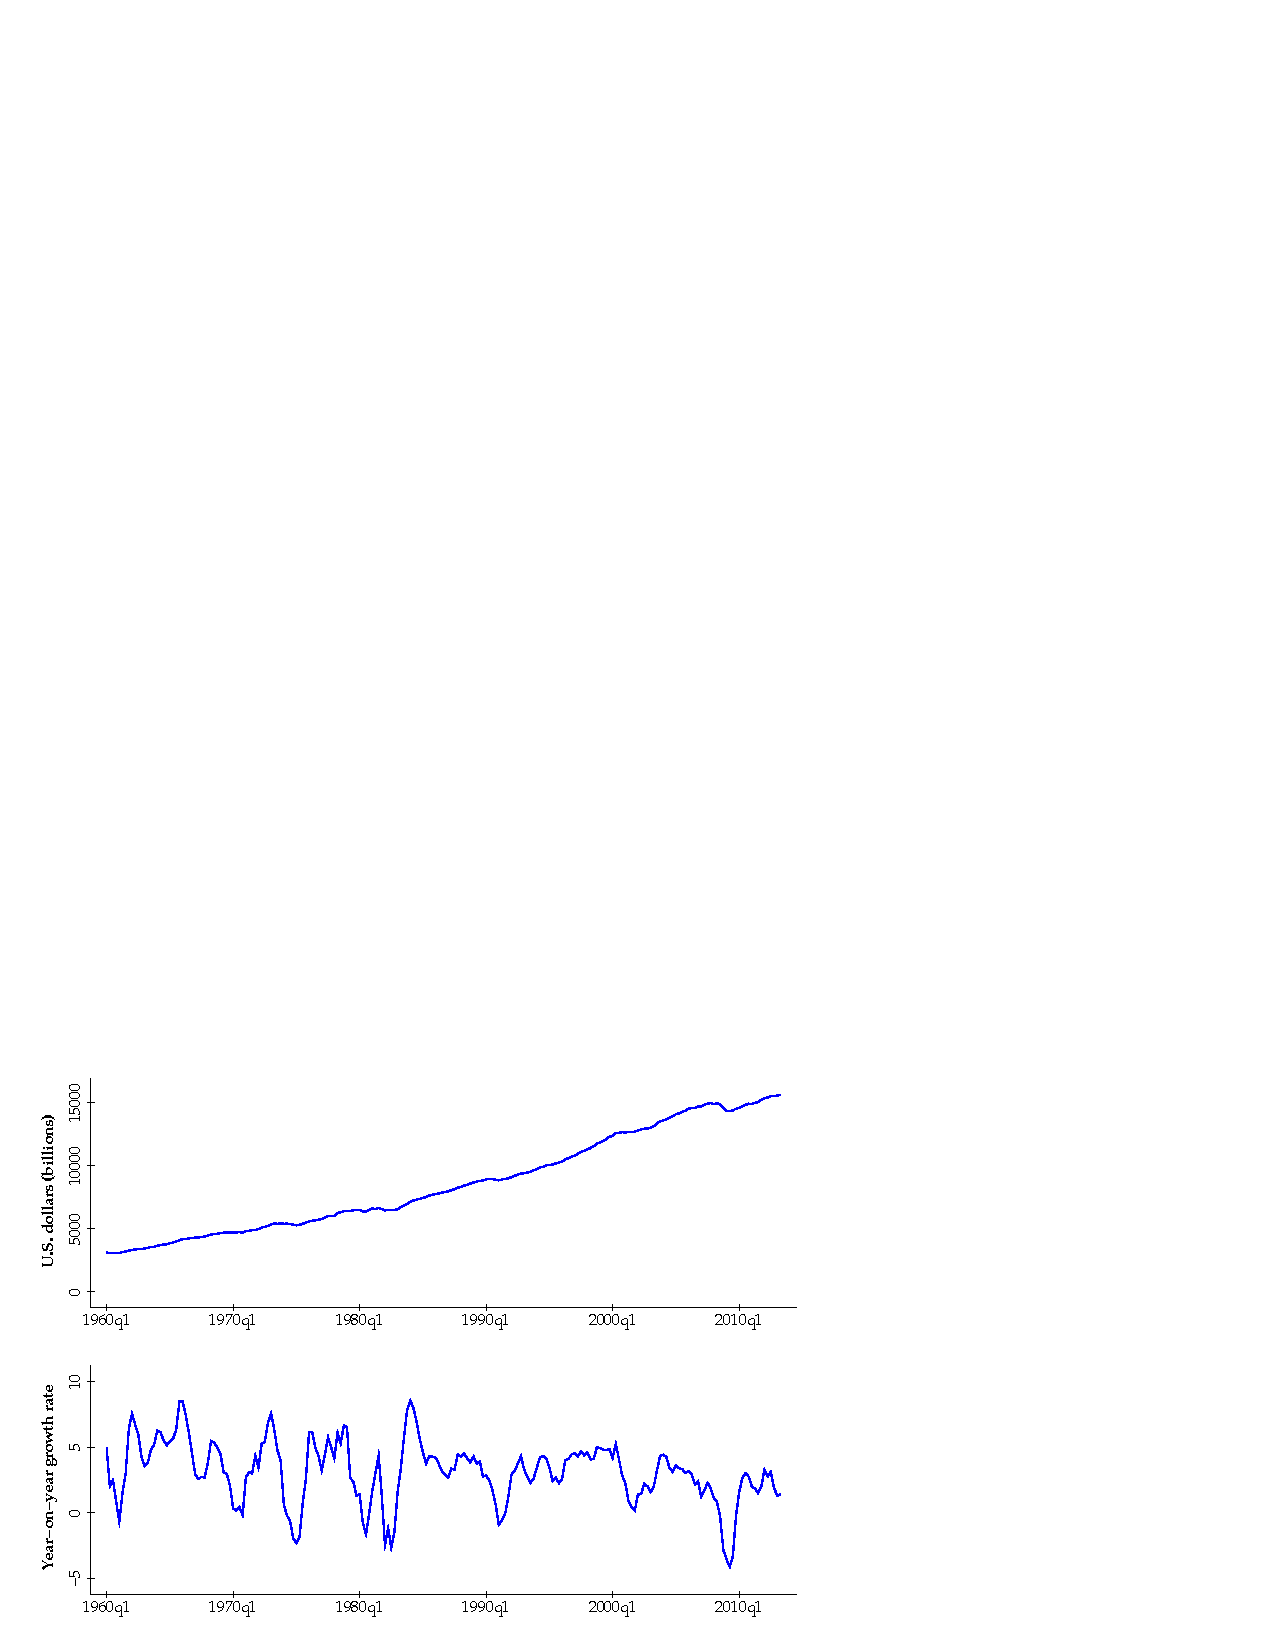
\includegraphics[width=0.8\textwidth]{Figures/us_gdp.pdf}
\end{figure}

The \href{http://www.nber.org/cycles/main.html}{National Bureau of Economic Research},
which dates business cycles in the US,
defines a recession \index{recession} as ``a significant decline
in economic activity spread across the economy,
lasting more than a few months, normally visible in real GDP,
real income, employment, industrial production,
and wholesale-retail sales.''
Using subjective methods, they identify dates of peaks and troughs.
Less formally, many people use the rule of thumb
that a recession consists of two consecutive quarters
in which GDP has fallen.
The year-on-year growth rates in the figure don't coincide exactly
with this definition, but you can see the eight official NBER
recessions since 1960 as sharp downward spikes in GDP growth.


\section{Expenditure components}

Burns and Mitchell refer to fluctuations in
``many economic activities.''
Among these activities are the expenditure
components of GDP.
Are their fluctuations similar to those of GDP?
On the whole, the components, particularly consumption and investment,
move up and down together, but the magnitudes differ enormously.
\href{http://research.stlouisfed.org/fred2/series/PCECC96?cid=110}{Consumption}
currently accounts for about 70 percent of US GDP;
as you might expect, its fluctuations are similar (see Figure \ref{fig:gcall}).
The correlation of year-on-year growth rates in consumption (total)
and GDP is 0.84.\index{gross domestic product (GDP)!real GDP|)}

Table \ref{tab:cycleprops} shows us that consumption's components ---
services, nondurable goods, and durable goods --- also vary with GDP,
but their correlations and (esp) volatilities differ somewhat.
Consumption of nondurables and services
is less volatile than GDP, in the sense that
the standard deviation of its growth rate is smaller.
Consumption of durables is far more
volatile %(in the sense that its standard deviation is larger)
than consumption of nondurables and services.
You might think of specific products and industries that reflect
the same phenomenon.
Why do you think cars and refrigerators
are more volatile than haircuts and medical care?

\begin{table}[h!]
\centering
\caption{Properties of business cycles.}
\label{tab:cycleprops}
\begin{tabular*}{0.8\textwidth}{l@{\extracolsep{\fill}}ccc}
\toprule
        &  Std Dev (\%)  &  Corr w/ GDP  \\
\midrule
GDP     &      2.19          &    1.00      \\
Consumption:  total      &  1.75  &  0.84   \\
Consumption:  services   &  1.22  &  0.63   \\
Consumption:  nondurable &  1.65  &  0.75   \\
Consumption:  durables   &  6.29  &  0.76   \\
Investment:  total       &  6.64  &  0.86   \\
Investment:  structures  &  7.85  &  0.46   \\
Investment:  equipment   &  7.35  &  0.81   \\
Investment:  housing     &  13.05\phantom{1} &  0.60   \\
Employment               &  1.77  &  0.76   \\
S\&P 500 Index           &  14.98\phantom{1}  &  0.36   \\
\bottomrule
\addlinespace
\end{tabular*}
\begin{minipage}{0.8\textwidth}
\footnotesize{Numbers refer to year-on-year growth rates computed from quarterly US data.}
\end{minipage}
\end{table}

\begin{figure}[h!]
    \caption{Fluctuations in consumption, investment, and GDP.}
    \label{fig:gcall}%
    \centering
    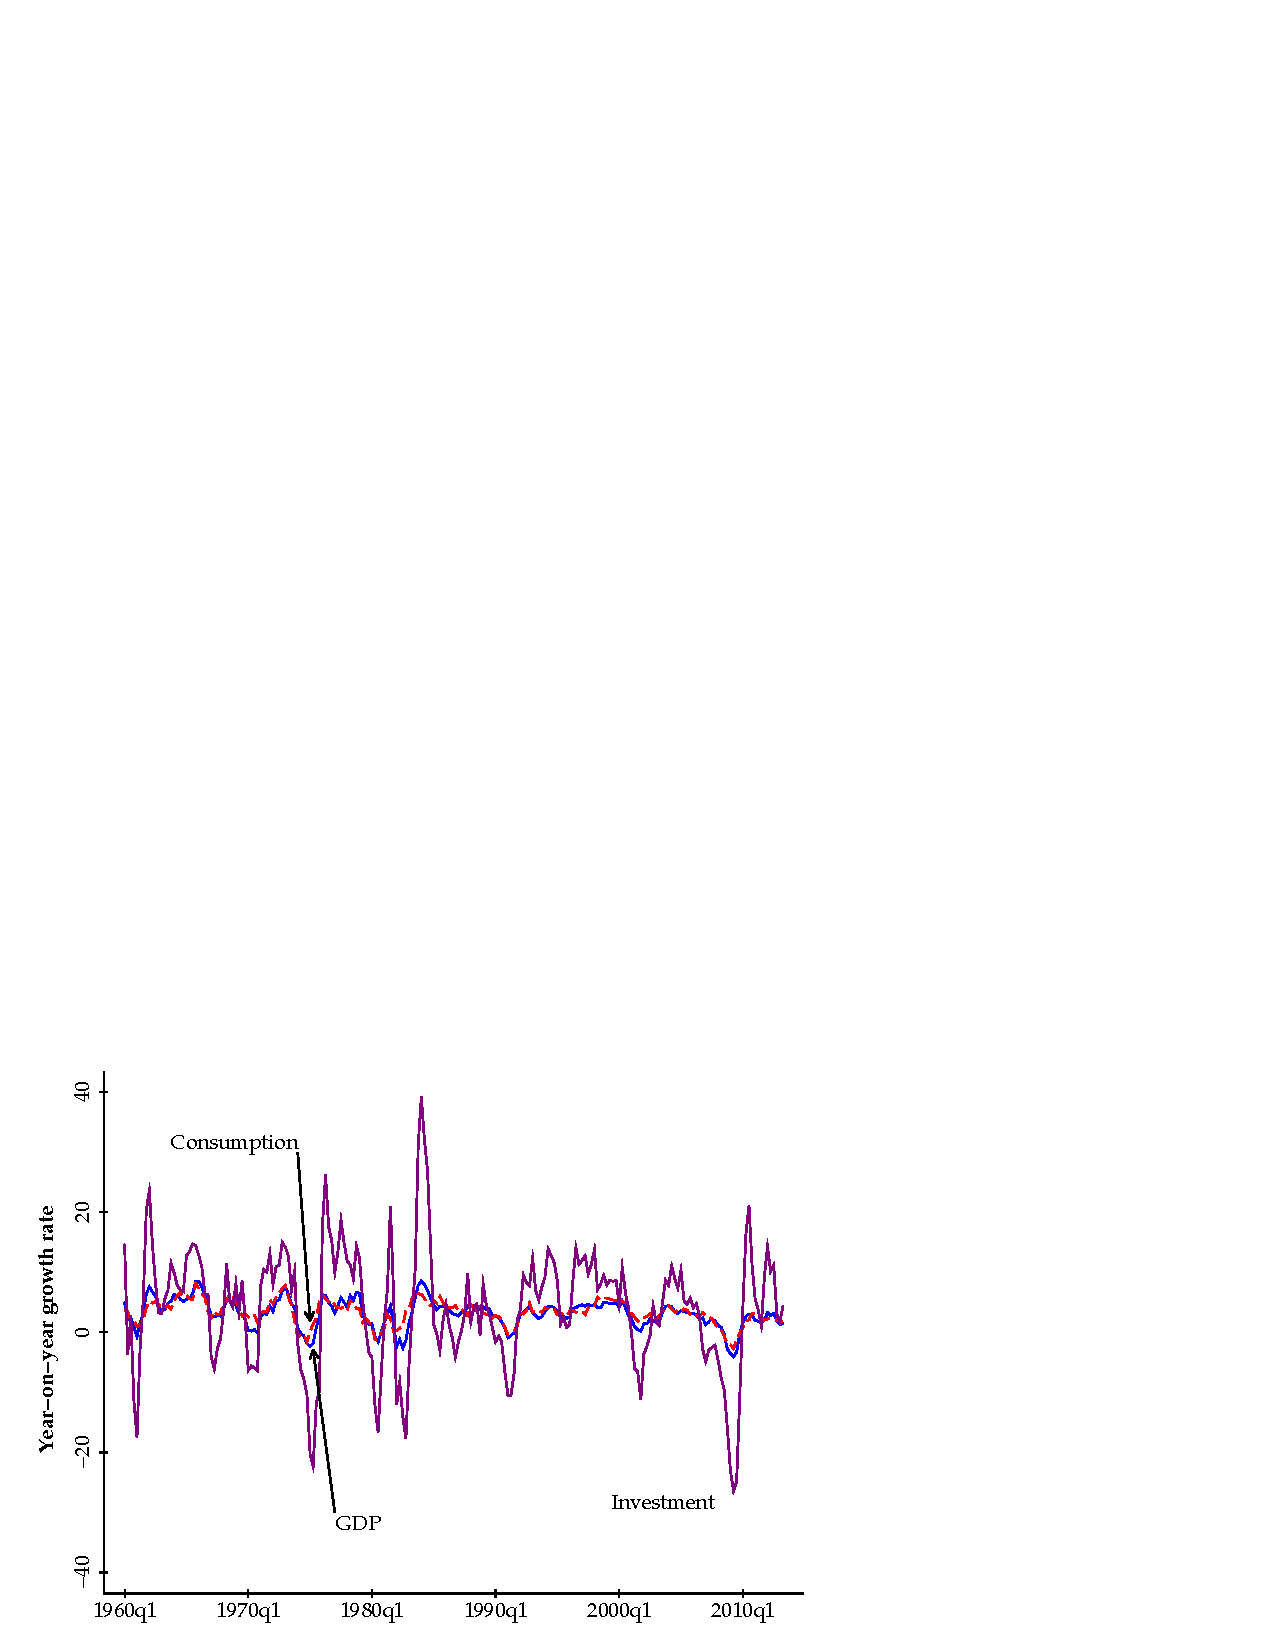
\includegraphics[width=0.8\textwidth]{Figures/us_inv_cons_gdp.pdf}
\end{figure}

\href{http://research.stlouisfed.org/fred2/series/GPDIC96?cid=112}{Investment}
also moves up and down with output
and is substantially more volatile (see Figure \ref{fig:gcall}).
As a rule of thumb, a one-percent increase in GDP is associated with
about a three-percent increase in total investment.
(We're looking at the ratio of standard deviations here,
and the high correlation of the two series.)
Table \ref{tab:cycleprops}
shows that the major components of investment --- structures, equipment,
and residential housing --- are highly correlated with,
and more volatile than, GDP.


When we turn to \index{cyclical indicators}
business-cycle indicators, we'll see that
many of them are more detailed measures of
some aspect of consumption or investment.
Consumption is important because it accounts for most of GDP.
Investment is important because it is highly responsive
to changes in economic conditions.


\section{Labor and capital markets move with the cycle}

Labor markets also move with the business cycle;
indeed, it's the way in which business cycles make themselves
known to us most directly.
Figure~\ref{fig:labor} shows us how fluctuations in
\href{http://research.stlouisfed.org/fred2/series/PAYEMS}{employment}
covary with GDP.
Note that employment growth is generally less than GDP growth;
the difference reflects an increase in output per worker --- a good thing, to be sure!
You can see in the figure that the ups and downs in employment
typically lag those in GDP by a little --- a quarter or two.
The current expansion is an extreme case, with
GDP rebounding well before employment,
but the general pattern is not unusual.

\begin{figure}[h!]
\caption{Fluctuations in employment and GDP.}
    \label{fig:labor}%
    \centering
    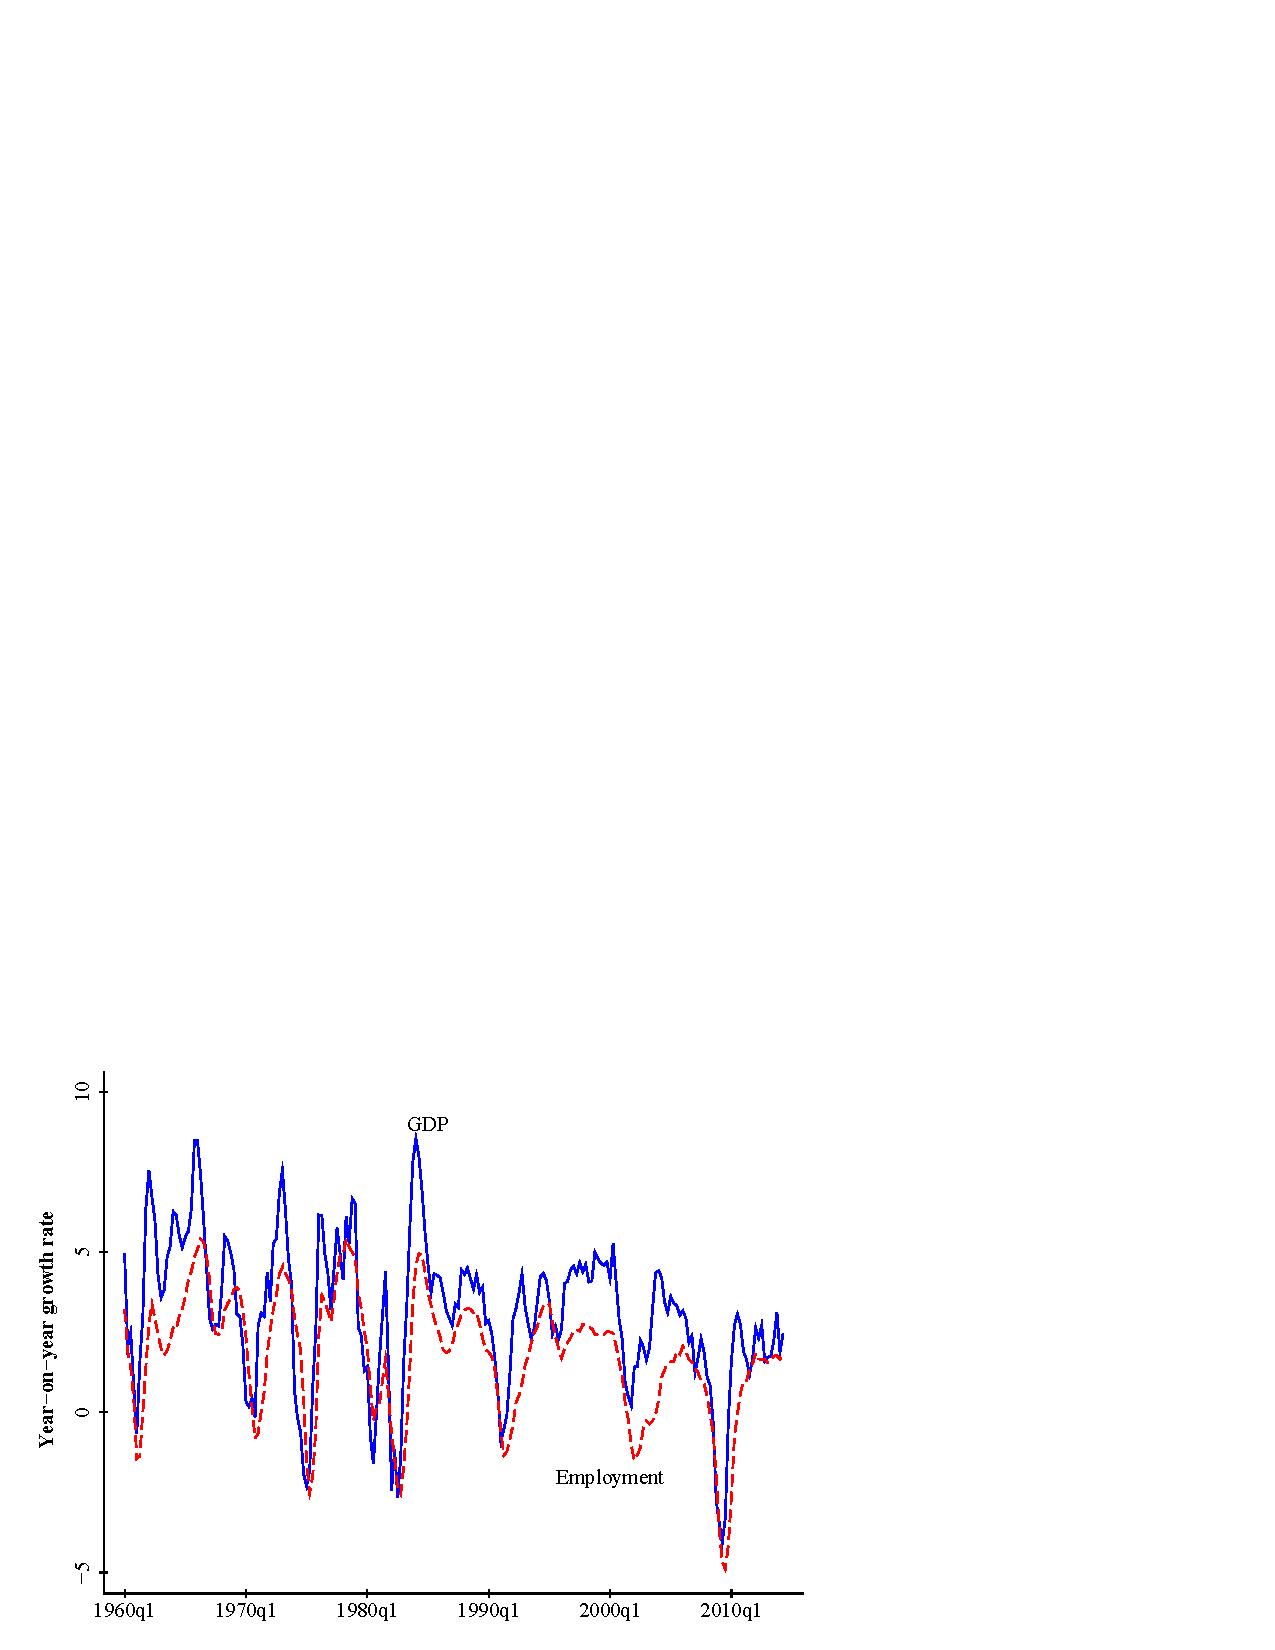
\includegraphics[width=0.8\textwidth]{Figures/us_emp_gdp.pdf}
\end{figure}

\begin{figure}[h!]
    \caption{Fluctuations in asset prices and GDP.}
    \label{fig:stock}%
    \centering
    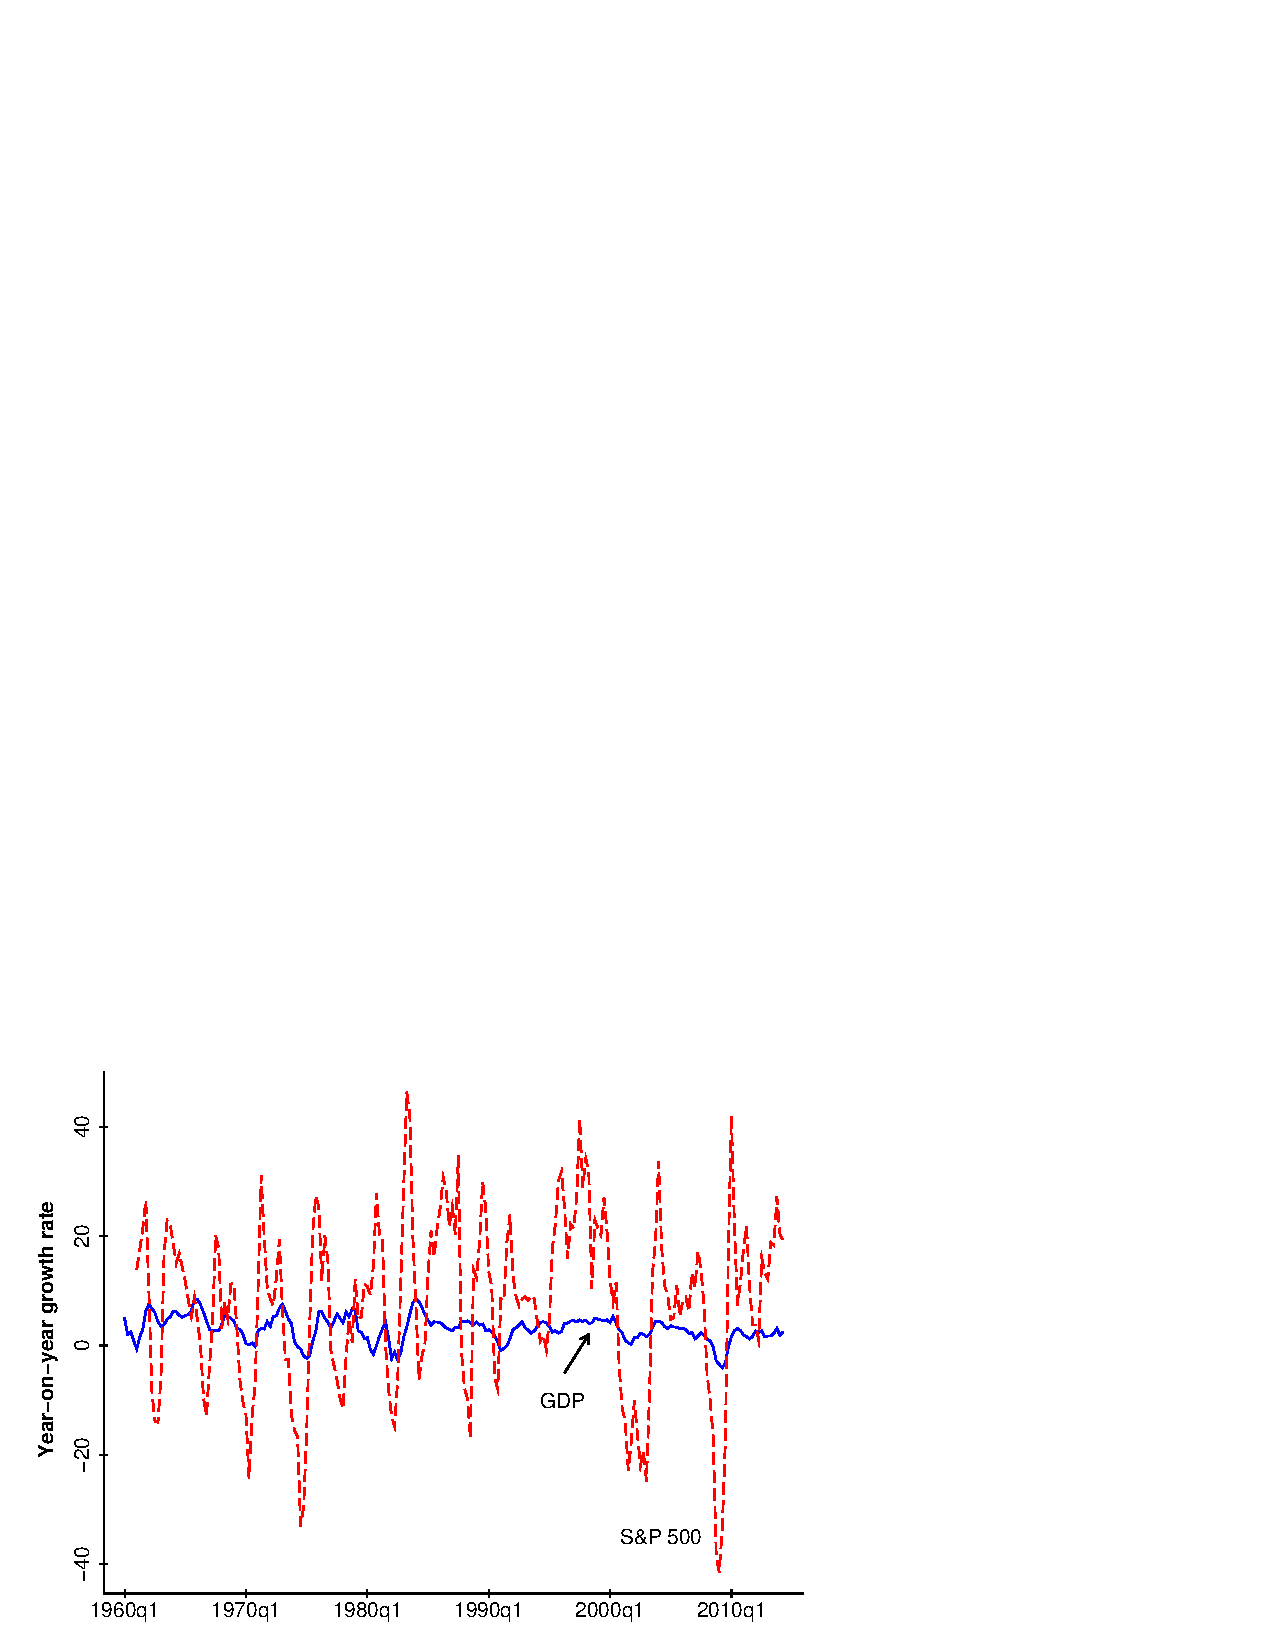
\includegraphics[width=0.8\textwidth]{Figures/us_gdp_sp500.pdf}
\end{figure}

Financial (capital) markets move with the business cycle, as well. Figure \ref{fig:stock} plots the growth rate of real GDP\index{gross domestic product (GDP)!real GDP} against versus the yearly growth rate of the \href{http://research.stlouisfed.org/fred2/series/SP500}{S\&P 500 index}. Notice that aggregate stock prices are extremely volatile, with a standard deviation about eight times larger than GDP. Moreover, aggregate stock prices and GDP are positively correlated (0.36). This suggests that good news about the economy is good news for stock prices.
It's hard to see in Figure \ref{fig:stock},
but we'll see later that stock prices lead GDP;
the correlation of stock prices with GDP two quarters later is above 0.5. Financial
measures often lead economic activity. Another example is the yield \index{bond!bond yield}
 curve (the difference
between long-term and short-term interest rates),
which tends to flatten or invert ahead of business downturns.
We'll look at this more closely when we turn to indicators.


Labor markets and asset prices are
both sources of useful indicators of economic activity.
We'll see more of each shortly.


\section*{Executive summary}

\setlength{\leftmargini}{.5\oldleftmargini}
\begin{enumerate}
\item Economies do not grow smoothly; they exhibit lots of
short-term volatility.

\item Spending on investment goods (by firms)
and consumer durables (by households) are more volatile
 than output as a whole.
 Household spending on nondurable goods and services
 is less volatile than output.

\item Most variables are procyclical\index{business cycle!procyclical}; that is, they move up and down with GDP.
Examples include consumption, investment, employment, and the stock market.
\end{enumerate}
\setlength{\leftmargini}{\oldleftmargini}

\section*{Review questions}

\setlength{\leftmargini}{.5\oldleftmargini}
\begin{enumerate}
\item Statistics.  What statistic would you use to show that two economic series
move up and down together?

Answer.  The correlation between them.
Table \ref{tab:cycleprops}, for example, includes the correlations
of year-on-year growth rates of GDP and several expenditure components.
The correlations in most cases are above 0.8, indicating they do indeed
mostly move up and down together.

\item More statistics.  What statistic would you use
 to show that one series is more ``volatile''
than another.

Answer.  The standard deviation.
In the same table, we saw that investment is more volatile than consumption
in the sense that its standard deviation is about three times higher.

\item Do it yourself.  Reproduce Figure \ref{fig:labor} in FRED.
The variables are real GDP (FRED code GDPC1) and nonfarm employment
(PAYEMS).
\end{enumerate}
\setlength{\leftmargini}{\oldleftmargini}

\section*{If you're looking for more}

These basic features of business cycles \index{business cycle|)}
 are covered in most
macroeconomics textbooks.
A reasonably good overview is Finn Kydland and Edward Prescott,
``\href{http://www.minneapolisfed.org/publications_papers/pub_display.cfm?id=225}
{Real facts and a monetary myth}.''

\section*{Data used in this chapter}

\begin{table}[H]
\centering
\caption{Data table.}
\begin{tabular*}{0.8\textwidth}{l@{\extracolsep{\fill}}l}
\toprule
Variable & Source\\
\midrule
GDP                            &GDPC1\\
Consumption                    &PCECC96 \\
\hspace{0.2in}Services        &PCESVC96\\
\hspace{0.2in}Durables        &PCDGCC96\\
\hspace{0.2in}Nondurables    &PCNDGC96\\
Investment                    &GPDIC96\\
\hspace{0.2in}Nonresidential &PNFIC96\\
\hspace{0.4in}Equipment        &NRIPDC96\\
\hspace{0.2in}Housing        &PRFIC96\\
Employment                    &PAYEMS\\
S\&P500                     &SP500\\
10yr Treasury yield \index{bond!bond yield}
            &GS10\\
2yr Treasury yield \index{bond!bond yield}
            &GS2\\
Federal funds rate            &FEDFUNDS\\
\bottomrule
\addlinespace
\end{tabular*}
\begin{minipage}{0.8\textwidth}
\footnotesize{To retrieve the data online, add the identifier from the source column to \url{http://research.stlouisfed.org/fred2/series/}.  For example, to retrieve nonfarm employment, point your browser to \url{http://research.stlouisfed.org/fred2/series/PAYEMS}}
\end{minipage}
\end{table}

\chapter{Business-Cycle Indicators}
\label{chp:bcin}
\hypertarget{indicators}{}

%No extra line here.
\textbf{Tools:} Basic statistics (standard deviation, correlation); cross-correlation function.

\textbf{Key Words:} Volatility; procyclical and countercyclical; leading, lagging, and coincident.

\needspace{4\baselineskip}
%\textbf{Big Ideas:}
\vspace{-0.1in}
\begin{itemize}
    \item Business cycle indicators are characterized by several properties:  procyclical and   countercyclical, leading and lagging.
    \item Cross-correlation functions identify these properties.
\end{itemize}

\rule{\textwidth}{1pt}

Probably the leading use of macroeconomic data (and macroeconomists)
is forecasting:  predicting future movements in economic variables
so that businesses can decide how much to produce,
investors can decide how to allocate their assets,
and households can decide how much to spend.
The good news is that forecasting is possible;
we're not simply throwing darts at a board.
The bad news is that it's not easy;
even the best forecasters are far from perfect.

This chapter is devoted to short-term business-cycle
indicators --- variables that indicate changes in near-term economic conditions --- and how to use them.
In principle, we could be interested in many features of
the economy:  output, inflation, interest rates,\index{inflation}
exchange rates, and so on.
We'll focus on output, but the methods can easily be applied
to other variables.
We look at the US, but similar ideas and methods apply to
any country with reliable data.


\section{Terminology}

We refer to the properties of economic indicators with two related sets of terms.
One set of terms
describes whether an indicator's movements
tend to come before or after movements in output.
We say an indicator {\it leads\/} \index{cyclical indicators!leading indicator} output if
its ups and downs typically precede those of output,
and {\it lags\/} \index{cyclical indicators!lagging indicator} output if they come after.
An indicator whose movements are contemporaneous with those of output
is referred to as {\it coincident\/}. \index{cyclical indicators!coincident indicator}
Thus, the adjectives leading, lagging, and  coincident
describe the timing of an indicator's movements relative to those of output.
Looking ahead, you might guess that leading indicators are
most useful in forecasting.
The stock market, for example, is a common leading indicator;
it leads output by six to eight months, as we'll see shortly.


A second set of terms refers to
whether an indicator's movements
are positively or negatively correlated with output.
If the correlation is positive, we say it is {\it procyclical\/};
if the correlation is negative, we say it is {\it countercyclical\index{business cycle!countercyclical|textbf}
\/}.
%If its movements are unrelated to those in output,
%we say it is {\it acyclical\/}.
Most indicators are procyclical\index{business cycle!procyclical|textbf}:  employment, stock prices, \
housing starts, and so on.
The most common   countercyclical   \index{business cycle!countercyclical}
 indicators have to do with unemployment: Both the unemployment rate and new claims for unemployment insurance
 rise during recessions.

\section{Forecasting \index{forecasting}}

The classic forecasting problem goes something like this:
What do we expect the value of [some
economic variable] to be $k$ periods in the future?
Here, $k$ is any period of time you like, but
we're usually interested in anything from next week to a few years in
the future.\index{industrial production|(}

\begin{figure}
    \caption{US GDP and industrial production.}
    \label{fig:ip_gdp}%
    \centering
    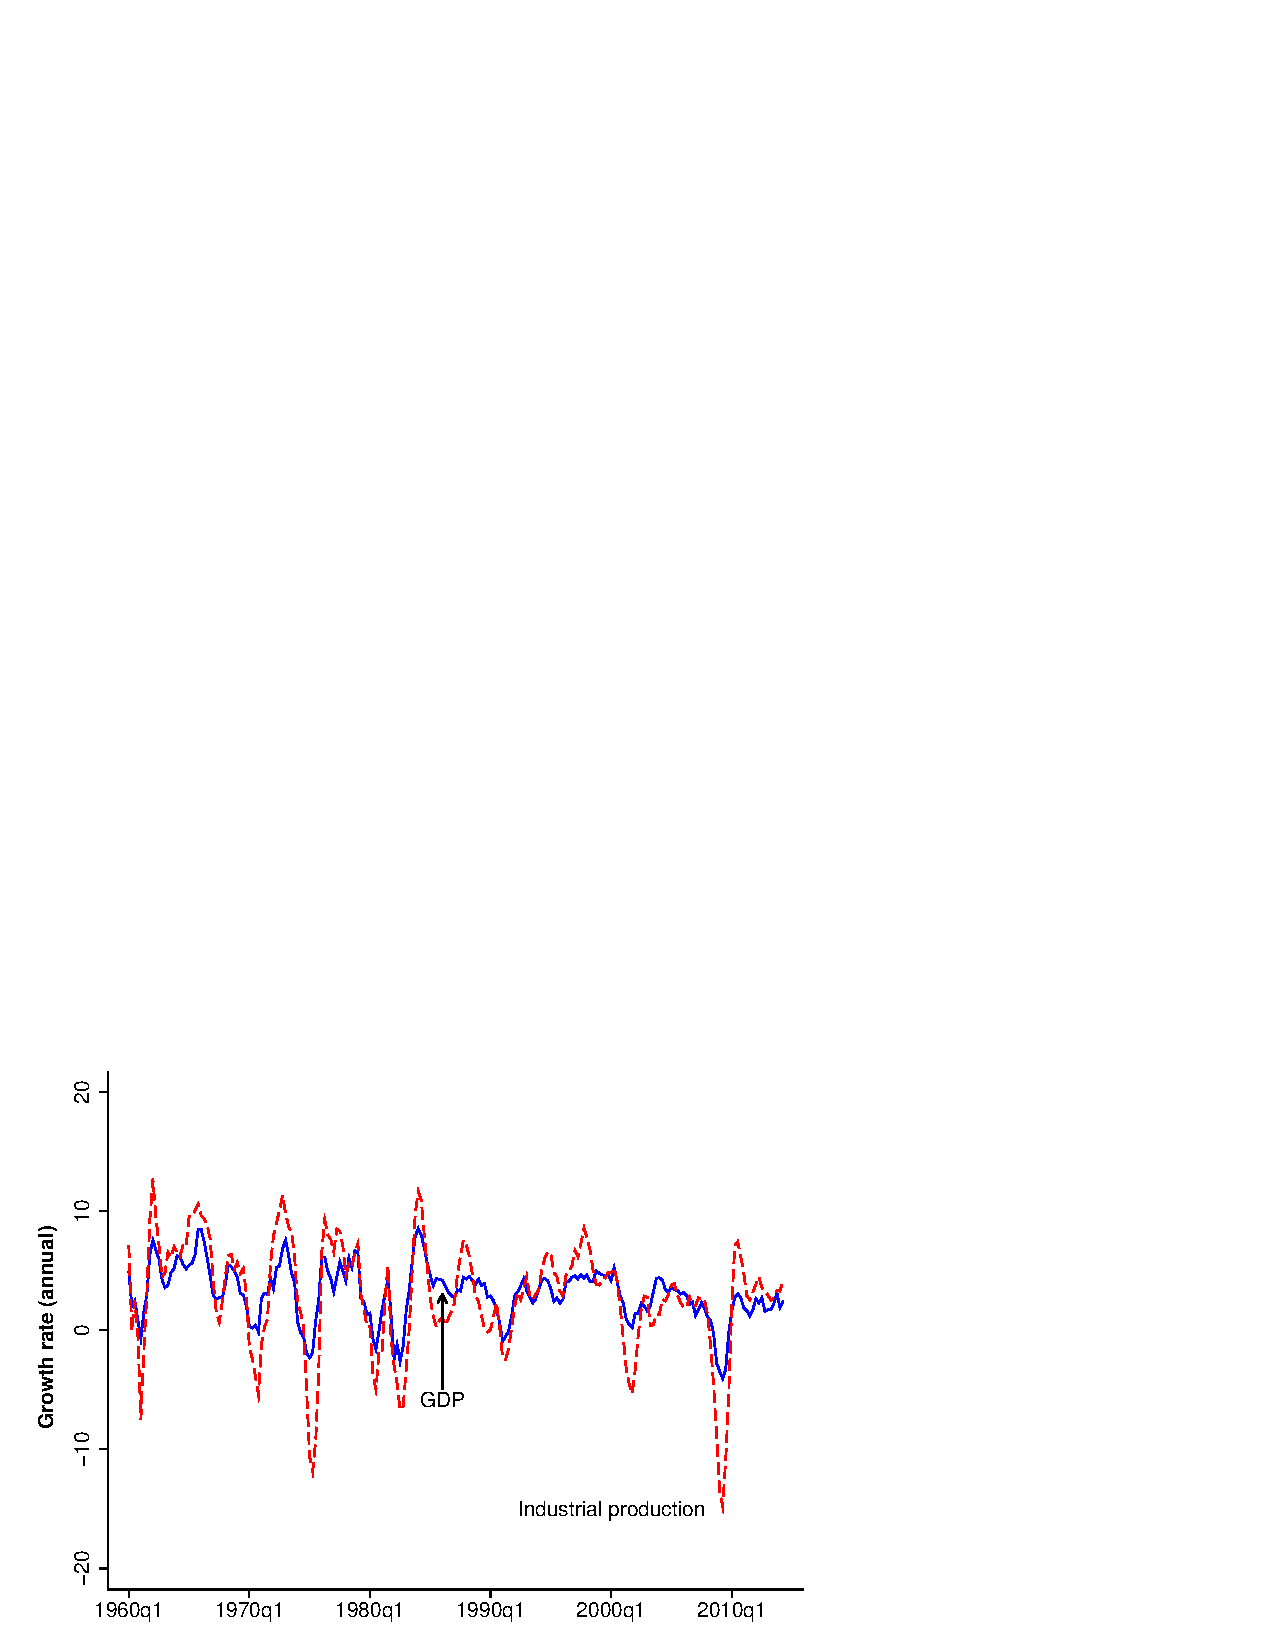
\includegraphics[width=0.8\textwidth]{\figpath Figures/us_gdp_indprod.pdf}
\end{figure}


If we're forecasting GDP, there's an extra difficulty because we don't
know the present or the recent past, much less the future. We've
seen, for example, that fourth-quarter GDP is first reported near
the end of the following January, and even that number is a
preliminary estimate. From the perspective of mid-January, then,
we need to ``forecast'' the previous quarter.\index{gross domestic product (GDP)!real GDP}


We're going to shortcut this difficulty (somewhat) by using the
monthly \href{http://research.stlouisfed.org/fred2/series/INDPRO?cid=3}{Industrial Production (IP)} index as a substitute for real
GDP, but the issue is a general one, in that the time lag in getting data
is both an issue in its own right and a  constraint on forecasting
the future. IP measures output in manufacturing, mining, and
utilities. More important, its fluctuations are strongly
correlated with those in GDP.  You can see that in
Figure~\ref{fig:ip_gdp}, which compares year-on-year growth rates
in GDP and IP (aggregated to a quarterly frequency). You will
notice that IP is more volatile than GDP but otherwise follows its
ups and downs reasonably well.  You may also notice some
differences between them in the recent past, which have been
traced to the rising importance of services in the US economy.  In
the US, IP is reported by the Federal Reserve in the middle of the
following month.  Data for December, for example, are available in
mid-January.  Using IP, therefore, gives us a shorter information
lag than GDP.  In addition, the monthly frequency gives us a finer
time interval for near-term forecasting.  For both reasons, we
will focus our discussion of forecasting on IP rather than, GDP,
although the same principles apply to both, as well as to other
macroeconomic and financial variables.\index{industrial production|)}

\section{Good indicators}

Good forecasts require good inputs.
One way to forecast a variable is with its own past.
Future growth rates of IP, for example, might be related
to current and past growth rates.
We can usually do better than that by adding other indicators
to our analysis.
Speaking generally,
a good indicator should have one or more of these properties:
%
\begin{itemize}

\item \textbf{Correlation.}  A good indicator is correlated with the
variable we are forecasting.

\item \textbf{Lead.} A good indicator leads the variable we are
forecasting.

\item \textbf{Timeliness.}  A good indicator is available quickly.

\item\textbf{Stability.}  A good indicator does not undergo major
revisions subsequent to its initial release, and its
relationship with the variable we are forecasting doesn't
change over time.

\end{itemize}
On the whole, measures of economic activity
(employment, for example)
tend to be strong on correlation and weak on timeliness (see the
discussion of GDP above) and stability (many economic series are
revised frequently).  The best ones lead the business cycle.  In
contrast, financial indicators (equity prices, interest rates) are
weaker on correlation but stronger on the other three properties:
They're typically available immediately, often lead the cycle, and
are not revised.
Various indexes of leading indicators combine multiple series with the
hope of getting the best from each.  The Conference Board's
quasi-official index of leading indicators is the most common example.



\section{Identifying good indicators}

How do we identify indicators with high potential?
We'll use another bit of terminology that leads to an extremely useful
graphical representation of the dynamic relation between two variables:
the {\it cross-correlation function\/} (ccf).\index{cross-correlation function|(}

You may recall that the correlation between two variables
($x$ and $y$, say) is a measure of
how closely they are related in a statistical sense.
If the correlation is (say) 0.8,
then observations with large values of $x$
tend also to have large values of $y$.
If the correlation is 0.4, this association is weaker.
And if the correlation is --0.8,
observations with large values of $x$
tend to have small values of $y$ --- and vice versa.

\begin{figure}[!ht]
    \caption{Cross-correlations: the S\&P 500 and industrial production.}
    \label{fig:ccf-sp500}%
    \centering
    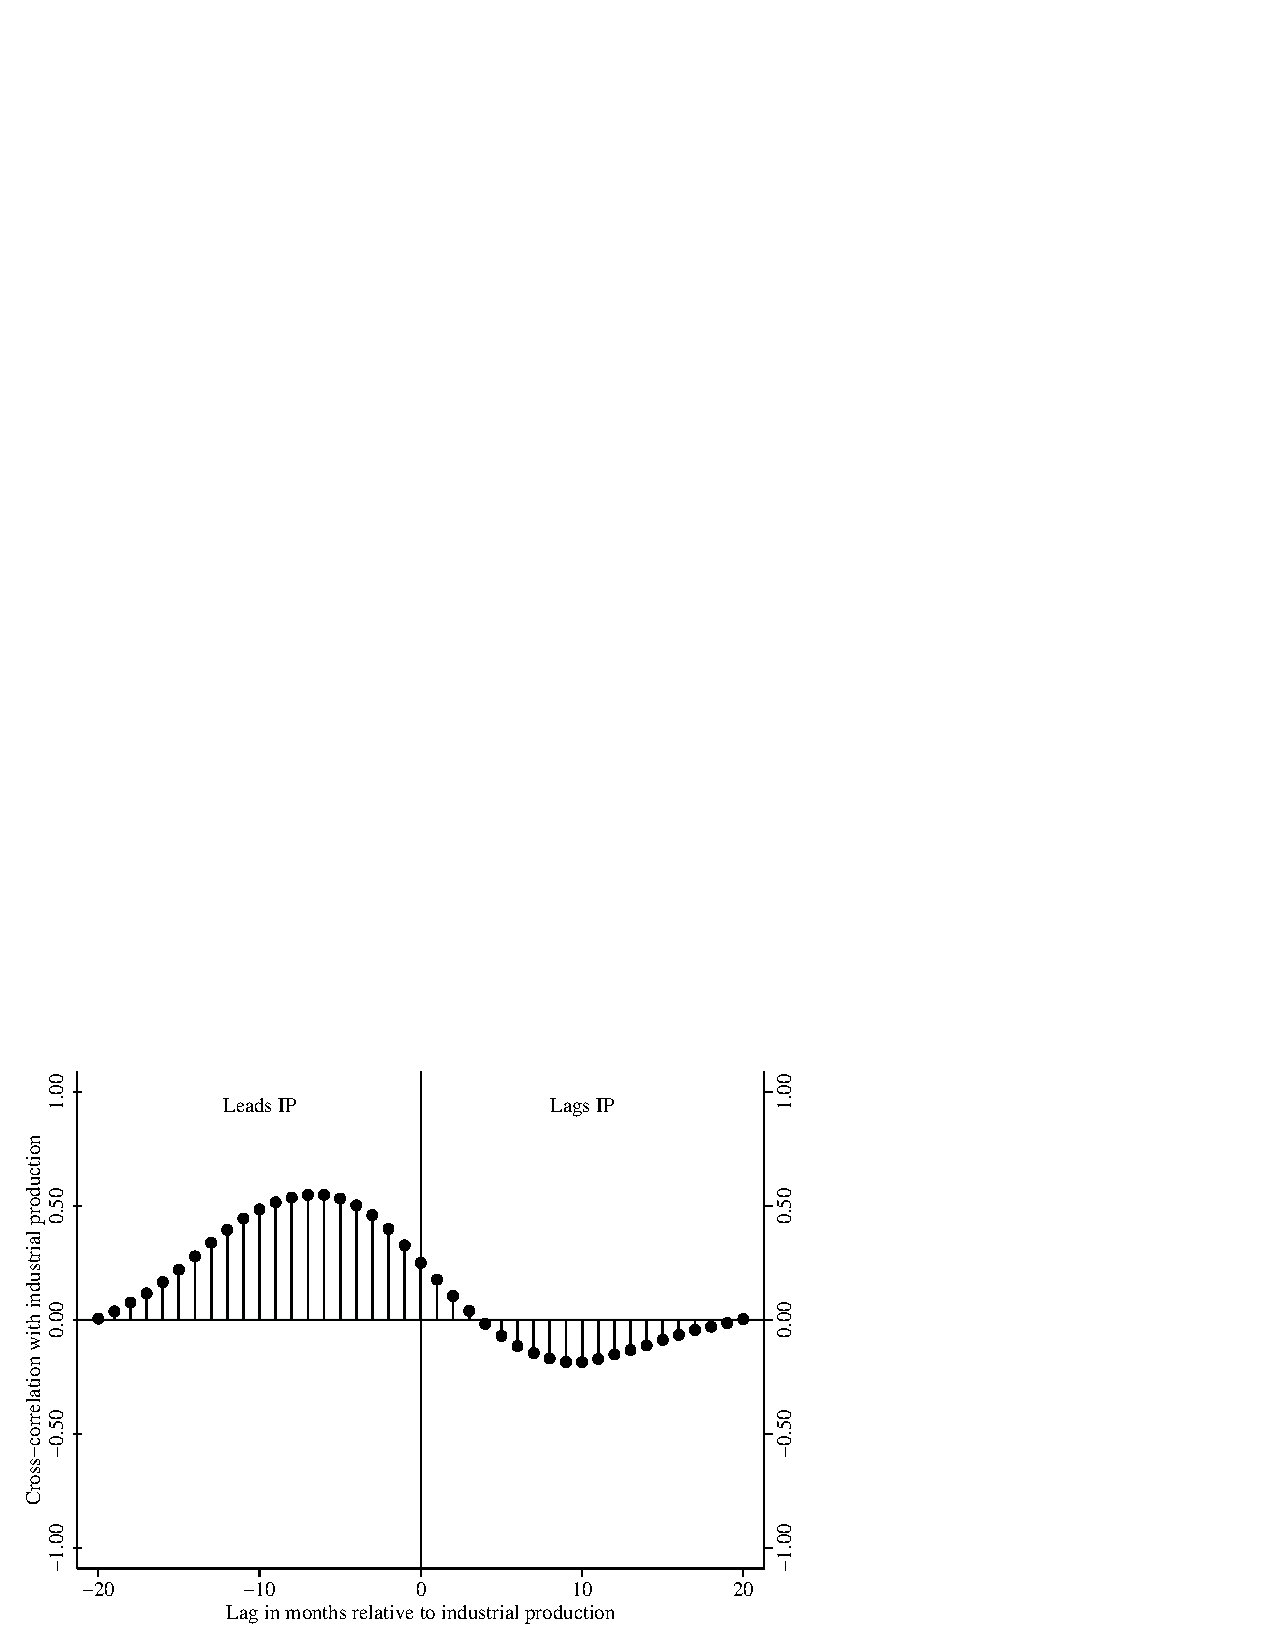
\includegraphics[width=0.8\textwidth]{\figpath Figures/xcsp500.pdf}

    \begin{minipage}{0.8\textwidth}
    \footnotesize{Both series are year-on-year growth rates for the period
    1960-present.
    The large correlations to the left tell us that
    the S\&P 500 index is a good indicator of future industrial production.}
    \end{minipage}
\end{figure}

The cross-correlation function extends the concept of correlation
to the timing of two indicators.
Specifically, consider the correlation between $x$ at date $t$
and $y$ at date $t-k$.  If $k$ is negative,
then we're talking about the correlation
between $x$ now and $y$ $k$ periods in the future.
If $k$ is positive, we have the correlation between $x$ now and
$y$ $k$ periods in the past.
By looking at the pattern of correlations,
we can identify indicators $x$ that tend to lead the variable $y$.
We refer to $k$ as the lag of $y$ vs $x$,
but if $k$ is negative it refers to a lead.
Mathematically, we write
\[
    \mbox{ccf}(k) \;=\;  \mbox{\it corr\/} (x_t,y_{t-k}) .
\]
Typically, we would graph this against $k$, with $k$ starting
with a negative number and moving to positive numbers.
The pattern of correlations tells us whether an indicator $x$
leads or lags (on average) a variable $y$.


Let's move from the abstract to the concrete to make sure we
understand what the ccf represents.\index{industrial production|(}
[You might want to work your way through this paragraph slowly,
it's important.]
We calculate the year-on-year growth rates of the \href{http://research.stlouisfed.org/fred2/series/SP500}{S\&P 500 index}
and industrial production and compute their ccf using
the S\&P 500 for $x$ and industrial production for $y$.
Figure \ref{fig:ccf-sp500} is a plot of their correlations against
the lag $k$.
There's a lot of information here, so let's go through it
one dot at a time.
The dot at $k=0$ (on the vertical line at the center of the figure)
shows that the contemporaneous correlation is about 0.2.
Contemporaneous means that we're looking at the two variables
at the same time:
March 2001 industrial production is lined up with March 2001 S\&P 500,
and so on.
Next, consider the dot corresponding to $ k = -10$ on the left
side of the figure.
The correlation of (roughly) 0.5 pictured in the figure
shows the growth rate of industrial production with
the growth rate of the S\&P 500 index dated
ten months earlier.
Evidently high growth in equity prices now
is associated with high growth in IP 10 months later.
Finally, consider a dot on the right side of the figure.
The dot at $k=+10$ suggests that the correlation
of industrial production growth with equity price growth tex months
later is about --0.2.

This pattern of correlations tells us a lot about the
timing of movements in the two variables.
In general, negative values of $k$ (the left side of the figure)
indicate correlations of the S\&P 500 with
future industrial production; we would say that they reflect the tendency
of stock prices to lead output.
Positive values of $k$ (the right side of the figure)
indicate correlations of the S\&P 500 with
past industrial production; they reflect
the tendency of stock prices to lag output.
What we see in the figure is a strong correlation of the S\&P 500 index
with industrial production seven to eight months later.
Evidently, the stock-price index is a leading indicator of
industrial production. \index{industrial production (IP)}

We'll use the cross-correlation function to identify whether
an indicator is leading or lagging, procyclical \index{business cycle!procyclical}
 or   countercyclical.   \index{business cycle!countercyclical}

To do this, we find the largest correlation in absolute value.
If it occurs to the left of the figure, we say it's a leading indicator;
if on the right, lagging.
Similarly, if the (largest) correlation is positive,
we say the indicator is procyclical\index{business cycle!procyclical};
if negative,   countercyclical\index{business cycle!countercyclical}.
In principle an indicator could be both leading and lagging,
or both pro- and counter-cyclical,
but we'll deal with that if and when it happens.

Digression.
{\footnotesize We snuck something in here that we
should mention again,
although it's not particularly important for our purposes.
We used year-on-year growth rates instead of monthly
growth rates.
We could use either, but the year-on-year pictures are smoother
and, in our view, more attractive.
We'd see a similar pattern with monthly growth rates, but the correlations would be both smaller and choppier. }


Let's look at some other indicators and see which ones lead IP.
Some of the most common indicators are labor-market variables,
constructed by the Bureau of Labor Statistics.
Cross-correlation functions for four of them are pictured in
Figure \ref{fig:ccf-labor}.
\href{http://research.stlouisfed.org/fred2/series/PAYEMS}{Nonfarm payroll employment} (a measure of employment constructed
from a survey of firm payrolls) is a slightly
lagging indicator since the ccf peaks with a lag of one to two months.
It is, nevertheless, useful because the correlation (over 0.8) is
unusually strong.
And even a two-month lag is more timely than the GDP numbers.
The unemployment rate is   countercyclical   \index{business cycle!countercyclical}
 (note the negative correlations)
and lags IP in the sense that the largest correlation comes at a
lag of three to four months.
It seems that a rise (fall) in output is associated with a fall (rise)
in the unemployment rate three to four months later.
%Moreover, the lag decays slowly.
%What we're picking up here is that unemployment rises during recessions,
%but declines slowly after the economy recovers.
\href{http://research.stlouisfed.org/fred2/series/IC4WSA}{New applications (``claims'') for unemployment insurance} are also
  countercyclical\index{business cycle!countercyclical}, but the correlation is stronger than for
the overall unemployment rate, and it leads
industrial production by two to three months.
Another popular indicator
is \href{http://research.stlouisfed.org/fred2/series/AWHMAN}{average hours worked per week in manufacturing}.
This indicator is strongly procyclical \index{business cycle!procyclical}
 and leads industrial production
by two to four months.
The labor market, in short, provides a good overall picture of the
economy and, in some cases, supplies indications of future movements
in industrial production.
The leading variables (``new claims'' and ``average weekly hours'')
are more highly correlated with industrial production
than the S\&P 500 index, but the leads are shorter.

\begin{figure}
    \caption{Cross-correlation functions:  labor market indicators.}
    \label{fig:ccf-labor}%
    \centering
    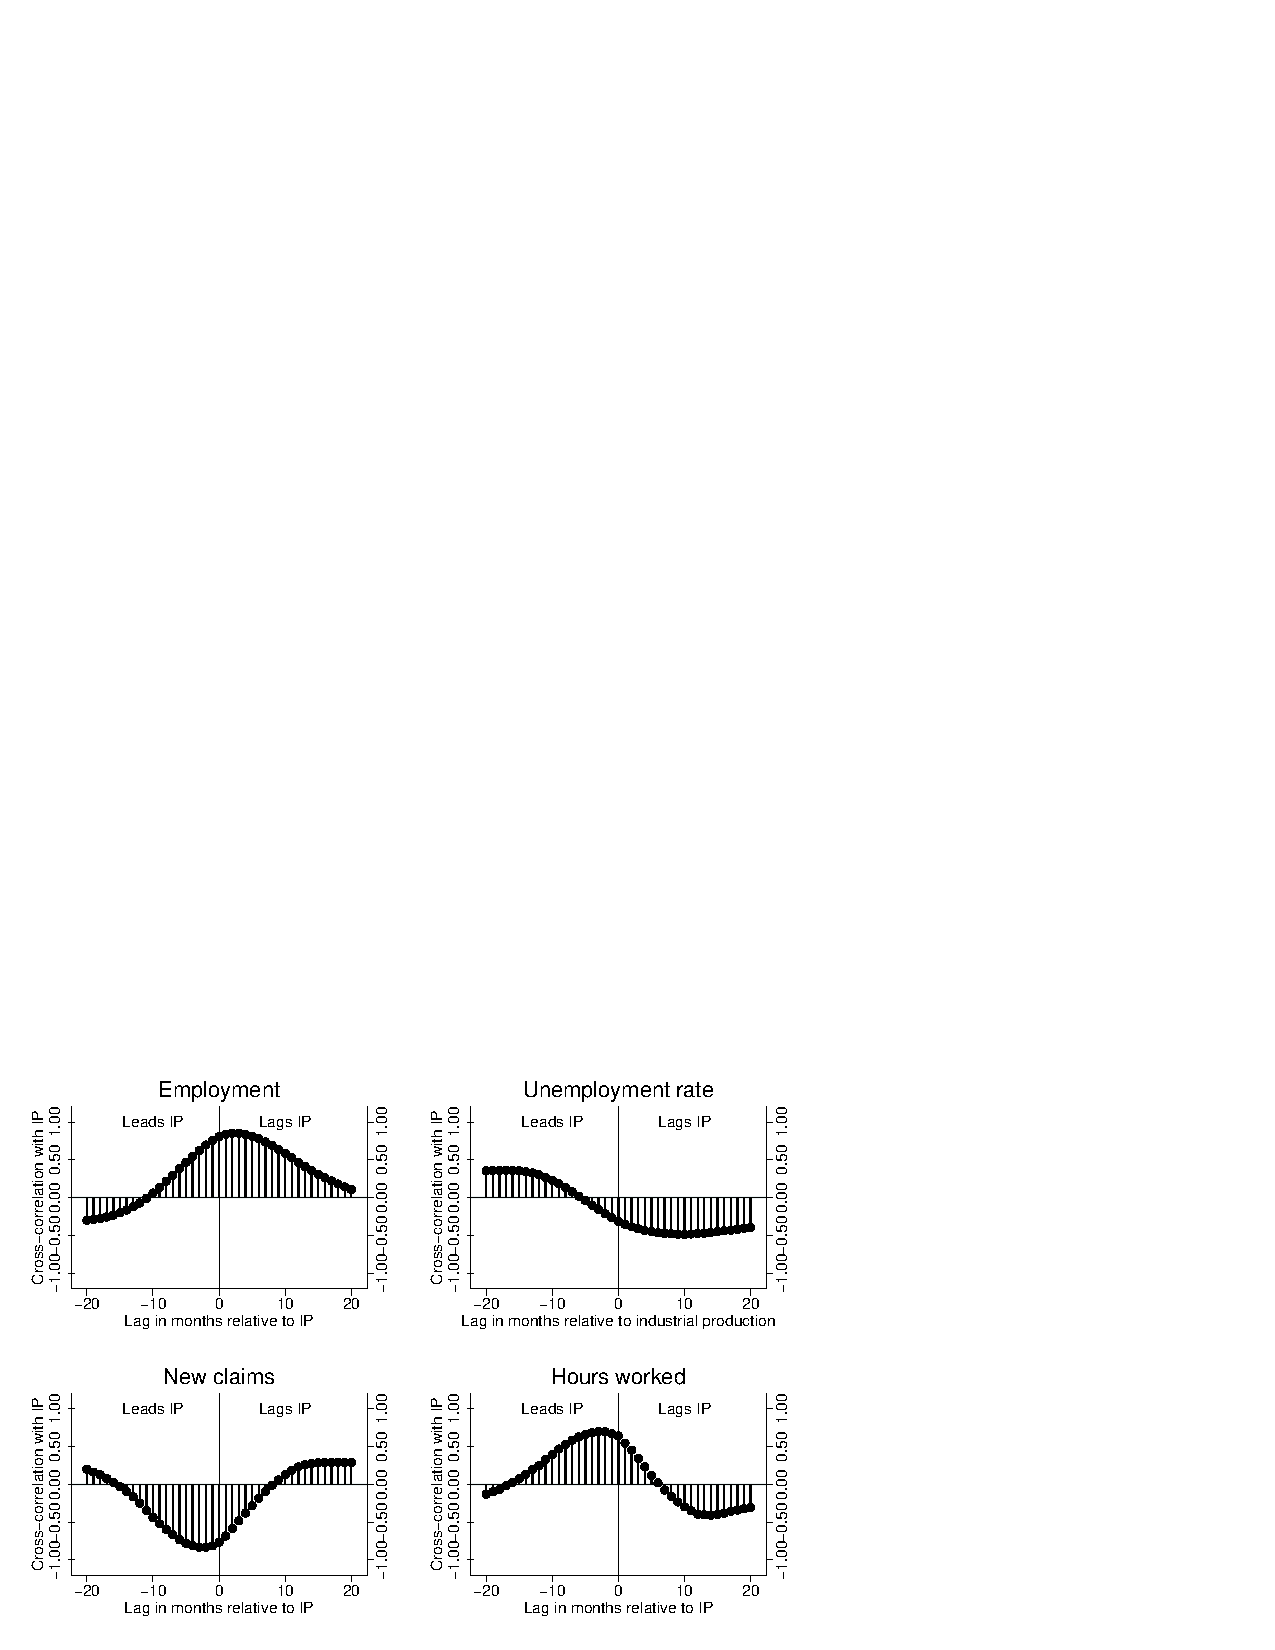
\includegraphics[width=0.9\textwidth]{\figpath Figures/xclabor.pdf}
\end{figure}

\begin{figure}
     \caption{Cross-correlation functions:  surveys of economic activity.}
    \label{fig:ccf-survey}%
    \centering
    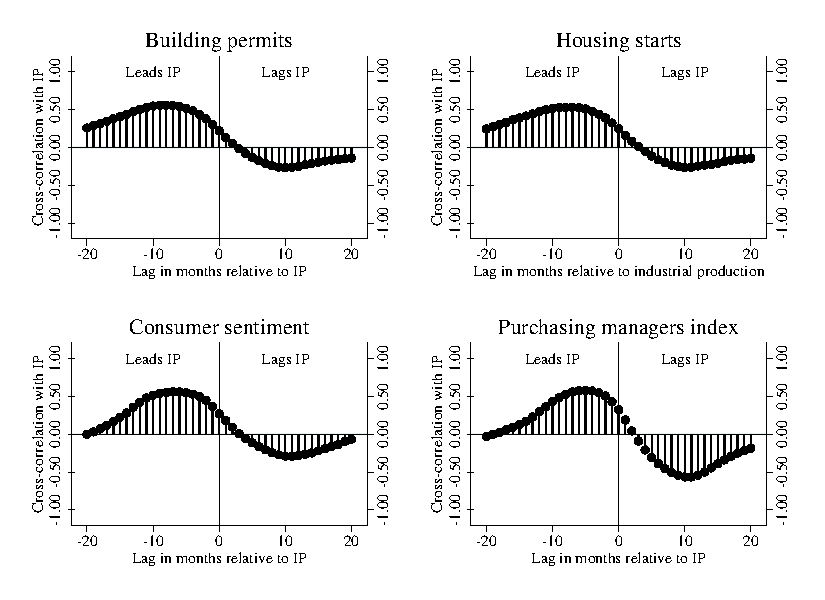
\includegraphics[width=0.8\textwidth]{\figpath Figures/xcsurvey.pdf}
\end{figure}

Other sources of useful information are various measures and surveys
of economic activity conducted by the Bureau of the Census and
private organizations.
Cross-correlation functions for four common ones are pictured in
Figure \ref{fig:ccf-survey}.
The first two are \href{http://research.stlouisfed.org/fred2/series/PERMIT}{building permits} and \href{http://research.stlouisfed.org/fred2/series/HOUST}{housing starts},
two indicators of new home construction reported by the Census.
Two ideas lie behind their use:
that construction of new capital is more volatile than other sectors
of the economy
and that decisions to build new homes reflect optimism about the future.
The cross-correlation functions suggest that they work;
while the correlations are
smaller than with (say) employment, the leads are substantial
(ten months or so).
The next two are popular private surveys.
\href{http://research.stlouisfed.org/fred2/series/UMCSENT}{Consumer sentiment},
based on a survey of consumers
collected by the University of Michigan, reflects consumers' optimism about current and future economic conditions.
The \href{http://research.stlouisfed.org/fred2/series/NAPM}{purchasing managers index} is what we call a ``diffusion index.''
It's based on a survey of purchasing managers who report whether
they see economic activity increasing or decreasing.
Each is used as is.
We see in the figure that both are procyclical \index{business cycle!procyclical}
 leading indicators.

We could go on.  There are hundreds of indicators, more all the time.
The most common one we've skipped is the slope of the yield \index{bond!bond yield}
 curve:
Flat or downward-sloping yield \index{bond!bond yield}
 curves are associated with slower-than-usual
future growth in output. More on this in the Appendix.\index{cross-correlation function|)}


\section{The business-cycle scorecard \index{business cycle!scorecard}}

Now that we understand how to identify good indicators,
how do we put them to work?
The central question here is how to combine the inputs of multiple indicators.
One way to do that is to summarize them informally, which is what we do here.
Another is to use multivariate regression, which is the next topic,
but not one we'll spend much time on in this course.

The business-cycle scorecard \index{business cycle!scorecard}
 is a summary of
what selected indicators tell us about near-term economic conditions.
We'll use the four monthly indicators pictured
in Figures \ref{fig:ip_emp} and \ref{fig:newclaims_hs}.
In the first figure, we see the monthly growth rate
of IP (top panel) and the change in (nonfarm) employment
for the period 1960 to the present.
They show similar patterns, with the major postwar
downturns evident in each.
Evidently, employment is procyclical\index{business cycle!procyclical},  rising in good times
and falling in bad times.
Industrial production is a ``noisier'' series, which is one reason that
many analysts prefer employment as a measure of current economic
conditions. The lines show us the mean value (the solid line)
and plus and minus
one standard deviation (the dashed lines).
The lines are useful benchmarks for telling how strong the
current value of an indicator is relative to past experience.

\begin{figure}[!ht]
     \caption{Industrial production and employment.}
    \label{fig:ip_emp}%
    \centering
    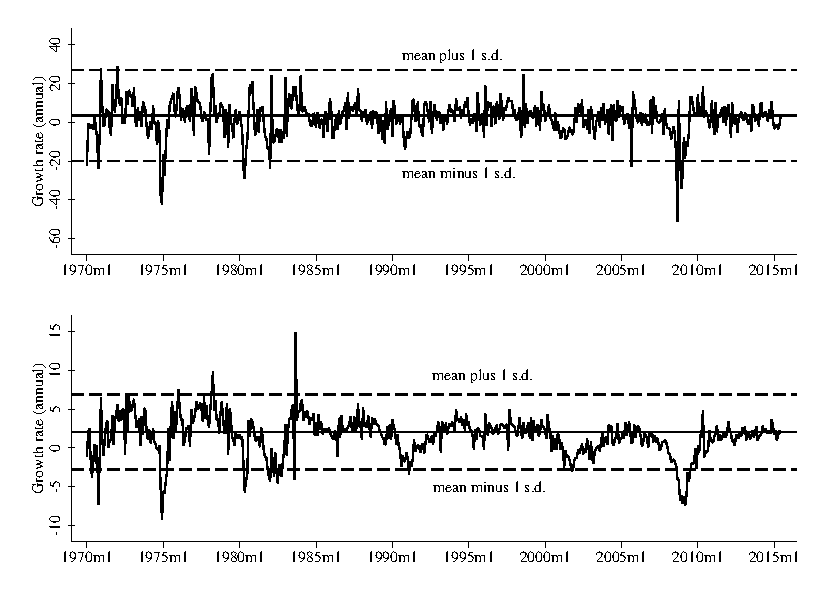
\includegraphics[width=0.9\textwidth]{\figpath Figures/scorecard_1.pdf}
    \begin{minipage}{0.85\textwidth}
    {\footnotesize The two panels show, respectively,
    the annual growth rate of industrial production and
    the year-over-year change in the number of people employed.}
    \end{minipage}
\end{figure}

\begin{figure}[!ht]
    \caption{New claims and housing starts.}
    \label{fig:newclaims_hs}%
    \centering
    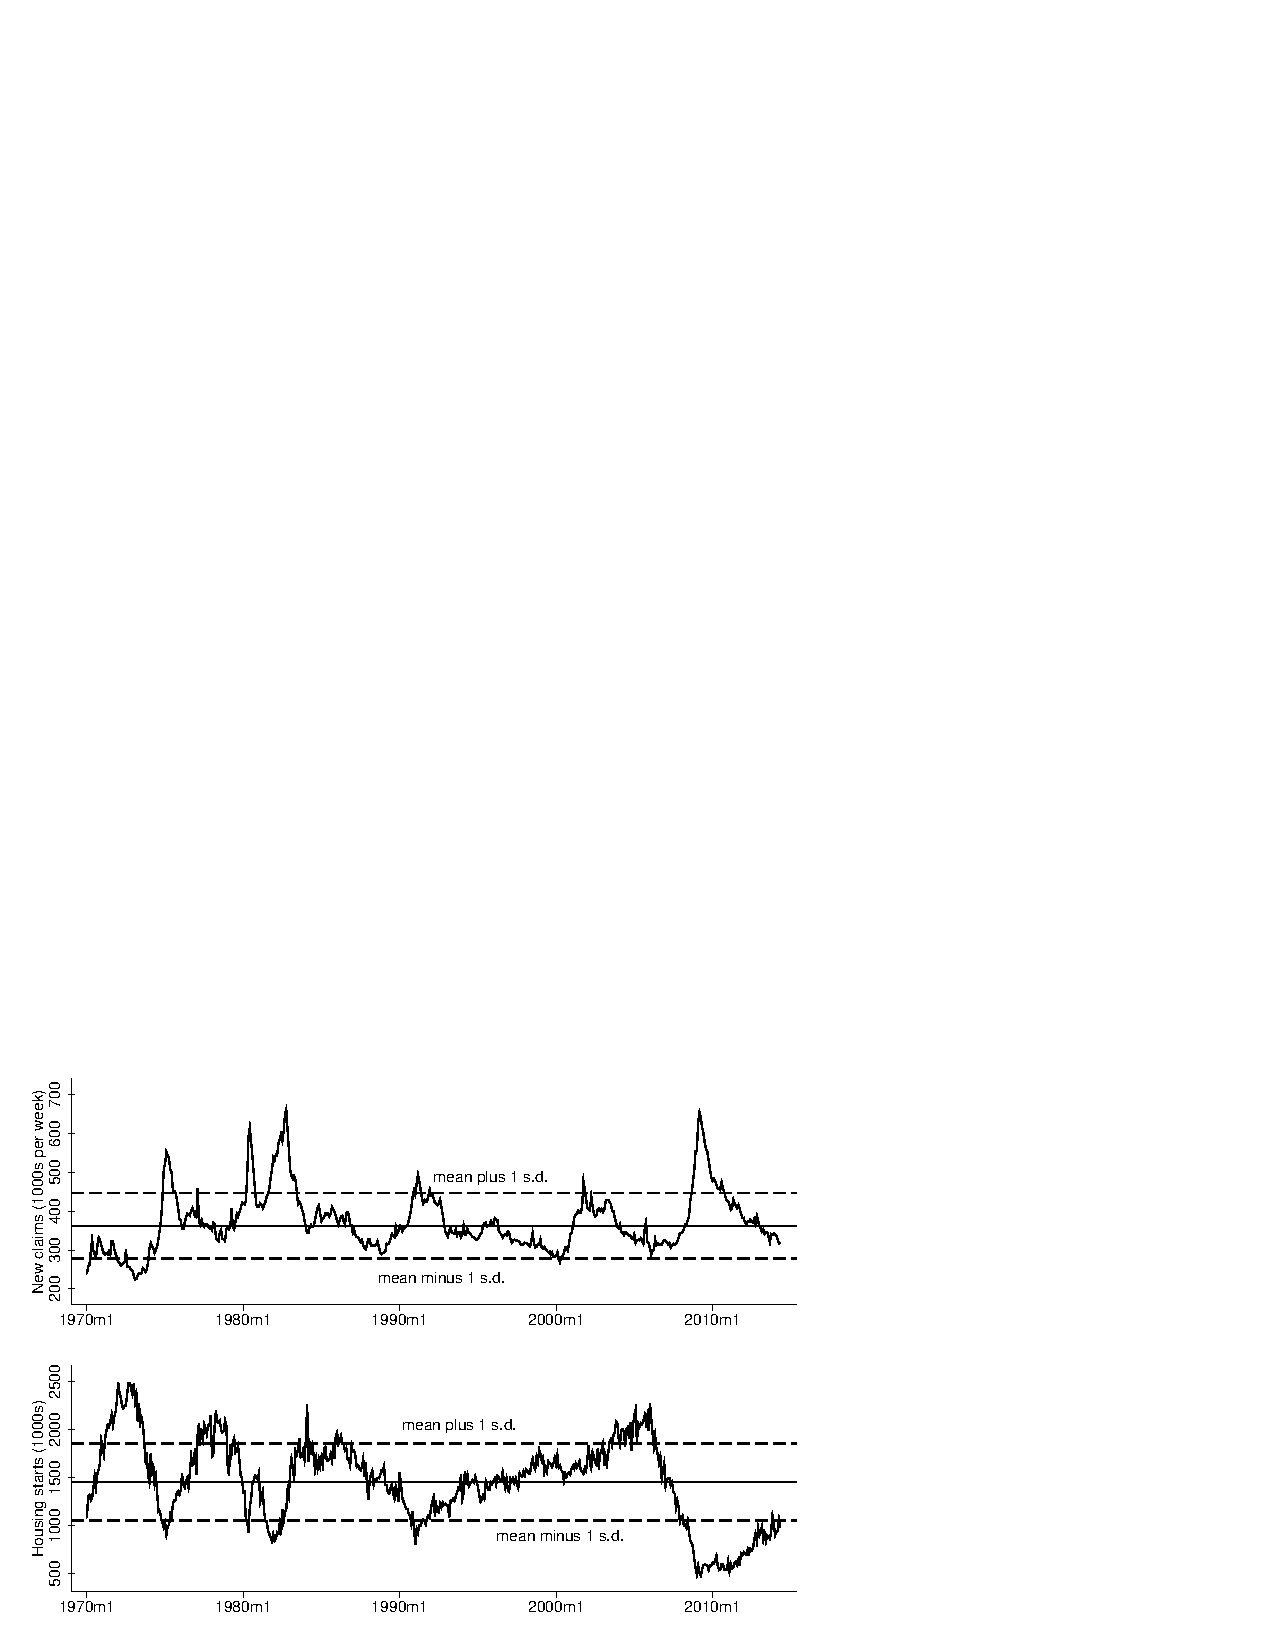
\includegraphics[width=0.9\textwidth]{\figpath Figures/scorecard_2.pdf}
    \begin{minipage}{0.85\textwidth}
    {\footnotesize The two panels show, respectively,
    new claims for unemployment insurance
    and housing starts, two popular indicators of economic conditions.}
    \end{minipage}
\end{figure}


In the second figure (Figure \ref{fig:newclaims_hs}),
we see similar data for new claims for unemployment insurance
and housing starts.
New claims are reported weekly; the figure is
based on the four-week moving average.
Remember, they are countercyclical:  they rise when the economy weakens.
The second panel is housing starts.
You can see in the figure that housing starts don't always go up
and down with the economy.
In the 2001 recession,
housing starts fell only slightly.
In 2008, we made up for that,
with housing starts falling to their lowest point
since (at least) 1960.
None of that will come as a surprise to you.
These four indicators come from the Federal Reserve (industrial production),
the Bureau of Labor Statistics (employment, new claims),
and the Bureau of the Census (housing starts).
These government agencies are the primary sources of economic indicators
in the US.
There are private indicators also,
but the government indicators are widely used and publicly available.

In the business-cycle scorecard\index{business cycle!scorecard},
we rate each pro-cyclical indicator \index{cyclical indicators}
 as strong positive if
the current value of the indicator is above the
``mean plus one standard deviation'' line,
weak positive if it's between the mean line and the one above it,
weak negative if it's below the mean line but above
the ``mean minus one standard deviation'' line,
and strong negative if it's below the bottom line.
For   countercyclical   \index{business cycle!countercyclical}
 indicators we reverse the direction:
for example, strong positive means below the ``mean minus one standard deviation'' line.

This is a rough cut, to be sure, but a useful one.
It leads to this summary of economic conditions as of August 2014
based on the four indicators we have seen so far:
\begin{itemize}
    \item Industrial production:
    Growth has been close to the mean over the last couple years.
    Assessment:  weak positive.

    \item Employment growth:  The most recent numbers show steady moderate growth.
    Assessment:  weak positive.

    \item New claims:  They are the only countercyclical indicator in our list. They have fallen dramatically over the last two years, and are now below the long-run average.
        Assessment:  weak positive.

    \item Housing starts:  They remain very low by historical standards, although there has been improvement since 2009. Assessment:  strong negative.
\end{itemize}


\begin{table}[!ht]
\centering
\caption{Business-cycle scorecard in action} %:  US economic conditions in January 2010.}
\begin{tabular}{lcccc}
\toprule
            &  Strong    &  Weak  &  Weak   &  Strong  \\
Indicator   &  Negative  & Negative & Positive & Positive \\
\midrule
Industrial production  & &  & x \\
Employment             & &  & x \\
New Claims             && &x \\
Housing starts         & x &  \\
\midrule
Summary                & 1 & 0 & 3 & 0 \\
\bottomrule
\end{tabular}
\label{tab:scorecard}
\end{table}

These assessments are collected in Table \ref{tab:scorecard}.
Overall, we see three weak positives and one strong negative,
a mixed set of signals that's not unusual.
A more extensive analysis would use more indicators,
decide how much weight to give each one,
assess how far into the future they point, and so on.


\section{Regression-based forecasting}

A more formal statistical approach is to include
as many indicators as we like in a multivariate regression.
We estimate the regression by some appropriate method
and use it to forecast the future.
Here are the steps we might follow in constructing a forecast
of (say) industrial production $k$ months in the future.

The first step is to construct the variable we're forecasting.
Let us say that we're interested in the growth rate of industrial
production between now and $k$ months in the future.
You can do what you want, but we compute the (annualized) growth
rate this way:
\[
    \gamma_{t,t+k} \;=\; \ln (\IP_{t+k}/\IP_t) \times (12/k) .
\]
We refer to $k$ (here measured in months) as the {\it forecast
horizon\/}.  The adjustment factor ``$12/k$'' converts the growth
rate to annual units.
For a one-year forecast, then, we would set $k=12$ and compute the
year-on-year growth rate.

The second step is to find some variables you think would be useful
in forecasting.
The previous section might give you some ideas.
There's a half-step that sneaks in about here, too:
what form of the indicator to use.
In most cases, we use growth rates of the indicators, too,
either over one period or a year,
whichever you think works best.
But some variables are used as is.
In Figure \ref{fig:ccf-labor}, for example,
the cross-correlation for the unemployment rate is for the rate, period --- not its growth rate, change, or other transformation.

Third, you put all the ingredients into a statistical package and run a regression.
For example, to forecast IP growth, we would estimate the regression
\[
        \gamma_{t,t+k}  \;=\;  a + b x_t + \mbox{residual},
\]
where $x_t$ is the value of the indicator we have chosen.
We use a sample of data to estimate the parameters $a$ and $b$.
Note well:  The growth rate is between now (date $t$)
and a future date ($t+k$),
but the indicator is observed now (at $t$).
This is central to the exercise:  We use what we know now
to predict the future.
It's not kosher to use future variables to predict the future
because we don't know the future when we make the forecast
(duh!).


Fourth and last:
Once we have estimates of the regression
parameters ($\widehat{a}$ and $\widehat{b}$, say),
we use them and the current value(s)
of the indicator(s) ($x$, say)
to compute the forecast:
\[
        \widehat{\gamma}_{t,t+k}  \;=\;  \widehat{a} + \widehat{b} \; x_t .
\]
The ``hats'' remind us that we are using estimates;
$\widehat{\gamma}_{t,t+k}$ is our forecast of future growth.
There are lots of variants of this approach --- you can add multiple indicators,
lags of the indicators  ($x_{t-1}, x_{t-2}, ...$),
and even past values of the growth rate of industrial
production.
We recommend all of the above.


The result of such an exercise is generally a useful forecast --- useful in the sense that it tells us something about the future.
Something, but not everything!
Over periods of a year or two, forecast accuracy is usually modest.
Even in-sample, the regressions rarely have $R^2$s above 0.25,
which tells us that most of the variation (at least 75 percent) in our forecast variable is unexplained.
Some people see a lesson in this:  It might be more important
to know how to respond when the unexpected occurs
than to have better forecasts.
In practice, both are useful:  knowing something about the future,
and having backup plans to deal with the inevitable forecasting errors. It pays to carry an umbrella when the forecast calls for rain.\index{industrial production|)}


\section{Aggregation and prediction markets}

There's another appealing approach to forecasting: Let markets do the work.
Most of the best forecasts aggregate information from multiple
indicators and sources.
Indexes of leading indicators do this one way by combining multiple indicators to produce an index, which is then used
to forecast the future.
Or we could use multiple indicators in regression-based forecasts,
as we suggested above.

Another approach is to aggregate the forecasts themselves --- that is take several forecasts, perhaps based on different indicators, and average them.
The business-cycle scorecard \index{business cycle!scorecard}
 is a simple version of this.
The so-called ``Blue Chip" forecast is an average of forecasts generated by experts, and it performs better than any single forecaster.
Some statistical forecasters do the same sort of thing on their own.
They generate multiple forecasts with methods like our forecasting regression, and then average them to generate a final aggregate forecast. Again,
the aggregate tends to do better than the individual forecasts.

A related idea is to rely on markets, which aggregate information
from the people using them.  \href{http://tippie.uiowa.edu/iem/markets/pres12.html}{Presidential futures markets}, for
example, have predicted the popular vote in the last four
elections more accurately than any of the major polls. \index{presidential futures markets}
In the economic arena, there are a growing number of markets
in which you can trade futures contracts whose payoffs are tied
to the value of specific economic numbers:
the consumer price index\index{price index!consumer price index (CPI)}, the fed funds rate, and so on.
These markets are increasingly used as forecasts themselves, with one wrinkle.
The simplest interpretation is that the futures price is a market forecast
of the relevant economic number.
For example, if we are interested in the value of an economic number $y$
to be released in 6 months ($y_{t+6}$, say),
we might use its current futures price ($f_t$, say):
\[
    f_t  \;=\;  \mbox{Market's Current Forecast of } y_{t+6} .
\]
Experience (and possibly some insight) tells us that we may want to make a
correction for the risk of the contract:
\[
    f_t  \;=\;  \mbox{Market's Current Forecast of } y_{t+6}
                + \mbox{Risk Premium} .
\]
There's no limit to the amount of sophistication
we can bring to bear on the last term,
but for now, you can simply note that
we probably want to address it in some way.
Once you do, markets are an extremely useful source of information
about the future.
%An application to the yield \index{bond!bond yield}
%curve is included in the Appendix at the end of this chapter.


\section*{Executive summary}

%\setlength{\leftmargini}{.5\oldleftmargini}
\begin{enumerate}
\item Fluctuations in economic activity can be (partially)
predicted by a number of indicators.

\item The cross-correlation function is a tool for describing the
timing of the relation between two indicators:
for example, whether one indicator leads another.

\item Markets are useful aggregators of information --- and increasingly popular sources of economic forecasts.
\end{enumerate}
%\setlength{\leftmargini}{\oldleftmargini}


\section*{Review questions}

%\setlength{\leftmargini}{.5\oldleftmargini}
\begin{enumerate}
\item Terminology. Consider economic indicators in general.
\begin{enumerate}
\item What is a procyclical indicator? A   countercyclical
 indicator?
\item Give an example of each.
\item What is a leading indicator?  A lagging indicator?
\item Give an example of each.
\end{enumerate}

Answer.
\begin{enumerate}
\item A procyclical indicator moves up and down with GDP.
A   countercyclical
 indicators goes up when GDP moves down.
We typically identify this feature with the sign of the correlation.
\item Most indicators are procyclical
:  employment, the S\&P 500, and so on.
The unemployment rate is the classic   countercyclical
 indicator.
\item A leading indicator is correlated with future GDP growth,
a lagging indicator is correlated with past GDP growth.
\item The stock market is a leading indicator,
the unemployment is a lagging indicator.
We typically identify this feature with the cross-correlation function.
\end{enumerate}


\item Housing starts.
We mentioned housing starts as an indicator
of future economic activity.
In what ways do you think it's a good indicator?  A bad one?
(For further information, see the US Census Bureau's
\href{http://www.census.gov/construction/nrc/}
{web site}.)

Answer.  Good:  connected to housing, which, as a durable good,
should be cyclically sensitive and volatile; available quickly; it
leads the cycle (as you can see from its ccf). Bad: based on a sample,
which leads to short-term noise; revised periodically;
strong seasonality;
possibly misleading now that we have a glut of housing to work off.

\item Unemployment.  The unemployment rate is widely reported in the press,
but professionals rarely use it.  Why do you think that is?

Answer.
One reason is that the unemployment rate understates the
change in employment in a downturn.
Some people who lose jobs leave the labor force,
so they're not included in the unemployment rate.
Another reason is that the unemployment rate is a lagging
indicator.
It falls slowly, well after the economy turns around.
Employment (the number of people actually working) is
the preferred indicator for both reasons.

%\item The term spread (a long yield \index{bond!bond yield}
% minus a short yield
%is positively correlated with future output growth.  Why do you think that is?
%
%Answer. A steep yield \index{bond!bond yield}
% curve means that we expect
%short-term interest rates to rise.  Short-term interest rates may
%rise because the economy is growing quickly (interest rates are
%typically higher in booms) and/or because we expect higher
%inflation (sometimes associated with a booming economy).

\item Terrorism futures.
In 2002, a government agency recommended that we establish a
futures market in terrorist attacks, on the grounds that it would
give us a useful public indicator of their likelihood.  The idea
was widely criticized.  Do you think it was a good idea or a bad
one?  What would you need to do to implement it?

Answer.  Another case of a good idea thrown out because it sounded
bad to politicians.  It's not clear that such attacks are predictable,
but if they are, we'd expect futures markets to do as well as any
other method.  To implement the idea, you'd need to define (and
possibly quantify) a terrorist event.
\end{enumerate}
%\setlength{\leftmargini}{\oldleftmargini}


\section*{If you're looking for more}

There are many sources of leading indicators around the world
and almost as many guides to them.
Among them:
%
\begin{itemize}

\item The best book we've seen on the subject is
Bernard Baumohl,
\href{http://www.amazon.com/The-Secrets-Economic-Indicators-Opportunities/dp/0132932075/}
{\it The Secrets of Economic Indicators\/}.
If you use economic indicators in your job, you should buy this book.

\item The Bloomberg
\href{http://www.bloomberg.com/markets/ecalendar/index.html}
{Economic Calendar}
gives release dates and short summaries of a wide range of indicators.
Ditto the WSJ, Yahoo, etc.

%\item The Conference Board,
%\href{http://www.conference-board.org/pdf_free/economics/bci/BCI-Handbook.pdf}
%{\it Business Cycle Indicators Handbook\/}.

\item The CME has a nice report,
``\href{http://www.cmegroup.com/education/featured-reports/impact-of-economic-indicators.html}
{Impact of economic indicators},''
on the information content of common indicators for futures prices.
%\href{http://www.cmegroup.com/trading/economic-events/files/Economic-Indicators-WhitePaper.pdf}


%\item Jim Stock and Mark Watson are the two leading academics working on
%economic indicators.  Their 2003 paper in the Richmond Fed's {\it Economic Review\/}
%is an interesting look back at the 2001 recession
%and why many didn't see it coming.
%Here's a
%\href{http://www.richmondfed.org/publications/economic_research/economic_quarterly/pdfs/summer2003/stockwatsonsummer03.pdf}.
%{link}.
%\item The National Bureau of Economic Research
%runs an email alert service
%for major macroeconomic data releases, primarily for the US.
%%See \href{http://nber.org/releases/}{link}.
\end{itemize}
%
Most statistical software packages have one-line commands to compute
cross-correlation functions.
You can also do it in a spreadsheet, but it's a lot more cumbersome.

To do more with this topic, you need some knowledge of time series statistics.
If you'd like to learn more about forecasting economic and
financial variables specifically,
we recommend ``Forecasting Times Series Data,'' course STAT-GB.2302,
taught in alternate years by Professors Deo and Hurvich, two of our best statisticians.

\section*{Symbols and data used in this chapter}

\begin{table}[H]
\centering
\caption{Symbol table.}
\begin{tabular*}{1.0\textwidth}{l@{\extracolsep{\fill}}l}
\toprule
Symbol & Definition\\
\midrule
$\mathrm{ccf}$             &Cross-correlation function \\
$\mathrm{ccf}(k)$         &Correlation of ($x_t, y_{t-k}$) at lag $k$\\
$\gamma_{t,t+k}$         &Continuously compounded growth rate from $t$ to $t+k$\\
$\widehat{x}$                & Estimate of $x$\\
$f_t$                     & Futures price at time $t$\\
%$p_m$                     &Price of an $m$-year zero-coupon bond \index{bond}\\
%$y_m$                     &yield \index{bond!bond yield}
% of an $m$-year zero-coupon bond \\
%$f_n$                     &One-period forward interest rate n-periods ahead\\
%$f_{n,t}$                 &One-period forward rate arranged at time $t$ for $n$ periods ahead\\
%$i_t$                     &One-period interest rate that prevails in period $t$\\
%${E}_t(x)$         &Expected value at time $t$ of $x$\\
\bottomrule
\end{tabular*}
\end{table}

\begin{table}[H]
\centering
\caption{Data table.}
\begin{tabular*}{0.75\textwidth}{l@{\extracolsep{\fill}}l}
\toprule
Variable & Source\\
\midrule
Industrial production        &INDPRO\\
Real GDP                    &GDPC1\\
S\&P 500                        &SP500\\
Employment                    &PAYEMS\\
Unemployment rate            &UNRATE\\
New claims                    &IC4WSA\\
Hours worked                &AWHMAN\\
Building permits            &PERMIT\\
Housing starts                &HOUST\\
consumer sentiment             &UMCSENT\\
Purchasing managers' index    &NAPM\\
10-year Treasury yield
            &GS10\\
2-year Treasury yield
            &GS2\\
Federal funds rate            &FEDFUNDS\\
\bottomrule
\addlinespace
\end{tabular*}
\begin{minipage}{0.75\textwidth}
\footnotesize{To retrieve the data online, add the identifier from the source column to \url{http://research.stlouisfed.org/fred2/series/}.  For example, to retrieve nonfarm employment, point your browser to \url{http://research.stlouisfed.org/fred2/series/PAYEMS}}
\end{minipage}
\end{table}


\begin{comment}
\newpage
\section*{Appendix:  Reading the yield \index{bond!bond yield}
 curve }
\phantomsection
\label{sec:yield_curve}

\subsection*{The yield \index{bond!bond yield}
 curve}

We use the yield \index{bond!bond yield}
 curve to infer ``the
market's'' forecast of future short-term interest rates.
Roughly speaking, the slope of
the yield \index{bond!bond yield}
 curve tells us what the market expects of future
short-term interest rates. But before we explain how this works,
we need to review yields \index{bond!bond yield}
 and forward rates. \index{interest rate!short-term}
Most of this should be familiar if you've taken
``Foundations of Finance.''

yields \index{bond!bond yield}
 and forward rates are subspecies of interest rates. {\it
yields \index{bond!bond yield}
\/} are simply a way of reporting bond \index{bond} prices. If you go
into the bond \index{bond} business, you'll find there are lots of details to
worry about (accrued interest, day count conventions, etc.), but
we'll keep it simple and look at yields \index{bond!bond yield}
 on bonds \index{bond} with no coupons --- zero-coupon bonds \index{bond} or ``zeros.''
 A one-year zero is a claim to (say) \$100 in
one year.  A two-year zero is a claim to \$100 in two years.  An
$m$-year zero is a claim to \$100 in $m$ years, and so on.  If the
price of an $m$-year bond \index{bond} is $p_m$, its yield \index{bond!bond yield}
 $y_m$ is defined by
the present-value formula:
\begin{equation}
        p_m  \;=\; 100/(1+y_m)^m.
        \label{eq:pv}
\end{equation}
This formula is based on annual compounding \index{annual compounding}
, which is the most
convenient convention for our purposes; more on this shortly. Note
that if we know prices, we can find yields \index{bond!bond yield}, and vice versa. The
{\it yield \index{bond!bond yield}
 curve\/} for zero-coupon bonds \index{bond} is a graph of yield \index{bond!bond yield}
$y_m$ versus maturity $m$.


The yield \index{bond!bond yield}
 curves you see in the newspaper are usually based on
yields \index{bond!bond yield}
 of coupon bonds \index{bond}, and in the case of US treasuries, they use
semi-annual compounding \index{annual compounding}
. They capture similar information, but
they're a little harder to make sense of.  Why?  Because the yield \index{bond!bond yield}

depends not only on maturity, but also on the coupon. Since
the coupons vary over time and across maturities, it's never
exactly clear what we're talking about.  For that reason, most
formal fixed-income analysis starts with prices and yields \index{bond!bond yield}
 of
zeros.


\textbf{Example.} Prices of zero-coupon bonds \index{bond} are given in Table \ref{tab:bond}. What are the yields \index{bond!bond yield}
?
%
\begin{table}[H]
\centering
\caption{Example bond \index{bond} prices.}
\begin{tabular}{cc}
\toprule
               Maturity        &     Price         \\
\midrule
                1              &      94.24        \\
                2              &      87.70        \\
                3              &      81.22        \\
                4              &      75.16        \\
                5              &      69.66\\
\bottomrule
\end{tabular}
\label{tab:bond}
\end{table}
%

Answer.  The yields
 are 6.11, 6.78, 7.18, 7.40, and 7.50,
respectively, expressed as annual percentages.  The third one
solves the equation $ 81.22 = 100/(1+y_3)^3 $, namely $ 1 + y_3 =
(100/81.22)^{1/3} $.  The others are similar.


Yields \index{bond!bond yield}
 are interest rates that apply over a number of periods. For
example, the $m$-year yield \index{bond!bond yield}
 at date $t$ applies over the period of
time between $t$ (now) to $t+m$ ($m$ years from now).  One way to
think about the return on the bond \index{bond} is that the holder invests $p$ and
gets a rate of return equal to the yield \index{bond!bond yield}
 $y$ for every period
until maturity.  In the two-period case, this leads to
\[
    100 \;=\; p_2 \times (1+y_2) (1+y_2) ,
\]
a variant of our present-value formula, equation (\ref{eq:pv}).
Another way to think about the return is that the rates vary
across periods. In the two-period case, the bond \index{bond} might have
different rates of return in the first and second periods. But
what are these returns?  We know that the return on a one-period bond \index{bond}
is $y_1$, so the first-period return should be $y_1$.  What about
the second period?  We need an interest rate that applies to the
second period alone but that remains consistent with the price of
the bond. \index{bond} That is, a rate $f_1$ that satisfies
\[
    100 \;=\; p_2 \times (1+y_1) (1+f_1) .
\]
Putting these two equations together tells us
\[
    (1+y_2)^2 \;=\; (1+y_1) (1+f_1)
\]
or
\[
    1+f_1 \;=\; p_1/p_2 .
\]
We refer to $f_1$ as the one-period-ahead {\it forward rate\/},
since it applies at date $t$ to the time period between $t+1$ and
$t+2$. It's the rate of return on a {\it forward contract\/} in
which we agree at $t$ to invest a fixed amount at $t+1$ for one
period.
For our purposes, you can think of forward contracts
as identical to the more common futures.
The latter differ (a little) in having a mark-to-market requirement,
which aficionados will take seriously, but the rest of us can safely
ignore.

The same logic applies to bonds \index{bond} with maturities greater than two.
The bond \index{bond} price can be expressed as
\begin{eqnarray*}
        p_m &=& 100/(1+y_m)^m \\
            &=& 100/ [(1+y_1)(1+f_1) \cdots (1+f_{m-1})] .
\end{eqnarray*}
The two relations together imply
\begin{equation}
    1+f_{m-1} \;=\; p_{m-1}/p_{m} ,
    \label{eq:fdef}
\end{equation}
where $f_m$ is the $m$-period-ahead forward rate.  Draw a circle
around this equation since you'll be using it soon.  What we're doing
here is using bonds \index{bond} of two consecutive maturities to ``pick off''
the forward rate that applies over the last period.

Putting all the pieces together, we have three ways to express the
same information:  bond \index{bond} prices, yields \index{bond!bond yield}
, and forward rates. Given
data on a complete set of maturities, we can compute any one of
the three from any other.

\textbf{Example (continued).} For the bond \index{bond} prices and yields \index{bond!bond yield}

reported earlier, verify that the forward rates are the ones reported in Table \ref{tab:forwards}.
%
\begin{table}[H]
\centering
\caption{Example forward rates.}
\begin{tabular}{cccc}
\toprule
  Maturity ($m$)  &  Price ($p_m$)  &  yield
 ($y_m$)  & Forward Rate ($f_{m-1}$) \\
  \midrule
     1      &  94.24  &   6.11 &   6.11    \\
     2      &  87.70  &   6.78 &   7.45         \\
     3      &  81.22  &   7.18 &   7.98     \\
     4      &  75.16  &   7.40 &   8.06       \\
     5      &  69.66  &   7.50 &   7.90\\
     \bottomrule
\end{tabular}
\label{tab:forwards}
\end{table}
Note that the maturities of forward rates are one less than those
of bond \index{bond} prices and yields \index{bond!bond yield}
.  We do this because they naturally
start at zero, for reasons that may be clearer to you shortly. The
0-period-ahead forward rate is simply the current one-period
yield \index{bond!bond yield}
:   $f_0 = y_1$.

Answer.  We compute forward rates from prices.  For $m=5$, the
calculation implied by equation (\ref{eq:fdef}) is
\[
    1 + 0.0790 \;=\; 75.16/69.66.
\]
The others are similar.


\subsection*{Reading the yield \index{bond!bond yield}
 curve}

Now that we've done all this work, we can use it to predict future
one-period yields \index{bond!bond yield}
.  Put simply but somewhat imprecisely, we're
going to say that forward rates are the market's expectation of
future one-period yields \index{bond!bond yield}
, plus an adjustment for risk that depends
on maturity but doesn't vary over time.  Once we've done the
adjustment, we can read expected future one-period yields \index{bond!bond yield}
 from the
forward rate curve. The idea is referred to as the {\it
expectations hypothesis\/} because it's based on the premise that
forward rates include expectations of future one-period yields \index{bond!bond yield}
 --- {\it short rates\/} in conventional terminology.

To be more precise, we need to add a little notation. Since we'll be dealing a lot with the
one-period yield \index{bond!bond yield}
 or short rate, let us label it $i$, so that $i_t$ is the yield \index{bond!bond yield}
 on a one-period
bond \index{bond} bought at date $t$. We label (one-period) forward rates by $f_{m,t}$, meaning the rate on a
forward contract arranged at date $t$ but applying to the period between dates $t+m$ and $t+m+1$.
The expectations hypothesis states that the forward rate is the market's expectation or forecast
of the future short rate plus a risk premium:
\begin{equation}
    f_{m,t} \;=\; E_t (i_{t+m}) + \mbox{risk premium}_m .
    \label{eq:eh}
\end{equation}
The risk premium is assumed to be constant across time but may
vary by maturity.  The notation $E_t$ is meant to convey the
expectation made at date $t$.  If we know forward rates and risk
premiums, we can compute expected future short rates.


That's what the expectations hypothesis is, but where does it come
from?  Let's think about what an investor would demand of a
forward rate.  An investor with a two-period time horizon has (at
least) two choices.  She could buy and hold a two-period bond \index{bond} at
date $t$, thus getting (according to our second interpretation)
returns of $ i_t $ in the first period and $ f_{1,t} $ in the
second.  Alternatively, she could roll over a one-period bond \index{bond},
getting (again) $i_t$ in the first period and the short rate $
i_{t+1} $ in the second.  These two possibilities can be pictured this way:
%
\begin{center}
\unitlength=0.6mm
\begin{picture}(100,50)
  \put(50,45){\makebox(0,0){Rollover Strategy}}
  \put(25,32){\makebox(0,0){$i_t$}}
  \put(75,32){\makebox(0,0){$i_{t+1}$}}
  \put(0,25){\line(100,0){100}}
  \put(0,25){\makebox(0,0){$  |  $}}
  \put(50,25){\makebox(0,0){$  |  $}}
  \put(100,25){\makebox(0,0){$  |  $}}
  \put(25,18){\makebox(0,0){$i_t$}}
  \put(75,18){\makebox(0,0){$f_{1,t}$}}
  \put(50,5){\makebox(0,0){Buy and Hold Strategy}}
\end{picture}
\end{center}
%
If $ i_{t+1} $ were known, then we would expect the market to
drive the forward rate $ f_{1,t} $ and the future short rate $
i_{t+1} $ together:  $ f_{1,t} = i_{t+1} $. If the future short
rate were higher, then no one would buy the long bond. \index{bond}  Its price
would fall and the forward rate would rise.  If it were lower,
everyone would buy the long bond \index{bond} and bid up its price. In an
uncertain world, similar logic might lead us to guess that the
forward rate is the market's forecast of the future short rate,
with some adjustment for risk:
\[
    f_{1,t}   =  E_t ( i_{t+1} ) + \mbox{\em risk premium}   .
\]
Similar reasoning for longer maturities leads us to equation
(\ref{eq:eh}).


The only remaining issue is estimating the risk premiums.  There
are as many ways to do this as there are finance professors, but a
relatively simple method is to use the average difference between
the short rate and the $n$-period forward rate as an estimate of
its risk premium; that is, we use
\begin{equation}
    \mbox{risk premium}_m  \;=\; E (f_{m,t}  -  i_{t} )
\end{equation}
and estimate the expectation on the right with the mean. This
should work as long as forecast errors (the difference between the
future short rate and its expectation) are zero, on average, and
the distribution of the short rate doesn't change over time (the
means of the short rate and future short rate are the same).
Table~\ref{tab:meanrates} summarizes mean forward rates for US
treasuries for the period 1970-2000.  Since the short rate is the
first forward rate, we compute risk premiums by subtracting it
from the other forward rates.

\begin{table}[H]
\centering
\caption{Mean forward rates for US Treasuries, 1970-2000.}
\begin{tabular}{ccc}
\toprule
        Maturity   &    Mean Forward Rate   &  Risk Premium \\
\midrule
            1  &  7.51 &  0.00 \\
            2  &  8.10 &  0.59 \\
            3  &  8.39 &  0.88 \\
            4  &  8.57 &  1.06 \\
            5  &  8.67 &  1.16  \\
\bottomrule
\end{tabular}
\label{tab:meanrates}
\end{table}

\textbf{Example (continued).} For the forward rates reported
earlier, what are the implied expected future short rates?

Answer.  The calculations are summarized by:
%
\begin{table}[H]
\centering
\caption{Example expected future short rates.}
\begin{tabular*}{0.9\textwidth}{c@{\extracolsep{\fill}}ccc}
\toprule
  Maturity & Forward Rate & Risk & Future Short Rate \\
    ($m$) &  ($f_{m-1}$) & Premium &  ($i_{t+m-1}$) \\
\midrule
     1      &   6.11       &    0.00      &    6.11 \\
     2      &   7.45       &    0.59      &    6.86  \\
     3      &   7.98       &    0.88      &    7.10  \\
     4      &   8.06       &    1.06      &    7.00  \\
     5      &   7.90       &    1.16      &    6.74\\
\bottomrule
\end{tabular*}
\end{table}

In short, we can read expected future short-term interest rates
from the forward rate curve, which we compute from the yield curve
for zeros.  If you find this interesting, there's a lot more on
related topics in the ``Debt Instruments'' course.
\end{comment}

\chapter{Money and Inflation}\label{chp:mpin}
\hypertarget{inflation}{}

%No extra line here.
\textbf{Tools:} The quantity theory; central bank balance sheet; open market operations.

\textbf{Key Words:} Price level; inflation; hyperinflation; quantity theory; velocity; fiscal dominance.

\textbf{Big Ideas:}
%\vspace{-0.1in}
\begin{itemize}
    \item Inflation is the growth rate of the price level, which is typically measured by a price index.
    \item The quantity theory links the money supply with the price level and output. In the long run, an increase in the money supply results in an increase in the price level (inflation).
    \item Hyperinflation refers to an inflation rate of 100\% per year or more.
    Hyperinflations follow a standard pattern: government deficits are financed with money, which produces inflation.
        We call this {\it fiscal dominance\/} over monetary policy.
\end{itemize}

\rule{\textwidth}{1pt}

Inflation\index{inflation} is the rate of growth of the price level,
typically measured by a price index. \index{price index}
If prices are rising, on average, we have inflation.
Milton Friedman, winner of the 1976 Nobel Prize in economics, once
said: ``Inflation is always and everywhere a monetary phenomenon.
To control inflation, you need to control the money supply.''
Friedman believed what he said, but he also enjoyed
thumbing his nose at the popular Keynesian theory of the 1960s,
in which inflation was the result of excess demand for goods.

Was Friedman right?
We consider his claim in the context of {\it hyperinflations\/}:\index{inflation!hyperinflation}
episodes of annual inflation exceeding 100 percent per year.
Although extreme, big inflations are a recurring phenomenon
and a wonderful laboratory for
studying inflation more generally.
In these situations (but not necessarily in others),
money growth is present,
but it's invariably connected to government deficits.
The keys to stopping a big inflation, then, are to
balance the government's budget and prevent the central bank from expanding the money supply.
The idea that inflationary monetary policy might stem from
fiscal policy is generally referred to as {\it fiscal dominance\/}.
\index{fiscal dominance}\index{government budget!budget deficit@budget (or government) deficit}


\section{The quantity theory \index{quantity theory of money}}

Friedman's claim about inflation\index{inflation} is based on a theory that is
several centuries old: the {\it quantity theory of
money\/}. \index{Friedman, Milton} Like a lot of good theory, it's based on an analogy. Think
for a moment about the effect of a two-for-one stock split on the
price of a stock. If it's now selling for 100, then you'd probably
expect it to sell for 50 after the split. (This wouldn't be true if
the split were a signal of some new information about the firm,
but let's assume it's not.) The point is that the value of a firm's
total stock of equity shouldn't depend on anything as arbitrary as
the number of shares.\index{quantity theory of money|(}

Now suppose we do the same thing with money.  This is
unrealistically simple, but makes the point effectively. Suppose that the
government replaced every dollar with two ``new dollars,''
marked so we could tell the difference between old and new notes. Then
you'd expect that new dollars would be worth half as much
as old dollars. That is, you'd expect prices of goods and services
quoted in new dollars to be twice as high as prices quoted in old
dollars. In short, changes in the quantity of money in circulation
(the ``money supply'') executed in this way will be associated with
proportionate changes in prices, with no effect on output.  Why the
latter? Because output is determined by productivity and inputs, and
we wouldn't expect either one to be influenced by the number of
pieces of paper used to make transactions.

Of course the world is more complicated than this, and monetary policy \index{monetary policy}
 consists of more than just currency exchanges, but some of
the same reasoning applies more generally (we'll look at some data
shortly). The quantity theory is the result of two ideas:  that
money is not fundamental (pieces of paper don't change the
productivity of the US or Chinese economies), and that its
usefulness is in executing transactions.  Let's start with the
latter. In all developed economies, transactions consist of
exchanges of goods and services for money. If we approximate the volume of
transactions in an economy by nominal GDP, then we have
$M=PY$, where $Y$ is real GDP\index{gross domestic product (GDP)!real GDP} and $P$ is a measure of the
price level such as the GDP deflator.  This isn't quite right yet. A
dollar can be used to execute several different transactions in a
given year.
To take this into account, we use
%
\begin{eqnarray}
    M V  &=&  P Y,
%    M_t V_t  &\equiv&  P_t Y_t,
    \label{eq:quantity_theory}
\end{eqnarray}
%
where $V$ is the \textit{velocity} of money: the number of times a
dollar is used to execute transactions in a given year.

At this level of generality,
equation (\ref{eq:quantity_theory}) is a tautology:
For any data we collect on $M$, $P$, and $Y$,
we simply choose $V$ to make the equation hold.
What gives the equation content is Friedman's
assumption that velocity \index{velocity of money}
 $V$ is (at least approximately)
constant.  This implies that increases in $M$ are associated with
proportionate increases in $PY$.
We add one further assumption to get Friedman's connection between
money and prices:
that real GDP\index{gross domestic product (GDP)!real GDP} is determined by the productivity and inputs of the economy,
and is not affected by the amount of money in circulation.
We can --- and will --- change that later, but it seems like a good place to start.


The same theory explains inflation\index{inflation} if we express it in growth rates.
As with growth accounting, we focus on \hyperref[sec:growth_math_cc]{continuously compounded growth rates} where the growth rate of a variable $X$ is
$ \gamma_X = \ln X_t - \ln X_{t-1}$.
In logs, equation (\ref{eq:quantity_theory}) and its first difference are:
%
\begin{eqnarray*}
    \ln M_t + \ln V_t &=& \ln P_t + \ln Y_t \\
    (\ln M_t - \ln M_{t-1})  + (\ln V_t - \ln V_{t-1})
                 &=& (\ln P_t - \ln P_{t-1}) + (\ln Y_t - \ln Y_{t-1})\\
    \gamma_M  + \gamma_V &=&  \pi + \gamma_Y ,
\end{eqnarray*}
%
where $\pi = \gamma_P $ is the inflation rate
(the rate of growth of the price level).
If we assume that velocity is constant,
\begin{eqnarray}
    \gamma_M   &=&  \pi + \gamma_Y ,
    \label{eq:quantity_theory-growth}
\end{eqnarray}
and changes in the growth rate of money are associated
with changes in the growth rate of inflation\index{inflation} and output.
The second assumption is that the growth rate of money does not influence
output, so changes in money growth translate one-for-one
into changes in inflation.
That's Friedman's argument, which depends on these two assumptions.


\section{Evidence}

It's not that easy to check the second assumption, but we can
check the first (constant velocity) by looking at the components of
equation (\ref{eq:quantity_theory}).
If velocity is constant, movements in the price
level $P$ mirror those in $M/Y$.
We check this in Figure~\ref{fig:quantity_long}, which graphs
both variables for the US.
(Money here is \href{http://research.stlouisfed.org/fred2/series/M2}{M2}.)
The figure suggests that the theory is a reasonable approximation of the data, at least
over the last fifty years or so.
The two increasing lines ($P$ and $M/Y$)
show some differences, but their long-run movements are similar.
Overall, velocity has been largely flat,
but since the financial crisis of 2007-09 it has
fallen amid record low interest rates.
Time will tell whether or not the change is temporary.
%Velocity itself wiggles around a little, but is not
%much different now than it was in 1960.
%
\begin{figure}[ht]
    \caption{The quantity theory in the long run.}
    \label{fig:quantity_long}
    \centering
    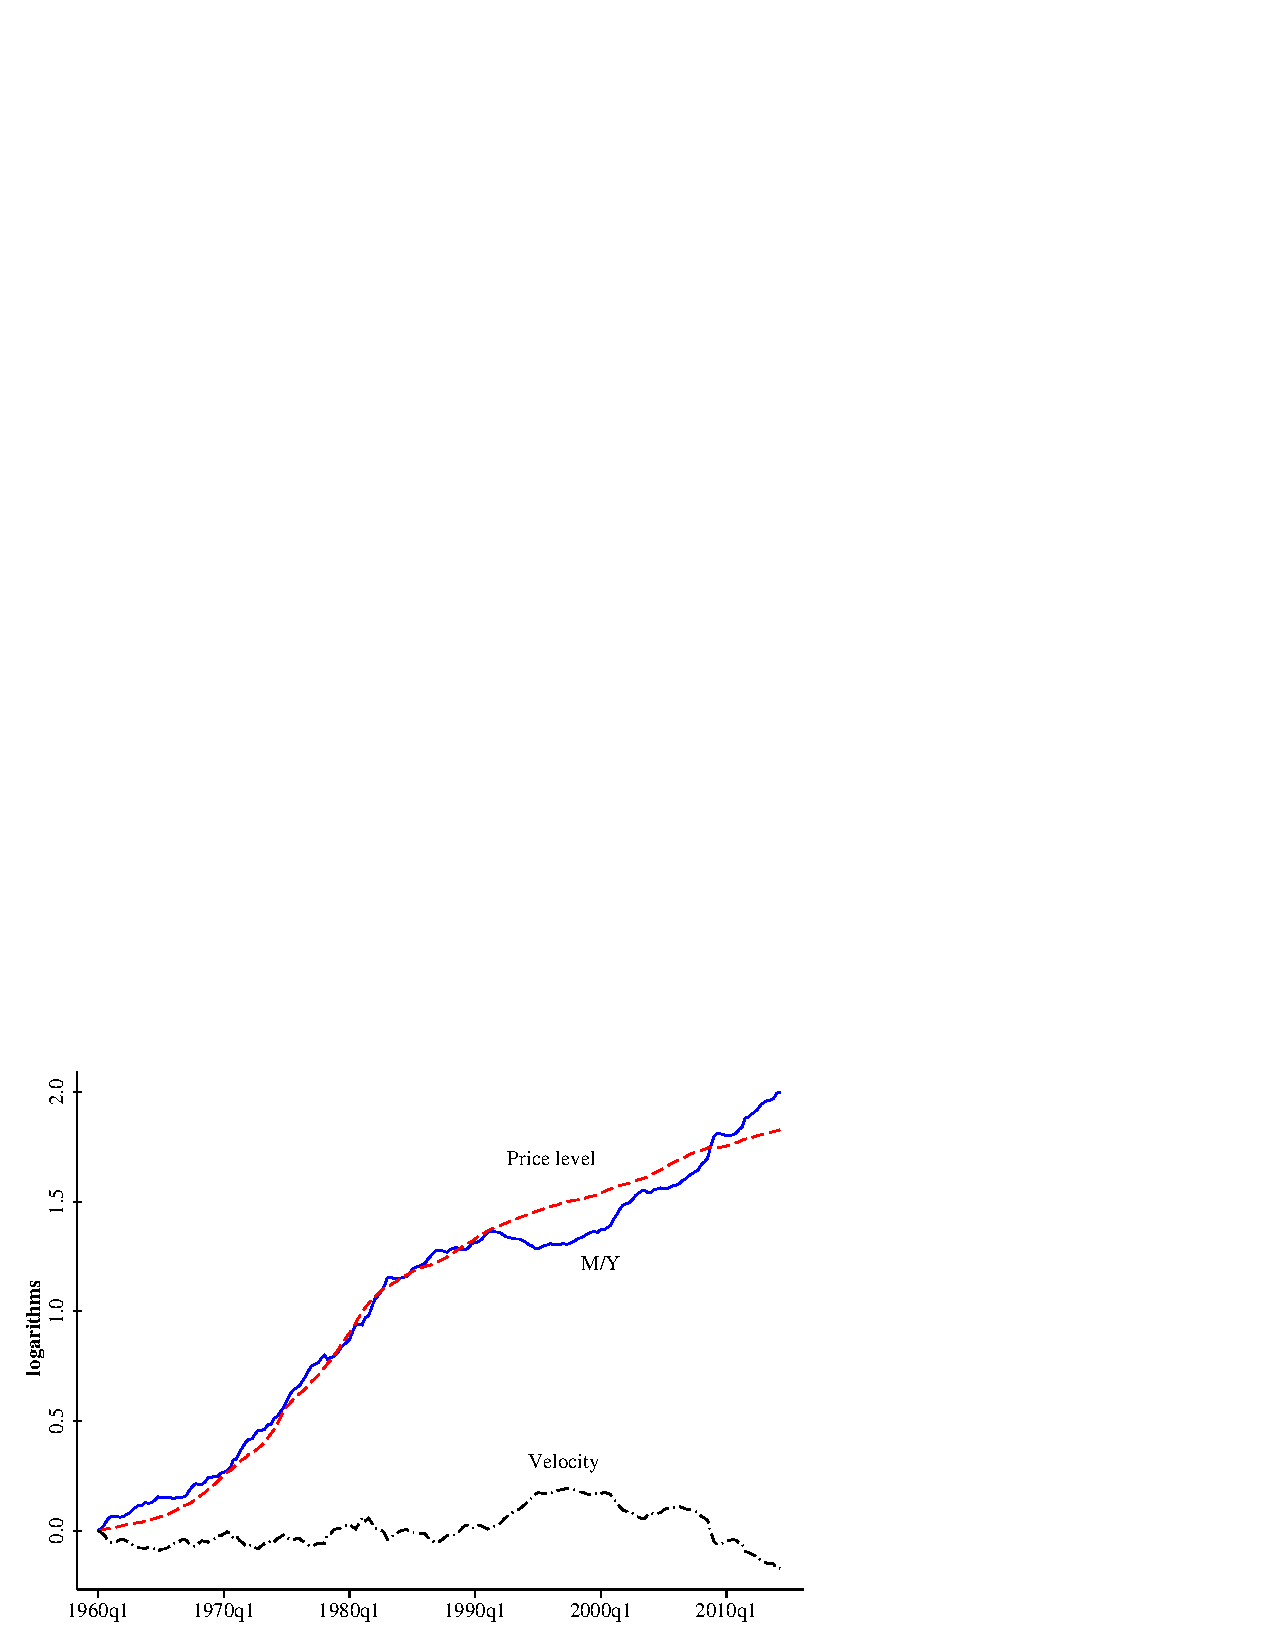
\includegraphics[width=0.8\textwidth]{\figpath Figures/long.pdf}
\end{figure}
%

The short-run evidence for the quantity theory is much weaker.
When we look at year-on-year growth rates,
as we do in Figure~\ref{fig:quantity_short},
we see that velocity has as much short-run volatility as $M/Y$.
As a consequence,
movements in prices are virtually unrelated to movements in money.
To put it bluntly, the quantity theory is a poor guide to short-run fluctuations
in inflation\index{inflation} rates.\index{quantity theory of money|)}

%We'll discuss the short run later in the course, where we try to
%figure out the impact of monetary policy on real output,
%inflation, and interest rates.

\begin{figure}[ht]
    \caption{The quantity theory in the short run.}
    \label{fig:quantity_short}
    \centering
    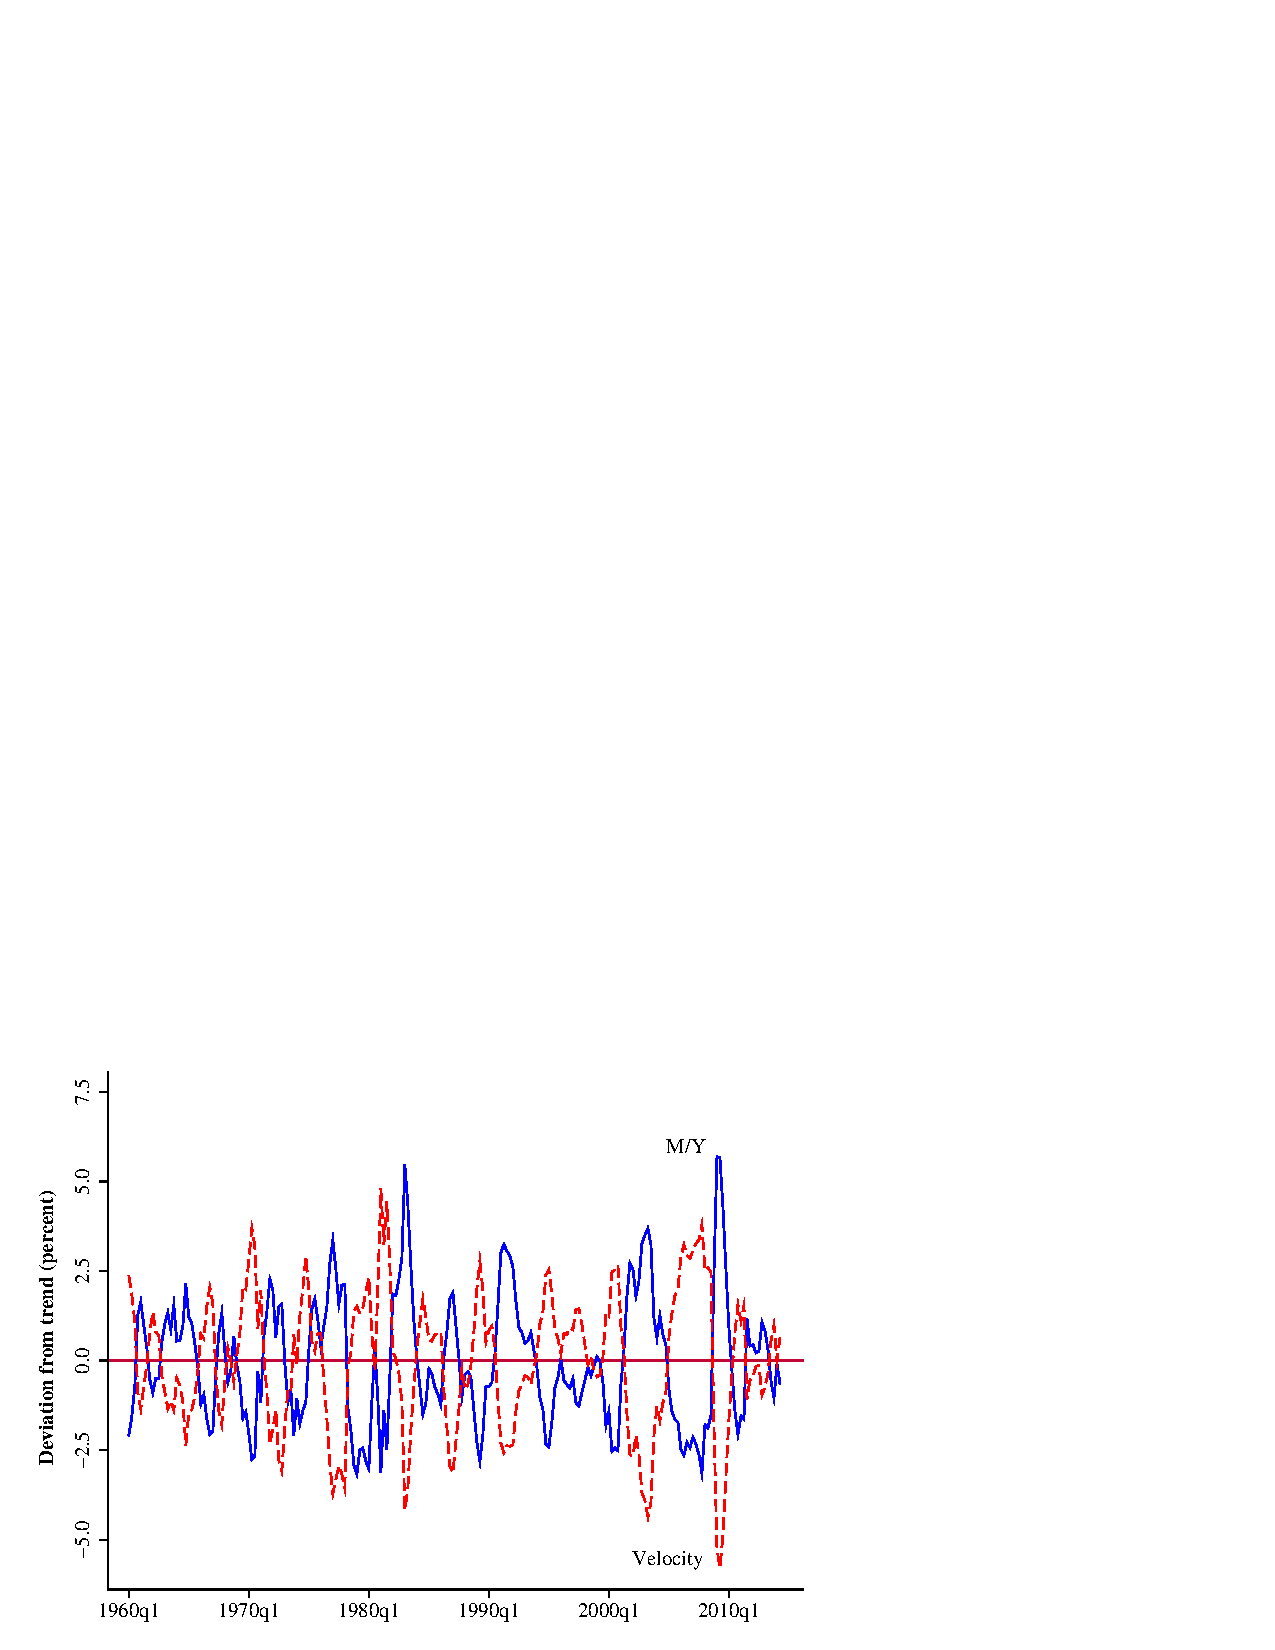
\includegraphics[width=0.8\textwidth]{\figpath Figures/short_1.pdf}
\end{figure}

% ?? change to year-on-year growth rates


\section{Changing the money supply\index{monetary policy!money supply}}

Currency is a liability of the government,
which can (and does) change the quantity in circulation.
To see how this works, it's helpful to take a
step back and consider the broader issue of government debt.
We can divide the government's debt management into two
related pieces.
The first piece is the size of the debt.
Measured in units of currency (dollars, say, or pesos),
the debt changes over time as the government runs surpluses
or deficits.
Mathematically, we might write:
\begin{eqnarray*}
    \mbox{Debt}_{t} &=& \mbox{Debt}_{t-1} + \mbox{Deficit}_t .
\end{eqnarray*}
This is an example of a government budget constraint, something
we'll see more of later on.\index{government budget!budget constraint}
The second piece is the composition of the debt.
In practice, governments have many different liabilities,
but for the purposes of this discussion, let us say, it has two:
government bonds \index{bond} and money (currency).
In both theory and practice,
these two pieces are typically separate,
with the treasury issuing bonds \index{bond} to cover the entire debt
and the monetary authority (central bank \index{central bank|(textbf}) buying back
some of these bonds \index{bond} and issuing money in return.

Day-to-day monetary policy in most countries consists of what we term
{\it open-market operations\/}:  purchases or sales of
government debt (bonds\index{bond}).
At any point in time, the treasury's balance sheet looks
something like:
%\begin{center}
%\begin{tabular}{lr|lr}
%\multicolumn{4}{l}{Central bank \index{central bank}} \\
%\hline
%Assets\phantom{ities} &\phantom{100}&  Liabilities \\
%\hline
%bonds \index{bond} &  100 & Money & 100
%\end{tabular}
%\end{center}
%
\begin{center}
\begin{tabular}{lr|lr}
\multicolumn{4}{l}{Treasury} \\
\hline
Assets\phantom{ities}  &\phantom{100}&  Liabilities \\
\hline
& & Bonds & 200
\end{tabular}
\end{center}
%
and the central bank's  looks like:
%
\begin{center}
\begin{tabular}{lr|lr}
\multicolumn{4}{l}{Central bank} \\
\hline
Assets\phantom{ities}  &&  Liabilities \\
\hline
Bonds &  100 & Money & 100
\end{tabular}
\end{center}
%
If it seems strange to treat money as a liability of the
central bank (isn't money an asset?),
think of it as a bond \index{bond} with the unusual
feature that its nominal interest rate is zero.
That's what it is, which makes it a good deal for the borrower.\index{interest rate!nominal|(}

An open-market purchase of bonds \index{bond} results in an increase
in bonds \index{bond} held by the central bank and an equal increase in its
monetary liability.
For example, a purchase of 20 worth, of bonds \index{bond} would change its
balance sheet to:
%
\begin{center}
\begin{tabular}{lr|lr}
\multicolumn{4}{l}{Central bank} \\
\hline
Assets\phantom{ities}  &&  Liabilities \\
\hline
Bonds &  120 & Money & 120
\end{tabular}
\end{center}
%
The result is an increase in the amount of money in private hands,
since the private sector (the other side of this transaction)
has reduced its holdings of government bonds \index{bond}
and increased its holdings of money.
Similarly, an open-market sale of bonds \index{bond} would reduce the amount of money in
private hands.

The question we're leading up to is why money growth is so high
in countries with big inflations.
Why does the central bank keep issuing money?


\section{Big Inflations}

If inflation\index{inflation} is as easily cured as Friedman suggests
(``control the money supply''),
why do big inflations happen?
People who live through such
episodes describe them as traumatic; they spend an hour or more
every day converting cash into anything with stable value:  real estate,
cars, foreign assets.
The economy is usually a mess, but whether that is cause or effect is
hard to say.
But if big inflations are so painful, why do governments let them happen?
The problem, typically, starts with a government deficit.\index{government budget!budget deficit@budget (or government) deficit}
A political impasse makes it nearly impossible to reduce the deficit.
Given the government's budget constraint, it must then issue debt.
There is apparently no shortage of ready buyers of US debt
(ditto other developed countries),
but the same can't be said for every country.
If no one will buy its debt,
the only remaining option is to finance the deficit with money
(read: oblige the central bank to purchase bonds\index{bond} from the treasury).
In short, when the government can't
pay its bills in any other way, it pays them with money, which is
easy enough to print.
The effect of this, of course, is inflation.\index{inflation}\index{government budget!budget constraint}

The impact here of fiscal policy (government deficits) on inflation
is referred to as fiscal dominance, because fiscal policy dominates monetary policy.
Nobel Prize-winner Thomas Sargent \index{Sargent, Thomas} and his co-author, Neil Wallace,
described a stark version of this.
They showed that even a central bank that aims for low inflation will fail
if the government issues debt without end.
Think of the problem\index{time consistency} as
a version of the \hyperref[sec:time_cons]{time-consistency problem}\index{time consistency}
discussed in Chapter \ref{chp:insp}.
If everyone knows that the central bank eventually will be compelled to print money
to avoid outright default by the government, inflation expectations
 will rise today despite the central bank's \index{central bank|)} caution. The key is
 that the bank cannot credibly commit to limit future money creation, while
 expectations of the future drive price setting today.

The conventional solution to ending a big inflation\index{inflation} has two parts.  The
first is fiscal discipline: Balance the government budget.  The
second is monetary discipline: Separate the central bank
from the treasury and tell the bank that its job is to maintain
price stability. Though there are many fine points --- how quickly must
the deficit be eliminated?  should the IMF supply short-term
financing?  --- the outlines of the problem and its solution
are clear.\index{government budget!budget deficit@budget (or government) deficit}
%Brazil managed to bring inflation under control by tightening its budget.
Going back to Friedman's quote: Inflation may be a monetary phenomenon,
but the trouble often starts with fiscal policy and the political situation that led to it.
When fiscal imperatives drive monetary policy ---
like the fiscal dominance in the Sargent and Wallace analysis ---
inflation eventually follows.

For someone operating an international business,
the thing to remember is that ``big inflations''
are relatively common.
What do you do if you're hit with one?
You'll probably find that the
most important thing you can do is streamline your cash management.
If you can reduce the payment
terms from (say) 60 days to 30 days, you increase your ``real'' revenue substantially.
You may also find that big inflations\index{inflation} lead to policies --- such as price controls and capital controls   --- that make life more complicated.
Finally, you may find that your financial statements
are highly misleading, since they measure performance in terms of the local
currency, the value of which is changing rapidly.
For a US subsidiary, high inflation triggers a change
in the rules for translating financial entries into dollars for tax and reporting purposes.

\section{Inflation and interest rates}

The interest rates we typically use are nominal: They tell us how much money we get in the future
for a given investment of money today.\index{interest rate|(textbf}
Since inflation\index{inflation} measures the change in the value
of money, it shows up in interest rates.
More concretely, we would say that the nominal interest
rate equals the real interest rate (the interest rate
adjusted for inflation) plus \textit{expected} \index{inflation!expected inflation}
inflation:
\begin{eqnarray}
    i_t &=& r_t + \pi_t^e .
    \label{eq:mpin_fisher}
\end{eqnarray}
For a given real interest rate $r$,
an increase in expected inflation raises the nominal interest rate
one for one.\index{interest rate!real}


Here is the deeper explanation behind equation (\ref{eq:mpin_fisher}).
Consider a one-year interest rate on a Treasury bill. \index{Treasury!Treasury bill}
The rate tells us how many dollars (say)
we get in one year for a given payment of dollars today.
For example, if a 12-month treasury bill has a price
of \$96.15, its annualized yield \index{bond!bond yield}
 is the value of $i$ that solves
%
\begin{eqnarray}
    96.15 &=& \frac{100}{1+i_t}.
    \label{eq:nominal_yield}
\end{eqnarray}
%
In this case, $i_t = 4$ percent.  Thus, each dollar invested today gives us
1.04 dollars in 12 months.
We refer to $i_t$ as the  {\it nominal rate of interest\/} --- nominal because its refers to payments of currency.

For many purposes, we'd like to know not only the dollar yield, but
also how much 1.04 dollars will buy when we get it.  If we expect
the inflation\index{inflation} rate to be 3 percent a year, then we'd guess that three quarters of the
interest will be eaten up by inflation.  The investment gains
us only about one percent in terms of purchasing power.
We refer to the increase in purchasing power as the
{\it real rate of interest\/} --- real because it refers to the
quantity of real consumption it finances.
That gives us equation (\ref{eq:mpin_fisher}).\index{interest rate!real}


We can show this more formally
by translating the words into equations more carefully.
We have just argued that investors are interested not in the money the
bond \index{bond} is a claim to, but in what that money will buy. If by ``what
that money will buy,'' we mean the basket of goods used to construct
the CPI, we can define the real interest rate $r$ as
%
\begin{eqnarray*}
    (96.15/P_t) &=& \frac{100/ P_{t+1}}{1+r_t},
\end{eqnarray*}
%
where $P_{t}$ is the CPI index in year $t$ and $P_{t+1}$ is the
expected value of the same index in year $t+1$. What we are doing
here is expressing the current bond \index{bond} price, measured in terms of what
it will buy, as the discounted value of the principal, also measured
in terms of what it will buy. Doing a little algebra, we find
%
\begin{eqnarray*}
    (1+r_t)(P_{t+1}/P_{t}) &=& 100/96.15.
\end{eqnarray*}
%
Then, equation (\ref{eq:nominal_yield}) tells us that the real and
nominal interest rates are related by
\begin{eqnarray*}
    1 + i_t   &=& (1+r_t)(1+\pi_{t}^e),
\end{eqnarray*}
where $(P_{t+1}-P_t)/P_t $ is the expected inflation rate between
$t$ (now) and $t+1$ (a year from now). Since the product
$r_{t}\pi_{t}^e$ is a small number when expected inflation is low, it follows that
\begin{eqnarray*}
    i_t  &\approx&  r_t + \pi_{t}^e, \ \mbox{for \ small \ values \ of \ $r$ and $\pi_{t}^e$},
\end{eqnarray*}
where $\approx$ means ``equals approximately.''
If we're careful about timing, we see that all three variables
are comparisons between now and one year from now.
Inflation is, therefore, typically understood to be
expected inflation,\index{inflation} since we don't know what inflation
will be when we buy the bond\index{bond}.
In principle, we could also take into account the risk
inherent in inflation --- but we won't.


Now that we're done with definitions, we can ask how inflation
affects nominal interest rates.
In principle, either component (the real rate or expected inflation)
can change the nominal interest rate.
In practice, we typically find that in periods of
high and variable inflation,\index{inflation}
the inflation component dominates.
This is approximately true of the US, where high-inflation periods
(the 1970s and early 1980s)
are high-interest-rate periods, too.
It's even more evident in countries with very high inflation rates.


\section{Velocity reconsidered\index{velocity of money}}

In very-high-inflation environments,
people often find that the inflation\index{inflation} rate accelerates
quickly, often far exceeding the rate of money growth.
One factor here is velocity, which typically
rises sharply with inflation.
Why?
Because inflation (and nominal interest) is effectively a tax on holding money:
The higher the tax, the less money you hold.
During big inflations,
people spend money as soon as they get it, because its
value falls by the minute.
It's common, for example, for people to buy groceries
and gasoline as soon as they get their paychecks;
if they wait even a day or two, their purchasing power falls.

If velocity $V$ rises with inflation\index{inflation}, then we can reconsider
\begin{eqnarray}
    \gamma_M + \gamma_V  &=&  \pi + \gamma_Y .
\end{eqnarray}
If $\gamma_Y$ is approximately constant,
then an increase in money growth not only
produces inflation directly, but
its impact is also magnified by the increase in the
interest rate, which increases velocity ($\gamma_V > 0$).
Similarly, when hyperinflations are reversed,
we often see a larger drop in inflation\index{inflation}
than in money growth, as velocity falls.


\section*{Executive summary}

%\setlength{\leftmargini}{.5\oldleftmargini}
\begin{enumerate}
\item Over long periods of time, inflation is closely related to money growth.

%\item High inflation is usually associated with
%high (nominal) interest rates.

\item Extremely high rates of inflation\index{inflation} are invariably associated with high rates of money growth.

\item High money growth is often the result of financing large fiscal deficits with money.
    The deficits, in turn, often reflect some kind of political gridlock.

\item High inflation is typically associated with high interest rates,
since investors demand higher yields \index{bond!bond yield}
 to compensate for the loss of purchasing
power of the currency.
\end{enumerate}
%\setlength{\leftmargini}{\oldleftmargini}

\section*{Review questions}

%\setlength{\leftmargini}{.5\oldleftmargini}
\begin{enumerate}
\item Policy rule.  Friedman suggested that the Fed might do better to adopt
a rule in which it kept the growth rate of the money supply constant.
\begin{enumerate}
\item If the growth rate of real GDP is 3 percent, on average,
what growth rate of the money supply would deliver
average inflation of 2 percent?
\item What are the strengths and weaknesses of such a policy rule?
\end{enumerate}

Answer.
\begin{enumerate}
\item If velocity is constant, then
equation (\ref{eq:quantity_theory-growth}) gives us
a money growth rate of
\begin{eqnarray*}
    \gamma_M &=& \pi + \gamma_Y
            \;\;=\;\;  2 + 3 \;\;=\;\; 5.
\end{eqnarray*}
In words: Money growth accommodates inflation\index{inflation} and economic growth.
\item Strengths: predictable, good average inflation performance,
avoid major policy mistakes.
Weakness: no room for policy to respond to current conditions.
Compare, for example, policy in the aggregate supply (AS) \index{aggregate supply (AS)}
 and demand model
(coming up).
\end{enumerate}


\item Central bank independence.
Why do many countries make central banks \index{central bank} independent of the treasury?

Answer.  The idea is that monetary policy should focus on good long-term
performance and, to accomplish this, should be immune to
short-term political pressure.
With respect to hyperinflations,
you might argue that if the government does not have access to money finance,
it will be forced to confront its deficit issues earlier,
which is a good thing.



\item Zimbabwe.
Zimbabwe ended its hyperinflation by abandoning its currency.
Even official transactions were switched to either US dollars or
    South African rand.
    Does this seem like a good solution?
    Does it make sense for a country to abandon its currency?

Answer.  There's a long tradition of each country having its own currency,
but there's good reason to think at least some countries would be better
off using someone else's.
Zimbabwe has shown no ability to manage it's own currency effectively,
so using another sounds like a move in the right direction.
There are other examples --- Panama and Ecuador use the US dollar --- and perhaps there should be more.

\item Interest rates and inflation.  Go to
\href{http://research.stlouisfed.org/fred2/}{FRED} and find
the three-month treasury bill rate (TB3MS)
and the consumer price index \index{price index!consumer price index (CPI)}
 (CPIAUCSL).
Manipulate them as needed and graph
the nominal interest rate and inflation rate together.
What do you see?

Answer.  Do it and see!\index{interest rate|)}\index{interest rate!nominal|)}

\end{enumerate}
%\setlength{\leftmargini}{\oldleftmargini}


\section*{If you're looking for more}

%Similar material is covered in most macroeconomics textbooks.
Wikipedia has a nice article on hyperinflation,
including a list of the biggest ones of all time.
%
Steve Hanke and Nicholas Krus survey the compete history of
hyperinflation in
``\href{http://www.cato.org/publications/working-paper/world-hyperinflations}{World Hyperinflations}.''
Search:  ``hanke krus hyperinflation.''
Two really good (but more technical) pieces about specific episodes are
Thomas Sargent,
``\href{http://www.nber.org/chapters/c11452.pdf}{The ends of four big inflations},''
and Thomas Sargent and Joseph Zeira,
``\href{http://www.sciencedirect.com/science/article/pii/S1094202511000147}
{Israel 1983}.''


\section*{Symbols and data used in this chapter}

\begin{table}[H]
\centering
\caption{Symbol table.}
\begin{tabular*}{0.8\textwidth}{l@{\extracolsep{\fill}}l}
\toprule
Symbol & Definition\\
\midrule
$M$            &Money stock\\
$V$            &Velocity of money\\
$P$            &Price level\\
$Y$            &Real output or GDP\\
$\ln$        &Natural log\\
$\gamma_x$    &Continuously compounded growth rate of $x$\\
$\pi$         &Inflation ($= P$)\\
$\pi^{e}$    &Expected Inflation\\
$i$            &Nominal interest rate\\
$r$            &Real interest rate ($= i- \pi^e$)\\
\bottomrule
\end{tabular*}
\end{table}

\begin{table}[t]
\centering
\caption{Data table.}
\begin{tabular*}{0.8\textwidth}{l@{\extracolsep{\fill}}l}
\toprule
Variable & Source\\
\midrule
Nominal GDP                    &GDP\\
M2 monetary aggregate        &M2SL\\
M2 velocity                    &M2V\\
Consumer price index
        &CPIAUCSL\\
\bottomrule
\addlinespace
\end{tabular*}
\begin{minipage}{0.8\textwidth}
\footnotesize{To retrieve the data online, add the identifier from the source column to \url{http://research.stlouisfed.org/fred2/series/}.  For example, to retrieve nominal GDP, point your browser to \url{http://research.stlouisfed.org/fred2/series/GDP}}
\end{minipage}
\end{table}

%%%%%%%%%%%%%%%%%%%%%%%%%%%%%%%%%This could cause problems later!%%%%%%%%%%%%%%%%%%%%%%%%%%%%%%%%%%%%%%%%
%%KR: the last table ends up on its own page, but vertically centered.  To force the table to the top, I've
%%added these two aweful lines below.
\vfill
\phantom{x}
%%%%%%%%%%%%%%%%%%%%%%%%%%%%%%%%%%%%%%%%%%%%%%%%%%%%%%%%%%%%%%%%%%%%%%%%%%%%%%%%%%%%%%%%%%%%%%%%%%%%%%%%% 
\chapter{Aggregate Supply and Demand}\label{chp:asad}
\hypertarget{asad}{}

%No extra line here.
\textbf{Tools:} Aggregate supply and demand (AS/AD) graph.

\textbf{Key Words:} Short- and   long-run aggregate supply; sticky wages; aggregate demand; supply and demand shocks; Keynesian.

\textbf{Big Ideas:}
%\vspace{-0.1in}
\begin{itemize}
    \item The AS/AD model relates output and prices in the short and long runs. The model is composed of (i) an upward-sloping short-run aggregate supply curve, which inherits its shape from sticky wages; (ii) a vertical long-run aggregate supply curve; and (iii) a downward-sloping aggregate demand curve.
    \item Shocks to the aggregate supply and demand curves have different effects on inflation and output.
\end{itemize}

\rule{\textwidth}{1pt}

We've seen that economic fluctuations follow regular patterns
and that these patterns can be used to forecast the future.
For some purposes, that's enough.
But if we want to make sense of analysts' discussions of business conditions,
of monetary policy,
or of situations that don't fit historical patterns,
we need a theoretical framework.
The aggregate supply and demand model is the analyst's standard,
the implicit model behind most popular macroeconomic analysis.
It's not the answer to all questions,
but it's a useful tool for organizing our thoughts.
Think of these notes as the executive summary;
textbooks devote hundreds of pages to the same topic.
If you'd like to go deeper, see the references at the end of this chapter.

We take one common shortcut.
In our theory, the variables are real output and the price level.
In practice, we refer to output growth and inflation.
There's a modest disconnect here between theory and practice,
but it's something that can be worked out.
You can thank us later for saving you the trouble of
doing it explicitly.


\section{Aggregate supply\index{aggregate supply (AS)|(textbf}}

The standard business-cycle model used by analysts
is an adaptation of the supply and demand diagram.
We refer to the curves as aggregate supply and aggregate demand to emphasize that we're talking about the whole economy
rather than a single market --- and to remind ourselves that the analogy with supply and demand
in a single market is imperfect.
Figure \ref{fig:asad} is an example.
The aggregate supply (AS) curve  represents combinations of
output (real GDP, which we denote by $Y$) and the price level
(an index $P$ such as the GDP deflator)
consistent with the decisions of producers and sellers (``supply'').
The aggregate demand (AD)\index{aggregate demand (AD)}
 curve represents combinations of output and the price
level consistent with the decisions of buyers (``demand'').

Here's how aggregate supply works.
%How do workers and firms decide how much to work and produce?
We start with the production function,
\begin{eqnarray}
    Y &=& A K^\alpha L^{1-\alpha} ,
    \label{eq:pf}
\end{eqnarray}
where (as usual) $Y$ is output, $A$ is total factor productivity,
$K$ is the stock of physical capital\index{capital!physical capital} (plant and equipment),
$L$ is labor, and $ \alpha = 1/3$.
%Everything but $\alpha$ can in principle change with time $t$.

In the simplest ``classical'' theory, $Y$ is fixed
because nothing on the right-hand side of (\ref{eq:pf}) changes in the short run.
Although current productivity $A$ and capital $K$ can change over time,
we often assume that their current values are set --- that is
they can't be changed by current decisions.
Capital, for example, takes time to produce:
We can increase next year's capital stock by investing today,
but today's capital stock is whatever we happen to have.
Labor $L$ is determined by supply and demand in the labor market,
which gives us a level of work that reconciles firms'
demand with individuals' supply.
The result is a vertical aggregate supply curve, such as AS$^*$ in the figure,
in which output does not depend on the price level $P$.


%%%%%%%%%%%%%%%%%%%%%%%%%%%%%%%%%%%%%%%%%%%%%%%%%%%%%%%%%%%%%%%%%%%%%%%%%%%%
%  Supply and demand diagram
\begin{figure}[ht]
\caption{Aggregate supply and demand.}
\label{fig:asad}
%
\centering
\setlength{\unitlength}{0.075em}
\begin{picture}(250,200)(0,0)
%\footnotesize
\thicklines

% horizontal axis
\put(-30,0){\vector(1,0){300}}
\put(255,-16){$Y$}
\put(142,-16){$Y^*$}

% vertical axis
\put(0,-20){\vector(0,1){200}}
\put(-15,155){$P$}

% demand
\put(25,165){\line(4,-3){200}}\put(230,10){AD}

% supply
\put(25,13){\line(4,3){200}} \put(230,160){AS}
\put(146.4,0){\line(0,1){170}} \put(138,175){AS$^*$}

% equilibrium labels
\put(105,85){\footnotesize A}
\put(135,60){\footnotesize B}
%\put(138,64){\footnotesize C}
% dotted lines
%\qbezier[31]{(133,0)(133,46)(133,92)}
%\qbezier[45]{(0,92)(67,92)(133,92)}
%\qbezier[45]{(0,72)(67,72)(133,72)}
\end{picture}
\begin{minipage}{0.7\textwidth}
\vspace{0.45in}
\footnotesize{The horizontal axis is real GDP;
the vertical axis is the price level.
The lines represent aggregate supply
 (two versions, AS and AS$^*$)
and demand (AD).}
\end{minipage}

\end{figure}

%%%%%%%%%%%%%%%%%%%%%%%%%%%%%%%%%%%%%%%%%%%%%%%%%%%%%%%%%%%%%%%%%%%%%%%%%%%%

A vertical aggregate supply curve was the state of the art until the 1930s,
when John Maynard Keynes\index{Keynes, John Maynard}
(pronounced ``canes'')
decided that the Depression demanded a new theory.
He and his followers (the ``Keynesians'')
argued that the aggregate supply curve should be upward-sloping.
Why?  The most popular argument is that wages or prices are ``sticky'':
They do not adjust quickly enough
to equate supply and demand for labor or goods. One version of this story is that
wages are sticky downward (that is, wages generally don't fall when
demand for labor declines).
The sticky wage\index{sticky wages}
 analysis goes something like this:
If the nominal wage $W$ is fixed (i.e., very sticky),
then an increase in the price level reduces the real wage $W/P$,
making labor more attractive to firms, who hire more workers,
which raises output.
(That is, we continue to use the labor demand curve.)

The Keynesian sticky wage/price story leads to
an aggregate supply curve that is upward-sloping,\index{sticky prices}
since an increase in the price level leads to a lower
real wage and, therefore, more people hired by firms.
We refer to it as the short-run aggregate supply\index{aggregate supply (AS)!short-run aggregate supply|textbf}
 curve, because wages and prices are not thought to be sticky forever.
Eventually they adjust, putting us on the vertical aggregate
supply curve AS$^*$, which we refer to as long-run aggregate supply\index{aggregate supply (AS)!long-run aggregate supply|textbf}.


That's what aggregate supply looks like,
but what kinds of things make it shift over time?
Here's a list:
%
\begin{itemize}
\item Productivity:  An increase in $A$ shifts AS to the right.
You can see why from the production function (\ref{eq:pf}) --- an increase in productivity $A$ raises output $Y$.


\item Capital:  ditto an increase in $K$.
\item Price of imported oil:  This is a more subtle one, but
an increase in the price of oil works like a negative productivity shock
in an oil-importing country like the US and shifts AS to the left.
Why?  Because production involves energy, as well as capital and labor, as an input.
In our measurement system, GDP consists only of value added by capital
and labor.
If the price of oil rises, then a larger fraction of total production
is paid to oil producers, leaving less for capital and labor and, therefore, reducing GDP.
There's very little question that this is what happens in practice: An increase in the price of oil leads to larger payments to oil producers
and smaller payments to capital and labor.
Oil producers benefit; oil consumers do not.
\end{itemize}
%
To simplify matters, we'll assume that these factors shift both AS and AS$^*$
left or right by the same amount.
%We could consider alternatives, but we won't.
%Trust me, it's not worth the effort.
% ?? think about this


\section{Aggregate demand \index{aggregate demand (AD)|(textbf}}

% QT first?

The primary role of the Keynesian aggregate supply curve is to
allow demand to influence output;
if supply is vertical, then changes in demand affect the price level,
but not output.
That's what we assumed when we discussed the quantity theory --- that changes in the money supply affect prices, but not output.
But if aggregate supply is flatter,
shifts in demand affect both prices and output.

But what is the aggregate demand curve and where does it come from?
Recall that aggregate demand
 refers to the purchase of goods and services.
The aggregate demand
 curve tells us how much demand for output
there is at each price level.

The simplest version follows from the quantity theory,
\begin{eqnarray}
    M V &=& P Y ,
    \label{eq:qt}
\end{eqnarray}
which you might recall from Chapter \ref{chp:mpin}.
The aggregate demand
 curve is the relation between $P$ and $Y$ for a
given supply of money $M$,
determined presumably by the monetary authority.
For simplicity, we will assume that velocity $V$, is constant.
That gives us an inverse relation between $P$ and $Y$,
as shown in Figure \ref{fig:asad}.
Changes in $M$ lead to shifts in AD.
If we increase $M$, then we need either an increase in output $Y$
or an increase in the price level $P$ to satisfy (\ref{eq:qt}),
so AD shifts up or to the right.

There's a more complex version in which monetary policy operates
through the interest rate.
The idea is that an increase in the money supply reduces
the interest rate,
which stimulates interest-sensitive components of demand,
such as business investment and housing.\index{interest rate}

Other movements in aggregate demand
 come from the expenditure components:
demand by consumers ($C$); firms ($I$); government ($G$);
and the rest of the world ($\NX$).
You often read, for example, that high demand by consumers
leads to higher output --- more on this shortly.
Ditto increases in government purchases
(wars are the biggest examples historically)
and investment by firms (remember, investment is the most volatile
expenditure component).
Keynes thought investment fluctuations stemmed,
in part, from the ``animal spirits'' of business people,
which you might think of as shifts in investment demand
driven by psychological factors.\index{interest rate}


%Our guess is that this leaves you breathless.
%That's ok, our goal was to skim over the details.
%Just take our word for it that aggregate demand (AD) \index{aggregate demand (AD)}
% involves an
%inverse relation between the price level and output,
%and that a variety of obvious things increase demand:
%increasing the supply of money, government purchases,
%and so on.

Let's summarize.
The aggregate demand
 curve is downward-sloping, reflecting
the decline in the real money supply as the price level increases.
The following factors (``shocks'')
shift the aggregate demand curve to the right:
%
\begin{itemize}
\item An increase in the supply of money.
\item An increase in government purchases.
\item An increase in consumer demand:  For given levels of income,
consumers decide to spend more.
\item An increase in investment demand:
For given levels of interest rates and output,
firms decide to invest more (animal spirits).
\end{itemize}

\section{Aggregate supply and demand together}

Now let's put supply and demand together.
Equilibrium \index{equilibrium}
 is where supply and demand cross.
The only difference in this respect from
the traditional supply and demand analysis is that we have two
supply curves.
The short-run equilibrium
 is where AD and AS cross.
The long-run equilibrium is where AD and AS$^*$
 cross.

Here's how that works.
The short-run equilibrium is where aggregate supply
 AS and aggregate
demand AD cross:  the point labeled A in Figure \ref{fig:asad}.
In this example, the economy's output is below its long-run
value $Y^*$, indicated by AS$^*$.
The reason is that the real wage is too high, leading firms to demand
less work than individuals would like to offer at the going real wage.

The long-run equilibrium is where aggregate demand
 AD crosses long-run aggregate supply\index{aggregate supply (AS)!long-run aggregate supply}
 AS$^*$:  point B in the figure.
How do we get there?
Eventually, the real wage adjusts (either $W$ falls or $P$ rises),
shifting the AS curve down, until
we get to the point where AD crosses the long-run aggregate supply.\index{aggregate supply (AS)!long-run aggregate supply}

%Curve AS$^*$.
%The dynamics are governed by the speed of adjustment \index{speed of adjustment}
% of wages.
%[Suggestion: show in the figure how AS shifts until we reach B.]


%%%%%%%%%%%%%%%%%%%%%%%%%%%%%%%%%%%%%%%%%%%%%%%%%%%%%%%%%%%%%%%%%%%%%%%%%%%%
%  Supply and demand diagram
\begin{figure}[!ht]
\caption{The impact of an increase in the money supply.}
%
\centering
\setlength{\unitlength}{0.075em}
\begin{picture}(250,200)(0,0)
%\footnotesize
\thicklines

% horizontal axis
\put(-30,0){\vector(1,0){300}}
\put(255,-16){$Y$}
\put(142,-16){$Y^*$}

% vertical axis
\put(0,-20){\vector(0,1){200}}
\put(-15,155){$P$}

% demand
\put(25,165){\line(4,-3){200}}\put(230,10){AD}
\put(65,165){\line(4,-3){200}}\put(270,10){AD$'$}

% supply
\put(25,13){\line(4,3){200}} \put(230,160){AS}
%\put(65,13){\line(4,3){200}} \put(270,160){AS$'$}
\put(146.4,0){\line(0,1){170}} \put(138,175){AS$^*$}

% equilibrium labels
\put(105,85){\footnotesize A}
\put(150,115){\footnotesize B}
%\put(138,64){\footnotesize C}
% dotted lines
%\qbezier[31]{(133,0)(133,46)(133,92)}
%\qbezier[45]{(0,92)(67,92)(133,92)}
%\qbezier[45]{(0,72)(67,72)(133,72)}

\end{picture}
\begin{minipage}{0.7\textwidth}
\vspace{0.45in}
{\footnotesize Aggregate demand
 AD shifts right to AD$'$,
moving the short-run equilibrium from A to B.}
\end{minipage}
\label{fig:asad_m}
\end{figure}
%%%%%%%%%%%%%%%%%%%%%%%%%%%%%%%%%%%%%%%%%%%%%%%%%%%%%%%%%%%%%%%%%%%%%%%%%%%%


Let's put our theory to work:

\textbf{What is the impact of an increase in the supply of money?}
Consider a short-run equilibrium at a point like A in Figure \ref{fig:asad_m}.
Could the monetary authority do something to raise output to its long-run
level?
An increase in the money supply will shift AD to the right,
as in the new aggregate demand curve AD$'$.
If we increase the money supply by the right amount,
we can establish a new
equilibrium at B, where output is exactly its long-run value.
[We recommend that you work through all these shifts of curves on your own
to make sure you follow the argument.]
How was this accomplished?
The increase in the supply of money increased the price level.
Since the nominal wage is fixed, the real wage falls,\index{sticky wages}
making labor more attractive to firms
and thereby increasing employment and output.

Alternatively, suppose that we're at the long-run equilibrium.
What are the short- and long-run effects of increasing the
money supply?
The short-run impact is to raise prices and output, as
we move up the aggregate supply curve.
[You should work this out yourself in a diagram.]
But the long-run effect is to increase prices,
with no impact on output.
Why?  Because monetary policy doesn't affect
the economy's long-term ability to produce.
That's what we saw with the quantity theory.

\textbf{What is the impact of an increase in government purchases?}
You might recognize this as an example of a stimulus program.
Suppose that we start, as we did above, with output below
its long-term value,
such as point A in Figure \ref{fig:asad_m}.
Then, an increase in government purchases shifts aggregate demand to the right,
 as illustrated in the same figure.

% ?? extensions: timing and g, tax cuts

\textbf{What is the impact of an increase in the price of oil?}
Consider an initial short-run and long-run
equilibrium, such as point A in Figure \ref{fig:asad_oil}.
An increase in the price of oil
shifts the aggregate supply curve to the left.
Remember:  we shift both supply curves horizontally
by the same amount.
The new short-run equilibrium is at point B,
where AD and AS$^{'}$ cross.
Eventually the short-run aggregate supply\index{aggregate supply (AS)!short-run aggregate supply}
 curve shifts until it crosses AD at AS$^{*'}$, giving us long-run equilibrium at C.


%%%%%%%%%%%%%%%%%%%%%%%%%%%%%%%%%%%%%%%%%%%%%%%%%%%%%%%%%%%%%%%%%%%%%%%%%%%%
%  Supply and demand diagram
\begin{figure}[ht]
\caption{The impact of an increase in the price of oil.}
\label{fig:asad_oil}
%
\centering
\setlength{\unitlength}{0.075em}
\begin{picture}(250,200)(0,0)
%\footnotesize
\thicklines

% horizontal axis
\put(-30,0){\vector(1,0){300}}
\put(255,-16){$Y$}
\put(142,-16){$Y^*$}
\put(102,-16){$Y^{*\prime}$}

% vertical axis
\put(0,-20){\vector(0,1){200}}
\put(-15,155){$P$}

% demand
\put(25,165){\line(4,-3){200}}\put(230,10){AD}
%\put(65,165){\line(4,-3){200}}\put(270,10){AD$'$}

% supply
\put(65,13){\line(4,3){200}} \put(270,160){AS}
\put(25,13){\line(4,3){200}} \put(230,160){AS$'$}
\put(146.4,0){\line(0,1){170}} \put(138,175){AS$^*$}
\put(106.4,0){\line(0,1){170}} \put(98,175){AS$^{*\prime}$}

% equilibrium labels
\put(150,55){\footnotesize A}
\put(122,75){\footnotesize B}
\put(95,94){\footnotesize C}
\put(95,76){\footnotesize D}
%\put(95,54){\footnotesize D}
% dotted lines
%\qbezier[31]{(133,0)(133,46)(133,92)}
%\qbezier[45]{(0,92)(67,92)(133,92)}
%\qbezier[45]{(0,72)(67,72)(133,72)}

\end{picture}
\begin{minipage}{0.7\textwidth}
\vspace{0.45in}
{\footnotesize Aggregate supply
 curves shift left from AS/AS$^*$ to AS$'$/AS$^{*\prime}$,
moving the short-run equilibrium from A to B.}
\end{minipage}

\end{figure}
%%%%%%%%%%%%%%%%%%%%%%%%%%%%%%%%%%%%%%%%%%%%%%%%%%%%%%%%%%%%%%%%%%%%%%%%%%%%

Note that this adverse supply shock reduces output but raises the price level.
People sometimes refer to this combination as ``stagflation,''
a term coined to describe what seemed to be a surprising or implausible outcome.  In fact, it's a natural result of leftward
shifts in the aggregate supply  curve.
Note that ``supply shocks'' are inflationary,
in the sense that they raise the price
level unless something is done to aggregate demand\index{aggregate demand (AD)|)}
 to offset them. \index{supply shocks}

\textbf{Where do business cycles \index{business cycle} come from?}
It's obvious that we can generate economic fluctuations by shifting
the aggregate supply\index{aggregate supply (AS)|)}
 and demand curves around.
Less obvious is what kinds of shifts are most common,
or how they lead to the patterns we see in the data.
As a rule, shifts in AD move price and output in the same direction, while shifts in AS move price and output in opposite directions.
By looking at the statistical relation between prices and output,
we can get a sense of whether supply or demand shifts are more
prevalent.



\section{Beyond supply and demand}

This is a nice model, relatively easy to use,
and applicable to lots of things.
But it's theory, not the real world.
Eliza Doolittle notwithstanding,
it's often a mistake to fall in love with your own creation.
Economists have learned to be humble; some might say that we have a lot to be humble about.

The aggregate supply
 and demand framework can be developed
further, but it has two weaknesses that are hard to overcome.
The first is what we might term general equilibrium:
Many things affect both supply and demand, so it seems
artificial to separate them as we have.
The second is dynamics:  The impact of many shocks depends
not only on what happens now, but also on what we expect to happen
in the future.
That's a hard thing to model explicitly, more so in a single diagram.

Consider the interaction of supply and demand.
If productivity rises, is that a shift of supply or demand?
Obviously it shifts supply:  The production function shifts,
which directly affects producers.
But consumers are also producers.
An increase in productivity  raises wages,
which gives them more income, perhaps
leading them to consume more.
It also raises the demand for capital goods,
since capital is now more productive.
Are these shifts in demand?
In the sense that they change consumption and investment
decisions, the answer is yes.
The closer you look, the harder it is to separate
supply from demand.

Another example is the financial crisis.
Did it shift supply or demand?
Think about it and let us know what you come up with.

Or consider dynamics.
One issue is causality.
Think about popular comments to the effect that
consumer demand is driving the economy.
A journalist might say:  ``High consumer demand led to an economic boom.''
The logic is perfectly consistent with our AS/AD analysis,
but is that really what's going on?
If we think about consumption,
one of our first thoughts should be to think about our future income.
If we expect to have much higher income in the future
(that MBA is really paying off!),
we might consume more now.
But think about what that does to causality. For the economy as a whole, has output gone up because we consumed
more, or did we consume more because we expected output to go up?
It's not easy to tell the difference between the two mechanisms.

Investment is similar.  Firms make investment decisions
based on their assessment (i.e., guess)
of market conditions years down the road.
That's why ``institutions'' are so important. Good institutions give firms some assurance that the rules won't change
in ways that make the investment less attractive.
With respect to business cycles\index{business cycle}, we could ask the same question
we asked of consumption: Did high investment lead to a booming economy,
or did expectations of a booming economy lead to high investment?
If we're forecasting, we may not care, as long as the two go
together.
But if we want to understand what's going on, we need to address
this issue one way or the other.
Fed minutes and analysts' reports
are filled with conjectures over exactly this kind of issue.

A related issue is what we might call context:
the set of assumptions people use to think about
the connection between current and future events.
Monetary policy is a good example.
In most developed countries,
central banks \index{central bank} have worked hard to convince people
that if they increase the money supply now,
it does not signal future increases in the money supply.
If it did, people might immediately demand higher wages,
which would lead to higher prices and inflation.\index{inflation}
But if they regard a current increase in the money supply as temporary,
they might very well be content with wages and prices
where they are.
That's one of the reasons that monetary policy is different
in the US and Argentina:
The contexts for understanding current events are different.
It's also an important practical issue for monetary policy: central banks \index{central bank} must signal not only their current policies,
but their likely future policies.
That's exactly what the Fed is struggling with right now --- how to do that effectively.




\section*{Executive summary}

%\setlength{\leftmargini}{.5\oldleftmargini}
\begin{enumerate}
\item In the long run, output is determined by the production function:
the productivity of the economy and the behavior and institutions
that determine investment and employment.

\item In the short run, output may respond to changes in
aggregate demand (e.g., the money supply) because of sticky wages or prices
or possibly other market frictions.

\item This is theory, not reality.
There's no substitute for adding some common sense.
\end{enumerate}
%\setlength{\leftmargini}{\oldleftmargini}

%\begin{comment}
\section*{Review questions}

%\setlength{\leftmargini}{.5\oldleftmargini}
\begin{enumerate}
\item AS/AD review.  Get out a piece of paper and do the following
without looking at the text:
\begin{enumerate}
\item Draw the aggregate demand
 curve on a piece of paper.
Why does it slope downward?
\item Draw the short-run aggregate supply
 curve on a piece of paper.\index{aggregate supply (AS)!short-run aggregate supply}
Why does it slope upward?
\item Draw the long-run aggregate supply
 curve where the two cross.
Why is it vertical?
\item What happens in the short run if we increase the money supply?
In the long run?
\end{enumerate}

Answer. You may refer to Figure \ref{fig:asad_m}.
\begin{enumerate}
\item The AD curve slopes down because a given quantity of money
can support
a high price level $P$ or high real output $Y$, but not both.
See the quantity theory equation (\ref{eq:qt}).
\item The idea is that a higher price level leads, at a fixed wage rate,
to lower real wages, leading firms to hire more workers and expand output.
\item In the long run, wages adjust, and output and employment do not depend
on the price level.
\item If we increase the money supply, aggregate demand
 shifts to the right.
The immediate impact is to raise output and prices as we move along
the short-run aggregate supply
 curve.\index{aggregate supply (AS)!short-run aggregate supply}
In the long run wages adjust, leading output to revert to its long-run equilibrium
level and prices to rise.

You might notice that the long-run impact duplicates our analysis of hyperinflation,
where money affects prices but not output.
What we've added is the possibility that monetary policy can affect
output in the short run.
\end{enumerate}

\item Supply or demand?
Suppose exports increase sharply.
Is this a shift in supply or demand?

Answer.  The question is whether this has to do with the production (supply)
or purchase (demand) of goods and services.
Exports are sales, so it's a purchase, hence demand.
We would approach it the same way we approached the increase
in the money supply in the previous question.

%\item How does our analysis of the movement from short-run to long-run
% equilibrium change if wages are very sticky?
%
%Answer.  In some countries, institutions can make the wage very slow to adjust.
%In that case, we might expect slower adjustment to the long-run
%level of output.

\item France.
We've seen that the employment ratio is lower in France than in the US.
Should France increase its money supply in an attempt to increase
employment and output?

Answer.  Good question, but the answer is no:
One suspects that the level of employment
associated with the long-run aggregate supply
 curve is lower than
markets would produce on their own.
%Why?
%Because this has been true for decades.
%You might consider using monetary policy to drive output beyond the
%long-run supply curve, but eventually you'll end up back there anyway.
%Put another way:  This is a micro issue and macro policy can't solve it.

\item Causality.
Do increases in consumption cause increases in output,
or the other way around?
That is, could the correlation between consumption and output be because
high output leads consumers to spend more, rather than the reverse?

Answer.  We observe data, not causality,
and we may not be able to distinguish between
alternative causal interpretations of the same events.
That's what makes economic analysis so much fun.
In some cases, we might be able to tell the difference,
and these cases might lead to more general insights.
For example, winning the lottery generates an increase in consumption,
and we can say confidently that the causality runs from
higher income to higher consumption.
Why?  Because the reverse argument is absurd: High consumption didn't cause the person to win the lottery.
In most cases, however,
we can have multiple plausible causal interpretations of events,
and there's not much we can do about it.
\end{enumerate}
%\setlength{\leftmargini}{\oldleftmargini}


\section*{If you're looking for more}

Similar material is covered in greater depth
in most macroeconomics textbooks.

\section*{Symbols used in this chapter}

\begin{table}[H]
\centering
\caption{Symbol table.}
\begin{tabular*}{0.95\textwidth}{l@{\extracolsep{\fill}}l}
\toprule
Symbol & Definition\\
\midrule
$Y$    &Real output (=real GDP)\\
$A$    &Total factor productivity (TFP)\\
$K$    &stock of physical capital  (plant and equipment)\\
$L$    &quantity of labor (number of people employed)\\
$\alpha$     &Exponent of K in Cobb-Douglas production function \\
        &(= capital share of income)\\
$P$    &Price level\\
$Y^*$    &Equilibrium (or potential) output\\
AS    &Short-run aggregate supply (AS)
\\
AS$^*$    &  long-run aggregate supply
 (AS)


\\
AD    &aggregate demand (AD)
\\
AD$'$    &aggregate demand (AD)
 after a shock\\
AS$'$    &aggregate supply (AS)
 after a shock\\
$M$    &Money stock\\
$V$    &Velocity of money\\
$C$    &Private consumption\\
$I$    &Private investment (residential and business investment)\\
$G$    &Government purchases of goods and services (not transfers)\\
$X$    &Exports\\
$M$    &Imports\\
$\NX$    &Net exports ($=X-M$)\\
\bottomrule
\end{tabular*}
\end{table}

\chapter{Policy in the AS/AD model \index{AS/AD model}
}\label{chp:pasad}
\hypertarget{asadpolicy}{}

%No extra line here.
\textbf{Tools:} Aggregate supply and demand (AS/AD) graph.

\textbf{Key Words:} Policy objectives; potential output; output gap.

\textbf{Big Ideas:}
%\vspace{-0.1in}
\begin{itemize}
    \item The objectives of monetary policy are generally thought to be (i)~stable prices and (ii)~output near its long-run equilibrium level.
\item A direct consequence is that monetary policy should respond differently to demand and supply shocks.
As a general rule, policy should resist/offset changes in output triggered by shifts in demand
and accommodate/reinforce changes triggered by shifts in supply.
    \item We can identify supply or demand shocks from whether output and prices move together or in opposite directions.
\end{itemize}

\rule{\textwidth}{1pt}

We've seen that aggregate demand
 and supply can shift on their own or,
sometimes, as a result of changes in policy,
including monetary policy.
But what policy changes are called for?
Should we always shift the aggregate demand
 curve to maintain
low inflation?\index{inflation}  High output?
Are these two objectives in conflict?
The short answer is that we should respond differently to changes in supply and demand.
A somewhat longer answer follows.


\section{Objectives of policy}

The traditional guide to economic policy is the invisible hand.
If markets work well, then we simply leave them to do their job.
If not, we may act to facilitate their operation.
In the aggregate demand\index{aggregate demand (AD)}
 and supply framework,
the idea is that the   long-run aggregate supply \index{aggregate supply (AS)!long-run aggregate supply}\index{aggregate supply (AS)}
 curve is where the uninhibited operation of markets would lead us.
In the short run, sticky wages (or other market imperfections)
may delay the adjustment, but that's
where the invisible hand ultimately would direct us.
One consequence is that there's no
compelling reason to change aggregate demand \index{aggregate demand (AD)}
to increase output beyond its long-run equilibrium value.
We might be able to do it, but it won't make us better off.
In a sense, we will have tricked people into working more than they
want, typically by reducing their real wages through unexpected inflation.\index{inflation}

The first objective of policy, then,
is to get output as near as possible to
the level associated with the long-run
aggregate supply\index{aggregate supply (AS)}
 curve AS$^*$.
This is important enough a concept that people have given it
lots of names:  potential output, full employment output, and so on.
We'll call it {\it potential output\index{potential output}\/}, with the understanding that it's
the long-run equilibrium, not an upper bound.
The {\it output gap \index{output gap}\/} is a related concept:
the difference between actual and potential output.
In practice, potential output is a little slippery,
because the   long-run aggregate supply \index{aggregate supply (AS)!long-run aggregate supply}\index{aggregate supply (AS)}
 curve isn't something we observe.
We have a variety of ways of estimating potential output,
ranging from the complex  to
the pragmatic (a smooth trend line drawn through actual output).
We give some examples (and links) at the end of the chapter.

The second objective of policy is price stability.
That's not an obvious implication of the invisible hand,
but experience has taught us that low and (especially) stable rates of
inflation\index{inflation} are associated with good macroeconomic performance.
You might ask whether we'd be better off with no inflation,
low inflation (say, two or three percent a year),
or even modest deflation (yes, there are theoretical arguments
for that).
However, experience suggests that it doesn't matter too much. Any stable target is better than
the high and variable inflation that the US and many other countries
experienced in the 1970s.


%%%%%%%%%%%%%%%%%%%%%%%%%%%%%%%%%%%%%%%%%%%%%%%%%%%%%%%%%%%%%%%%%%%%%%%%%%%%
%  Supply and demand diagram
\begin{figure}[!ht]
\caption{The impact of an adverse demand shock.}
    \label{fig:asad-m}
%
\centering
\setlength{\unitlength}{0.075em}
\begin{picture}(250,200)(0,0)
%\footnotesize
\thicklines

% horizontal axis
\put(-30,0){\vector(1,0){300}}
\put(255,-16){$Y$}
\put(142,-16){$Y^*$}

% vertical axis
\put(0,-20){\vector(0,1){200}}
\put(-15,155){$P$}

% demand
\put(25,165){\line(4,-3){200}}\put(230,10){AD$'$}
\put(65,165){\line(4,-3){200}}\put(270,10){AD}

% supply
\put(25,13){\line(4,3){200}} \put(230,160){AS}
%\put(65,13){\line(4,3){200}} \put(270,160){AS$'$}
\put(146.4,0){\line(0,1){170}} \put(138,175){AS$^*$}

% equilibrium labels
\put(105,85){\footnotesize B}
\put(150,115){\footnotesize A}
%\put(138,64){\footnotesize C}
% dotted lines
%\qbezier[31]{(133,0)(133,46)(133,92)}
%\qbezier[45]{(0,92)(67,92)(133,92)}
%\qbezier[45]{(0,72)(67,72)(133,72)}

\end{picture}
\begin{minipage}{0.7\textwidth}
\vspace{0.45in}
{\footnotesize Aggregate demand\index{aggregate demand (AD)}
 AD shifts left to AD$'$, moving the short-run equilibrium from A to B.}
\end{minipage}

\end{figure}
%%%%%%%%%%%%%%%%%%%%%%%%%%%%%%%%%%%%%%%%%%%%%%%%%%%%%%%%%%%%%%%%%%%%%%%%%%%%



\section{Policy responses to supply and demand shocks}

With potential output and stable prices as our objectives,
how should policy respond to changes in aggregate supply\index{aggregate supply (AS)}
 or demand?
Curiously, the answer depends on whether we face supply shocks or demand
shocks.

How should we respond to demand shocks?
Consider a negative demand shock,
illustrated by Figure \ref{fig:asad-m}.
The long-run equilibrium is point A,
where aggregate supply\index{aggregate supply (AS)}
 AS$^*$ and aggregate demand\index{aggregate demand (AD)}
 AD cross.
Suppose that consumer pessimism shifts the aggregate demand\index{aggregate demand (AD)}
 curve to AD$'$, leaving us at point B.
What should we do?
If we do nothing, we fail on both of our objectives because output is below potential and prices have fallen.
The appropriate policy, then, is to shift the demand curve
back to AD, perhaps by expanding the money supply.

That's a general rule:  Policy should offset demand shocks.
In this case, there is no conflict between our two goals
of hitting potential output and maintaining stable prices.
The policy lesson:  We should resist or offset demand shocks.


%%%%%%%%%%%%%%%%%%%%%%%%%%%%%%%%%%%%%%%%%%%%%%%%%%%%%%%%%%%%%%%%%%%%%%%%%%%%
%  Supply and demand diagram
\begin{figure}[!ht]
\caption{The impact of an increase in the price of oil.}
\label{fig:asad-oil}
%
\centering
\setlength{\unitlength}{0.075em}
\begin{picture}(250,200)(0,0)
%\footnotesize
\thicklines

% horizontal axis
\put(-30,0){\vector(1,0){300}}
\put(255,-16){$Y$}
\put(142,-16){$Y^*$}
\put(102,-16){$Y^{*\prime}$}

% vertical axis
\put(0,-20){\vector(0,1){200}}
\put(-15,155){$P$}

% demand
\put(25,165){\line(4,-3){200}}\put(230,10){AD}
%\put(65,165){\line(4,-3){200}}\put(270,10){AD$'$}

% supply
\put(65,13){\line(4,3){200}} \put(270,160){AS}
\put(25,13){\line(4,3){200}} \put(230,160){AS$'$}
\put(146.4,0){\line(0,1){170}} \put(138,175){AS$^*$}
\put(106.4,0){\line(0,1){170}} \put(98,175){AS$^{*\prime}$}

% equilibrium labels
\put(150,55){\footnotesize A}
\put(122,75){\footnotesize B}
\put(95,94){\footnotesize C}
\put(95,76){\footnotesize D}
%\put(95,54){\footnotesize D}
% dotted lines
%\qbezier[31]{(133,0)(133,46)(133,92)}
%\qbezier[45]{(0,92)(67,92)(133,92)}
%\qbezier[45]{(0,72)(67,72)(133,72)}

\end{picture}
\begin{minipage}{0.7\textwidth}
\vspace{0.45in}
{\footnotesize Aggregate supply\index{aggregate supply (AS)}
 curves shift left from AS/AS$^*$ to AS$'$/AS$^{*\prime}$,
moving the short-run equilibrium from A to B.}
\end{minipage}

\end{figure}
%%%%%%%%%%%%%%%%%%%%%%%%%%%%%%%%%%%%%%%%%%%%%%%%%%%%%%%%%%%%%%%%%%%%%%%%%%%%


How should we respond to supply shocks? \index{supply shocks}
Consider the situation depicted in Figure \ref{fig:asad-oil}:
an adverse supply shock that moves us from A to B.
Should policy try to offset the decline in output?
If we follow our logic, the answer is no;
we want to move output as close to the long-run aggregate supply \index{aggregate supply (AS)!long-run aggregate supply}\index{aggregate supply (AS)}
curve AS$^{*\prime}$ as possible.
We do this by moving the aggregate demand\index{aggregate demand (AD)}
 curve left (left!) until it intersects
both aggregate supply\index{aggregate supply (AS)}
 curves at point D.
At this point, the price level is the same as it was at A,
so we have delivered stable prices.
Output has fallen more than if we had not acted,
but that's what the invisible hand suggests.
The policy lesson:  We should acquiesce to or accommodate
supply shocks.

The basic lesson, then, is that we want to react differently to
changes in output that result from supply and demand shocks.
We should resist demand shocks and accommodate supply shocks.
The difficulty, in practice, is knowing which is which.
If we guess wrong, we can make things worse, perhaps a lot worse.

By some interpretations, the Fed made exactly this mistake in the 1970s.
With output falling and inflation rising, the Fed increased the money
supply to keep output up.
With hindsight, the OPEC oil price increase is understood to be an
adverse supply shock.
It reduced output, but there was little we could do about it.
When we increased the money supply, the consequence was that low
output was accompanied by even higher inflation\index{inflation} than before.
Having failed to understand the problem,
we decided to give it a name:  stagflation.


\section*{Executive summary}

%\setlength{\leftmargini}{.5\oldleftmargini}
\begin{enumerate}
\item We typically think of the goals of macroeconomic
policy as keeping inflation low and output near the long-run
supply curve.

\item As a general rule, policy should resist changes in output
triggered by shifts in demand and accommodate/acquiesce
to changes triggered by shifts in supply.
\end{enumerate}
%\setlength{\leftmargini}{\oldleftmargini}

%\begin{comment}
\section*{Review questions}

%\setlength{\leftmargini}{.5\oldleftmargini}
\begin{enumerate}
\item Consider the situation in Figure \ref{fig:asad-m},
where an adverse demand shock moves us from A to B.
\begin{enumerate}
\item What is your welfare analysis of the change?
In what ways is B better than A?  Worse?
\item How would your answer change if AD shifted to the right,
rather than the left?
\end{enumerate}

Answer.
\begin{enumerate}
\item Recall the objectives of policy:  (i)~stable prices
and (ii)~output at its long-run equilibrium value $Y^*$.
In this case prices fall, so we fail on (i), and output moves
away from $Y^*$, so we fail on (ii).
\item In this case output and prices both rise,
but both are bad from a welfare point of view.
Note specifically that it's not true that more output is better.
\end{enumerate}

\item Current economic conditions.
\begin{enumerate}
\item What have inflation\index{inflation} and GDP growth been over the past year?
\item Would you say demand has shifted or supply relative to the year before?
\item Using this information and anything else you think is appropriate,
where is the economy relative to the long-run equilibrium level of output $Y^*$?
\end{enumerate}

Answer.
\begin{enumerate}
\item [(a,b)] The idea is to look at the numbers and decide whether
we seem to be experiencing a shift in supply or demand --- or perhaps neither.
If inflation and output growth have moved together, we'd say demand.
If they've moved in opposite directions, we'd say supply.

\item[(c)] Good question.  What would you suggest?
\end{enumerate}

\item Stimulus in China.
In 2009, China responded to the financial crisis by
implementing a massive program of government spending
on infrastructure.
Your mission is to outline the argument for or against such a program
using the aggregate supply\index{aggregate supply (AS)}
 and demand (AS/AD) framework.
%
\begin{enumerate}

\item Over the last year, output growth and inflation\index{inflation} have both fallen in China.  Would you say this comes from a shift in supply or demand?
    Illustrate your answer with the appropriate diagram.

\item Describe the impact of
a large increase in government spending on infrastructure projects.
What is the likely impact on output?  On inflation?

\item What are the traditional goals of macroeconomic policy,
expressed in terms of aggregate supply\index{aggregate supply (AS)}
 and demand?
Does the Chinese spending program move them closer to these goals?
\end{enumerate}

Answer.
\begin{enumerate}
\item Shifts in demand move output and prices in the same direction,
shifts in supply move them in opposite directions.
(By longstanding tradition, we interpret output as output growth
and prices and inflation.)
Since they both fell, we would interpret this as a shift left in demand.

\item This is a {\it purchase\/} of goods; therefore, it affects demand.
A shift right in demand increases both output growth and inflation.

\item The goals are (i) output equal to the   long-run aggregate supply \index{aggregate supply (AS)!long-run aggregate supply}\index{aggregate supply (AS)}
 curve AS$^*$ and (ii)~stable prices.
    The answer depends where you start:  Are we to the left of AS$^*$ prior to the stimulus?  If so, then the stimulus program moves
output in the right direction.
Ditto with inflation:\index{inflation}  If we start with stable prices,
the stimulus generates inflation.
\end{enumerate}

\item {Aggregate implications of employer-provided health insurance.}
By an accident of history, health insurance in the US is generally
provided by employers.
Suppose a sharp rise in healthcare costs leads firms to hire fewer workers.
\begin{enumerate}
\item How would you represent this in an aggregate supply\index{aggregate supply (AS)}
 and demand diagram?
Which curve shifts?  In which direction?
\item What is the new short-run equilibrium?  Long-run equilibrium?
What happens to inflation and output?
\item How should the central bank \index{central bank} respond?
Be specific about its goals and how it would accomplish them.
\end{enumerate}


Answer.
\begin{enumerate}
\item Since we're talking about firms and production,
this must involve the supply side of the model.
We shift AS and AS$^*$ to the left, both by the same amount.
See the figure below.

\item We started at A.
After the shift, we move to a new short-run equilibrium at B,
where the new AS crosses AD.
Evidently output falls and prices rise.

Eventually we move to a new long-run equilibrium at C,
where AD crosses the new AS$^*$.
At this point, output has fallen more and prices have risen more.

\begin{center}
\begin{figure*}[t]
\centering
\setlength{\unitlength}{0.075em}
\begin{picture}(300,200)(-10,-10)
%\footnotesize
\thicklines

% horizontal axis
\put(-30,0){\vector(1,0){300}}
\put(255,-16){$Y$}
\put(142,-16){$Y^*$}
\put(102,-16){$Y^{*\prime}$}

% vertical axis
\put(0,-20){\vector(0,1){200}}
\put(-15,155){$P$}

% demand
\put(25,165){\line(4,-3){200}}\put(230,10){AD}
%\put(65,165){\line(4,-3){200}}\put(270,10){AD$'$}

% supply
\put(65,13){\line(4,3){200}} \put(270,160){AS}
\put(25,13){\line(4,3){200}} \put(230,160){AS$'$}
\put(146.4,0){\line(0,1){170}} \put(138,175){AS$^*$}
\put(106.4,0){\line(0,1){170}} \put(98,175){AS$^{*\prime}$}

% equilibrium labels
\put(150,55){\footnotesize A}
\put(122,75){\footnotesize B}
\put(95,94){\footnotesize C}
\put(95,76){\footnotesize D}
%\put(95,54){\footnotesize D}
% dotted lines
%\qbezier[31]{(133,0)(133,46)(133,92)}
%\qbezier[45]{(0,92)(67,92)(133,92)}
%\qbezier[45]{(0,72)(67,72)(133,72)}

\end{picture}
\end{figure*}
\end{center}


\item The central bank \index{central bank} has two goals:  stable prices and output
at its long-run equilibrium.
Here we've moved from A to C.
We're ok at C on the second goal:  output fell,
but that's the long-run equilibrium so there's nothing monetary policy
can do about that.
(We could consider other policies, but they're not the job of the central bank.\index{central bank})

Where C is bad is with respect to price stability:  prices are higher.
So the central bank \index{central bank} could shift AD to the left, giving us the same
long-run output but lower prices.
The central bank \index{central bank} would accomplish this by reducing the money supply,
which it might do by targeting a higher interest rate.
\end{enumerate}

% =============================================================================
\item The supply and demand of Abenomics.
Shinzo Abe was elected Prime Minister of Japan in December 2012
after two decades of slow growth and falling prices.
He pledged dramatic policy changes to revive the Japanese economy,
dubbed the ``three arrows'' of ``Abenomics.''
We consult the Economist Intelligence Unit for specifics:
%
\begin{itemize}
\item Fiscal stimulus.  A sizeable economic stimulus package was passed by parliament in
February 2013, and a smaller one in October.
This is expected to produce a budget deficit of 8\% in 2013.
\item Monetary stimulus. A plan to double Japan's
money supply within two years was implemented in April 2013 to help to achieve the Bank of Japan's
target of 2\%  inflation.
\item Structural reform.
This is less clearly articulated, but some observers hope for a range of micro-based reforms,
including loosening product-market regulations that reduce productivity,
tightening corporate requirements for funding pensions,
creating a more flexible labor market,
and reducing subsidies to an inefficient agricultural sector.
\end{itemize}
%
Your mission is to explore the impact of the three arrows using the aggregate supply and demand
framework.
\begin{enumerate}
\item Explain, for each ``arrow,'' whether it affects supply or demand.
Which way does each one shift the appropriate curve(s)?
\item Compare the short- and long-term impact on output of the three policies.
Which are likely to have the greatest impact in the short term?
In the long term?
\end{enumerate}

\needspace{4\baselineskip}
Answer.
\begin{enumerate}
\item We have:
\begin{itemize}
\item Fiscal stimulus. This shifts aggregate demand to the right.
\item Monetary stimulus. Same.
\item Structural reform. This shifts both aggregate supply curves to the right.
\end{itemize}

\item Fiscal and monetary stimulus will raise output in the short run.
They have no long-run impact on output.

Structural reform, on the other hand, raises output both short-term and long-term.
In this respect, it's likely the most important of the arrows.
It's also, unfortunately, the one that's been executed least aggressively,
in large part because it raises more difficult political issues.
\end{enumerate}


%\begin{figure}[h]
%    \centering
%    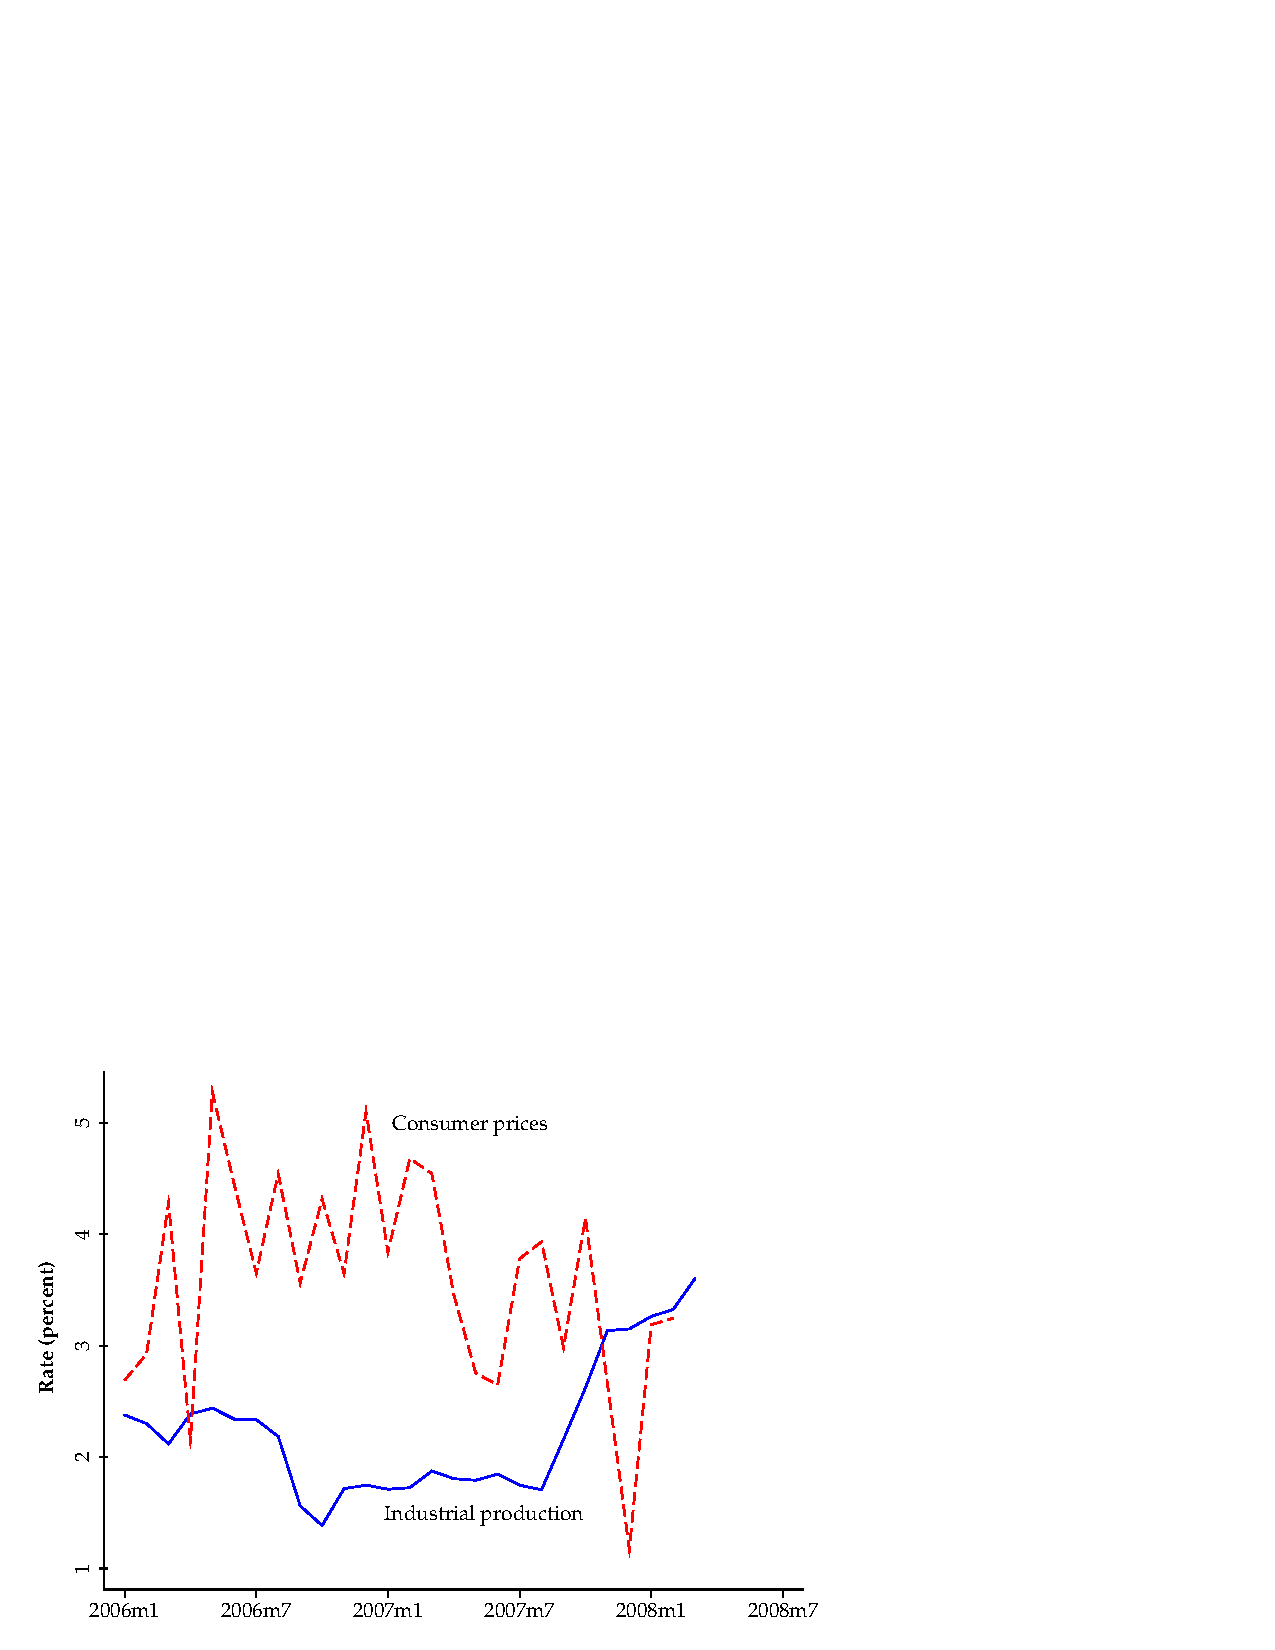
\includegraphics[width=0.8\textwidth]{Figures/eu_asad.pdf}
%    \caption{Growth in prices and industrial production in the
%    Euro Zone.}
%    \label{fig:ez}
%\end{figure}
%
%\item aggregate supply (AS) \index{aggregate supply (AS)}
% and demand in the Euro Zone,
%May 2008.
%As the CFO of Heineken International, you are considering
%the likely evolution of interest rates in the Euro Zone.
%You quickly run through the following questions:
%%
%\begin{enumerate}
%
%\item Over the 2-year period as a whole,
%    what has happened to inflation and output?
%    See Figure \ref{fig:ez}.
%
%\item In the aggregate supply (AS) \index{aggregate supply (AS)}
% and demand framework,
%    do you think the movements in prices and output
%    you mentioned above suggest a shift in supply or demand?  Why?
%    In principle,
%    how should the European central bank \index{central bank} respond to such a shift?
%
%\item How do you think the European central bank \index{central bank} is
%likely to respond?
%How do you see short-term Euro Zone
%interest rates moving over the next 12 months? Why?
%
%\end{enumerate}
%
%
%%\begin{comment}
%Answer.
%\begin{enumerate}
%\item Inflation is up sharply, output is flat to down.
%
%\item The combination in (a) suggests a shift up/left in supply.
%Why?  Because output and inflation have moved in opposite directions.
%Since supply shocks should be accommodated/reinforced,
%the ECB should raise the short-term interest rate.
%
%\item The ECB's primary mission is stable prices,
%so you should see an increase in interest rates.
%This could also be expressed in terms of a Taylor rule,
%possibly with a larger coefficient on inflation
%than output growth.
%\end{enumerate}
\end{enumerate}
%\setlength{\leftmargini}{\oldleftmargini}


\section*{If you're looking for more}

The measurement of potential output has generated some interesting debate.
The bottom line, in our view, is that there's usually some question
where the   long-run aggregate supply \index{aggregate supply (AS)!long-run aggregate supply}\index{aggregate supply (AS)}
 curve is. Here is a range of opinion on the subject:
%
\begin{itemize}
\item The Congressional Budget Office (CBO) reviews a number of approaches.
Search: ``cbo potential output.''
%\url{http://www.cbo.gov/sites/default/files/cbofiles/ftpdocs/51xx/doc5191/03-16-gdp.pdf}.

\item Former Fed Governor Frederic Mishkin's speech,
``Estimating potential output,'' is another good overview.
Search:  ``mishkin potential output.''

\item The Kansas City Fed's 2005 Jackson Hole Symposium has
an interesting exchange between Robert Hall and Greg Mankiw.
Hall argues that potential output may very well not be smooth,
which would contradict most measures of it.
As a practical matter, this would change our view of monetary policy dramatically
since many of the movements we see in GDP would be the result of the invisible hand
and, therefore, not something for policymakers to resist.
Mankiw says maybe, maybe not.
Search:  ``Jackson Hole Symposium 2005.''
%\centerline{\url{http://www.kc.frb.org/publications/research/escp/escp-2005.cfm}}
\end{itemize}

\needspace{18\baselineskip}
\section*{Symbols and data used in this chapter}

\begin{table}[H]
\centering
\caption{Symbol table.}
\begin{tabular*}{0.7\textwidth}{l@{\extracolsep{\fill}}l}
\toprule
Symbol & Definition\\
\midrule
$Y$    &Real output (=real GDP)\\
$Y^*$    &Equilibrium (or potential) output\\
${Y^{*}}'$    &New equilibrium (or potential) output\\
AS    &Short-run aggregate supply \\
AS$^*$    &  Long-run aggregate supply\\
AD    &Aggregate demand\\
AD$'$    &Aggregate demand after a shock\\
AS$'$    &Aggregate supply  after a shock\\
\bottomrule
\end{tabular*}
\end{table}

\begin{table}[h]
\centering
\caption{Data table.}
\begin{tabular*}{0.7\textwidth}{l@{\extracolsep{\fill}}l}
\toprule
Variable & Source\\
\midrule
NBER recession indicator    &USRECM\\
CBO real potential GDP        &GDPPOT\\
Oil Price (WTI)                &OILPRICE\\
\bottomrule
\addlinespace
\end{tabular*}
\begin{minipage}{0.7\textwidth}
\footnotesize{To retrieve the data online, add the identifier from the source column to \url{http://research.stlouisfed.org/fred2/series/}.
For example, to retrieve oil prices, point your browser to
\url{http://research.stlouisfed.org/fred2/series/OILPRICE}}
\end{minipage}
\end{table}

\chapter{Money and Interest Rates}\label{chp:mpir}
\hypertarget{monpol}{}

%No extra line here.
\textbf{Tools:} Open market operations; central bank balance sheet; Taylor rule.

\textbf{Key Words:} Real interest rate; nominal interest rate; expected inflation; real money balances; inflation targeting; interest-rate rules; rules vs. discretion; zero lower bound; quantitative easing; credit easing; policy duration commitment.

\textbf{Big Ideas:}
%\vspace{-0.1in}
\begin{itemize}
    \item In conventional practice, central banks use open market operations to manage interest rates. These policy actions are equivalent to managing the money supply directly.
    \item The Taylor rule provides a guide to how central banks manage their target interest rates in response to data on inflation and (real) GDP growth.
    \item When interest rates are at or near zero, a central bank can resort to unconventional monetary policy, including quantitative easing, credit easing, and policy-duration commitments. These policies have been in widespread use since 2008.
\end{itemize}

\rule{\textwidth}{1pt}

Where do interest rates come from?\index{interest rate|(textbf}
We doubt this was your first question when you were growing up,
but you probably have an opinion about it now.
Most people say they're set by the Fed --- or the appropriate central bank if you're in another country.
There's some truth to that, but it can't be that simple. We had interest rates before the Fed was established,
and, if anything, they varied more then than now.
It's probably better to say that the Fed ``manages'' interest
rates --- that is they vary the supply of money to set the market interest rate
they think is appropriate, consistent with market conditions. Market
interest rates reflect, after all, the behavior of private
borrowers and lenders, as well as the Fed.

We outline how this works, starting with
a review of interest rates (there are lots of them)
and moving on to monetary policy as practiced in most
developed countries these days.
Along the way, we show how you would expect new information
about inflation\index{inflation} or economic growth to affect interest rates.

\begin{comment}
*** predictability critical...

Commitment devices...
Gold and commodity money?  fixed exch rate?
Independent central bank \index{central bank}?
\end{comment}


\section{Interest rates}

Here's a quick review of interest rates:  real and nominal,
short and long, risk-free and risky.

\textbf{Real and nominal.} It may not strike you at first, but interest rates have units.
The  interest rates
 we're used to are reported in currency units:
A one-period bond \index{bond} pays currency later in return for
currency now.
That's one of the reasons why interest rates differ around the world:
If countries have different currencies, their interest rates
are measured in different units.
Since they're measured in currency units, we refer to them
as nominal interest rates,
just as GDP measured in currency units is referred to
as nominal GDP.\index{interest rate!nominal}

It's traditional, as we saw in Chapter \ref{chp:mpin},
to decompose a nominal interest rate
 $i$
into a real interest rate\index{interest rate!real}
 $r$
and expected inflation $\pi^e$:
%
\begin{eqnarray}
    i &=& r + \pi^e .
    \label{eq:fisher}%
\end{eqnarray}
%
The real interest rate
``corrects'' the nominal rate for the loss of purchasing power
reflected in the inflation\index{inflation} rate.
In words:  A nominal interest rate of five percent
delivers greater purchasing power in a year
if the inflation rate is two percent than if it is five percent.

\textbf{Short and long.}
bonds \index{bond} differ, of course, by maturity:  that's
the idea behind the ``term structure of interest rates\index{interest rate!term structure of interest rates},''
a popular finance topic.
If we consider a zero-coupon bond \index{bond} of maturity $m$ years,
the price and (nominal) interest rate or yield \index{bond!bond yield}
 are related by
\[
    q_m \;\;=\;\;  100/(1+i_m)^m .
\]
The interest rate has been annualized --- that's what the exponent does --- but it applies
to a bond \index{bond} whose maturity can be something besides one year.


Interest rates on long bonds\index{bond} often differ from those on short bonds. \index{bond}
Long rates are higher than short rates, on average,
but not always.
We commonly attribute the difference to two factors.
The first is expected differences in interest rates over the life of the bond\index{bond}:
If we expect short-term interest rates to rise over the life
of the bond\index{bond}, then its interest rate should be higher
as a result.
The second is risk.
Long bonds \index{bond} have greater exposure to the risk of changing interest rates.
Their price and yield \index{bond!bond yield}, therefore, incorporate adjustments for this risk.
We can express this in an equation as \index{risk premium}

\[
    i_m \;\;=\;\; \mbox{Expected Future Short Rates}
                  +  \mbox{Risk Premium} .
\]

Long-term interest rates have a similar distinction between real and nominal. \index{interest rate!long-term}
The equation is the same with the appropriate maturities noted:
\[
    i_m \;\;=\;\; r_m + \pi_m^e .
\]
For example, the expected inflation rate in this case is the one
that applies to the period from now until $m$ years from now.

\textbf{Credit risk. \index{credit risk}} There's another source of risk
that comes up later in the course:
the possibility that the borrower defaults.
We tend to ignore that in the US Treasury market, although
credit default swaps now price in some such risk.
With bonds \index{bond} issued by banks, corporations, and foreign ``sovereigns''
(governments), the risk can be substantial.
We might see, for example, that interest rates on Argentine or Greek
government bonds \index{bond} are several hundred basis points above US Treasuries
of similar maturity.
(A basis point is one hundredth of a percent.\index{basis point})


\section{Changing the money supply (review) \index{monetary policy}}

We'll come back to interest rates shortly.
But before we do, we consider monetary policy,
which plays a central role in their short-term movements.
central banks \index{central bank} control the quantity of currency
in circulation (money, for our purposes).
We show here how that works,
then move on in later sections to describe
how they use their control over money to influence interest rates.
Our analysis of the central bank's \index{central bank} control
of the money supply involves the balance sheets of the treasury,
the central bank\index{central bank}, and individuals and firms.
You've seen this before, but it's
important enough to run through again.
We'll see it again when we look at fixed exchange rates.\index{exchange rate regime!fixed exchange rate}


Day-to-day monetary policy in most countries consists of what we term
{\it open-market operations\index{monetary policy!open-market operation}\/}:
purchases or sales by the central bank \index{central bank} of government securities (bonds \index{bond}).
At any point in time, the treasury's balance sheet \index{Treasury!balance sheet} \index{Treasury}
 looks something like this:
%
\begin{center}
\begin{tabular}{lr|lr}
\multicolumn{4}{l}{Treasury} \\
\hline
Assets\phantom{ities} & \phantom{100}&  Liabilities \\
\hline
\phantom{bonds} & \phantom{200} & bonds \index{bond} & 200
\end{tabular}
\end{center}
%
The central bank's \index{central bank} looks like this:
%
\begin{center}
\begin{tabular}{lr|lr}
\multicolumn{4}{l}{Central bank \index{central bank}} \\
\hline
Assets\phantom{ities} &\phantom{100}&  Liabilities \\
\hline
bonds \index{bond} &  100 & Money & 100
\end{tabular}
\end{center}
%
And the private sector's looks like this:
%
\begin{center}
\begin{tabular}{lr|lr}
\multicolumn{4}{l}{Private sector} \\
\hline
Assets\phantom{ities}  &&  Liabilities \\
\hline
Money &  100  &  \phantom{Money} & \phantom{100} \\
bonds \index{bond} &  100  \\
Other &  500
\end{tabular}
\end{center}
%
If it seems strange to treat money as a liability of the
central bank \index{central bank}, think of it as a bond \index{bond} with the unusual
feature that its nominal interest rate is zero.\index{interest rate!nominal|(}
That's what it is, which makes it a good deal for the borrower.


An open-market purchase of bonds \index{bond} results in an increase
in bonds \index{bond} held by the central bank \index{central bank} and an equal increase in its
monetary liability.
The private sector does the opposite;  it sells bonds \index{bond} to
the central bank\index{central bank}, reducing its holdings of bonds \index{bond} and
increasing its holdings of money (currency).
For example, a central bank \index{central bank} purchase of 20 dollars worth of bonds \index{bond} would change
the balance sheets to
%
\begin{center}
\begin{tabular}{lr|lr}
\multicolumn{4}{l}{Central bank } \\
\hline
Assets\phantom{ities}  &&  Liabilities \\
\hline
bonds \index{bond} &  120 & Money & 120
\end{tabular}
\end{center}
%
%and
%
\begin{center}
\begin{tabular}{lr|lr}
\multicolumn{4}{l}{Private sector} \\
\hline
Assets\phantom{ities}  &&  Liabilities & \phantom{100} \\
\hline
Money &  120  &  \phantom{Money} & \phantom{100} \\
bonds  &  \phantom{1}80 \\
Other &  500
\end{tabular}
\end{center}
%
Note that this doesn't change anyone's net worth;
it's a portfolio shift, which changes only the composition
of assets and liabilities. \index{monetary policy!open-market operation}
The result is an increase in the amount of money in private hands
since the private sector (the other side of this transaction)
has reduced its holdings of government bonds \index{bond} and increased its holdings of money.
Similarly, an open-market sale of bonds \index{bond} would reduce the amount of money in
private hands.


\section{Managing the interest rate}

Typically, we describe monetary policy in terms of
managing the short-term interest rate,
which is different from what we've described before
(namely, controlling the money supply).
How does managing the money supply relate to managing the short-term interest rate?
Let's work through the impact of a change in the supply of money in a simple model.

This is essentially a supply and demand exercise,
and the first step is to describe the demand for money.
Consider a modified version of the quantity theory:
\begin{eqnarray}
    M_t/P_t  &=&  Y_t / V(i_t).
    \label{eq:md}
\end{eqnarray}
Here (as before), $M$ is the supply of money (think currency),
$P$ is the price level (think price index),
$Y$ is real output (real GDP),\index{gross domestic product (GDP)!real GDP}
and $V(i_t)$ is velocity.
We refer to the $M/P$ as {\it real balances\/}:  the real value of money
issued by the central bank \index{central bank} and held by the public.

Our key innovation here is allow velocity to increase with the nominal interest rate.
When the nominal interest rate is high, we will assume that velocity is high,
and vice versa.
As a result, real money balances ($M/P$) decline when the nominal interest rate rises.
We noted the same thing in Chapter \ref{chp:mpin},
where we noted that at high inflation\index{inflation} rates people did anything they could to avoid money,
thereby raising its velocity.
They same rationale applies in less extreme settings:
when the nominal interest rate is high,
people shift their portfolios from non-interest-bearing money to interest-bearing assets.


In Figure \ref{fig:ms=md} we plot supply and demand curves for money with the
nominal interest rate $i$ on the y-axis and real money balances $M/P$ on the x-axis.
The downward-sloping line is the demand for real balances.
Its slope illustrates the relationship between real balances and the nominal interest rate:
As the nominal interest rate rises, the quantity of money demanded falls.
The vertical line is the supply of real balances.
At a given value of $P$, this line is vertical
because supply is determined by the central bank. \index{central bank}

We now have a model of the supply and demand for real balances
and can explore the relation between the supply of money and the nominal interest rate.\index{interest rate!nominal|)}

%%%%%%%%%%%%%%%%%%%%%%%%%%%%%%%%%%%%%%%%%%%%%%%%%%%%%%%%%%%%%%%%%%%%%%%%%%%%
%  Supply and demand diagram
\begin{figure}[h!]
\caption{Supply and demand for money.}
\label{fig:ms=md}
%
\centering
\setlength{\unitlength}{0.075em}
\begin{picture}(250,200)(0,0)
%\footnotesize
\thicklines

% horizontal axis
\put(-30,0){\vector(1,0){300}}
\put(255,-16){$M/P$}

% vertical axis
\put(0,-20){\vector(0,1){200}}
\put(-15,155){$i$}

% demand
\put(25,165){\line(4,-3){200}}\put(230,10){$Y/V$ (demand)}

% supply
\put(120,0){\line(0,1){170}} \put(106,176){$M/P$}
\put(160,0){\line(0,1){170}} \put(146,176){$M'/P$ (supply)}

% equilibrium labels
\put(108,80){\footnotesize A}
\put(148,53){\footnotesize B}
% dotted lines
%\qbezier[31]{(133,0)(133,46)(133,92)}
%\qbezier[45]{(0,92)(67,92)(133,92)}
%\qbezier[45]{(0,72)(67,72)(133,72)}

\end{picture}
\begin{minipage}{0.7\textwidth}
\vspace{0.4in}
{\footnotesize The very short-run impact of an increase in the money supply
is a shift right in the vertical supply curve ($M/P$)
and a movement down the demand curve ($Y/V$) from A to B.}
\end{minipage}
\end{figure}
%%%%%%%%%%%%%%%%%%%%%%%%%%%%%%%%%%%%%%%%%%%%%%%%%%%%%%%%%%%%%%%%%%%%%%%%%%%%

\textbf{What happens if the central bank \index{central bank} increases the supply of money $\mathbf{M}$?} There are two outcomes, one in the long run and one in the short run.
In the long run, the price level increases proportionally with the money supply, and the supply curve stays in the same place and nothing changes. That's the logic of the quantity theory taken literally: Any increase in money (in the long run) results in an increase in prices.

In the short run, the results differ. In the short run, we might guess that production plans won't change ($Y$ is fixed), and we generally think that prices won't change either ($P$ is fixed).
Then the money-supply curve shifts out and the interest rate falls.
In the figure, we move from point $A$ to point $B$.
In words: By increasing the supply of money, the central bank \index{central bank} drives down the interest rate.

The key point here is that we can think of changes in the interest
rate as reflecting changes in the money supply.
Put this way, there's little difference between changing the money supply
and changing the interest rate.

One last thought:  Context matters here.
If the context is relatively stable prices, changes in the
money supply affect the interest rate as described.
But if an increase in the money supply is interpreted as a sign
that the central bank \index{central bank} is abandoning price stability,
then we could see an increase in the supply of money
raise the interest rate rather than lower it.
% ?? more
That's why you hear central bankers \index{central bank} talk about ``anchoring expectations''
and ``maintaining credibility'' for stable prices.
More on that shortly.

\section{Goals of monetary policy\index{monetary policy!goals}}

If the tools of monetary policy are the money supply and the short-term
interest rate, what is the goal?
Should central banks \index{central bank} focus
on inflation, growth, or some combination?
This, in turn, raises the question of what they're capable of doing.
There is clear evidence that monetary policy affects inflation,
at least over periods of several years.
Persistent high inflation\index{inflation} is invariably associated with
high rates of money growth.
There is also clear evidence that
countries with high and variable inflation rates have poor
macroeconomic performance,
although the cause and effect are less clear. Is high inflation the cause of poor economic performance,
or the result?

With these facts in mind, most countries charge their central
banks with producing stable and predictable prices. In practice,
this is typically understood to mean a stable inflation rate of
about 2 percent a year.
Many advanced economies have also made their
central banks \index{central bank} independent --- in the sense that they can set their
policy instrument (usually an interest rate) without being overridden
by a legislature or a government for short-run political reasons.
(Argentina did this, too, but it didn't last very long.)

Why have so many countries granted their central banks \index{central bank} such
 ``instrument independence?" One reason is that it helps overcome
 a classic  \hyperref[sec:time_cons]{time-consistency problem}.\index{time consistency}
If people expect a government
with a short time horizon to set monetary policy, they would expect it to stimulate
the economy now even if that spells high inflation later.
%Professor Kenneth
%Rogoff (former IMF chief economist) has shown that
But if countries appoint conservative central bankers\index{central bank},
they can --- in theory, at least --- reduce inflation without loss of output.
When an independent monetary authority can commit credibly to keep
inflation\index{inflation} low, it lowers inflation expectations today and improves
both inflation and output performance.

In the US, the Federal Reserve Act asks the Fed ``to promote the
goals of maximum employment, stable prices, and moderate long-term
interest rates."\index{interest rate!long-term}
This is, to be sure, the usual political mush --- the Fed should
accomplish ``all of the above.''
The term ``maximum employment'' is interpreted to mean
that the Fed should act to reduce the magnitude and duration of
fluctuations in output and employment.
What role does monetary policy play in these fluctuations?
In the long run, expert opinion is that the impact is close to zero;
the long-term growth rate of the economy depends on its productivity and institutions,
not on its monetary policy.
But in the short run, expansionary monetary policy
(high money growth, low interest rate)
probably has a modest positive effect on
employment and output.
The connection is fragile, in the sense that too much monetary expansion seems to lead not to higher
output but to high inflation\index{inflation}, higher interest rates,
and, perhaps, lower output.
Most experts suggest, therefore,
that central banks \index{central bank} (including the Fed) should emphasize
price stability and give secondary importance to output and
employment.


One of the arguments in favor of price stability is that
our attempts to do more
have been notably unsuccessful.
Ben Bernanke\index{Bernanke, Ben} put it this way in a 2003
\href{http://www.federalreserve.gov/boarddocs/Speeches/2003/20030203/default.htm}
{speech} at NYU (``Constrained discretion''):
%
\begin{quote}
The early 1960s [were] a period of what now appears to have been
substantial over-optimism about the ability of [monetary]
policymakers to `fine-tune' the economy. Contrary to the expectation
of that era's economists and policymakers, the subsequent two
decades were characterized not by an efficiently managed, smoothly
running economic machine but by high and variable inflation and an
unstable real economy, culminating in the deep 1981-82 recession.
Although a number of factors contributed to the poor economic
performance of this period, I think most economists would agree that
the deficiencies of ... monetary policy --- including over-optimism
about the ability of policy to fine-tune the economy ... played
a central role.
\end{quote}
%
Another way to put this: Economists should be humble about what we can
accomplish.
(And to paraphrase Winston Churchill, we have a lot to be humble about!)


The focus on price stability is often expressed as
a desire for predictability.
Firms, investors, and workers all need to have a clear picture
of future inflation --- hence, future monetary policy --- since the consequences of current decisions depend on it.
Built into this statement is a belief that many such decisions ---
prices of bonds\index{bond}, wages and salaries, long-term supply contracts ---
are expressed in units of currency, whose future value depends on policy.
Therefore, it's helpful for policy to be predictable, so that these
decisions can be made according to their economic merits
rather than on guesses of future policy.
As Bernanke\index{Bernanke, Ben}
 suggests, the unpredictability of policy in the 1970s was a factor in
the poor macroeconomic performance of that decade.
Big inflations\index{inflation} are an extreme example,
in which even day-to-day price changes are not only large, they're wildly uncertain.
In such conditions, capital markets typically either disappear
or shift to another currency.

With these ideas in mind,
many central banks \index{central bank} now follow procedures that focus on price
stability (so that people can make long-term decisions)
and transparency
(so that their actions are well understood).
In the industrial world, targeting inflation over the medium term (say, over
several years) has become common. The Federal Reserve announced
a quantitative inflation goal \index{monetary policy!inflation targeting}
 \index{monetary policy!inflation target}
 (of 2 percent) for the first time in 2012.
In developing countries, fixed exchange rates are a common device
in which a currency is tied to one that is thought to be more predictable.
Most commonly, there has been a move toward interest-rate rules
that connect (at least approximately)
interest rates set by central banks \index{central bank} with inflation and (possibly) output.


\begin{comment}
For those who are left, I also want to show how future policy affects
the market reaction to current policy,
which leads us back to the conclusion
that monetary policy should be reasonably predictable.

Now to the second issues:  the impact of future policy on the present.
Even in this relatively simple setting, you can get a sense
of the challenges of thinking through the dynamic effects of monetary policy.
The nominal interest rate, for example, is the real interest rate plus
expected inflation:
\[
    i_t \;=\; r_t + \pi_{t+1}.
\]
From this, you can see that the impact of any policy change
depends in part on its impact on expected inflation.
If the impact is zero, you get what we had above.
But if an increase in the current money supply leads
people to expect higher inflation
(remember:  the long-run impact is a rise in the price level),
then this could offset the impact on the interest rate.
People will demand higher interest rates to compensate them for
higher inflation.
How will people make these calculations?
They need to know what policies are likely to follow the current change in
the money supply.
Will the money supply stay at its new level indefinitely?
Will the increase be offset in a month or two?
None of these issues show up in the figure,
but they're central to the impact of the policy.

%\begin{comment}
The same issues show up when we take a closer look at the AS/AD model \index{AS/AD model}
.
You might think from our earlier analysis that we can change
output as we like simply by shifting the aggregate demand (AD) \index{aggregate demand (AD)}
 curve around.
For example, if we increase the money supply,
that shifts AD to the right, increasing output and prices.
The only question is how much inflation we're willing to tolerate
to get higher output.
That's the Phillips curve tradeoff that many of you are familiar with:
high inflation or high unemployment (hence low output)?
In a dynamic theory, as in real life, it's not that easy.
Suppose the aggregate supply (AS) \index{aggregate supply (AS)}
 curve is based on sticky wages.
What wages will workers and firms set?
Generally they will need to take into account future monetary policy,
since it will have an impact on future inflation and hence
the purchasing power of any nominal wage rate.
That tells us, in essence, that we can't determine the
impact of current policy until we've said what future policy will be.
It's a central feature of a dynamic world:
that you can't separate the present from expectations about the future.
The same is true of economic activity more generally,
which is why institutions are so important:
they give us some assurance that future policies will not
be wildly different from the present.
%\end{comment}

The bottom line:  one goal of modern central bankers \index{central bank} is
to make clear to market participants how they make decisions
about monetary policy ---  not just current decisions but future
ones as well.
Anything less could lead to the chaos and poor performance
we saw in the 1970s.
That leads us to consider policy rules...
\end{comment}


\section{The Taylor rule:\index{monetary policy!Taylor rule}
 the bond \index{bond} trader's guide \index{monetary policy!interest-rate rules}}

One way to make monetary policy predictable and transparent
is to follow a rule.  The rule tells us how policy will be set,
at least approximately, both now and in the future,
which makes policy more predictable
to market participants, including bond \index{bond} traders.

As we saw in previous chapters, concerns about \hyperref[sec:time_cons]{time consistency}
tend to favor rules over discretion in setting economic policy.\index{time consistency}
In the case of monetary policy, a well-designed rule can help anchor
inflation expectations and stabilize economic activity.
It does so by limiting the scope for future policymakers to renege on
their commitment to low inflation\index{inflation} in return for politically popular short-term output gains.

The rules vs. discretion debate has a long history, \index{monetary policy!rules vs discretion}
and a number of monetary policy have been proposed over the years.
One of the most famous is Milton Friedman's $k$-percent rule,
which called for the central bank \index{central bank} to increase the supply of  money at a constant rate of $k$-percent.
Subsequent research suggests that a ``feedback rule'' which responds to economic conditions will be more effective in stabilizing inflation and economic growth over business cycles\index{business cycle}.
In addition, most research --- and virtually all central bank \index{central bank} practice ---
focuses on rules for setting the policy interest rate, rather than the supply of money.

Of these interest-rate feedback rules, the most famous and widely used is the {\it Taylor rule\/}.
John Taylor \index{Taylor, John}
 %, a Stanford economist and former treasury official,
suggested in 1993 that an interest-rate rule would provide a
relatively simple summary of monetary policy in many countries.
It's a guideline really, not a rule, but it nevertheless goes
by the name ``Taylor rule.''
It consists of the following equation:
\begin{equation}
    i_t  \;\;=\;\;  r^* + \pi_t + a_1 (\pi_t - \pi^*)
            + a_2 (y_t - y_t^* )   ,
    \label{eq:taylorrule}
\end{equation}
where $i_t$ is the short-term nominal interest rate;
$r^*$ is a ``normal'' or long-term average real interest rate;
$\pi_t  $ is the inflation\index{inflation} rate;
$\pi^*$ is the target inflation rate;
$y_t$ is (the logarithm of) real output;
and $y_t^*$ is the ``normal'' (sometimes called ``potential") level of output (also in logarithms).
The parameters $a_1,\ a_2$ indicate the sensitivity of the interest rate to
inflation and output.


Let's walk through equation (\ref{eq:taylorrule}) piece by piece,
as applied in the US:
%
\begin{itemize}
\item \textbf{Nominal interest rate $i$.}
Standard practice in the US is to use the ``fed funds rate.''
In the US, commercial banks and other ``depository institutions'' have accounts (deposits) at the Federal Reserve that are referred to as fed funds.  They trade these deposits among themselves in an
overnight fed funds market.
The Fed currently indicates its policy stance by setting an explicit
target for the interest rate on these trades
and performs open-market operations
to bring the market rate close to the target.
This rate anchors the very short end of the yield \index{bond!bond yield}
 curve.\index{interest rate!nominal}

\item \textbf{Normal real interest rate $r^*$.}  Experience suggests that the real fed funds rate (nominal rate minus inflation) has averaged about two percent over the last two decades, but it moves around over time, both over long periods of time
(real interest rates were unusually high in the 1980s
and low in the 2000s)
and over the business cycle.\index{interest rate!real}
Most people simply set $r^* = 2\%$.
The first component of the target fed funds rate is,
thus, the target real rate (two percent) plus the current inflation\index{inflation} rate, thus giving us a nominal interest rate target.

\item \textbf{Inflation deviation $(\pi - \pi^*)$.}  The next term is a reaction to the difference between current inflation ($\pi$)
    and the target ($\pi^*$).
If the target is two percent and actual inflation\index{inflation} is three percent, then we
increase the nominal fed funds rate by $a_1$ percent.
Typically $a_1 > 0$, meaning that we increase the
interest rate in response to above-target inflation.
Why?  Because higher interest rates are associated with slower money growth
and, therefore, (eventually) lower inflation.
Larger values of $a_1$ indicate more aggressive reactions to inflation.
Since inflation enters equation (\ref{eq:taylorrule}) both directly \emph{and} as part of this term,
any increase in inflation leads to a greater increase in the nominal
interest rate.
This ``overreaction'' is intended to stabilize the inflation rate.

\item \textbf{Output deviation\index{output gap}
 $( y - y^*)$.}
The final term is a reaction of the interest rate
to deviations of output from its normal or potential level.
Some people use a smooth trend for $y^*$
or a measure of potential output.
(You may recall the discussion of Chapter \ref{chp:pasad}.)
If we think of the world as the AS/AD model\index{AS/AD model}, then potential output is
what the economy would generate if wages and prices weren't sticky --- whatever that is!
The Fed's goal, in this case,
is to offset the impact of those frictions on output.
The practical difficulty is distinguishing
increases in $y$ from increases in $y^*$.
One approach is to use the difference in the year-on-year
growth rate from its mean.
This is easier to measure,
but has the same issue:  it's not obvious that our measure
(the mean growth rate) is the same as the long-run equilibrium.


\item \textbf{Parameters $(a_1, \ a_2)$.}
Taylor suggested $a_1 = a_2 = 1/2$,
giving equal weight to inflation and output deviations.
Some recent studies of actual central bank \index{central bank} behavior find larger values of $a_1$
and smaller values of $a_2$ --- say
$a_1 = 0.75$ and $a_2 = 0.25$.
By some interpretations, the European central bank \index{central bank} (ECB)
places greater weight than the Fed on inflation
and less weight on output.
\end{itemize}

That's the rule.
The bond \index{bond} traders' perspective is that it's a reasonable guide to how
short-term interest rates respond to data releases,
as bond \index{bond} traders respond to how they see monetary policy reacting
to new information about economic conditions.
If a high inflation\index{inflation} number comes out, the interest rate goes up.
Why?  Because they know that this will lead the central bank \index{central bank} to raise
the short-term interest rate.
Even if the Fed doesn't respond immediately,
long yields \index{bond!bond yield}
 may rise in anticipation of future interest-rate changes.
Ditto a high output number: Short- and long-term interest rates rise.
The timing may differ somewhat from the rule,
but its overall impact is generally similar.


There are several issues you run across in practice.
One is that the Fed (or other central banks \index{central bank}) may deviate from
the rule, perhaps on principle, perhaps because of special circumstances.
Despite its widespread use, no central bank \index{central bank} is on record
saying that it follows such a rule.
Another is the difficulty in determining $y^*$.
If output goes up, do we decide that the economy is overheating
and raise the interest rate?
Or do we decide that productivity has gone up,
increasing the growth of the economy and $y^*$?
That's exactly the issue that the Fed faced in the late 1990s.
Some felt that the rule dictated higher interest rates,
but Greenspan argued that $y^*$ had gone up because
productivity growth had accelerated.
This goes back to our distinction between
supply shocks and demand shocks. \index{supply shocks}
In the AS/AD framework,
demand shocks should generally be resisted,
but supply shocks should be accommodated/acquiesced to. Yet another issue is that the
normal real interest rate\index{interest rate!real} $r^*$ may change over time (for example, it might be high
when productivity growth is high, reflecting the marginal productivity\index{capital!marginal product of}  of capital).

Despite these open issues, the Taylor rule has been a reasonably
reliable guide to policy
and a useful indication of how bond \index{bond} markets respond to announcements
of macroeconomic activity.


\begin{comment}
\section{FOMC statements}

The Federal Open Market Committee (FOMC), the monetary policy arm
of the Federal Reserve System,
now issues short statements immediately following each of their meetings.
The statements are important both for their announcement
of the target fed funds rate ($i$ in the Taylor rule)
and for their analysis of the economy and what future policy may bring.
Here's the complete statement from January 31, 2007 [numbers added]:
%
\begin{quote}
1. The Federal Open Market Committee decided today to keep its
target for the federal funds rate at 5-1/4 percent.

2. Recent indicators have suggested somewhat firmer  economic
growth, and some tentative signs of stabilization have appeared in
the housing market. Overall, the economy seems likely to expand at a
moderate pace over coming quarters.

3. Readings on core inflation have improved modestly  in recent
months, and inflation pressures seem likely to moderate over time.
However, the high level of resource utilization has the potential to
sustain inflation pressures.

4. The Committee judges that some inflation risks remain.  The
extent and timing of any additional firming that may be needed to
address these risks will depend on the evolution of the outlook for
both inflation and economic growth, as implied by incoming
information.
\end{quote}
See
\href{http://www.federalreserve.gov/boarddocs/press/monetary/2007/20070131/default.htm}
{link}.

%
Let's go through it line by line.
Line 1 says that they have decided not to change the fed funds rate.
That speaks for itself.  But why?
Line 2 says that the housing market, a current concern,
is thought to be stabilizing.
This is more positive than the previous statement that
the housing market exhibited ``substantial cooling.''
The last sentence suggests that the Fed now sees output growth as stronger
than in the previous statement,
where a similar statement included the qualification ``on balance.''
The interpretation in both cases is that there is less reason to suspect that the Fed will respond by reducing rates ---
roughly speaking, the output component of the Taylor rule.
Line 3 says that inflation numbers have come down, which on its own
suggests less reason to raise interest rates --- the Taylor rule again.
Line 4 says that any change in policy will depend on
how inflation and output growth evolve in the coming months.
Taken together, they give us a picture of what future policy
is likely to be.
\end{comment}


\section{Deflation\index{deflation}}

Some people are concerned with the possibility of deflation:
a decline in prices or negative inflation.
There are two good reasons for this.
One is a couple of well-documented episodes in which deflation was associated
with poor economic performance:
the US in the Great Depression and Japan in the 1990s.
The other reason is that deflation raises the real value of debt,
which makes it more difficult for borrowers to repay them.
Modest temporary deflation is unlikely to have much effect,
but large sustained unexpected deflation, such as the US experienced in the early 1930s,
likely has an adverse effect on the economy.

Whether that's the case or not, the issue comes up regularly in policy discussions.
Examples include Japan during the 1990s, the US during the financial crisis,
and Europe today.


\section{Quantitative easing\index{monetary policy!quantitative easing}, credit easing, and signaling}

If the short-term interest rate falls to zero, or close to it,
is the central bank \index{central bank} powerless?
This issue came up in Japan in the 1990s and
much of the developed world after 2008.
The answer is no, but let's review the logic --- and the collection of acronyms that go along it.\index{interest rate!nominal}

The so-called {\it zero lower bound\index{monetary policy!zero lower bound}\/} (ZLB) is a practical
limit on how low nominal interest rates can go.
Why can't they go lower?
Because currency guarantees a nominal interest rate of zero,
so there's no reason to accept anything lower.
Transaction costs and regulations that give preference
to short-term government securities have let interest rates
go a little below zero, but, as a practical matter, that's the limit.

If you follow (say) a Taylor rule and it indicates a negative interest rate,
what do you do?
Your first guess might be that you're stuck:  zero is it.
But remember:  You can always increase the money supply,
even if it doesn't lead to a fall in the nominal interest rate.
This change in the quantity of money is generally referred to as
{\it   quantitative easing\index{monetary policy!quantitative easing} \/} (QE).
For those of us who grew up thinking about monetary policy in
terms of the supply of money,
this has a back-to-the-future ring to it:
Isn't that how we used to talk?
The key is the new terminology,
which makes an old idea sound modern.
That marketing lesson apparently works as well in economics
as with consumer products.

In contrast to QE, which increases the size of the central bank's \index{central bank}
balance sheet, \index{monetary policy!credit easing}
{\it credit easing\/} (CE) shifts the composition of the balance sheet
from default-free assets toward assets with credit (or other kinds of) risk.
A classic example of CE is for the central bank \index{central bank} to sell Treasury debt
and buy mortgage-backed securities of the same maturity. Another example
is to exchange short-term assets for long-term assets (as in the Fed's
so-called Operation Twist).
Only the mix of assets has changed.
CE is thought to lower the cost and increase the supply of credit,
particularly when private markets are illiquid.

A different approach to policy at the ZLB is to commit future monetary
policy to keeping interest rates low.
If policymakers believe that inflation will stay below their target,
they can promise to keep their interest-rate target low
for an extended period.
The Fed has used {\it   policy duration commitments\/} \index{monetary policy!policy duration commitment} \index{monetary policy!forward guidance}
extensively since 2008, and occasionally before that.\index{interest rate|)}

\needspace{5\baselineskip}
\section*{Executive summary}

%\setlength{\leftmargini}{.5\oldleftmargini}
\begin{enumerate}
\item Most central banks use interest rates as their primary policy tool.

\item Theory and experience suggest that monetary policy
should emphasize price stability and predictability.

\item The Taylor rule is an approximate description of how
central banks set interest rates: They raise them in response to
increases in inflation\index{inflation} and reductions in output.

\item When interest rates hit zero, central banks can still implement
policy through quantitative easing, credit easing, or
commitments to future policy actions.\index{monetary policy!quantitative easing}
\end{enumerate}
%\setlength{\leftmargini}{\oldleftmargini}


%\begin{comment}
\section*{Review questions}

%\setlength{\leftmargini}{.5\oldleftmargini}
\begin{enumerate}
\item Real and nominal interest rates.
Consider the following information about inflation and US interest rates.
%\begin{enumerate}
%\item
If we ignore the difference between actual and expected inflation,
what was the real interest rate in each year presented in the table?
When was it highest?
%\end{enumerate}

\begin{center}
\begin{tabular}{lcc}
\toprule
        & Inflation Rate & One-Year yield \index{bond!bond yield}
 \\
\midrule
1980 & 8.75 & 12.05\\
1990 & 3.80 & 7.88\\
2000 & 2.15 & 6.11\\
2010 & 1.33 & 0.32\\
\bottomrule
\end{tabular}
\end{center}

Answer.  The real interest rates for the four dates
were 3.30, 4.08, 3.96, and --1.01.
The highest was 1990, but 2000 is close.
By far the lowest is 2010.

\item Money supply mechanics.  How does a central bank increase the money supply?
What is the likely effect on the short-term interest rate?

Answer.
It purchases government bonds from private agents,
giving them money in return.
An increase in the money supply reduces the short-term
interest rate.
The argument is that this increases liquidity in markets, reducing
the rate.
It depends on an overall environment of price stability.

\item Taylor rule in action.  If the inflation\index{inflation} rate rises,
how would a central bank following a Taylor rule respond?
Why?

Answer.  It would raise the interest rate.
Note that the interest rate rises by more than one-for-one
with inflation.

%\item In some countries, including the US,
%we can find $r$ directly from inflation-indexed
%bonds. \index{bond}  For these bonds \index{bond}, coupons and
%principal are adjusted for inflation: If prices increase 5 percent, then coupons
%and principal are increased 5 percent.
%Show that the yield \index{bond!bond yield}
% on such a bond is, in fact,
%the real interest rate $r$.
%
%Answer.  Apply the definitions.  What is the price now?
%What is the payment one year from now?

\item The Cleveland Fed has a beautiful
\href{http://www.clevelandfed.org/research/data/credit_easing/index.cfm}{chart}
that describes the asset side of the Fed's balance sheet since January 2007.
Search:  ``Cleveland fed credit easing.''
Which features of the chart represent quantitative easing (QE)?\index{monetary policy!quantitative easing}
Which represent credit easing (CE)?

Answer.
The large increase in the size of the Fed's asset positions in 2008
represents QE.
CE is less striking in its timing, but the increase in mortgage-backed
agency debt (brown) in 2009 is a good example.

\end{enumerate}
%\setlength{\leftmargini}{\oldleftmargini}


\section*{If you're looking for more}

For more on the art and science of monetary policy:
%
\begin{itemize}
\item Ben Bernanke's\index{Bernanke, Ben} speeches are typically clear and thoughtful.
See especially:
\begin{itemize}
\item
``\href{http://www.federalreserve.gov/boarddocs/speeches/2003/20030203/default.htm}
{Constrained discretion},'' February 2003.

\item ``\href{http://www.federalreserve.gov/boarddocs/Speeches/2004/20041202/default.htm}
{The Logic of monetary policy},'' December 2004.

\item
``\href{http://www.federalreserve.gov/BoardDocs/Speeches/2005/20050330/default.htm}
{Implementing Monetary Policy},''
March 2005.

\end{itemize}
\item The Cleveland Fed's
\href{http://www.clevelandfed.org/Research/Com2003/0703.pdf}
{\it Taylor rule guide\/}.
\end{itemize}


\section*{Symbols and data used in this chapter}

\begin{table}[H]
\centering
\caption{Symbol table.}
\begin{tabular*}{0.85\textwidth}{l@{\extracolsep{\fill}}l}
\toprule
Symbol & Definition\\
\midrule
$\pi^e$     &Expected Inflation\\
$i$                &Nominal interest rate\\
$r$                &Real interest rate ($= i- \pi^e$)\\
$q_m$             &Price of $m$-year bond  \\
$i_m$           &Nominal interest rate or yield
 on $m$-year bond \\
$\pi^e_m$       &Expected Inflation over $m$ years\\
$M$                &Money stock\\
$V(i)$             &Velocity of money as a function of interest rate $i$\\
$P$                &Price level\\
$Y$               &Real output or GDP\\
$Y^*$          &Equilibrium or potential real output\\
$r^*$          &Equilibrium real interest rate\\
$\pi^*$        &Target inflation rate\\
$y$               &Natural logarithm of $Y$ ($=ln[Y]$)\\
$y^*$          &Natural logarithm of $Y^*$\\
$a_1,a_2$      &Coefficients or weights in Taylor rule\\
%$\MB$           &Monetary base\\
%$M$              &Monetary aggregate (generic)\\
%M1           &Monetary aggregate ``M1''\\
%M2           &Monetary aggregate ``M2''\\
%$\CU$           &Currency\\
%$D$                &Deposits\\
%$RE$           &Reserves\\
%$\gamma$        &$\CU/D$\\
%$\rho$            &$RE/D$\\
\bottomrule
\end{tabular*}
\end{table}

\begin{table}[t]
\centering
\caption{Data table.}
\begin{tabular*}{0.90\textwidth}{l@{\extracolsep{\fill}}l}
\toprule
Variable & Source\\
\midrule
Federal funds rate    &FEDFUNDS\\
2yr Treasury yield
    &GS2\\
10yr Treasury yield
    &GS10\\
Moody�'s Baa corporate yield
    &BAA\\
BofA Merrill public sector     &BAMLEMPBPUBSICRPIEY\\
\phantom{mm}emerging market yield
 &\\
CBO real potential GDP    &GDPPOT\\
Real GDP    &GDPC1\\
consumer price index
    &CPIAUCSL\\
\bottomrule
\addlinespace
\end{tabular*}
\begin{minipage}{0.90\textwidth}
\footnotesize{To retrieve the data online, add the identifier from the source column to \url{http://research.stlouisfed.org/fred2/series/}.  For example, to retrieve the Federal funds rate, point your browser to \url{http://research.stlouisfed.org/fred2/series/FEDFUNDS}}
\end{minipage}
\end{table}

%%%%%%%%%%%%%%%%%%%%%%%%%%%%%%%%%This could cause problems later!%%%%%%%%%%%%%%%%%%%%%%%%%%%%%%%%%%%%%%%%
%%KR: the last table ends up on its own page, but vertically centered.  To force the table to the top, I've
%%added these two aweful lines below.
\vspace*{2em}
%%%%%%%%%%%%%%%%%%%%%%%%%%%%%%%%%%%%%%%%%%%%%%%%%%%%%%%%%%%%%%%%%%%%%%%%%%%%%%%%%%%%%%%%%%%%%%%%%%%%%%%%%


%
%THE FEDERAL RESERVE ACT LAYS OUT the goals of monetary policy. It specifies that, in conducting
%monetary policy, the Federal Reserve System and the Federal Open Market Committee should seek "to
%promote effectively the goals of maximum employment, stable prices, and moderate long-term
%interest rates."
%
%ECB
%
%The tasks of the ESCB and of the Eurosystem are laid down in the Treaty establishing the European
%Community. They are specified in the Statute of the European System of central banks \index{central bank} (ESCB) and of
%the European central bank \index{central bank} (ECB). The Statute is a protocol attached to the Treaty.
%
%The Treaty text refers to the 'ESCB' rather than to the 'Eurosystem'. It was drawn up on the
%premise that eventually all EU Member States will adopt the euro. Until then, the Eurosystem will
%carry out the tasks. Objectives "The primary objective of the ESCB shall be to maintain price
%stability".
%
%And: "without prejudice to the objective of price stability, the ESCB shall support the general
%economic policies in the Community with a view to contributing to the achievement of the
%objectives of the Community as laid down in Article 2." (Treaty article 105.1)
%
%The objectives of the Union (Article 2 of the Treaty on European Union) are a high level of
%employment and sustainable and non-inflationary growth.
%
%BOJ Act Chapter I General Provisions
%
%(Objectives) Article 1       The objective of the Bank of Japan, as the central bank \index{central bank} of Japan, is
%to issue banknotes and to carry out currency and monetary control. 2.      In addition to what is
%prescribed by the preceding Paragraph, the Bank's objective is to ensure smooth settlement of
%funds among banks and other financial institutions, thereby contributing to the maintenance of an
%orderly financial system.
%
%(The principle of currency and monetary control) Article 2       Currency and monetary control
%shall be aimed at, through the pursuit of price stability, contributing to the sound development
%of the national economy.
%
%(Respecting the autonomy of the Bank of Japan and ensuring transparency) Article 3       The Bank
%of Japan's autonomy regarding currency and monetary control shall be respected.



% Other topics
\part{Crises and Other Topics}
\chapter*{Crisis Overview}
\hypertarget{overview_other}{}

\rule{\textwidth}{1pt}

This outline covers key concepts from the third part of the course:
macroeconomic crises and other topics.
It is not exhaustive, but is meant to help you
(i)~anticipate what is coming and
(ii)~organize your thoughts later on.

\medskip
\textbf{\hyperref[chp:tax]{\underline{Taxes}} and \hyperref[chp:dbdf]{\underline{Government Debt and Deficits}}}

\textbf{Tools:} Welfare triangles; government budget constraint; debt dynamics.

\textbf{Key Words:} Tax wedge; deadweight loss; primary deficit/surplus.

\textbf{Big Ideas:}
\vspace{-0.1in}
\begin{itemize}
\item Tax systems should be (i) administratively simple and transparent and (ii) have a broad tax base.
\item Government spending must be paid for, either now through taxes, or in the
future by running primary surpluses.
\item Changes in the ratio of debt to GDP have three sources:
interest, growth, and primary deficits.
\end{itemize}


%\begin{comment}
\hyperref[chp:bop]{\textbf{\underline{International Capital Flows}}}

\textbf{Tools:} Balance of international payments; dynamics of net foreign assets.

\textbf{Key Words:} Current account; net exports; capital account; capital flows; net foreign assets.

\needspace{4\baselineskip}
\textbf{Big Ideas:}
\vspace{-0.1in}
\begin{itemize}
\item A current account deficit means that a country is borrowing from the rest of the
world; a current account surplus means it is lending to the rest of the
world.
We refer to the former as a capital inflow and the latter as a capital outflow.
\item A capital inflow (borrowing) can lead to problems if
it does not support productive activities.
\end{itemize}
%\end{comment}


\textbf{\hyperref[chp:fxf]{\underline{Exchange-Rate Fluctuations}} and \hyperref[chp:fxr]{\underline{Exchange-Rate Regimes}}}

\textbf{Tools:} Arbitrage arguments; central bank \index{central bank} balance sheet.

\textbf{Key Words:} Real and nominal exchange rates; purchasing power parity; covered/uncovered interest parity;
spot and forward exchange rates; the carry trade; convertibility; capital mobility; capital controls \index{exchange rate regime!capital controls}; fixed (pegged) vs. flexible (floating) exchange rate regimes; foreign exchange reserves; sterilization; speculative attack.

\needspace{4\baselineskip}
\textbf{Big Ideas:}
\vspace{-0.1in}
\begin{itemize}
\item Short-run movements in real exchange rates are largely unpredictable.
\item Countries adopt different exchange rate regimes:  fixed, floating, and in between.
The trilemma limits our policy options:  we can choose only two of
(i)~fixed exchange rate, (ii)~free flow of capital,
and (iii)~discretionary monetary policy.
\item Fixed exchange rate regimes must be defended through open market operations and are vulnerable to speculative attack.
\end{itemize}

\textbf{\hyperref[chp:cris]{\underline{Macroeconomic Crises}}}

\textbf{Tools:} Crisis triggers and indicators.

\textbf{Key Words:} Sovereign default; bank runs and panics; refinancing (rollover) risk; leverage; conditionality;
solvency and liquidity.

\textbf{Big Ideas:}
\vspace{-0.1in}
\begin{itemize}
\item Common triggers of macroeconomic crises are sovereign debt problems, financial fragility,
and fixed exchange rates.

\item Measures related to these triggers can help identify countries in trouble:
debt and deficits, financial weakness, exchange rate regime, and so on.

\item The goals of crisis prevention and crisis management are often at odds.
\end{itemize}

\chapter{Taxes}\label{chp:tax}
\hypertarget{taxes}{}

%No extra line here.
\textbf{Tools:} Welfare analysis; triangles.

\textbf{Key Words:} Tax wedge; welfare loss; social cost; tax rate; tax base.

\textbf{Big Ideas:}
%\vspace{-0.1in}
\begin{itemize}
\item Tax systems should be (i) administratively simple and transparent and (ii) have a broad tax base.
\item A broad tax base minimizes the social cost of taxes.
\end{itemize}

\rule{\textwidth}{1pt}

Governments are a fact of life. They are the central player in building and enforcing
the institutional arrangements that make %economic and business
life as we know it possible.
They are also, in some cases, an obstacle to performance.
The difference between good and bad economic performance
is often the difference between good and bad government.

Our focus will be on the narrower issue of government revenues and expenses.
Governments around the world differ
in how much they spend (generally measured as ratios to GDP),
what they spend it on,
and how they finance their spending (taxes and borrowing).

This chapter is devoted to taxes.
Taxes are mind-numbingly complicated, but these three principles
describe good tax systems:
%
\begin{itemize}
\item \textbf{Tax \index{tax} revenue pays for spending.}
A government must collect enough tax revenue to pay for its expenses,
whatever they might be.

\item \textbf{Broad tax base. \index{tax!tax base}}
Most tax systems are riddled with exemptions.
The problem with exemptions is that they leave non-exempt activities to finance government spending.
With a narrower tax base, the rate must be higher on what's left.

\item \textbf{Administratively simple and transparent.}
The tax systems in some countries are so complex that people spend
days or weeks of their time, or hire professionals, to figure out
what they owe.
Worse, some countries assess taxes in ways that seem arbitrary,
leading to unpredictable tax expenses and endless disputes.
The best systems are simple (it's not hard to figure out what you owe)
and transparent (you know ahead of time the tax consequences of your actions).

\end{itemize}
%
We'll focus on the second principle, leaving the first for the next chapter
and the third to speak for itself.
But if you're interested in an example of a complex tax system
at work, search ``vodaphone taxes India.''


\section{Social cost of taxes}
\label{sec:triangle}

Taxes are a necessary evil;
governments, like people and businesses,
must finance their spending one way or another.
Governments generally do it with taxes.
However, the way in which governments collect tax revenue
can affect economic performance and welfare.
Our issue is not that taxes take purchasing power
away from individuals.
They do, but if government spending must be financed,
that's really a question of whether the purchasing power they take is put to good use.
We'll leave you to decide that for yourself.
Our issue is that taxes inevitably
discourage some activities relative to others.
%and these incentives may not be in the public interest.
Taxes on labor income may discourage work,
taxes on capital (or investment) income may discourage saving and investment,
and taxes on cigarettes may discourage smoking.
We'll leave cigarettes for another time,
but the general incentive effects of taxes are worth a closer look.

More formally,
taxes affect (``distort'') economic decisions.
They insert a ``wedge''  \index{tax!tax wedge} (a difference or discrepancy) between
private and social costs of various activities.
As a result, they generally lead to decisions that are socially inefficient:
We could reallocate the same resources and raise everyone's welfare.
The conditions for this invisible-hand result should be
familiar from your microeconomics class:
clear property rights,
competitive buyers and sellers (no monopolies),
complete information,
and absence of externalities
(no direct impact of one person's actions on another's welfare).
Under these conditions,
we might want to set tax rates
to generate the least disruption to resource allocation:
to minimize the adverse incentives built into taxes.

We can get a sense for how taxes affect decisions \index{tax!social cost}
in a traditional supply-and-demand setting like that
in Figure \ref{fig:tax}.
The demand curve (labeled $D$) represents purchasers of the product;
for any given quantity $Q$, it tells us how much buyers are willing to
pay --- hence the value to them (at the margin) of that number of units.
The supply curve (labeled $S$) represents sellers.
With competitive sellers, it tells us how much it costs to produce
a given quantity (at the margin).
The market clears at point A, where supply and demand are equal.

%%%%%%%%%%%%%%%%%%%%%%%%%%%%%%%%%%%%%%%%%%%%%%%%%%%%%%%%%%%%%%%%%%%%%%%%%%%%
%  Supply and demand diagram
\begin{figure}[!ht]
\caption{The social cost of a tax.}
\label{fig:tax}
%
\centering
\setlength{\unitlength}{0.075em}
\begin{picture}(250,200)(0,-10)
%\footnotesize
\thicklines

% horizontal axis
\put(-30,0){\vector(1,0){300}}
\put(255,-16){$Q$}

% vertical axis
\put(0,-20){\vector(0,1){200}}
\put(-15,155){$P$}

% demand
\put(35,165){\line(4,-3){200}}\put(240,10){$D$}

% supply
\put(35,13){\line(5,3){200}} \put(240,130){$S$}
\put(35,33){\line(5,3){200}} \put(240,150){$S'$}
%\put(35,53){\line(5,3){200}} \put(240,170){$S''$}

% equilibrium labels
\put(157,77){\footnotesize A}
\put(130,98){\footnotesize B}
\put(138,64){\footnotesize C}
\put(4,97){\footnotesize E}
\put(4,60){\footnotesize F}
\put(-12,77){\footnotesize G}
%\put(133,92){\line(0,-1){92}}
% dotted line
\qbezier[31]{(133,0)(133,46)(133,92)}
\qbezier[45]{(0,92)(67,92)(133,92)}
\qbezier[45]{(0,72)(67,72)(133,72)}
\qbezier[50]{(0,80)(67,80)(145,80)}

\end{picture}
\begin{minipage}{0.7\textwidth}
\vspace{0.25in}
{\footnotesize The social cost of imposing a tax that shifts the supply
curve from $S$ to $S'$ is the triangle ABC.}
\end{minipage}
\end{figure}
%%%%%%%%%%%%%%%%%%%%%%%%%%%%%%%%%%%%%%%%%%%%%%%%%%%%%%%%%%%%%%%%%%%%%%%%%%%%


Now suppose we charge a tax of a fixed amount per unit.
From the perspective of buyers, the supply curve has shifted up
by the amount of the tax to $S'$.
Note that there is now a difference between the social cost
(the marginal cost of production in terms of resources used)
and the private cost (the price paid by buyers):  a wedge, in other words.
The market now clears at B for buyers and C for sellers.
This difference leads buyers and sellers to reduce the quantity
of resources allocated to this product,
leaving them to be used elsewhere in the economy.
Buyers, of course, buy fewer units, because the price has gone up.
Sellers offer fewer units for sale
because the price to them has fallen.
%The magnitude of the change in quantity
%depends on the slopes of the supply and demand curves.


The social cost of the tax (the reduction in welfare it causes)
is the area inside the triangle ABC.
The upper part of the triangle is the loss of consumer surplus \index{consumer surplus}
(the difference between what buyers pay and what the product is worth to them).
The lower part of the triangle is the loss of producer surplus \index{producer surplus}
(the difference between what sellers receive and the cost of production).
The sum is the social cost of the tax,
which economists refer to as the ``deadweight loss'' \index{tax!deadweight loss}
 or \index{tax!excess burden} ``excess burden.''
You may recall a similar argument against monopolies.
Both result in fewer resources devoted to the product
than we would like.

%\begin{comment}
If you're not familiar with this kind of analysis,
here's a more complete accounting
 of the welfare loss.
It's not essential to our story; feel free to skip to the next paragraph.
In the figure, the loss of consumer surplus \index{consumer surplus} is the area EBAG,
the cost to them of charging a higher price.
The loss of producer surplus is FCAG.
Adding them together gives us an area much larger than the triangle ABC.
The difference is the rectangle EBCF,
which is the amount of revenue collected by the government.
This revenue doesn't disappear, so it's not a welfare loss.
That leaves us with the triangle ABC as the welfare loss. \index{tax!welfare loss}
%\end{comment}

There's a fine point here about who pays the tax.
We could charge sellers or buyers with the same result.
Governments sometimes prefer taxes on firms to taxes on
people, in part because it makes the tax less visible to voters,
but the impact on resource allocation should be the same.


\section{The benefits of a broad tax base \index{tax!broad tax-base principle} \index{tax!tax base}
}


One objective of a good tax system is to minimize the social cost
of taxes:  to raise tax revenue with as little impact as possible
on resource allocation.
We sometimes say we're looking for a resource-neutral tax system ---
or as close to neutral as we can get.
This is a
complicated issue, both in theory and in practice,
but one principle is that we want a broad tax base.


%%%%%%%%%%%%%%%%%%%%%%%%%%%%%%%%%%%%%%%%%%%%%%%%%%%%%%%%%%%%%%%%%%%%%%%%%%%%
%  Supply and demand diagram
\begin{figure}[!ht]
\caption{The social cost of doubling a tax.}
\label{fig:tax2}
%
\centering
\setlength{\unitlength}{0.075em}
\begin{picture}(250,210)(0,-10)
%\footnotesize
\thicklines

% horizontal axis
\put(-30,0){\vector(1,0){300}}
\put(255,-16){$Q$}

% vertical axis
\put(0,-20){\vector(0,1){200}}
\put(-15,155){$P$}

% demand
\put(35,165){\line(4,-3){200}}\put(240,10){$D$}

% supply
\put(35,13){\line(5,3){200}} \put(240,130){$S$}
\put(35,33){\line(5,3){200}} \put(240,150){$S'$}
\put(35,53){\line(5,3){200}} \put(240,170){$S''$}

% equilibrium labels
\put(157,77){\footnotesize A}
\put(130,98){\footnotesize B}
\put(138,64){\footnotesize C}
\put(115,108){\footnotesize D}
\put(108,47){\footnotesize E}

% dotted lines
\qbezier[25]{(133,0)(133,46)(133,92)}
\qbezier[35]{(0,92)(67,92)(133,92)}
\qbezier[35]{(0,72)(67,72)(133,72)}
%
\qbezier[25]{(118,0)(118,46)(118,103)}
\qbezier[30]{(0,102)(67,102)(118,102)}
\qbezier[30]{(0,62)(67,62)(118,62)}

\end{picture}
\begin{minipage}{0.7\textwidth}
\vspace{0.25in}
{\footnotesize We double the tax rate by
shifting the supply curve from $S$ to $S''$.
Note the social cost:  the triangle ADE is four times as big as ABC.}
\end{minipage}
\end{figure}
%%%%%%%%%%%%%%%%%%%%%%%%%%%%%%%%%%%%%%%%%%%%%%%%%%%%%%%%%%%%%%%%%%%%%%%%%%%%


The argument for a broad tax base goes like this. \index{tax!tax base}
Think about two ways of raising the same tax revenue:
a low tax rate on a broad base and a higher rate on a narrower base.
Which is better?
We'll give an answer using our supply and demand analysis.
Suppose we have two similar markets, each like the
one we described in Figure \ref{fig:tax}.
In the broad-base system,
we tax the products in both markets at the same rate.
The social cost is, therefore, double what we saw earlier:
the triangle ABC for each market.

Now consider a narrow-base system that taxes one market at twice the rate.
We'll use Figure \ref{fig:tax2} to see how this works.
There, we have drawn three supply curves:
$S$ refers to supply without the tax;
$S'$ refers to supply with a small tax (the broad-base system);
and $S''$ refers to supply with a tax rate double that in $S'$
(the narrow-base system).
What is the social cost of the narrow base?
Since the rate is higher,
the welfare triangle is larger;
it consists of the area ADE.
If you look at this long enough, you'll realize that
the area of ADE is four times that of ABC,
which makes the social cost twice as large
as in the broad-base system.

The point, in general, is that broad-based tax systems are better
because they allow you to raise a given amount of revenue with
a lower rate and (therefore) smaller social cost.
You'll hear lots of arguments for tax exemptions,
but you rarely hear that they result in higher taxes on other things,
which is the primary argument against them.

A corollary of this principle is that with similar goods ---
by which we mean goods with similar supply and demand curves --- we should aim for similar tax rates.
The reasoning is the same,
although it's harder to show in a diagram.
%(high and low being less obvious than double and zero).
If we have goods whose demand curves have different slopes,
similar logic would lead us to tax them differently,
but that's a subtle point we'd prefer to leave for another time.

%One common application is tax rates over time:
%since (say) consumption today is similar to consumption
%next year, it should have a similar tax rate.
%Thus large changes in tax rates over time
%violate the principle --- and, more importantly,
%lead to larger welfare losses than necessary.


\section{Applications}

Here are some practical applications
of the broad-tax-base/tax-similar-goods-the-same principle.

\textbf{The underground economy. \index{underground economy}}
One of the difficulties of an underground economy is that
unofficial businesses typically do not pay taxes,
thereby forcing all of the tax burden onto the rest
of the economy.
That violates our principle (low rate on broad base) and also
the corollary (tax similar goods at similar rates).
We've shown that this leads to an inefficient allocation of resources.


William Lewis ({\it The Power of Productivity\/}) argues that in
Brazil, it may also lower productivity.
His argument has several steps.
Brazil has a relatively large government
for a country at its stage of development (40 percent of GDP, which
is above the US
and significantly above what we see in most developing countries).
Financing government spending requires, therefore,
relatively high tax rates,
which creates a substantial incentive for tax avoidance.
Small firms (the story goes) are generally less productive than large firms
(economies of scale),
but many survive because they are able to avoid taxes.
Thus the tax system protects inefficient small firms,
thereby lowering overall productivity.
In Lewis's story, this is a direct result of large government.
%In our context, the point is that taxing two sectors at different
%rates is socially inefficient.


\textbf{Value-added taxes (VAT).\index{tax!value-added tax (VAT)}}
Before the VAT became popular, countries often had piecemeal
tax systems in which goods were taxed at every stage
of production.
This led, in some cases,
to very high taxes on intermediate and final products
simply because the taxes at each stage added up.
This violates our principle, specifically the corollary,
because a product made by a single vertically-integrated firm is taxed
at a lower rate than the same product made by several firms,
one at each stage.

Consider a product that has five stages of production,
each performed by a different firm.
If each stage is charged a moderate tax of ten percent,
what is the total tax paid in the production
of the product?
Let's say that total value added is five, with one
unit of value added at each stage.
The first-stage firm produces one unit of value.
This costs the second-stage firm 1.10
since it must pay the ten percent tax.
This firm also adds one unit of value,
and sells its output for a price (including taxes) of
\[
    \left( 1.10 + 1 \right) \times 1.10 \;\;=\;\; 2.31,
\]
so the implicit tax rate over the two stages is
$ 0.31/2 = 15.5$ percent.
If you work through all five stages,
you'll find that the price of the final product,
including all the taxes paid,
is 6.71 after the last stage, so the effective tax rate is 34.2 percent
[$= (6.71-5.00)/5.00$].
Note the large difference
in tax rates across the five stages of production.
The final stage only gets taxed once, so it pays a tax rate of 10\%,
but the first stage gets taxed five times, so
it's taxed at a rate of 61 percent [$1.10^5 = 1.61$]!
In contrast, a vertically-integrated firm pays only ten percent, at each stage and overall.

These differences in tax rates potentially lead to
inefficient production,
as firms look for substitutes for highly-taxed inputs,
or integrate vertically.
This is one of the arguments for a value-added tax system.
With a VAT, firms pay tax on only the value-added of their
stage of production, which eliminates differences in tax rates
paid by different stages.
A value-added tax system is equivalent to one
in which we tax only the final good;
we just arrange to collect the tax in pieces.


\textbf{Taxes on capital income. \index{tax!capital income tax}}
A high tax rate on capital income might be expected
to discourage saving and investment,
leading the economy to have less capital than otherwise.
This, in turn, would reduce wages, since
the marginal product of labor is lower if we have less capital.
So, what is an appropriate tax rate on capital income?
Some economists argue that taxes on capital income should be zero.
People would eventually pay tax on capital income indirectly
when they consume the proceeds,
but they should not be taxed before then.
The logic is similar to the argument for a value-added tax,
since taxes on capital income are effectively taxes on future
consumption and accumulate in a similar way.


Let's think about how households allocate their income over time.
Suppose that we have two dates (labeled ``0'' and ``1'').
If a household earns labor income $(Y_0,Y_1)$ at the two dates
and receives
a (real) interest rate $r$ on saving,
then saving is $ Y_0 - C_0$, and
consumption at date 1 must be
$ C_1 = (1+r) (Y_0 - C_0) + Y_1 $.
We can put the two together in the present-value relation:
\begin{eqnarray*}
    C_0 + C_1/(1+r) &=&  Y_0 + Y_1/(1+r) .
\end{eqnarray*}
This tells us, in essence, that the price of date-1 consumption
is $1/(1+r)$.
If we had more periods, we'd have a similar relation,
with prices $1/(1+r)$, $1/(1+r)^2$, $1/(1+r)^3$, etc.,
for consumption at dates 1, 2, 3, etc.\index{interest rate}


Now think about taxes.  If we tax interest income, this changes
the price of future consumption.
For a given real interest rate $r$,\index{interest rate!real}
a higher tax rate increases the price of future consumption,
which you might expect to encourage current consumption.
If the tax rate on capital income is $\tau$,
then the after-tax interest rate is $ (1-\tau) r$
and the price of consumption $n$ periods in the future
is $ 1/[1+(1-\tau)r]^n $.
This may not seem like a big deal,
but with the mythical power of compound interest,
it can increase the price of future consumption substantially.
Consider a numerical example with $r = 0.04$ (four percent a year)
and a tax rate of $\tau = 0.25$ (25 percent).
With no tax, the price of consumption one period in the future
is 0.9615 [$=1/(1+r)$].
With the tax, this increases to 0.9709 [$=1/[1+(1-\tau)r]$],
a modest difference.
But if the number of periods is large, the difference can also be large.
Suppose $n=25$; think of a 30-year-old consultant saving for
retirement.
Then, the tax raises the price of future consumption by 27 percent,
from 0.3751 to and 0.4776.
You can imagine that this could lead people to consume more now
and less later since future consumption has become relatively
more expensive.
It might also lead them to work less if working now
is intended to finance future consumption.


If people consume more now and less later, then
they are saving less.
And if they are saving less,
the economy will have less capital.
The cost has the same source as in our earlier analysis: The private benefits of saving are less than the social benefits,
so we do too little of it.
That's why some economists favor a consumption tax:  a tax on only
that part of income that is consumed.
In practice, many countries offer something of this sort
through tax-sheltered retirement and saving programs,
which avoid the period-by-period tax on investment income
of our example.

If a government promises not to tax capital too heavily in the future,
will investors believe it?
This version of the \hyperref[sec:time_cons]{time-consistency problem}\index{time consistency} can be severe. If investors doubt the commitment, they
will refrain from investment even if current tax rates are low. The issue arises
whenever governments are seen as willing to exhaust their borrowing capacity.
As we have seen in other examples, overcoming the challenge of time
consistency depends on the nature and quality of a society's
institutions. In the late 17th century, for example,
the empowerment of the British parliament helped persuade a
rising commercial class that the King would not arbitrarily
seize their wealth. The flow of savings and investment helped Britain
grow earlier and faster than other modern economies.
In many highly indebted countries today,
concerns about future tax burdens can reduce saving and investment now,
or encourage other means of tax avoidance,
possibly making the government's current budget situation worse.

\begin{comment}
{\it Taxes on labor income.\/}
In our diagram, a tax on labor (collected from either firms or workers)
would discourage work in the same way it discourages other activities
(see Figure \ref{fig:tax}).
The issue here is how sensitive labor supply is to the tax rate.
If people work the same amount whether the tax rate is high or low,
then the social cost is zero.
If they work less when the tax is higher, then the cost is positive.
Generally the flatter the supply curve the higher the cost.
You can show this in the figure, but it takes good draftsmanship.

How sensitive is labor supply?  Somewhat.
The most sensitive components of labor supply
seem to be spouses in two-income households
(does one stay home, or take early retirement?)
and poor people (many of whom would lose
means-tested benefits if they worked).
\end{comment}


\textbf{Changing tax rates. \index{tax!tax rate}}
Economist Edward Prescott writes
({\it Wall Street Journal\/}, December 20, 2005):
%
\begin{quote}
Let's drop the word ``cuts'' [when we talk about taxes].  The problem with advocating a cut in something is that you are necessarily going to stir up political trouble from someone who will want to increase it again.  So, even if you are fortunate enough to get your cut enacted, it is likely a matter of time before the political pendulum swings back and someone else gets their increase. \end{quote}
%
The argument against large changes in tax rates over time
follows from the corollary:  ``Tax similar markets at similar rates.''
In this case, the two markets are ``today'' and ``tomorrow.''
We could add the cost of the uncertainty created
by the process of changing tax rates.

\textbf{Deficits.} The same argument gives us some insight into deficits. We should finance whatever the government spends
with relatively stable tax rates.
Why?  Because low taxes now and high taxes later, or the reverse,
violates our principle.
Suppose, then, that the government is running a deficit.
Should it raise taxes?
It should aim at a stable level of tax rates
that finances government spending.
Typically, you would expect this to lead to deficits in recessions,
when the tax base is small, and surpluses in booms.
In practice, this is more complicated because we don't know either the level
of spending (what's the present value of future commitments to
Social Security and Medicare?)
or the base on which tax rates will be applied
(will the economy grow three or four percent a year over the next decade).
The principle remains:
finance government spending with stable tax rates.\index{government budget!budget deficit@budget (or government) deficit}

\begin{comment}
{\it Tax arbitrage. \index{tax! tax arbitrage}}
Differences in tax rates lead to obvious incentives to relabel
a high-tax item as a low-tax item.
In the UK, taxes are more favorable to capital expenditures
on equipment than structures
(equipment is expensed, structures are amortized),
so there's an incentive for firms to interpret equipment broadly.
In Ireland, the corporate tax rate is very low,
so multinational firms have an incentive to shift profits from
(say) the US to Ireland.
(How might they do this?)
In the US, corporate taxes place a cap on the deductability of
executive salaries, but not on other forms of compensation (stock options,
for example), which creates an incentive for firms to pay executives
through the latter.
\end{comment}


\section*{Executive summary}

%\setlength{\leftmargini}{.5\oldleftmargini}
\begin{enumerate}

\item All taxes have incentive effects.  In the absence of externalities and monopolies, the tax
systems that lead to the most efficient allocations of resources
(a)~apply low tax rates to a broad base
and (b)~tax similar products at similar rates.

\item The cost of exemptions is that non-exempt products must pay higher rates as a result.

%\item Taxes on labor and capital income probably discourage work and
%saving/investment, respectively.
\end{enumerate}
%\setlength{\leftmargini}{\oldleftmargini}


\section*{Review questions}

%\setlength{\leftmargini}{.5\oldleftmargini}
\begin{enumerate}

%\begin{comment}
\item  Welfare triangle review.
In Figure \ref{fig:tax}, identify the following:
\begin{enumerate}
\item The loss of consumer surplus. \index{consumer surplus}  Why does the tax leave consumers
with less surplus?
\item The loss of producer surplus.  Why does the tax leave producers
with less surplus?
\item Government revenue.
\item The total welfare loss.
\end{enumerate}

Answer.
\begin{enumerate}
\item The area EBAG.
consumer surplus before the tax is the area between the demand curve
and the line GA indicating the market price.
Some consumers are willing to pay more; the difference is their surplus.
When the price paid by consumers rises as a result of the tax, some of this surplus goes away.
\item The area FCAG.
Producer surplus before the tax is the area between the supply curve
(the cost of production) and the line GA indicating the market price.
When the price received by producers falls as a result of the tax, some of this surplus goes away.
\item The area EBCF.  this is the tax (EF) times the equilibrium quantity (FC).
\item The area ABC.  This is consumer surplus plus producer surplus
minus government revenue.
\end{enumerate}
See also the discussion at the end of Section \ref{sec:triangle}.
%\end{comment}

\item Tax systems.
Comment on the welfare impact of these aspects of the US tax system:
\begin{enumerate}
\item Sales tax exemption for food and clothing.
\item Sales tax exemption for goods purchased over the internet.
\item Sales tax exemption for medical care.
\item Income tax exemption for health insurance.
\item Sales tax exemption for education supplied by nonprofit institutions.
\item Elimination of the capital gains tax.
\end{enumerate}

Answer.
\begin{enumerate}
\item Probably bad because it means tax rates on other things must be higher,
which generates larger welfare losses.
Remember:  broad base, low rates.
One common justification is that it favors poor people,
since food and clothing are necessities,
but it's probably not an effective way to do this.
The best way is simply to give them money.

\item Also bad, and for the same reason.  It leads to such
things as sales tax on internet purchases from Barnes \& Noble (since
they have local outlets) but not on Amazon (since they do not).

\item Ditto.

\item Ditto.

\item Remember the principle:  tax similar products the same way.
There's no economic logic for taxing a product
differently just because its producer it has a different legal structure.
Remember: the NYSE was a nonprofit until recently.

\item  To the extent that it's a tax on capital or investment income,
this could be a good thing.
Further, capital gains reflect inflation as well as investment income,
which can result in potentially very high tax rates on real returns.
The solution here, though, is to index the tax system
(or keep inflation\index{inflation} low enough that it doesn't have much effect).
An important caveat is that there are no adverse incentive effects
involved in taxing capital gains that have already occurred;
the incentive argument works only going forward.
\end{enumerate}

\item Taxes without spending?
Suppose a hypothetical government has no expenditures to finance.
What tax rates should it set?

Answer.  Zero!  Why?  Nonzero taxes (even negative taxes or subsidies)
generate adverse incentives; the prices people pay for products
do not reflect their social cost of production.
Possible exception:
externalities, although even here there may be better choices than taxes.

\item  Small government.  Since government spending must be financed
with taxes, and taxes distort the allocation of resources, should we have a small government?

Answer.  This is a complex issue, but here's one take on it.  First,
you need a government. There are clearly important and necessary
roles for government: providing national and personal security,
defining and enforcing property rights, supporting competitive
markets, and so on. Without an effective government, you simply
can't have a productive economic system. Second, there's tremendous
variety across countries in the kinds of services provided by
government.
In many countries, governments supply educational
services, social insurance, and pensions, although the degree of
government involvement varies. The evidence is mixed.  Among
countries with high GDP per person, those with large governments are
not notably less productive than those with small governments.
Sweden, for example, is a productive and prosperous country despite very high
government spending. Among developing countries, the evidence is
stronger: Those with smaller ratios of spending to GDP have grown faster,
on average, over the last forty years. This may reflect the direct
effects of government or other factors --- it's hard to say.

\item Progressive taxes.  Questions often come up about the progressivity
of tax systems.
They aren't really review questions, but this seems as good a place to put them
as any.
\begin{enumerate}
\item How does a progressive tax square with taxing similar things at similar rates?
\item Since rich people own most of the assets, shouldn't we tax investment income
as a way to redistribute income?
\item If we rely heavily on VAT, as many countries do,
 how do we make the overall tax system progressive?
\end{enumerate}

\needspace{4\baselineskip}
Answer.
\begin{enumerate}
\item It doesn't.
For reasons we've seen, progressive taxes distort resource allocation more than a flat tax that collects
the same amount of revenue.
But they also redistribute income from rich to poor.
If you want the latter, you're stuck with some of the former.
\item Maybe.  It still has adverse incentive effects, but it's true that
wealth is much more unequally distributed than income.
\item A VAT is, by design, a flat tax:  products and people are treated the same way.
In practice there's some variation in rates by products, but it's harder to
treat buyers differently.
Most countries introduce progressivity through the income tax and means-tested benefits.
\end{enumerate}
\end{enumerate}
%\setlength{\leftmargini}{\oldleftmargini}


\section*{If you're looking for more}

The analysis of welfare triangles is standard economics.
See, for example, these links from Wikipedia:

\vspace*{\parskip}
\centerline{\url{http://en.wikipedia.org/wiki/Economic_surplus}}
\centerline{\url{http://en.wikipedia.org/wiki/Deadweight_loss}}

There's also a Kahn Academy video (``Taxation and dead weight loss'').

Real-world tax systems can be incredibly complicated.
Some good overviews are:
%
\begin{itemize}
\item The OECD's program on taxation  has an extensive
set of data and analysis for developed countries:

\vspace*{\parskip}
\centerline{\url{http://www.oecd.org/tax/}.}

\item The World Bank's Doing Business website includes information about
tax rates and associated administrative costs for mid-sized firms.
Be careful, however, of the definitions.
Total tax, for example, is reported as a percentage of
profit, even though some of the taxes
apply to labor.


\item The Economist Intelligence Unit's Country Commerce
and Country Finance reports contain information about
both business and individual taxes.
Here's what they say about corporate taxes in the US:
``Tax jurisdiction in the United States is divided among the federal
government, the 50 states plus the District of Columbia,
and local counties and municipalities. ...
There are no uniform rules on the definition of taxable income or on the
apportionment of income among the various tax jurisdictions.
Hence, the advice of a tax lawyer is practically indispensable
to any newcomer to multistate business.''

\item
 Myron Scholes, Mark A. Wolfson, Merle Erickson, Edward Maydew, and
 Terrence Shevlin's {\it Taxes and Business Strategy (4e)\/}
 is a wonderful, practical book on tax issues.
 (Earlier editions are cheaper, and probably as good for our purposes.)

\end{itemize}

\section*{Symbols used in this chapter}

\begin{table}[H]
\centering
\caption{Symbol table.}
\begin{tabular*}{0.6\textwidth}{l@{\extracolsep{\fill}}l}
\toprule
Symbol & Definition\\
\midrule
$P$     &Price\\
$Q$        &Quantity\\
$S$        &Supply\\
$D$        &Demand\\
$Y$        &Labor income\\
$C$        &Consumption\\
$r$        &Real interest rate\\
%$S$        &Saving ($=Y-C$)\\
$\tau$     &Tax rate (proportional)\\
\bottomrule
\end{tabular*}
\end{table}


%
%\pagebreak
%\subsubsection*{Appendix:  Taxes and employment (optional)}
%
%We go through a more formal approach to taxes on labor income.
%The slope of the labor supply curve shows up here (implicitly)
%in the discussion of income and substitution effects.
%If they're equal, then labor supply is vertical.
%One of the results:  it's not only taxes that matter,
%but how the money is spent.
%For example, income support programs,
%which give you income even if you are not working,
%generate income effects and therefore have an impact on labor supply.
%That's another dimension of policy that's relevant to
%individual work decisions.
%
%The question:  Is it possible that taxes on labor income reduce work?
%Suppose people like to consume goods and services,
%and they also enjoy leisure,
%defined as time spent not working.
%If they spend a fraction $L$ of their time working, then $1-L$ is spent not working.
%Their work decision is then a tradeoff of the two:
%they need to work to be able to afford consumption (a good thing),
%but work reduces their leisure (a bad thing).
%Their work decision then balances these costs and benefits,
%with the price of work (the after-tax wage) as the equilibrating force.
%We'll describe this tradeoff formally with a utility function,
%a mathematical representation of preferences.
%The idea is that combinations of consumption and leisure
%that generate high utility
%are better than those that generate low utility.
%A convenient example is
%\[
%    U(C,1-L) \;=\; \log C + \gamma \log (1-L) .
%\]
%This says that consumption and leisure are both good things
%($U$ increases as we increase $C$ and $1-L$).
%The parameter $\gamma$ represents the importance of leisure;
%high values represent strong preference for leisure,
%so we might expect them to lead to less work (other things equal).
%
%
%Let's see how the decision to work depends on the wage.
%If the wage is $w$, then a person who works amount $L$ would
%receive income $wL$.
%In our setting, this would all be consumed,
%since that's the point of working:
%$ C = wL$.
%Faced with this wage, our theoretical person would choose the work effort
%that maximizes her utility:
%\[
%    \log C + \gamma \log (1-L) \;=\; \log (wL) + \gamma \log (1-L).
%\]
%We can find the solution by setting the derivative with respect to $L$
%equal to zero:
%\begin{equation}
%    1/L  - \gamma/(1-L) \;=\; 0
%    \label{eq:labor-foc}
%\end{equation}
%or $ L = 1/(1+\gamma)$.
%
%
%You might notice two features of this solution.
%One is that the amount of work declines with $\gamma$:
%if people have a strong preference for leisure (large $\gamma$),
%they will work less.
%In principle, we could use this to explain lower employment rates
%in France than the US:  the French have higher $\gamma$s.
%In practice, most economists would be skeptical.
%We know, for example, that the French worked
%about as much as Americans in 1965.
%Did their $\gamma$ rise over the last thirty years?
%If so, why?
%You can see that this explanation raises as many questions as it answers.
%The second feature of the solution is that work does not depend on
%the wage.
%Does this make any sense?
%In fact, wages have gone up several times over the last century,
%with little impact on the amount of work effort.
%We have seen some changes ---
%women work more, children and men less ---
%but the total fraction of time spent working hasn't changed much,
%suggesting that this isn't a bad approximation.
%Theoretically, it represents a balance of income and substitution effects.
%With a higher wage, leisure is more expensive, so we consume less of it
%(and work more).
%But a higher wage also makes us richer,
%and part of this increase in our standard of living
%is used to consume more leisure (work less).
%In our example, the two effects are equal:
%they cancel each other out,
%leaving no impact of the wage on work.
%This feature is not demanded by theory,
%but it seems to us to be a reasonably good approximation
%of the world around us.
%
%
%Now consider the impact of taxes.
%If the tax rate on labor income is $\tau$,
%then the after-tax wage is $(1-\tau) w$.
%Changing the tax rate will have no effect on time spent working
%for the same reason that changing the wage had no effect.
%Were we wrong in our guess that taxes might reduce work effort?
%Maybe not.
%One route toward this outcome is to consider what the government does
%with its tax revenue.
%The government collects tax revenue from workers equal to $\tau w$.
%Suppose all or part is given back to people in the form
%of transfer payments:  unemployment insurance, parenthood benefits, welfare,
%and so on.
%In this case, the income effect of the transfer may lead people to work less.
%The details work like this.
%A typical person receives transfer payments $T$;
%let us say that they do not depend
%on anything a person might do.
%The transfer payment allows her to consume $ C = (1-\tau) w L + T$.
%We maximize
%\[
%    \log C + \gamma \log (1-L) = \log [(1-\tau) wL + T] + \gamma \log (1-L),
%\]
%which leads to the first-order condition,
%\[
%    (1-\tau) w/[(1-\tau) wL + T]  \;=\; \gamma/(1-L) .
%    \label{eq:labor-foc-trans}
%\]
%Let us say that transfer payments are a fraction $f$ of tax revenue:
%$ T = f \tau w L$.
%Then a little algebra (well, maybe more than a little) tells us
%$ L = 1/(1+\gamma^*) $, where
%\[
%    \gamma^* \;=\; \gamma \; \frac{1-\tau(1-f)}{1-\tau} \;\geq\; \gamma .
%\]
%In words:  an increase in the tax rate acts like an increase
%in preference for leisure and reduces work.
%If all the tax revenue is used to finance transfers ($f=1$),
%then $ \gamma^* =  \gamma/(1-\tau)$ and the result is clear.
%
%{\it Numerical example.\/}
%Let $w = 10$ and $\gamma = 4$.
%With no transfers,
%work effort satisfies equation (\ref{eq:labor-foc}), so
%\[
%    L \;=\; 1/(1+\gamma) \;=\; 0.2.
%\]
%Now let $\tau = 0.25$ and suppose that half of all
%tax revenue goes to transfers ($ T = \tau w L/2 $).
%Then $ L = 0.18$, a fall of 10\%.
%The impact is larger with higher taxes and larger fractions
%of tax revenue devoted to transfers.
%The point is that the quantitative impact
%of the tax can be large.
%
%
%\begin{comment}
%The bottom line:  taxes on labor income can reduce
%time spent working if the tax revenue is returned
%to households in the form of transfer payments.
%There's some debate about this, but it seems to us
%to be what we see in some countries.
%There are lots of other features of tax systems
%that may influence work decisions in practice,
%including benefits tied explicitly to not working.
%Some experts argue that loss of benefits
%makes marginal tax rates on labor income
%extremely high in some countries, especially for low-income workers.
%
%Problem.
%
%\item Is a tax on consumption similar to a tax on labor income?
%(This applies to the optional appendix.)
%
%Answer.  Yes and no.
%Why no?  Because a tax on consumption avoids the disincentive to saving
%built into a tax on income.
%Why yes?  Because most labor income is consumed,
%so the two taxes have similar effects.
%In the static setting of our labor income tax analysis
%(where there's no saving, so we don't need to worry about that),
%the two are equivalent.
%Suppose we charge tax rates of $\tau_L$ on labor income and $\tau_C$ on consumption.
%Then the budget constraint becomes
%\[
%    (1+\tau_C) C \;=\; (1-\tau_L) w L .
%\]
%We can rewrite this as
%\[
%     C \;=\; \left( \frac{1-\tau_L} {1+\tau_C } \right) w L
%        \;=\; (1-\tau^*) wL
%\]
%with
%\[
%    \tau^* \;=\; \frac{\tau_C + \tau_L}{1+\tau_C} .
%\]
%In words:  this is equivalent to a system with a tax $\tau^*$
%on labor income only.
%In practice, this is sometimes
%used to compute a single summary measure $\tau^*$
%of the tax burden.
%
%Example.  Suppose the two tax rates are $ \tau_C = \tau_L = 0.25$.
%Then they're equivalent to a labor tax rate of 40\% [$=0.50/1.25$]
%(not 50\%!).
%
%\item The appendix is based on a talk by Richard Rogerson,
%reprinted as ``Understanding differences in hours worked,''
%{\it Review of Economic Dynamics\/}, 2006.
%The theory is more technical than this class,
%but the graphs of work over time in Europe are really striking.
%Generally there's been a sharp drop in work in Europe over the last 40 years, but not in the US.
%The question is why.
%He argues that taxes are part of the answer.
%
%
%
%\end{comment}
%


\chapter{Government Debt and Deficits}\label{chp:dbdf}
\hypertarget{deficits}{}

%No extra line here.
\textbf{Tools:} Government budget constraint; debt dynamics.

\textbf{Key Words:} Government budget; government debt and deficits; primary deficit/surplus;
the debt-to-GDP ratio; hidden liabilities.

\textbf{Big Ideas:}
%\vspace{-0.1in}
\begin{itemize}
\item Government spending must be paid for, either now through taxes, or in the
future.
\item Current debt must be balanced by future primary surpluses.
\item Changes in the ratio of debt to GDP have three sources:
interest, growth, and primary deficits.
\end{itemize}

\rule{\textwidth}{1pt}

The first principle of government finance is that
governments must finance spending with taxes.
Issuing debt postpones this obligation but does not eliminate it.
If a government doesn't collect enough tax revenue now,
it must collect it later --- or face default.
Since investors like to be repaid, they pay close attention
to government debt and deficits.
If they're too large, investors may demand higher yields or even stop buying government securities altogether.
The consequences of this sequence of events are never pretty.\index{credit risk!default risk}\index{government budget|(}\index{government budget!budget deficit@budget (or government) deficit|(textbf}

Debt finance poses a \hyperref[sec:time_cons]{\textit{time-consistency} problem}\index{time consistency} because
(i) governments have an incentive to issue debt and tax future
generations who do not vote today;
and (ii) future governments may decide to inflate away
or repudiate past debt.
Countries with good governance solve this problem either through
sound budget policy or institutional design.
Countries with poor governance, not so much.


\section{Government revenues, expenses, and debt}

We start with a quick overview of
government spending and revenue decisions ---
what is conventionally called {\it fiscal policy \index{fiscal policy} \/}.

Countries differ in the size of government relative to the economy,
in the sources of tax revenues,
and in their expenditures.
Governments everywhere purchase goods and services (schools, police, courts, roads, military),
transfer money to individuals (social insurance, health care),
and collect revenue (largely through taxes).
The distinction between purchases and transfers is important.
Only purchases show up in the expenditure identity.
Transfers are, nevertheless, a large part of total expenses in many economies,
particularly developed economies.
Governments also pay interest on outstanding government debt,\index{government debt|(}
an expense we track separately.

We'll look at data for each of these in class.
As a rule, government spending and revenue are a larger fraction of GDP
in rich countries than in poor ones.
Rich countries also spend more on transfers.
There is, however, a lot of variation at all levels of development.

We put these elements together in a relation we'll call
the {\it government budget constraint\index{government budget!budget constraint}\/}.
On the expense side, we label government purchases of goods and services $G$,
transfers $V$, and interest payments $iB$
(the product of the government debt $B$ and whatever interest rate $i$
the government pays on it).
On the revenue side, we label tax revenue $T$.\index{interest rate|(textbf}
(Note: $T$ is tax revenue, not the tax rate.)
By convention, all of these things are nominal:
they're measured in local currency units.
The government budget constraint is, then,
\begin{eqnarray}
    G_t + V_t + i_t B_{t-1} - T_t  &=& B_{t} - B_{t-1} .
    \label{eq:gbc}
\end{eqnarray}
Here, $B_{t-1}$ is the amount of debt outstanding at the end of
period $t-1$.
The left-hand side of (\ref{eq:gbc})
is the government deficit,\index{government budget!budget deficit@budget (or government) deficit}
the right the change in the quantity of debt.
The equation says, in essence, that any surplus or deficit is matched
by a change in the quantity of debt.
A government deficit is financed by issuing more debt.


The elements of equation (\ref{eq:gbc})
are often used to generate summary measures
of fiscal policy.
The most common are ratios  of
the government deficit and government debt to GDP. \index{government debt!debt-to-GDP ratio}
We'll look at both, as well as the connection between them.


%\end{document}
\section{Debt and (primary) deficits  \index{government budget!primary deficit|(}}

Governments need to finance their spending with taxes.
It's not quite true --- governments have other sources of revenue --- but it's close enough to be worth remembering.
Issuing debt allows a government to postpone taxes,
just as a credit card allows an individual to postpone paying
for purchases,
but does not eliminate the obligation.
Delay, in fact, comes with a cost:  We need to pay the original
obligation, plus interest.
In the rest of this section, we make the same point more formally.

We're going to take our budget constraint, equation (\ref{eq:gbc}),
and use it to relate debt to past and future deficits.\index{government budget!budget deficit@budget (or government) deficit}\index{government budget!budget constraint}
To make things a little simpler,
define the {\it primary deficit\/}  \index{government budget!primary deficit} $D$ as the deficit
net of interest payments (sort of an ``EBITDA'' number):
\begin{eqnarray*}
    D_t &=&  G_t + V_t - T_t .
\end{eqnarray*}
(This is sometimes reported with the opposite
sign and called the primary budget balance or surplus.)
With this simplification, (\ref{eq:gbc}) can be expressed as
\begin{eqnarray}
    B_{t}   &=& (1+i) B_{t-1} + D_t
   \label{eq:gbc-bdynamics1}
\end{eqnarray}
or
\begin{eqnarray}
    B_{t-1}  &=&  B_{t}/(1+i) - D_t/(1+i) .
    \label{eq:gbc-bdynamics2}
\end{eqnarray}
They're the same equation, but the first one looks backward from $t$ to $t-1$,
and the second looks forward from $t-1$ to $t$.
We'll put both to work.
The $i$ in these equations is the \textit{nominal interest rate} that the government pays on its debt.
We'll assume it is constant for now --- it makes the math simpler ---
but allow it to change in the next section.\index{interest rate!nominal}

Equation (\ref{eq:gbc-bdynamics1}) tells us where the debt \index{government debt}
 came from.
If we substitute over and over again, back to some period $t-n$,
we have
\begin{eqnarray*}
    B_{t}  &=& D_t + (1+i) B_{t-1} \\
            &=& D_t + (1+i) [(1+i) B_{t-2} + D_{t-1}] \\
            &=& D_t + (1+i) D_{t-1} + (1+i)^2 D_{t-2} + \cdots + (1+i)^n B_{t-n}.
\end{eqnarray*}
In words:  The current debt is the debt we started with $n$ periods ago
plus the current value of past deficits plus accumulated interest.
It's like your credit card bill: Your current balance consists of past shortfalls plus accumulated interest.


Equation (\ref{eq:gbc-bdynamics2}) tells us what we need to do in the future
to service the current debt.
If we substitute repeatedly, we find
\begin{eqnarray*}
    B_{t-1}   &=&  B_{t+1}/(1+i)^2 - [D_t/(1+i)+ D_{t+1}/(1+i)^2] \\
            &=&  B_{t+2}/(1+i)^3 -
                [D_t/(1+i)+ D_{t+1}/(1+i)^2 + D_{t+2}/(1+i)^3] \\
            &=&  B_{t+n-1}/(1+i)^n -
                [D_t/(1+i)+ \cdots + D_{t+n-1}/(1+i)^n] .
%    \label{eq:gbc-bdynamics-rec}
\end{eqnarray*}
If we assume that debt can't grow faster than the interest rate forever,
then, as we continue to substitute, the first term goes to zero.
[The technical condition is $B_{t+n}/(1+i)^n$ approaches zero as $n$
approaches infinity.
It amounts to not allowing the government to run a Ponzi scheme, \index{Ponzi scheme}
paying off old debt by issuing new debt, forever.]
The relation then becomes
\begin{eqnarray}
    B_{t-1}   &=&  -[D_t/(1+i)+ D_{t+1}/(1+i)^2 +
                   D_{t+2}/(1+i)^3] +   \cdots ]  \nonumber \\
            &=& - \mbox{Present Discounted Value of Primary Deficits}
                \phantom{\sum} \nonumber \\
            &=& \mbox{Present Discounted Value of Primary Surpluses} .
            \label{eq:debt-future-surpluses}
\end{eqnarray}
In words:   The current government debt must be matched
by the present discounted value of future primary surpluses.
As we said at the start, all spending must be financed by tax revenue --- eventually.
It's not enough to shrink the deficit.
Eventually we have to run surpluses, measured net of interest payments.

Analysis of this sort often uses the term {\it sustainable\/}.
We say the debt is sustainable if current debt is balanced
by plans for future surpluses, as in equation (\ref{eq:debt-future-surpluses}).
If not, we say the government's budget is {\it unsustainable\/}.
In this case, we can paraphrase the economist Herbert Stein:
``Something must change, so it will.''


\begin{comment}
Although (primary) government deficits must eventually be reversed,
they can affect the economy while they last.
One route is distribution.
If taxes are delayed long enough, the tax burden
will be shifted from current to future generations.
Thus the US contribution to World War II was financed largely with debt,
shifting some of the burden from those alive at the time to those born later.

Is deficit financing a good or bad thing?
One approach to this question is based on tax smoothing.
As we mentioned in ``Notes on taxes,''
the economic disincentives built into taxes are minimized
by having relatively constant tax rates even if tax revenues
vary over time.
On average this is likely to lead to governments running (modest)
surpluses in booms and deficits in recessions,
as tax revenues go up and down with the economy.
\end{comment}


%\end{document}
\section{Debt dynamics}

Investors watch government debt and deficits
for signs that a government may not honor its debts.
Even a hint of this can change the rate at which the government
borrows or even its ability to access capital markets.
In practice, it's common to look at them as ratios to GDP.
In such ratios, we measure both numerator and denominator in local currency units,
so we have (for example) the ratio of the nominal debt to nominal GDP.\index{gross domestic product (GDP)!nominal GDP}

So how does the debt-to-GDP ratio \index{government debt!debt-to-GDP ratio}
 change from one period to the next?
There's a useful decomposition of changes
into components due to the real interest rate, GDP growth, and the
primary deficit.
It's a little complicated, so we'll work our way up to it.

Recall that debt evolves according to
\begin{eqnarray}
    B_{t} &=& D_t + i_t B_{t-1} + B_{t-1}  ,
    \label{eq:gbc-bdynamics1a}
\end{eqnarray}
where $D_t$ is the primary deficit
and $D_t + i_t B_{t-1}$ is the total deficit.
You should recognize this as equation (\ref{eq:gbc-bdynamics1})
in slightly different form.
Here's how it looks with real numbers.

{\bf Example (US, 2012).}
Consider US government debt and deficits in 2012,
expressed in trillions of US dollars:

\begin{center}
\begin{tabular}{lcr}
\toprule
%
%\midrule
Government debt, year end 2011  &  $B_{t-1}$    & 12.103 \\
Total deficit, 2012             &  $ D_t + i_t B_{t-1}$ & 1.010 \\
Primary deficit, 2012           &  $D_t$        &  0.674 \\
\bottomrule
\end{tabular}
\end{center}

The numbers are estimates from the October 2012 edition of the IMF's
\href{http://www.imf.org/external/ns/cs.aspx?id=28}{World Economic Outlook database}.
%
Given these numbers,
use what we know about debt dynamics to compute debt $B_t$ at the end of 2012.
How much interest is paid on debt in 2012?
What is the interest rate $i_t$ paid on the debt?

Answer.
Debt at the end of 2012 follows from equation (\ref{eq:gbc-bdynamics1a}):
$B_t = 1.010 + 12.103 = 13.113$.
Interest payments are the difference between the two deficit numbers:
$ i_t B_{t-1} = D_t + i_t B_{t-1} - D_t = 1.010 - 0.674 = 0.336 $.
The implied interest rate on the debt is
the ratio of interest payments to debt:
$ i_t B_{t-1}/B_{t-1} = 0.336/12.103 = 0.0278 = 2.78\%$.


Now back to the dynamics of the debt-to-GDP ratio.
The bottom line is the equation
\begin{eqnarray}
    \frac{B_{t}}{Y_{t}}
            &\approx&
                \frac{B_{t-1}}{Y_{t-1}} + (i_t-\pi_t) \frac{B_{t-1}}{Y_{t-1}}
                - g_t \frac{B_{t-1}}{Y_{t-1}}
             +    \frac{D_{t}}{Y_{t}}  .
    \label{eq:debtdynamics}
\end{eqnarray}
Circle this, it's important.
It gives us three sources
of change in the ratio of debt to GDP.
The first is the real interest\index{interest rate!real} on the debt, which accumulates
as long as the debt and real interest rate are positive.
The second is the growth of the economy,
which reduces the ratio by increasing the denominator.
The third is the primary deficit.
Each makes a contribution to changes in the debt-to-GDP ratio.


It's not required, but if you're interested in where this comes from,
here are the details.
We divide equation (\ref{eq:gbc-bdynamics1a}) by nominal GDP $Y_t$ to get
\begin{eqnarray*}
    \frac{B_{t}}{Y_{t}} &=& %\frac{D_{t}}{Y_{t}} + \left( 1+i_t \right)  \frac{B_{t-1}}{Y_{t}}
%        \;\;=\;\;
            \frac{D_{t}}{Y_{t}}
            +  (1+i_t) \frac{B_{t-1}}{Y_{t}}  .
%           \label{eq:debtdynamics1}
\end{eqnarray*}
In the last term, note that the denominator is $Y_t$, not $Y_{t-1}$.
If the growth rate of real GDP\index{gross domestic product (GDP)!real GDP} is $g_t$ and the inflation rate is $\pi_t$,
then the growth rate of nominal GDP is approximately $g_t + \pi_t$.\index{gross domestic product (GDP)!nominal GDP}
Therefore
\[
    Y_{t} \;\;\approx\;\; (1+g_t+\pi_t) Y_{t-1}.
\]
The ratio of debt to GDP then follows
\begin{eqnarray*}
    \frac{B_{t}}{Y_{t}}
            &\approx&
                \left( \frac{1+i_t}{1+g_t+\pi_t} \right)  \frac{B_{t-1}}{Y_{t-1}}
             +    \frac{D_{t}}{Y_{t}}  \nonumber \\
            &\approx&
                \left[ 1 + i_t - (g_t+\pi_t) \right]  \frac{B_{t-1}}{Y_{t-1}}
             +    \frac{D_{t}}{Y_{t}}   \nonumber \\
            &\approx&
                \frac{B_{t-1}}{Y_{t-1}} + (i_t-\pi_t) \frac{B_{t-1}}{Y_{t-1}}
                - g_t \frac{B_{t-1}}{Y_{t-1}}
             +    \frac{D_{t}}{Y_{t}}  .
%    \label{eq:debtdynamics}
\end{eqnarray*}
The second equation is based on the approximation
\begin{eqnarray*}
    \frac{1+i_t}{1+g_t+\pi_t} &\approx& 1 + i_t - g_t - \pi_t ,
\end{eqnarray*}
good for small values of $i_t$, $g_t$, and $\pi_t$.
A simpler version is $1/(1+x) \approx 1-x $ for small $x$.
All you need to know is that the right side is simpler than the left.
After rearranging terms, we're left with (\ref{eq:debtdynamics}), as promised.\index{interest rate!real}


This is a mechanical analysis, but a useful one.
By looking at the components of equation (\ref{eq:debtdynamics}),
we can get a sense of the origins of past changes in the debt-to-GDP ratio
and the potential sources of future changes.


{\bf Example (US, 2012, continued).}
The numbers we saw earlier look this way expressed as ratios to GDP:\index{gross domestic product (GDP)!real GDP}

\begin{center}
\begin{tabular}{lcr}
\toprule
%
%\midrule
Government debt, year end 2011  &  $B_{t-1}/Y_{t-1}$ & 0.8028 \\
Primary deficit, 2012           &  $D_t/Y_t$         & 0.0431 \\
Interest rate                   &  $i_t$             & 0.0278 \\
Real GDP growth rate            &  $g_t$             & 0.0217 \\
Inflation rate                  &  $\pi_t$           & 0.0213 \\
\bottomrule
\end{tabular}
\end{center}

What is the ratio of debt to GDP at the end of 2012?

Answer.  We apply the formula, equation (\ref{eq:debtdynamics}):
\begin{eqnarray*}
    {B_{t}}/{Y_{t}} &=&  0.8028  + (0.0278-0.0213)0.8028 - (0.0217) 0.8028 + 0.0431 \\
            &=&  0.8028 + 0.0052 - 0.0174 + 0.0431 \;\;=\;\; 0.8337.
\end{eqnarray*}
In words:  the ratio of debt to GDP rose from 80.3 percent to 83.4 percent,
an increase of 3.1 percent of GDP.
The primary deficit contributes 4.3 percent of the change (more than the total),
and growth drives it the other way by 1.7 percent.

Comment.  We have two sets of numbers here that are often expressed
as percentages, meaning we multiply them by one hundred.
One is the ``growth rates'':  $g$, $i$, and $\pi$.
For them, {\it it's essential we use numbers, not percentages.\/}
You might verify that we did this in the calculation above.
You'd see the same when you calculate a present value in finance.
The second set of numbers is the ratios to GDP:  $B/Y$ and $D/Y$.
These can be used either as numbers, as in the example above, or percentages,
as long as we treat them both the same way.\index{interest rate!real}
If we use percentages in our example,
equation (\ref{eq:debtdynamics}) becomes
\begin{eqnarray*}
    {B_{t}}/{Y_{t}} &=&  80.28  + (0.0278-0.0213) 80.28 - (0.0217) 80.28 + 4.31 \\
            &=&  83.37.
\end{eqnarray*}
Evidently the equation still works when we multiply it by one hundred.



\textbf{Example (Peru, 2003-2007).}
Between 2003 and 2007,
Peru's debt fell from 47 percent of GDP to 25 percent.
Using the numbers in the table below, what happened?
What was the primary source of this decline?

\begin{center}
%\begin{table}
\begin{tabular*}{\textwidth}{lcccc}
\toprule
        & Debt   & Interest &  Growth
            & \phantom{x}Deficit\phantom{x} \\
        &  $B_{t}/Y_{t}$ &  $(i_t-\pi_t)B_{t-1}/Y_{t-1}$  &  $-g_t B_{t-1}/Y_{t-1}$
                & $D_t/Y_t$ \\
\midrule
2003\phantom{xxxx}
            & 47.1 &  \\
2004        & 44.3 & 0.2 & $-2.4$ & $-0.6$  \\
2005        & 37.7 & 1.1 & $-3.0$ & $-4.6$  \\
2006        & 33.1 & 1.0 & $-2.9$ & $-2.7$  \\
2007        & 30.9 & 1.1 & $-2.9$ & $-0.4$  \\
2008        & 25.0 & $-0.3\phantom{-}$ & $-3.0$ & $-2.5$ \\
\midrule
Sum         &      & 3.1 & $-14.3$ & $-10.9$ \\
\bottomrule
\end{tabular*}
\end{center}
% Data:  WEO, Sep 2011.  Numbers don't add right, so I made the primary deficit
% the residual -- ie, it's dummied up
%\end{comment}

Answer.
Between 2003 and 2008,
the ratio of debt to GDP fell from 47.1\% to 25.0\%,
a change of $-22.1\%$.
What factors were most important?
You can see from the final row that
growth ($-14.3\%$) and the primary deficit ($-10.9\%$) both played large roles.
Interest on the debt pushes us the other way: it raises
the ratio of debt to GDP ($+3.1\%$).


\section{What's missing?}

Our summary of debt dynamics,
captured in equation (\ref{eq:debtdynamics}), buries some issues beneath the mathematics.

One issue is the link between the interest rate
and the fiscal situation (the debt and deficit).
If investors start to worry about a government's
willingness to honor its debt,
they may demand higher interest rates,
which, in turn, raises future debt --- and so on.
%It's not a cycle you want to get caught in.
Such credit spreads can rise sharply
if the government has not shown sufficient
fiscal discipline. \index{fiscal discipline}
%
(Here, ``sufficient'' means whatever is needed to reassure
investors.)
It can also rise because global financial markets
place a higher premium on risk,
as they did during the 2008-09 financial crisis.
Over this period, spreads on emerging market debt of all kinds
widened, even in countries with fundamentally sound
fiscal positions.
%For that reason, it's often useful to consider scenarios
%in which the interest rate on government debt rises sharply.

Another issue is the link between growth and deficits.
If growth rises, as in Peru (example, above),
that reduces the debt-to-GDP ratio through
the impact on $g$ in equation (\ref{eq:debtdynamics}).
But it also generates higher tax revenues and, hence,
a lower primary deficit, even if tax {\it rates\/}
do not change.
This, in turn, reduces future debt further.
That's one reason that Peru's fiscal situation improved:
The economy boomed.
Growth, then, is the cure for many problems.

A third issue is hidden government liabilities. \index{hidden liabilities} \index{hidden liabilities!off-balance-sheet liabilities}
\index{government debt!off-balance-sheet liabilities}
The idea behind our analysis
is that the primary deficit determines how the debt evolves.
In fact, current decisions often involve commitments
for future expenditures that don't show up in the
current government budget but are nevertheless important.
In principle these {\it hidden liabilities\/}
should show up in the budget when they're incurred,
but in practice they don't.\index{interest rate|)}
Here are some common examples:
%
\begin{itemize}
\item Social security and pensions. \index{hidden liabilities!social security and pensions}
%
Many countries have implicit commitments to pay
money to retired people in the future
that are not accounted for properly.
In the US, for example, the official accounts are based on
the current cash flow of
social security receipts and payments.
In principle, there should be an entry for unfunded pension
liabilities,
as there is for firms.
In many countries, aging populations have made these looming payments
a serious concern.
Healthcare payments are similar.

\item Financial bailouts.  \index{hidden liabilities!financial bailouts}
%
We tend to treat these as one-offs, but, in fact, they happen all the time and they're invariably expensive.
A country that bails out its banks may find its debt rise sharply.

\item Regional governments.  \index{hidden liabilities!regional governments}
%
Relations between central governments and local authorities
differ widely around the world.
In the US, the precedent was set in the 1840s for state and local
governments to finance their own activities without help from
the central government.
In other countries, debt problems of regional governments are often
passed to the central government.
These implicit liabilities of the central government were a concern in
Argentina and Brazil in the 1990s and in Spain right now.

\end{itemize}

A serious analysis of fiscal policy should, therefore,
start with equation (\ref{eq:debtdynamics})
but go on to consider all possible sources of change in its components.
It's no different from financial accounting
 for firms:
we need to know what lies behind the numbers.


\section{How much debt is too much?}

How much debt is too much?
At what point should investors be concerned?
There is, unfortunately, no clear answer.
Or rather there is an answer, which is that
the quality of governance is more important than the debt numbers.
Argentina defaulted with debt of about 40 percent of GDP,
but the UK had debt well over 100 percent of GDP after World War II
and didn't generate undue concern.
In many cases you're stuck trying to guess how the local politics will play out.
%There's no shortcut for that.

With that warning, here are some rules of thumb:
\begin{itemize}
\item Debt.  Worry if the government debt is above 50 percent of GDP.
This is very rough, but it's a start.

\item Deficits.  Worry if the deficit is above 5 percent of GDP ---
and is expected to stay that way.
The issue is not so much any particular deficit,
but the long-term posture.

\item Institutions.
Worry if a country's political institutions \index{institutions} are weak.
An old rule of thumb is that a country's credit rating is more closely
connected to the quality of its institutions
than to the quantity of debt it's issued.
Think to yourself:
Argentina is different from the UK, and Germany is different from Greece.
The institutions
that matter most are those that help contain the \hyperref[sec:time_cons]{time-consistency problem}:
namely, the risk that a future policymaker will repudiate or
inflate away the debt.\index{time consistency} Relevant institutions would include an
independent central bank \index{central bank} (to limit inflation), a robust financial system
(that promotes market discipline and limits bailouts), and fiscal arrangements
that limit debt accumulation or prevent its repudiation (e.g., transparent
and comprehensive long-term budgeting, pay-go or balanced budget
rules, and legal requirements for prioritizing debt payments).

\item Structure of debt.
Worry if the debt is primarily short-term or denominated in
foreign currency.
Even if the debt is stable, countries
may find themselves in difficulty if they have to refinance
a large fraction of their debt over a short period of time.
(Companies are no different; think Lehman Brothers, or Drexel before that.)
In late 1994, for example, Mexico had much of its debt in short-term
securities.
When investors refused to buy new issues, it triggered a crisis.
This despite relatively modest debt and deficits.

Foreign debt has similar risks.
Many developing countries issue debt denominated in hard currency
(dollars, say, or euros), but it's a mixed blessing.
Issuing debt in hard currency reduces currency risk for investors,
but if a country's currency collapses,
it debt can rise sharply,
perhaps increasing the odds of default.
We've seen this repeatedly:  Mexico in 1994, Korea in 1997, Argentina in 2001,
and Iceland in 2008.\index{credit risk!default risk}\index{government budget|)}\index{government budget!budget deficit@budget (or government) deficit|)}\index{government budget!primary deficit|)} \index{government debt|)}
\end{itemize}

\begin{comment}
If you’ve lost track of the plot, here’s a summary – or enter “Argentina” in the search box. The short version: Argentina issued bonds in New York in the distant past, and then defaulted on them. They came to an agreement with most of the bondholders to accept a massive haircut, exchanging their bonds for new ones worth roughly 30% of the originals. The investors who accepted this deal are referred to as the “exchange bondholders.” But some bondholders refused to settle, and the current owners of those bonds (the “holdouts”) are going after the Republic of Argentina and its assets in courts around the world. Their most effective ploy has been to go after the coupon payments made to the exchange bondholders, through a bank in New York, on the grounds that the bonds say they will be treated equally with other creditors.

This is my understanding of what’s at stake. But note: I’m not a lawyer, although I sometimes play one in class.

The judgement. The first episode aired yesterday, with a ruling from the Second Circuit of the US Court of Appeals. The judge’s decision is wonderfully clear (lightly edited):

To enhance the marketability of [its] bonds, Argentina made a series of promises to the purchasers. Argentina promised periodic interest payments. Argentina promised that the bonds would be governed by New York law. Argentina promised that any disputes concerning the bonds could be adjudicated in the courts of New York. Argentina promised that each bond would be transferrable, whether to a university endowment, a so-called “vulture fund,” or a widow or an orphan. Finally, Argentina promised to treat the bonds at least equally with its other external indebtedness. By defaulting, enacting legislation specifically forbidding future payment on them, and continuing to pay interest on subsequently issued debt, Argentina breached its promise of equal treatment.

In short, you asked for these terms, now you’re stuck with them. We call that the rule of law. Complete decision here. There was some earlier debate about what equal treatment means, but the decision evidently resolves that for now.

The problem. The fundamental problem here is that there is no clean mechanism for dealing with sovereign bankruptcy. With corporate bankruptcy, the creditors get the assets. With sovereign default, that’s not the case. That’s why we call them sovereigns. With corporate bankruptcy, the judge generally has enough leverage to force agreement among creditors. With sovereign default, there’s no one to play that role. Bonds could be issued with collection action clauses, making agreement by (say) two-thirds of bondholders binding on the rest, but that’s unusual — and Argentina’s bonds had no such clause. So sovereign default is inherently a messier situation than corporate (or personal) bankruptcy.

Policy experts have voiced two opinions about the decision. One is that it makes sovereign debt problems worse, because bondholders will be less willing to go along with restructuring. France argued that it “threatens international financial stability.” The other opinion is that this is the law Argentina asked for, we shouldn’t change it after the fact. Neither solves the fundamental problem with sovereign default.

The consequences. The decision brings into question Argentina’s payments to exchange bondholders. If they’re paid in New York, they can be seized and given to the holdouts. They could in principle be paid somewhere else (Buenos Aires?), but that raises the possibility that anyone involved would be violating the law. If it’s done anyway, does that qualify as a credit event in the CDS market? And will the Supreme Court weigh in? There’s lots of material left on the table, so let’s hope the show will continue beyond this season.

\url{http://nyusterneconomics.wordpress.com/2013/08/24/argentinas-hedge-fund-grudge-match-continues/}

Also:  Greece as an example.  Note that jurisdiction matters...  

Check out: http://papers.ssrn.com/sol3/papers.cfm?abstract_id=2144932 


\end{comment}



\section*{Executive summary}

\setlength{\leftmargini}{.5\oldleftmargini}
\begin{enumerate}

\item Countries differ enormously in the magnitude and composition
of government spending, taxes, and debt.

\item Government spending must be paid for, either now through
taxes or in the future by running primary surpluses.

\item The following factors govern changes in the debt-to-GDP ratio:
(a)~interest on the debt;
(b)~GDP growth;
and (c)~the primary deficit.

\item Institutions that limit the incentive of future governments to inflate
away or repudiate the debt can help to promote fiscal discipline.

\end{enumerate}
\setlength{\leftmargini}{\oldleftmargini}

%\begin{comment}
\section*{Review questions}

\setlength{\leftmargini}{.5\oldleftmargini}
\begin{enumerate}
\item Deficits down under.
Consider these data for Australia:
%
\begin{center}
\begin{tabular}{lrr}
\toprule
        & 2010 & 2011 \\
\midrule
Real GDP growth (annual percent) & 2.6 & 2.9 \\
Inflation  (annual percent)      & 5.2 & 4.8 \\
Interest rate  (annual percent)  & 5.3 & 5.9 \\
Government deficit (primary, percent of GDP)    & 2.9 & 0.7 \\
Government deficit (total, percent of GDP)      & 4.1 & 2.2 \\
Government debt (end of period, percent of GDP) & 25.3 \\
\bottomrule
\end{tabular}
\end{center}
\begin{enumerate}
\item Why are the primary and total government deficits different?
%\item What is the implied interest rate on government debt in 2011?
\item What is the government debt ratio at the end of 2011?
\end{enumerate}

Answer.
\begin{enumerate}
\item The difference is interest payments on government debt.
Apparently in 2011 they amounted to 1.5 percent of GDP.
%\item Evidently 5.9 percent = 1.5/25.3.
\item We use the debt dynamics equation:
\begin{eqnarray*}
    \frac{B_{t}}{Y_t}
            &=&
                \frac{B_{t-1}}{Y_{t-1}} + (i_t-\pi_t) \frac{B_{t-1}}{Y_{t-1}}
                - g_t \frac{B_{t-1}}{Y_{t-1}}
                +  \frac{D_{t}}{Y_{t}}  \\
             &=& 25.3 + (0.059-0.048)*25.3 - 0.029*25.3 + 0.7 \\
%             &=& 25.3 + 0.3 [=(0.059-0.048)*25.3] - 0.7 [=0.029*25.3] + 0.7 \\
             &=&  25.6 .
\end{eqnarray*}
We used a shortcut here on the interest rate, taking the number
from the table (a typical market rate) rather than computing
the interest rate paid on government debt.
\end{enumerate}


\item How the US financed World War II.
The short answer is that they issued debt,
but how did they pay off the debt?
Between 1945 and 1974, the ratio of debt to GDP fell from 66 percent to 11 percent.
What led to the change?
George Hall and Thomas Sargent (source below) computed the following:

\begin{center}
%\begin{table}
\begin{tabular*}{0.9\textwidth}{l@{\extracolsep{\fill}}ccc}
\toprule
       & Interest &  Growth & Primary Deficit \\
       &  $(i_t-\pi_t)B_{t-1}/Y_{t-1}$  &  $-g_t B_{t-1}/Y_{t-1}$
                & $D_t/Y_t$ \\
\midrule
1945-1974  & --12.5  & --21.6  &  --20.8 \\
\bottomrule
\end{tabular*}
\end{center}
All numbers are percentages.

Answer.  If you look at the numbers, they tell you that
growth (the same debt looked smaller when GDP grew)
and primary surpluses account for most of this.
You also see a negative contribution from real interest
payments.
What does this tell us?
With hindsight,
we would say that investors lost money in real terms
because inflation was higher than they expected when they
purchased government debt.
If the government had paid (say) a one percent real return,
this contribution would have been positive
and the 1974 debt level would have been higher.
In that sense, the US used inflation to reduce the debt burden.


\end{enumerate}
\setlength{\leftmargini}{\oldleftmargini}

\section*{If you're looking for more}

It's too technical for this course,
but some of the material on debt dynamics was adapted from
Craig Burnside, ed., {\it Fiscal Sustainability in Theory and Practice\/},
World Bank, 2005.

More user-friendly (and very good)
is George Hall's summary of his work with Thomas Sargent,
``\href{http://www.brandeis.edu/global/rosenberg/briefs/hall_brief.html}
{How will we pay down the debt?}''
They describe sources of changes in the US debt position
from World War II to 2008.


Most sources of macroeconomic data include the debt, the deficit,
 and the primary deficit.
One of the best sources of data and analysis is the IMF.
Their World Economic Outlook database is updated twice a year.
Their
\href{http://www.imf.org/external/pubs/cat/longres.cfm?sk=24332.0}{historical database}
covers the last 200 years or more.
Search:  ``imf debt database.''
And their
\href{http://www.imf.org/external/pubs/ft/fm/2013/01/fmindex.htm}
{Fiscal Monitor} describes
the fiscal situations in many countries around the world.

One thing to keep in mind:
reported debt numbers, whether from the IMF or other source,
are generally inconsistent with reported deficits.
It's an embarrassment, to be sure, but true.
%It's similar to a firm's balance sheet being inconsistent with
%its income statement, which you might think shouldn't happen,
%but for government data it does.
In our examples, we construct (total) deficits from year-to-year changes in debt.
If you ever need to know more about this, get in touch.

%If you're looking for international data on government debt over 200 years or more,
%you might want to look at the IMF's
%\href{http://www.imf.org/external/pubs/cat/longres.cfm?sk=24332.0}{historical database}.
%Search:  ``imf debt database.''

\needspace{20\baselineskip}
\section*{Symbols and data used in this chapter}

\needspace{10\baselineskip}
\begin{table}[H]
\centering
\caption{Symbol table.}
\begin{tabular*}{0.9\textwidth}{l@{\extracolsep{\fill}}l}
\toprule
Symbol & Definition\\
\midrule
$G$    &Government purchases of goods and services\\
$V$    &Transfers\\
$B$    &Stock of government debt\\
$T$    &Tax revenues (not a tax {\it rate\/})\\
$D$    &Primary deficit ($=G+V-T$)\\
$i$    &Nominal interest rate\\
$g$    &Discretely-compounded growth rate of real GDP\\
$\pi$     &Inflation rate \\
$g+\pi$ &Discretely-compounded growth rate of nominal GDP\\
$Y$    &Nominal GDP\\
\bottomrule
\addlinespace
\end{tabular*}
\begin{minipage}{0.9\textwidth}
\footnotesize{Note:  In this chapter we have dealt only with \textit{nominal} variables.}
\end{minipage}
\end{table}

\needspace{8\baselineskip}
\begin{table}[htb]
\centering
\caption{Data table.}
\begin{tabular*}{0.9\textwidth}{l@{\extracolsep{\fill}}l}
\toprule
Variable & Source\\
\midrule
Federal government debt        &GFDEBTN\\
Federal government debt  held by the public    &FYGFDPUN\\
Federal government net surplus    &FGDEF\\
Federal interest outlays    &FYOINT\\
Nominal GDP    &GDP\\
Real GDP    &GDPC1\\
GDP deflator    &GDPDEF\\
\bottomrule
\addlinespace
\end{tabular*}
\begin{minipage}{0.9\textwidth}
\footnotesize{To retrieve the data online, add the identifier from the source column to \url{http://research.stlouisfed.org/fred2/series/}.  For example, to retrieve real GDP, point your browser to \url{http://research.stlouisfed.org/fred2/series/GDPC1}}
\end{minipage}
\end{table}

\chapter{International Capital Flows}\label{chp:bop}
\hypertarget{bop}{}

%No extra lines here.
\textbf{Tools:} Balance of international payments; dynamics of net foreign assets.

\textbf{Key Words:} Trade balance; net exports; current account; capital account; capital flows; net foreign assets.

\textbf{Big Ideas:}
%\vspace{-0.1in}
\begin{itemize}
\item A current account deficit implies that a country is borrowing from the rest of the
world; we refer to this as a capital inflow.
A current account surplus --- a capital outflow --- implies that a country is lending to the
rest of the world.
\item
A capital inflow (borrowing) can lead to problems if
it does not support productive activities.
For this reason, analysts often focus on the reasons for capital flows as well as their magnitude.

\item The dynamics of net foreign assets are analogous to government debt dynamics.
\end{itemize}

\rule{\textwidth}{1pt}

International trade in goods and assets are at all-time highs all
over the world.
In these notes, we describe the measurement system
used to track such trades:  the balance of payments (BOP), a close
relative of the National Income and Product Accounts (NIPA) focusing
on international transactions.  This is simply accounting, in the
sense that we're counting things in a consistent way and not
applying any particular theoretical framework.  Nevertheless, an
important idea emerges: Countries that run trade deficits can also
be thought of as attracting foreign investment or borrowing from
abroad. This connection between flows of goods and flows of assets
gives us a new perspective on issues such as persistent trade deficits.


\section{Trade in goods, services, and income}

The balance of payments starts with a measurement system
for trade in goods and services and related flows of income.
See Table~\ref{tab:usbop}.


\begin{table}[b!]
\centering
\caption{US balance of payments. }
%\begin{tabular*}{0.75\textwidth}{l@{\extracolsep{\fill}}r}
%\toprule
%% Net exports of goods   &  \\
%% Net Exports of services & \\
% Net exports of goods and services & --559.8 \\
% Net labor income from ROW  & --8.0 \\
% Net capital income from ROW &   235.0  \\
% Net taxes and transfers from ROW & --133.0 \\
% {\bf Current account}  & {\bf --465.8} \\
% \\
% Net direct investment in US &  --185.3 \\
% Net purchase of securities  &  210.4  \\
% Net loans and other  & 531.2  \\
% {\bf Capital and financial account (�inflows�)} &  {\bf 556.3}  \\
% \\
% {\bf Statistical discrepancy} &  {\bf 89.2} \\
%\bottomrule
%\addlinespace
%\end{tabular*}
%Created by hand from the workbook tab_bop.xlsx
%We don't have a good way to automate this yet

\begin{tabular*}{0.80\textwidth}{l@{\extracolsep{\fill}}r}
\toprule
Net Exports of Goods and Services       & $  -508.3$ \\
Net Labor Income from ROW               & $    -9.4$ \\
Net Capital Income from ROW             & $   247.4$ \\
Unilateral Current Transfers from ROW   & $  -119.2$ \\
\textbf{Current and Capital Account}    & $\mathbf{  -389.6}$ \\
\addlinespace
Net direct investment in US             & $  -225.4$ \\
Net Purchase of Securities              & $    167.0$ \\
Net loans and other                     & $   243.7$ \\
Financial derivatives                   & $54.4$\\
\textbf{Financial Account (inflows)}     & $\mathbf{   239.6}$ \\
\addlinespace
\textbf{Statistical Discrepancy}     & $\mathbf{    149.9}$ \\
\bottomrule
\addlinespace
\end{tabular*}

\begin{minipage}{0.80\textwidth}
\footnotesize{The numbers are for 2013, billions of US dollars.
ROW means ``rest of world.''
There are modest differences between these balance of payments measures and quarterly NIPA measures.}
\end{minipage}
\label{tab:usbop}
\end{table}

Two closely-related measures are commonly reported.  The {\it
merchandise trade balance\/} is similar to net exports
, but includes only trade in goods (``merchandise'').  It is reported monthly, and
so is more readily available than the quarterly NIPA data, which are broader.
Service trade includes such things as foreign tourists visiting the US (hotels,
restaurants), consulting services provided by US firms for foreign
clients, and foreign students attending US universities. Since the
US currently runs a modest surplus in service trade, the merchandise
trade deficit (slightly) overstates the deficit for trade in goods
and services (net exports).
The {\it current account\index{current account|textbf} balance\/} is a broader concept than net exports;
it consists of net exports plus net receipts of capital income, labor
income, taxes, and transfers from abroad
({\it net foreign income\/} for short).
Mathematically,
\[
    \CA \;=\; \NX + \mbox{Net Foreign Income} ,
\]
where $\CA$ is the current account and $\NX$ is (still) net exports.

Net foreign income includes such items as payment of interest
on US government bonds\index{bond} owned by foreign central banks \index{central bank} (a negative entry),
salaries received by American consultants working in Tokyo
(a positive entry),
and salaries paid to Russian hockey players in the US
(a negative entry).
We see in Table~\ref{tab:usbop} that 
the US was a net recipient of capital income and a net payer
of labor income.


The current account balance is, thus, the broadest measure of a country's flow
of ``current'' payments to and from the rest of the world. In the
US, the difference between net exports and the current
account usually is modest. In other countries, the flows
of labor and capital income may play larger roles.

%In many cases, there's little difference between the trade balance
%and the current account.
%We refer to them generally as {\it external balances\/}.


\section{Trade in assets}

There are also flows related to capital and financial
transactions.
You can see in Table~\ref{tab:usbop} that the US in 2012 was the net recipient of
\$446.3b of capital and financial ``inflows,'' meaning that
foreigners' purchases of US assets were greater than US nationals'
purchases of foreign assets by this amount.
By convention, this is reported as a
positive entry, even though it corresponds to an accumulation of
liabilities with respect to the rest of the world.  Foreigners' purchases
of domestic assets consisted of direct investment (a controlling
interest in a US business); purchases of equity and bonds\index{bond} issued by
US corporations; purchases of US government and agency issues; loans to US borrowers; and
some other minor items we won't bother to enumerate.

The central insight we gain from the balance of payments
is that these asset transactions must match the current transactions:
\[
    \mbox{Current Account} + \mbox{Capital and Financial Account} \;=\; 0.
\]
It's not quite true in the data, because the numbers are not
entirely accurate.
We add a balancing item
(``statistical discrepancy'' or ``errors and omissions'') to make up the
difference. The point is that any deficit in the current account\index{current account}
must be financed by a capital inflow:
selling assets or accumulating liabilities with
respect to the rest of the world.  The same accounting
 truism applies to a firm or an individual.  If your expenditures exceed
your receipts, you need to sell assets or borrow to finance the
difference. Firms do this regularly when they make major additions
to plant and equipment. And households often do the same when they
buy houses.

The interesting thing about this accounting
 identity is that it gives us a different perspective on current account deficits.  If we
run a current account\index{current account} deficit as a reflection of a trade deficit, as
in the US right now, we're tempted to look at imports and exports as
the reason. Perhaps foreign countries are keeping our goods out of
their home markets, or pushing down their exchange rates to encourage
exports.  That's the first reaction most people have.  But now we
know that a current account deficit must correspond to a capital and
financial inflow: Foreign investors are buying our assets.  This
perspective leads us to think about the investment opportunities in
the US and elsewhere in the world that might lead to this. Are US
assets particularly attractive? Or are foreign assets unattractive?
Both perspectives are right, in the sense that they're true as a
matter of accounting  arithmetic, but the second one captures more
clearly the dynamic aspect of decisions to invest.


\section{Net foreign assets}

The capital and financial account measures net flows of financial
claims: changes in asset position, in other words. The balance-sheet
position of an economy is referred to as its net international
investment position (NIIP) or, simply, net foreign assets (NFA).
If a country's claims on the rest of the world exceed
their claims on it,
then it has positive net foreign assets and is said to be a net
creditor. If negative, a net debtor. The position changes over time,
as indicated by the capital and financial account.
Mathematically, we would say
%
\begin{eqnarray}
        \mbox{\it NFA\/}_{t}  &=&
        \mbox{\em NFA\/}_{t-1}  +   \mbox{\em NX\/}_t %\nonumber \\
              \nonumber \\
        &&   + \; \mbox{Net Foreign Income} + \mbox{Asset Revaluations} .
        \label{eq:niip}
\end{eqnarray}
As in most accounting
 frameworks, there's a connection
between the income statement (the ``flows'' in economics parlance)
and the balance sheet (the ``stocks'').

An analogous relation for an individual might go something like this:
Suppose you
start with no assets or liabilities and then borrow 50,000 for the
first year of your MBA.
You spend the entire 50,000 and have no other source of funds,
so you have a cash-flow deficit of $-50,000$ for the year.
At the end of the year, you have a net asset position of
$-50,000$.
The bookkeeping is analogous to equation (\ref{eq:niip}),
with $\NFA$ analogous to your net worth,
$\NX$ analogous to your annual cash-flow surplus or deficit,
and the last two terms ignored to keep things manageable.
If we added interest on the debt, that would show up in
Net Foreign Income.


Why do we need asset revaluations?  By tradition, we
measure international investments at market value, so if the value
of an asset changes, we need to account for it in NFA.
In international investments, asset revaluations occur both through the usual change in
prices of equity and bonds\index{bond} and through changes in exchange rates
for instruments denominated in foreign currencies.


\begin{table}
\centering
\caption{US net international investment position.}
\begin{tabular*}{0.8\textwidth}{l@{\extracolsep{\fill}}r}
\toprule
{\bf US-owned assets abroad}            &  23,709.8 \\
\hspace{5mm}Direct investment           &  7,080.1 \\
\hspace{5mm}Corporate equity            &  6,444.2 \\
\hspace{5mm}Bonds\index{bond}           &  2,738.8 \\
\hspace{5mm}Loans and other             &  4,178.6 \\
\hspace{5mm}Reserves \& govt            &  448.3 \\
\hspace{5mm}Financial Derivatives       & 2,819.8 \\
\addlinespace
{\bf Foreign-owned assets in the US}    & 29,092.8 \\
\hspace{5mm}Direct investment           & 5,790.6 \\
\hspace{5mm}Corporate equity            & 5,821.5  \\
\hspace{5mm}Corporate bonds\index{bond} &  3,886.8 \\
\hspace{5mm}US govt (treasuries, currency, official) &  5,794.9  \\
\hspace{5mm}Loans and other             &  5,052.8      \\
\hspace{5mm}Financial Derivatives       & 2,746.3 \\
\addlinespace
{\bf Net international investment position} &  $-$5,383.0  \\
\bottomrule
\end{tabular*}
\begin{minipage}{0.8\textwidth}
\footnotesize{%
\smallskip
The numbers are for 2013 yearend, billions of US dollars.}
\end{minipage}
\label{tab:usniip}
\end{table}

We report recent numbers for the US in Table~\ref{tab:usniip}.
There we see that the US has a net financial asset position of
--\$5,383.0b, meaning that foreign claims on the US exceed US claims
on the rest of the world by this amount.
The table gives a complete accounting of these positions.\index{current account}


\section{Sources of external deficits}
We'll talk more about the difference between the trade balance and
the current account shortly,
but for now, let's ignore the difference and consider a trade deficit.
If we have a large deficit, should we be worried?
Is it a sign that the economy is in trouble?
In this and many other cases, it's helpful to consider an analogous situation
for a firm.
Suppose that a firm is accumulating liabilities.
Is that a bad sign?
The answer is that it depends what the liabilities are used to finance.
If they finance productive investments,
then there should be no difficulty servicing the liabilities.
In fact, the ability to finance them suggests that someone
thinks the investments will pay off.
But if the money is wasted (surely you can think of examples!),
then investors might be concerned.
The same is true of countries --- it depends where the funds go.

Consider the flow identity that we saw in Chapter \ref{chp:macd}:
\[
    S  \;=\; Y - C - G \;=\; I + \NX.
\]
Typically, this is expressed as a ratio to GDP,
with everything measured at current prices:
\[
    \frac{S}{Y}  \;=\; \left( 1 - \frac{C+G}{Y} \right)
        \;=\; \frac{I}{Y} + \frac{\NX}{Y}.
\]
If we run a trade deficit ($\NX < 0$),
it must (as a matter of accounting )
reflect some combination of low saving
and high investment (high $I$).
If we borrow from abroad to
finance new plant and equipment, and the plant and equipment lead to
higher output, we can use the extra output to cover the liabilities.
If the investment is ill-considered, then we face the same issue
as a firm in a similar situation.

What if we finance household consumption
or government purchases?
We have to answer the same question:  Was the
expenditure worthwhile?  Here there is room for concern,
but a serious answer would depend on the nature of the expenditures.

The Lawson Doctrine, named after British government official Nigel Lawson,
makes a distinction between public and private sources of deficits.
Recall that we can divide saving into private  and government components,
so that
\begin{eqnarray*}
    S_p + S_g  &=& I + \NX.
\end{eqnarray*}
In Lawson's view, a trade (or current account)\index{current account} deficit that financed
a difference between private saving and investment
is fine.
But if the external deficit (trade or current account)
stems from a government deficit,
it's worth a more careful look.
In practice, emerging market crises often stem from government
deficits that are financed abroad.


\section{Debt dynamics and sustainability \index{government debt!sustainability}}

\begin{comment}
There's a natural source of dynamics in net foreign assets,
just as there was with government debt.
Since assets accrue interest, NFA tends to grow over time unless
something is done to counteract it.
In an international context, NFA plays the role of debt.
This is something of a misnomer
because in many countries, the claims of countries on others
include equity and direct investment as well as debt.
File that away for later.
We generally look at NFA relative to GDP, so the question
is which is growing more rapidly.
If the current situation leads the ratio of NFA to GDP to explode,
we say the situation is not sustainable.
\end{comment}

The net foreign asset position evolves through time, just as
government debt does.
As with government debt, the focus is traditionally on
the ratio to GDP, which can change through either the numerator or denominator.
We've seen that NFA changes like this:
\begin{eqnarray*}
    \mbox{\it NFA\/}_{t} &=& \mbox{\it NFA\/}_{t-1} + \mbox{\it NX\/}_{t} +
                \mbox{Net Foreign Interest Income}  \\
                        &=& (1+i_t) \mbox{\it NFA\/}_{t-1} + \mbox{\it NX\/}_t  .
\end{eqnarray*}
Note that everything here is nominal, including the
interest rate $i_t$ on the net foreign asset position.
Here, we're skipping asset revaluations and
the non-interest component of net foreign income,
but we could add them back in later if we thought they were relevant.
If the growth rate of nominal GDP is $g_t + \pi_t$, we can write
\begin{eqnarray*}
    Y_{t} &=& (1+g_t+\pi_t) Y_{t-1} .
\end{eqnarray*}
With these inputs, we see that $\NX/Y$ evolves like this:
\begin{equation}
    \frac{\NFA_{t}}{Y_{t}} \;\approx\;
                \frac{\NFA_{t-1}}{Y_{t-1}}
                +(i_t-\pi_t)  \frac{\NFA_{t-1}}{Y_{t-1}}
                -g_t  \frac{\NFA_{t-1}}{Y_{t-1}}
             +    \frac{\NX_{t}}{Y_{t}} .
\end{equation}
The logic is identical to our analysis of government debt
in equation (\ref{eq:debtdynamics}).


How does the ratio of NFA to GDP change over time?
The first issue is what real interest rate $i_t-\pi_t$
we pay on our borrowing.
Typically the rate is positive, which tends to increase a positive
net foreign asset and decrease a negative one.
The second issue of real GDP growth $g_t$.
High growth reduces the ratio of net foreign assets to GDP by increasing
the denominator.
Finally, a trade surplus or deficit carries over directly to the net foreign asset position.

If a country has a large current account deficit and
a large and growing net foreign liability position,
it's sometimes said to be {\it unsustainable\/}.
\index{government debt!unsustainable}
But if it's unsustainable, what happens?
The theory doesn't say, but we can imagine some possibilities:
The trade deficit turns to surplus; the country defaults on
some or all of its foreign liabilities; and so on.
More commonly, this is used to project the growth
of NFA over the next few years.
If this leads to a large ratio of NFA to GDP, then
investors may start to wonder whether they'll be repaid.
How large does it have to be to generate concern?
It depends on the country and its institutions
--- just as we learned in studying government debt in Chapter \ref{chp:dbdf}.

History tells us, however, that we see deficits and net liabilities in both
countries on the brink of trouble (Argentina in the late 1990s)
and countries that are performing well (Australia over most of its history).
Most analysts would check further and find out what the deficit
was financing (plant and equipment or government spending)
and how it was structured (debt or equity).
If debt, then the maturity and denomination are also relevant.


\section{Big picture}

The bottom line is that the current account\index{current account} deficit
and net foreign asset position are important indicators
of the state of an economy.
Important, yes, but it's not always clear what to make of them.
Take a current account deficit.
Is a deficit is bad (it sounds bad!)
or good (look, people want to invest in our country!)?
We need to look at the overall picture and come up with a judgment.
It's another piece of the puzzle to consider when deciding
whether a country is a good opportunity.


\section*{Executive summary}

\begin{enumerate}
\item There are several measures of current transactions with other countries:
\begin{itemize}
\item The merchandise trade balance measures exports minus imports of goods. \item Net exports
includes trade in services, as well. \item The current account includes net international factor
income, taxes, and transfers.\index{current account}
\end{itemize}
We refer to them collectively as ``external'' balances (deficits or surpluses).

\item The current account is mirrored by an equal and opposite capital and financial account
measuring net asset transactions.

\item The net international investment position measures our current net claims on the rest of the world.

\item The flow identity tells us that the external deficit
reflects some combination of personal saving, government saving,
and investment.

\end{enumerate}


\begin{comment}
\section*{Review questions}

\begin{enumerate}

\item What if we write off debt?

\item Why no interest payments in (\ref{eq:niip})?

\end{enumerate}
\end{comment}

\section*{If you're looking for more}

For more information:
%
\begin{itemize}
\item In the US, international transactions are reported along with the National Income and
Product Accounts by the Bureau of Economic Analysis.  See their
\href{http://www.bea.gov/bea/di1.htm}{International Economic Accounts}.

\item The International Monetary Fund's
\href{http://ifs.apdi.net/imf/ifsbrowser.aspx?branch=ROOT}{International Financial Statistics} is
the best single source of balance of payments and international investment data.

\item International standards for BOP data are set by a working committee of the International
Monetary Fund.  Their \href{http://www.imf.org/external/np/sta/bop/bop.htm}{web site} includes
discussions of both conceptual and measurement issues. The
\href{http://www.imf.org/external/bopage/arindex.htm}{annual reports} are a good overview.  One of
the recent highlights:  In 2007, the world trade balance was \$108b, meaning that countries
reported \$108b more exports than imports.  Since every export must be someone else's import, this
can't really be true, but it points to some of the difficult measurement issues faced by the
people putting these accounts together.

\end{itemize}


\section*{Symbols used in this chapter}
\begin{table}[H]
\centering
\caption{Chapter \ref{chp:bop} symbol table.}
\begin{tabular*}{0.95\textwidth}{l@{\extracolsep{\fill}}l}
\toprule
Symbol & Definition\\
\midrule
$\CA$    &Current Account\\
$\NX$    &Net exports\\
$\NFA$    &Net foreign assets\\
$S$        &Saving\\
$Y$        &Gross domestic product (= Expenditure = Income)\\
$C$           &Private consumption\\
$I$            &Private investment \\ %(including residential and business investment)\\
$G$           &Government purchases of goods and services (not transfers)\\
$S_p$    &Private saving $(=Y-T-C)$\\
$S_g$    &Government saving $(=T-G)$\\
$i$        &Interest rate on net foreign assets\\
$g$        &Discrete compound growth rate of GDP\\
\bottomrule
\addlinespace
\end{tabular*}
\begin{minipage}{0.95\textwidth}
\footnotesize{In this chapter, we have dealt only with \textit{nominal} variables.}
\end{minipage}
\end{table}


\section*{Data used in this chapter}
\begin{table}[htb]
\centering
\caption{Chapter 18 data table.}
\begin{tabular*}{0.9\textwidth}{l@{\extracolsep{\fill}}l}
\toprule
Variable & Source\\
\midrule
Current Account (BOP)    &BOPBCA\\
Current Account (NIPA)    &NETFI\\
Net exports of goods and services (NIPA)    &NETEXP\\
Nominal GDP    & GDP\\
Foreign-owned assets in US (+ equals increase)    &BOPI\\
U.S.-owned assets abroad (+ equals decrease)    &BOPOA\\
Income payments (total)    &BOPMIT\\
Income payments on foreign assets in US    &BOPMIA\\
Income receipts (total)    &BOPXRT\\
Income receipts on assets abroad    &BOPXR\\
Statistical discrepancy (BOP)    &BOPERR\\
\bottomrule
\addlinespace
\end{tabular*}
\begin{minipage}{0.9\textwidth}
\footnotesize{To retrieve the data online, add the identifier from the source column to \url{http://research.stlouisfed.org/fred2/series/}.  For example, to retrieve the GDP, point your browser to \url{http://research.stlouisfed.org/fred2/series/GDP}}
\end{minipage}
\end{table}

\chapter{Exchange-Rate Fluctuations}\label{chp:fxf}
\hypertarget{fx}{}

%No extra lines here.
\textbf{Tools:} Arbitrage arguments.

\textbf{Key Words:} Real and nominal exchange rates; spot and forward exchange rates;
 purchasing power parity; covered/uncovered interest parity; the carry trade.

\textbf{Big Ideas:}
%\vspace{-0.1in}
\begin{itemize}
\item Exchange rates:  where sensible theory comes to die.
Meaning:  short-run movements in exchange rates are both hard to predict and hard to explain after the fact.
\item Purchasing power parity relates the relative price of goods across countries to exchange rates.
\item Interest rate parity (covered, uncovered) relates interest rates to exchange rates.
\item The empirical performance of purchasing power parity and uncovered interest parity is poor.
\end{itemize}

\rule{\textwidth}{1pt}

Exchange rates
(prices of foreign currency)
are a central element of most international transactions.
When Heineken sells beer in the US, its euro profits depend on its euro costs of production,
its dollar revenues in the US, and the dollar-euro exchange rate.
When a Tokyo resident purchases a dollar-denominated asset,
her return (in yen) depends on the asset's dollar yield
and the change in the dollar-yen exchange rate.
Exchange rates, then, are an essential component  of virtually all
international transactions.
%The essential role of the exchange rate is true of virtually
%all international transactions.

Nevertheless, countries in which exchange rates are determined
in open markets find that
short-term fluctuations are substantial, largely unpredictable,
and hard to explain after the fact.
That's been horribly disappointing to those of us who would like to
understand them better, but it's a fact of life.
From a business perspective, they're a source of random noise.
Heineken profits, for example, vary with the dollar-euro rate,
even if the underlying business doesn't change.

What follows is a summary of what we know.


\section{Terminology}

There is a lot  of jargon associated with this subject.
You'll run across references to:
%
\begin{itemize}

\item \textbf{Exchange-rate conventions.  \index{exchange rate!conventions}}
%
We typically express exchange rates as local currency prices of
one unit of foreign currency. \index{exchange rate}
In the US, we might refer to the dollar price of one euro.
In currency markets, the conventions vary
(every currency pair has its own),
but we'll try to stick with this one.
It has the somewhat strange feature that
an increase in the exchange rate is a decline in the relative value of the home currency.
Of course, it's also an increase in the value of the foreign currency.
As a rule of thumb, remember that we quote prices in dollars
(or whatever our local currency is).

\item \textbf{Exchange-rate changes.}
Changes in exchange rates also have their own names.
For a flexible exchange rate,
we refer to a decrease in the value of a currency as a
{\it depreciation\index{exchange rate!depreciation} \/} and an increase as an {\it appreciation\/}. \index{exchange rate!appreciation}
For a fixed exchange rate, where the changes reflect policy,\index{exchange rate regime!fixed exchange rate}
the analogous terms are {\it devaluation \index{exchange rate!devaluation}
 \/} and {\it revaluation  \index{exchange rate!revaluation}
 \/}.

\item \textbf{Real exchange rates. \index{exchange rate!real}}
You'll see this term, too, but what does it mean?
(What's an \emph{imaginary} exchange rate?)
A nominal exchange rate is the relative price of two currencies:
the number of units of currency A needed to buy one unit
of currency B.
The real exchange rate is the relative price of a commodity or
a basket of goods.
If $P$ is the US CPI in dollars, $P^*$ is the European CPI in euros,
and $e$ is the dollar price of one euro (the {\it nominal} exchange rate), then the (CPI-based) {\it real exchange rate\/} between the US and the Euro Zone is
\begin{eqnarray*}
    \mbox{\it RER\/}  &=& e P^* /P ,
\end{eqnarray*}
the ratio of the price of EU goods to US goods,
with both expressed in the same units (here, dollars).
We use an asterisk here and below to denote a foreign value.


\item \textbf{Parity relations.}
We generally think that trade (``arbitrage'')
will tend to reduce differences in prices and returns across countries.
Parity relations are based on the assumption that differences are
eliminated altogether.  It's an extreme assumption, to be sure,
but a useful benchmark.
{\it Purchasing power parity \index{purchasing power parity (PPP)} \/} is the theory that prices of baskets of goods are equal across countries:  $P = e P^* $
(or $\mbox{\it RER\/} = 1$).
This works for some specific goods (think of gold),
but anyone who takes a vacation abroad realizes that it is,
at best, a crude approximation for
broad categories of goods (hotels, restaurant meals, or the CPI).
{\it Interest rate parity \index{interest rate parity} \/} is the assumption that expected returns are equal
for comparable investments in different currencies --- think of US and Japanese treasury bills, or dollar- and yen-denominated eurocurrency deposits at major banks.
Despite the globalization of financial markets,
this doesn't work that well either.
% ?? covered ? uncovered?
%The carry trade is devoted to exploiting differences
%in expected returns across currencies.

\end{itemize}
%
We'll see each of these in action shortly.


\section{Properties of exchange rates}

Flexible exchange rates move around --- a lot.
The standard deviation of annual rates of change of currency prices
is ten to 12 percent for major currencies, more for emerging markets.
That's less than the standard deviation of equity returns
(the return on the S\&P 500 index has an annual standard deviation of 16-18 percent)
but a significant source of risk.
With a standard deviation of 10 percent, and assuming that changes in currency prices are normally distributed,
there's a five-percent chance of seeing a one-year change greater than 20 percent
either up or down.
%(That's if we use the normal distribution.
%Since currencies have fat tails, it's really a little worse than that.)

%Even worse, these changes are largely unpredictable.

You can get a sense of recent dollar movements from
Figure~\ref{fig:exch_rates},
which plots the price of one dollar expressed in Australian dollars,
British pounds, euros, yen, and yuan/renminbi, respectively.
(Inverses of dollar exchange rates, in other words.)
They are constructed as indexes, with the January 2001 values
set equal to 100.
You can see that the dollar-euro rate fluctuates quite a bit;
over the last five years, it's ranged from 70 to 110.
This reflects, to a large extent, the approaches taken by
the US and the European central banks\index{central bank}:
They let their currencies float freely.
The yen and the Australian dollar
are similar.
The renminbi, however, is fixed (or close to it)
by the Chinese central bank \index{central bank} at a value of about eight yuan per dollar.
%Fixed exchange rates are fairly common among developing countries.
More on this in the next chapter.

%
\begin{figure}[!ht]
    \caption{The US dollar against other major currencies.}
    \label{fig:exch_rates}
    \centering
    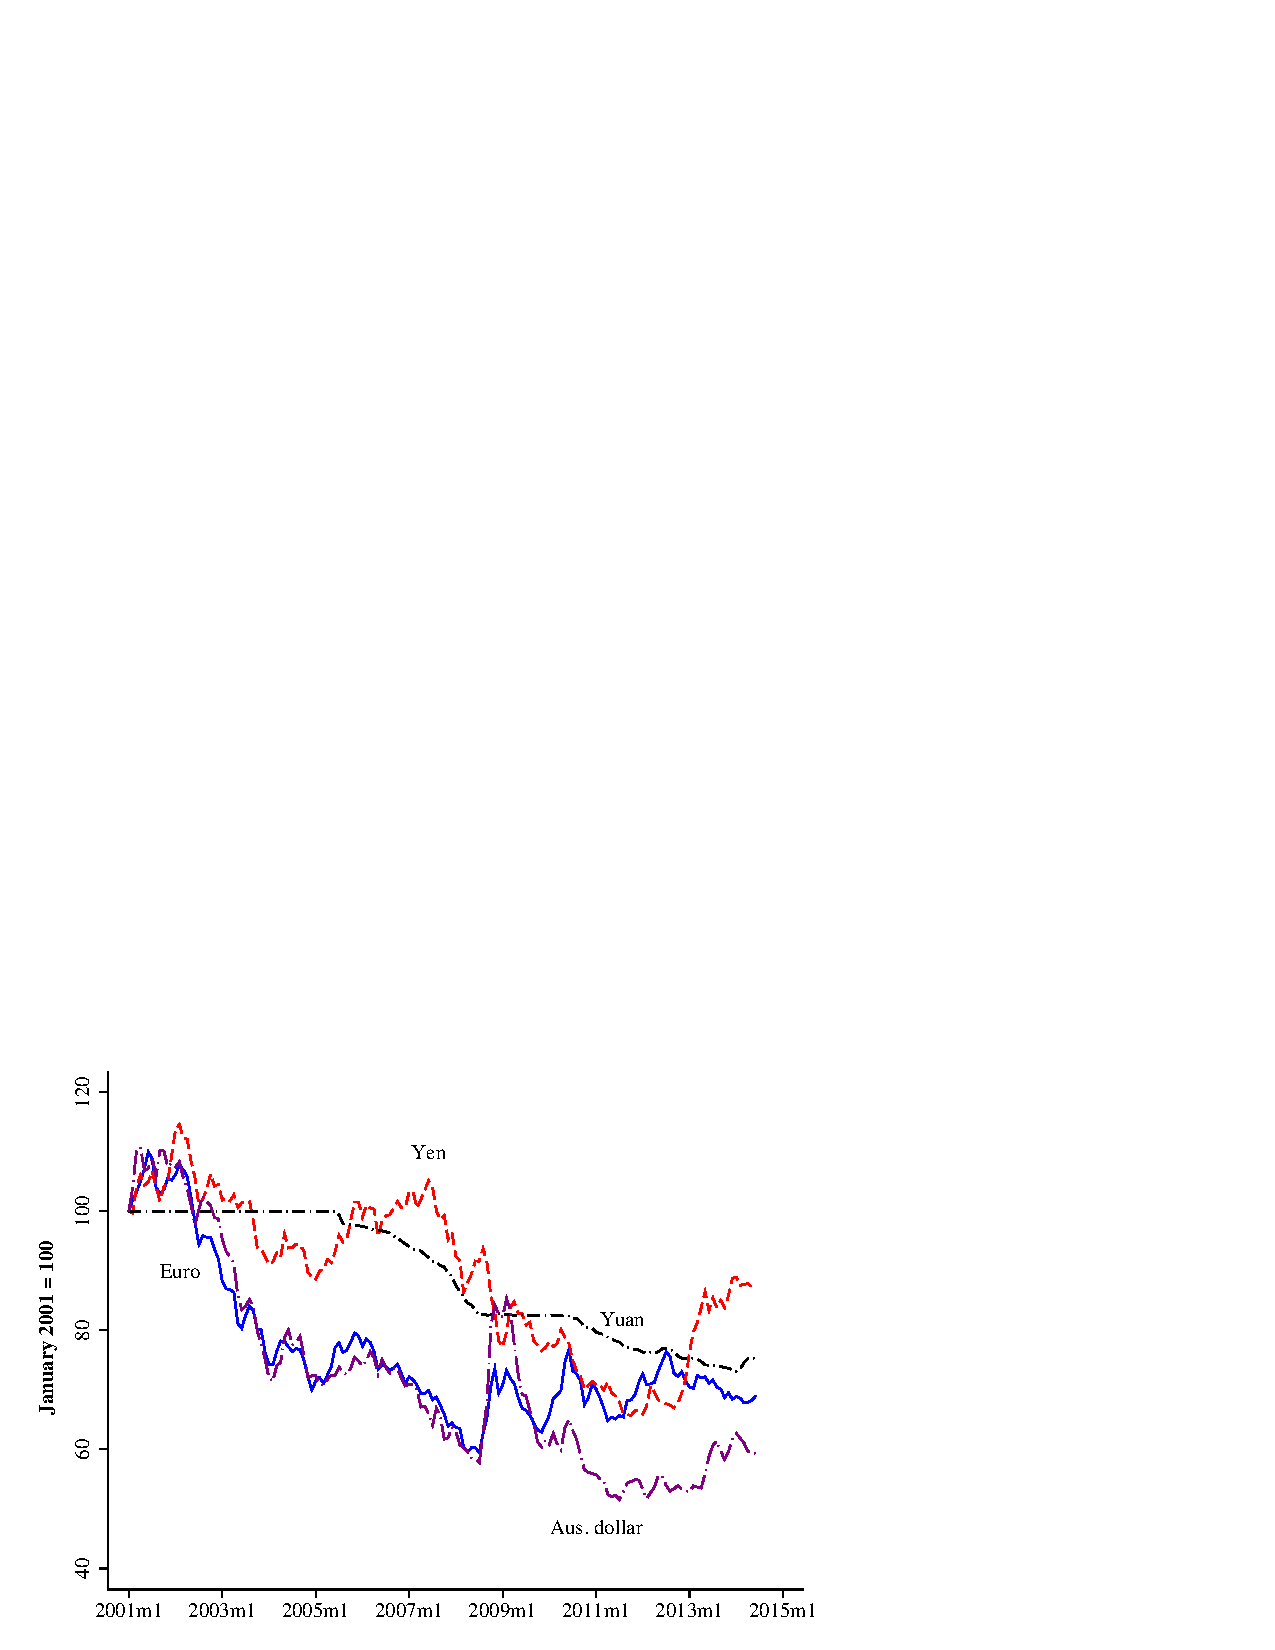
\includegraphics[width=0.8\textwidth]{\figpath Figures/exchange.pdf}
\end{figure}
%


\section{Purchasing-power parity \index{purchasing power parity (PPP)}
}

So we've seen that exchange rates move around.
But can we say anything about why?
We can't say much about short-term movements,
but here's a theory that gives us a long-term anchor
for the real exchange rate.
It's a helpful benchmark.

The idea is to compare prices of goods.
Suppose that exchange rates adjusted to equate prices across countries.
The logic is arbitrage:  If a good is cheaper in one
country than in another, then people would buy in the cheap country
and sell in the other, taking a profit along the way.
This process will tend to eliminate the difference in prices,
either through changes in the exchange rate or in the prices themselves.

Consider wine.
Suppose that a bottle of (some specific) wine costs $p=26$ dollars in New York,
and $p^*=20$ euros in Paris.
Are the prices the same?
If the exchange rate is $e=1.3$ dollars per euro,
then the New York and Paris prices are the same once we express them
in the same units.
More generally, we might say that
\begin{eqnarray*}
    p &=& e p^* .
\end{eqnarray*}
We refer to this relation as the {\it law of one price \index{law of one price} \/}:
that a product should sell for the same price in two locations.
An even better example might be gold,
which sells for pretty much the same price in
New York, London, and Tokyo.

If the law of one price works for some products,
there are many more for which restrictions on
trade (tariffs or quotas), transportation costs,
or other ``frictions'' prevent arbitrage.
Agricultural products, for example, are protected in many countries,
leading to substantial differences across countries
in the prices of such basic commodities as rice, wheat, and sugar.
Cement faces substantial shipping costs, even within countries.
Many services (haircuts, dry cleaning, medical and legal services)
are inherently difficult to trade,
and often protected by regulation, as well.

{\it The Economist\/}, with its usual flair for combining insight
with entertainment, computes dollar prices of the Big Mac around the
world.
The idea is that it's the same product everywhere, so differences
in prices reflect deviations from the law of one price.
In July 2014, Big Mac prices were \$4.80 in the US,
\$4.95 in the Euro Zone, \$3.64 in Japan, \$2.57 in Argentina,
and \$2.73 in China. These price differences vary
widely over time. For example, In January 2006, Big Mac prices  were \$3.15 in the US,
\$3.55 in the Euro Zone, \$2.19 in Japan, \$2.50 in Argentina,
and \$2.45 in China. Perhaps it's no surprise that the law of one price doesn't hold --- you can imagine the mess involved in trying to arbitrage price
differences.
But it's a good illustration of international price differences
more generally.


Despite such modest encouragement,
the first-cut theory of exchange rates is based on an application of
law-of-one-price logic to broad baskets of goods.
The so-called theory of purchasing power parity (PPP)
is that local and foreign price indexes ($P$ and $P^*$, say)
are linked through the exchange rate:  $ P \approx e P^* $ or
\begin{eqnarray}
    \mbox{\it RER\/} &=& eP^* /P \;\;\approx\;\; 1.
    \label{eq:ppp}
\end{eqnarray}
The approximation symbol suggests that we don't expect this to be perfect.
In the most common applications, the price indexes are CPIs
(consumer price indexes\index{price index!consumer price index (CPI)}),
and we refer to the measure of the real exchange rate as CPI-based.
If this doesn't work for specific goods, why might we expect it to hold
for average prices of goods?
One reason is that, for any pair of countries,
we might see as many products that are ``overpriced"
as there are products that are ``underpriced."
When we average, these deviations could offset each other, but,
in fact, they don't. If prices of some goods are cheaper abroad, then prices
of other goods tend to be, too.

What limited success we have comes in the long run.
As an empirical matter,
deviations from PPP tend to average out over time.
Sometimes prices are higher in Paris, sometimes higher in New York,
but, on average, prices are roughly comparable.
Prices are lower, on average, in countries with lower GDP per capita, but here, too, large fluctuations in the real exchange rate tend to disappear
with time.
How much time do we need for this to work?
At least several years.
If you're thinking of going to Paris next month,
there's little reason to expect that we'll be closer to PPP by then.
Maybe we will, maybe we won't; it's a tossup.


Real exchange rates computed this way are often used to judge whether
a currency's price is reasonable.
If the prices are lower at home than abroad ($\mbox{\it RER\/} > 1$),
we say the (home) currency is {\it undervalued\/}.
If prices are higher at home ($\mbox{\it RER\/} < 1$),
we say the currency is {\it overvalued\/}.
Over- and under-valued here means relative to our theory of PPP.
We can do the same thing with the Big Mac index.
We saw earlier that Big Macs were cheaper in China than in the US, so we might say that the dollar is overvalued relative to the yuan. Over time, we might expect most of these ``misvaluations'' to decline.
Experience suggests, however, that any such adjustment will take many years.
Our best estimates are that about half the difference from PPP will disappear
in five years. We can do the same thing with CPIs, with one difference: Since CPI are indexes, we don't know the absolute prices. The standard approach is to find the mean value of the real exchange rate
(or its logarithm) and judge under- or overvaluation by comparing the
real exchange rate to its mean, rather than one.


\section{Depreciation and inflation}

We can express the same theory in growth rates,
with the result that the change in the exchange rate
(the depreciation \index{exchange rate!depreciation} of the currency)
should equal the difference in the two inflation rates.
Simply put, if one country has a higher inflation rate than another,
then we would expect its currency to fall in value
by the difference.
That's not true over short periods of time,
but it's reasonable guide over longer periods of time.
Countries with high inflation rates find
that their currencies fall in value as a result.

Here's how that works.
The PPP relation  equation (\ref{eq:ppp}), implies that
\begin{eqnarray*}
    e_t &=& P_t/P_t^* .
\end{eqnarray*}
(Feel free to put $\approx$ here if you prefer.)
If we take (natural) logs of both sides, we have
\begin{eqnarray*}
    \ln e_t &=& \ln P_t - \ln P_t^* .
\end{eqnarray*}
If we take the same equation at two different dates,
we have
\begin{eqnarray*}
    \ln e_{t+1}-\ln e_{t} &=&
        (\ln P_{t+1}-\ln P_{t}) - (\ln P^{*}_{t+1}-\ln P^{*}_{t}) \\
                &=& \pi_{t+1} - \pi^*_{t+1} .
\end{eqnarray*}
In words:  The depreciation rate equals the difference in the inflation rates.
It's simply PPP in growth rates.


Does this work?
It's pretty good for long-run averages (five to ten years or more),
but like everything we know about exchange rates,
not very useful for short-term movements outside very
very-high-inflation situations.

\begin{figure}[ht]
    \caption{Venezuelan depreciation and inflation differential.}
    \label{fig:venezuela}
    \centering
    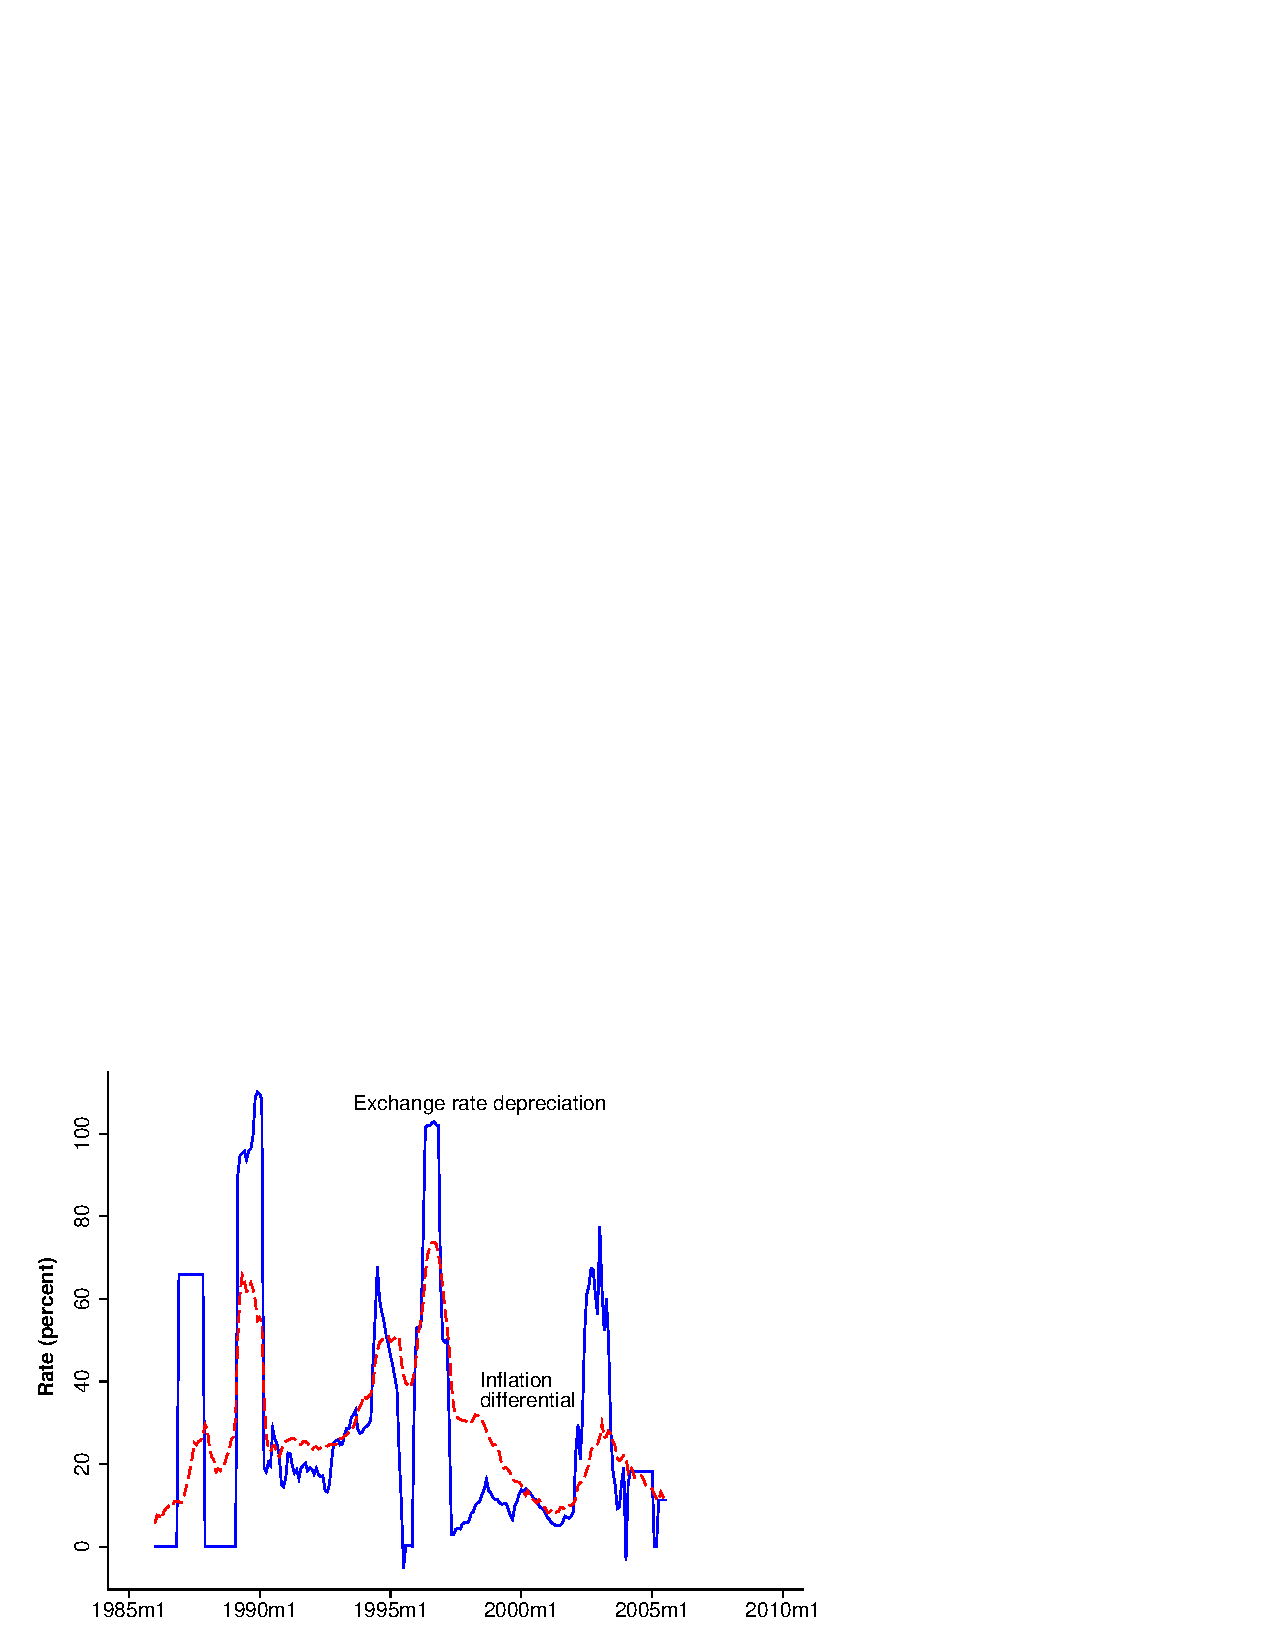
\includegraphics[width=0.8\textwidth]{\figpath Figures/venezuela.pdf}
\end{figure}

By way of example, consider the exchange rate between the Venezuelan
Bolivar and the US dollar. Between January 1985 and January 2006,
Venezuela's average annual inflation rate was 30 percent, as opposed to
the US's 2.9 percent. In the same period, the Bolivar
depreciated at the average yearly rate of 27.9 percent, i.e. only .8 percent
more than implied by the PPP condition. In the short run, however,
deviations from PPP are the norm.
Figure~\ref{fig:venezuela} shows that this has definitely been the
case for the Bolivar: There have been plenty of periods in which
exchange-rate depreciation did not closely track the inflation
differential with the United States. In some instances, in
particular in the late 1980s, the deviations were due to the central
bank's attempt to keep the exchange rate constant.
In other cases (the early 1990s, for example), the deviations
probably had nothing to do with central bank \index{central bank} interventions.

%
In developed countries, it's not unusual to see deviations of
the real exchange rate from one of 30-40 percent in either direction.
Figure~\ref{fig:us_euro} shows this for the dollar-euro.
\begin{figure}[ht]
    \caption{Dollar versus euro and inflation differential.}
    \label{fig:us_euro}
    \centering
    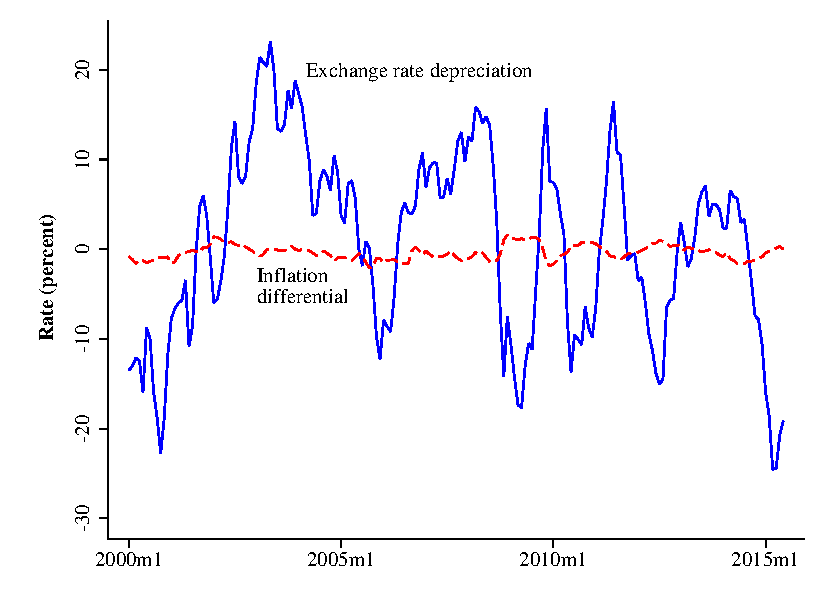
\includegraphics[width=0.8\textwidth]{\figpath Figures/us_euro.pdf}
\end{figure}
%
This picture is typical of developed countries: Inflation differentials are relatively small,
so changes in the real and nominal exchange rates are almost equal.
These deviations from PPP tend to disappear with time,
but, as we saw earlier, they go away slowly.


\section{Interest rate parity and the carry trade \index{interest rate parity}}

%  ?? change
%  interest diff and uip
%  carry trade and predictions

Exchange rates also play a role in interest rate differences across
countries. In June 2004, for example, three-month eurodollar deposits
paid interest rates of 1.40 percent in US dollars, 4.78 percent in British
pounds, 5.48 percent in Australian dollars, and 2.12 percent in euros. If
international capital markets are so closely connected, why do we see
such differences?  The answer is that these returns are
expressed in different currencies, so they're not directly comparable.\index{interest rate|(textbf}

Let's think about how prices of currencies show up in interest rate
differentials. We'll start with a relation called {\em covered
interest parity},  \index{interest rate parity!covered interest parity}
which says that interest rates denominated in
different currencies are the same once you ``cover'' yourself
against possible currency changes.  The argument follows the
standard logic of arbitrage used endlessly in finance.  Let's
compare two equivalent strategies for investing one US dollar for three
months. The first strategy is to invest one dollar in a three-month
eurodollar deposit (with the stress on ``dollar''). After three
months, that leaves us with $(1+i/4)$  dollars, where $i$ is the
dollar rate of interest expressed as an annual rate.

What if we invested one dollar in euro-denominated instruments? Here
we need several steps to express the return in dollars and make it
comparable to the first strategy. Step one is to convert the dollar
to euros, leaving us with $1/e$ euros
($e$ is the spot exchange rate --- the dollar price of one euro).
Step two is to invest this money
in a three-month euro deposit, earning the annualized rate of return
$i^{*}$. That leaves us with $(1+i^{*}/4)/e$ euros after three
months. We could convert it at the spot rate prevailing three months
from now, but that exposes us to the risk that the euro will fall.
An alternative is to sell euros forward at price $f$. In three
months, we will have $(1+i^{*}/4)/e$ euros that we want to convert
back to dollars. With a three-month forward contract, we arrange now
to convert them at the forward rate $f$ expressed, like $e$, as
dollars per euro. This strategy leaves us with $(1+i^{*}/4)f/e$
dollars after three months.

Thus, we have two relatively riskless  strategies, one yielding
$(1+i/4)$, the other yielding $(1+i^{*}/4)f/e$. Which is better?
Well, if either strategy had a higher payoff, you could short one
and go long on the other, earning extra interest with no risk.
Arbitrage will tend to drive the two together:
\begin{equation}
                            (1+i/4) \;\;=\;\; (1+i^{*}/4)f/e.
                            \label{eq:cip}
\end{equation}
We call (\ref{eq:cip}) {\it covered interest parity\/}.
Currency traders assure us that covered interest parity
is an extremely good approximation in the data, except in extreme periods of liquidity,
such as a financial crisis. The only difference between the left and right sides is a bid-ask spread,
which averages less than 0.05 percent for major currencies.


A related issue is whether international differences
in interest rates reflect differences in expected depreciation rates.
Does the high rate on Aussie dollars (AUD)
reflect the market's assessment that
the AUD will fall in value relative to (say) the euro?
To see how this works, suppose
that we converted the proceeds of our foreign investment
back to local currency at the exchange rate prevailing
in three months.  Our return would then be
\[
                            (1+i^{*}/4) e_{3}/e ,
\]
where $e_3$ is the spot exchange rate three months in the future.
This investment is risky, since we don't know what the
future exchange rate will be, but we might expect
it to have a similar expected return to a local investment.
That is,
\begin{equation}
          (1+i/4) \;\;=\;\; (1+i^{*}/4) E (e_{3})/e ,
          \label{eq:uip}
\end{equation}
where $E(e_3)$ is our current expectation
of the exchange rate in three months.
This relation is an application of the expectations hypothesis to
currency prices (the forward rate equals the expected future spot rate)
that is commonly referred to as {\it uncovered interest parity\/}. \index{interest rate parity!uncovered interest parity}


In fact, uncovered interest rate parity doesn't work.
It implies that high-interest-rate currencies depreciate,
when, in fact, they appreciate (increase in value) on average,
making them potentially good (if risky) investments.
If $i>i^*$, we invest at home.  If $i<i^*$, we invest abroad,
expecting to pocket not only the higher interest rate but
an appreciation of the currency ($e_3>e$).
That's the essence of what is called the ``carry trade.''
Why this investment opportunity persists remains something of a mystery to
academics and investors alike.

Two fine points:  (i)~This feature of the data does not apply to
the currencies of developing countries, where higher interest rates
typically do imply future depreciation.
That is, uncovered interest parity   works better here.
(ii) In developed countries, forecasts of exchange-rate changes based on interest differentials have an $R^2$ of 0.05 or less.
That's still useful for investment purposes,
but leaves most of the variance of exchange-rate changes unexplained.


\section{Predicting exchange rates}

Let's summarize what we've learned about movements in exchange rates:
%
\begin{itemize}
\item PPP works reasonably well over long periods of time,
but has little empirical content over periods of less than a few years,
and virtually none over periods under a year.

\item Interest rate differentials have some forecasting power,
with high-interest-rate currency increasing in value, on average,
but they leave most of the variance of exchange-rate movements
 unexplained.
\end{itemize}
%
Can we do better than this?
A little, but probably no more than that.
It's extremely hard to forecast exchange rates better than
a 50-50 bet on up or down.
Interest differentials do a little better, but only a little. We may be able to do better still
using more complex theory or personal judgment about policy,
but years of failure suggest that
it's very hard to beat a random walk consistently.



\section*{Executive summary}

%\setlength{\leftmargini}{.5\oldleftmargini}
\begin{enumerate}
\item In the long run, exchange rates tend to
equalize prices of products across countries (PPP).

\item In the short run, exchange-rate movements are large
and unpredictable.
\end{enumerate}
%\setlength{\leftmargini}{\oldleftmargini}


\section*{Review questions}

%\setlength{\leftmargini}{.5\oldleftmargini}
\begin{enumerate}
\item Purchasing power parity for Big Macs.
The Economist reports the following data for
local prices of Big Macs and US dollars in July 2011:
%
\begin{center}
\begin{tabular}{lccc}
\toprule
        & Big Mac Price  &  Exchange Rate    \\
        &(Local Currency)&(LCUs per Dollar)   \\
        &  (A)  &  (B) \\
\midrule
Argentina       &  20.0  &  4.13  \\
Brazil          &  9.50  &  1.54 \\
India           &  84.0  &  44.4   \\
United States   &  4.07  &  1.00   \\
\bottomrule
\end{tabular}
\end{center}
LCUs are ``local currency units.''


\begin{enumerate}
\item What is the dollar price of a Big Mac in each of these locations?
\item In what ways is the ratio of USD Big Mac prices similar to the real exchange rate?
\item What exchange rates for the first three currencies would
equate the dollar prices of Big Macs in other countries to the US price?
How is this related to PPP?
\item How much are the first three currencies over or undervalued
relative to the US dollar?
\end{enumerate}

Answer.  The calculations are summarized in
%
{\small
\begin{center}
\begin{tabular}{lccc}
\toprule
        & Big Mac   &  Big Mac  & Overvaluation\\
        &  (USD)&   (Ratio) &  (percent)\\
        & (C) & (D) & (E)  \\
\midrule
Argentina       &  4.84 &  4.91  &  19\\
Brazil          &  6.17 &  2.33  & 51\\
India           &  1.89 &  20.64 & $-53$\\
United States   &  4.07 &  1.00  & 0.0\\
\bottomrule
\end{tabular}
\end{center}
}

\begin{enumerate}
\item Dollar prices of Big Macs are reported above as column (C),
computed as (A)/(B).

\item The relative price of Big Macs is like a real exchange rate.
The real exchange rate is the ratio of prices converted to a common currency:
\begin{eqnarray*}
    \mbox{\it RER\/}  &=&  eP^*/P .
\end{eqnarray*}
Usually we use prices indexes for $P$ and $P^*$, here we use prices of Big Macs.

\item Mathematically, we set $\RER$ equal to one (the PPP condition)
and solve for $e = P/P^*$.
In the table, we computed this as the ratio of entries on column (A) to the US
entry in the same column.
That gives us a PPP benchmark for what the exchange rate should be.

\item If we compare our calculation of the PPP exchange rate in (c) to the actual,
we can see how far off we are.
In the table, we compute ``overvaluation'' as the percentage difference between
true exchange rates and our PPP calculation:  {\tt 100*[(D)/(B)-1]}.
We see that the Brazilian real is overvalued (Big Macs are expensive there)
and the Indian rupee is undervalued (Big Macs are cheap there).
\end{enumerate}

\item Forecasting the euro.
Suppose the euro is ``overvalued'' in PPP terms relative to the
dollar (goods are more expensive in Europe) and Euro Zone short-term interest rates
are slightly above US interest rates.
Given these facts, how would you expect the euro/dollar exchange rate to change over the next 6 months?  6 years?
How good is each of these informed guesses?

Answer.  Purchasing power parity is a long-run ``anchor'' for the
exchange rate:  if prices of goods and services in the Euro Zone
are higher than those in the US, when expressed in a common currency,
we'd expect the euro to fall in value relative to the dollar
--- eventually.
This is pretty much useless over a period as short as 6 months,
but has some content over 6 years.
More useful in the short-run is the interest differential.
Since the Euro interest rate is higher, we'd expect the euro to increase in value.
Neither works well:  an $R^2$ of 0.05 would be good over
periods of a few months.\index{interest rate|)}
\end{enumerate}
%\setlength{\leftmargini}{\oldleftmargini}


\section*{If you're looking for more}

\href{http://research.stlouisfed.org/fred2/}{FRED}
has exchange rates for many countries.
So does the
\href{http://www.federalreserve.gov/releases/h10/hist/}{Fed};
search:  ``fed exchange rates.''

The Economist's
\href{http://www.economist.com/content/big-mac-index}{Big Mac index}
(search: ``big mac index'')
is the center of a nice web site on exchange-rate data and issues.

Deutsche Bank's
%\href
%{http://www.deutsche-bank.de/presse/en/releases_761.shtml}
{\it Guide to Exchange-Rate Determination\/} is a terrific
summary of what we know about exchange rates from a
bond \index{bond} and currency trader's perspective.




\section*{Symbols and data used in this chapter}

\begin{table}[H]
\centering
\caption{Symbol table.}
\begin{tabular*}{0.98\textwidth}{l@{\extracolsep{\fill}}l}
\toprule
Symbol & Definition \\
\midrule
$e$      &Spot exchange rate = home currency price of foreign currency\\
$f$      &Forward exchange rate \\
$P$     &Domestic price level\\
$P^*$    &Foreign  price level\\
$\mbox{\it RER\/}$  & Real exchange rate $= eP^*/P$  \\
$\pi$     &Domestic inflation\\
$\pi^*$     &Foreign inflation\\
$i$     &Domestic nominal interest rate \\
$i^*$    &Foreign nominal interest rate \\
${E}(x)$    &Expected value of a variable $x$\\
\bottomrule
\end{tabular*}
\end{table}

\begin{table}[htb]
\centering
\caption{Data table.}
\begin{tabular*}{0.98\textwidth}{l@{\extracolsep{\fill}}l}
\toprule
Variable & Source\\
\midrule
USD/euro exchange rate    &EXUSEU\\
Yuan/USD exchange rate    &EXCHUS\\
Yen/USD exchange rate    &EXJPUS\\
USD/UK pound exchange rate    &EXUSUK\\
USD/AUD exchange rate    &EXUSAL\\
Venezuela/USD exchange rate    &EXVZUS\\
Real trade-weighted USD index (broad)    &TWEXBPA\\
US consumer price index
    &CPIAUCSL\\
Euro area harmonized consumer price index
     &CP0000EZCCM086NEST\\
\bottomrule
\addlinespace
\end{tabular*}
\begin{minipage}{0.98\textwidth}
\footnotesize{To retrieve the data online, add the identifier from the source column to \url{http://research.stlouisfed.org/fred2/series/}.  For example, to retrieve the dollar-euro exchange rate, point your browser to \url{http://research.stlouisfed.org/fred2/series/EXUSEU}}
\end{minipage}
\end{table}

\chapter{Exchange-Rate Regimes}\label{chp:fxr}
\hypertarget{fxregimes}{}

%No extra lines here.
\textbf{Tools:} Central bank balance sheet.

\textbf{Key Words:} convertibility; capital mobility; capital controls; fixed and flexible exchange rates;
foreign exchange reserves; sterilization.

\textbf{Big Ideas:}
%\vspace{-0.1in}
\begin{itemize}
\item Countries adopt different exchange rate regimes: fixed, floating, and in between.
\item The trilemma limits our policy options:  we can choose only two of
(i)~fixed exchange rate, (ii)~free flow of capital,
and (iii)~discretionary monetary policy.
\item Fixed exchange-rate regimes must be defended through open market operations
and are vulnerable to speculative attack.
\end{itemize}

\rule{\textwidth}{1pt}

The term ``exchange-rate regimes'' refers to the various
arrangements that governments around the world make about
international transactions.
We'll see (i)~how central banks intervene
in currency markets to fix the price
and (ii)~how such fixed exchange-rate systems sometimes blow up.


\section{A catalog of foreign-exchange arrangements \index{exchange rate regime}}

Governments follow a wide range of policies toward their currencies.
One aspect of policy is whether people and businesses can freely
exchange their local currency for another:
whether the currency is {\it convertible\index{exchange rate regime!convertibility}\/}.
The US dollar, for example, is convertible.
You can walk into most banks in New York and use dollars to buy dozens of foreign currencies.
Or you can use your credit card abroad and have the currency transaction
done for you.
The renminbi, however, has limited convertibility.
You need approval from the Chinese central bank \index{central bank} to buy or sell Chinese currency.

A related issue is {\it capital controls\/}: \index{exchange rate regime!capital controls}
whether the government restricts movements of capital (funds)
in and out of the country.
In the US, capital is generally free to move in and out of the country,
although there are restrictions on foreign ownership of companies
in some industries (banks, media, airlines).
In China, there are limits on foreign investments that vary (as in the US)
by industry and type (direct investment is easier than buying securities).
And there are restrictions that limit the amount of money that Chinese citizens can take out of the country.
These controls are typically enforced through convertibility:
since you can't convert renminbi to (say) dollars, you can't
take it out of the country.


There's nothing unusual about this.
Many countries limit convertibility and capital flows,
particularly during times of stress.
Malaysia imposed capital controls during the Asian crisis of 1997,
and Argentina did the same in 2002.

Another aspect of foreign-exchange policy
is whether the price of the currency is set by the government,
allowed to float freely, or something in between.
If the price is determined in a free market, we say that we have a
{\it flexible\/} or {\it floating\/} exchange-rate regime. \index{exchange rate regime!flexible exchange rate}
\index{exchange rate regime!floating exchange rate}
If the government sets the price, we say it has a
{\it fixed\/} or {\it pegged\/} exchange-rate regime. \index{exchange rate regime!fixed exchange rate}
\index{exchange rate regime!pegged exchange rate}
A {\it managed float\/} is somewhere in between. \index{exchange rate regime!managed float}


\section{Fixed exchange rates\index{exchange rate regime!fixed exchange rate}}

Many countries have fixed exchange-rate regimes of one sort or other.
Colombia uses US dollars, so its currency is fixed by design. %We say that Colombia has ``dollarized.''
The countries of the European Monetary Union use a common currency, the euro.
Other countries have their own currencies, but intervene to
fix the price.
Probably the most prominent current example is the Chinese renminbi,
which has been quasi-fixed for more than a decade.


How does a central bank \index{central bank} set the exchange rate if the currency
 is convertible?
Can it simply announce a rate?
Probably not.
You can state a price, but you can't make people trade at it.
You could claim, for example, that your apartment is worth
\$10m, but if no one is willing to buy it for that price,
the statement is meaningless.
For the same reason, a central bank \index{central bank} must back up its
claim to fix the exchange rate by buying and selling as much
foreign currency as people want at the stated price.


Let's think through how this might work.
Suppose the New York City government decided to fix the price of beer at \$2 a six pack (cheap even if you live outside NYC).
It supports this price by buying or selling
any amount at the quoted price.  Can they keep the price this low?
Our guess is that at this price,
beer makers would not find it profitable to make any
(at least not any that we'd be willing to call beer).  People would then flood the government with requests for beer, which the government would
not be able to meet.  When the government reneged on its promise to buy or sell at \$2, the price
would rise above \$2 to its market level, either officially or on the black market.
Unless the government has enough beer to back up the price,
the system will collapse.
Alternatively, suppose that the government set the price at \$20.
Beer makers would flood the government with beer at this price, leaving the
government with a huge surplus.  This is roughly what Europeans do with agriculture, where artificially high prices have left the EU with
``mountains of butter," ``lakes of wine," and so on.
The point is that the government can fix a price
only if it is willing and able to buy and sell at that price --- or outlaws market transactions altogether.

The same logic applies to currencies.
If the People's Bank of China were to support an excessively high price for
the renminbi, then it would be flooded with offers from traders
selling renminbi for (say) dollars.
Its balance sheet would look something like this:
%
\begin{center}
\begin{tabular}{lr|lr}
               Assets  &     &     Liabilities                     \\
               \hline
               FX Reserves &  20 &     Money &  200   \\
               bonds   & 180 & \\
\end{tabular}
\end{center}
%
We made these numbers up, but they give us the right idea.
The central bank \index{central bank} has the usual liabilities,
``money" and government bonds \index{bond},
and also holds some foreign currency reserves,
which you might think of as dollars.
The PBOC intervenes in the currency market by trading renminbi for dollars,
and vice versa, depending on market conditions.


Suppose, for example, that Nike wanted to convert
\$2m to renminbi to build a new plant in China.
It would do this through a Chinese bank.
If the bank had no countervailing trades, it would
go to the PBOC and exchange the \$2m for renminbi at the going rate --- say ten yuan per dollar, to make the arithmetic simple.
The PBOC's balance sheet would then show an increase of
20m yuan worth of foreign currency
and a comparable increase in its monetary base:
%
\begin{center}
\begin{tabular}{lr|lr}
               Assets  &     &     Liabilities                     \\
               \hline
               FX Reserves &  40 &     Money &  220   \\
               bonds \index{bond}  & 180 &
\end{tabular}
\end{center}
%
Note that the transaction doesn't make the PBOC any richer.
%It's simply a portfolio shift.
Its net worth is unchanged,
since it has exchanged assets with equal value.

The difference, then, between fixed and flexible exchange-rate regimes
is that the former obligates the central bank \index{central bank} to buy and sell
currencies at the stated price.

\section{Sterilization \index{exchange rate!sterilized intervention} \index{intervention} \index{monetary policy!sterilization}}

You might have noticed that when a central bank \index{central bank} buys and sells foreign currency,
its money supply changes.
In the example above, the purchase of 20 worth of foreign currency increased the money supply by the same amount.
It's automatic:  when the central bank \index{central bank} purchases foreign currency, it offers domestic
currency in return.

Central banks \index{central bank} often want to reverse this impact of foreign exchange intervention
by engaging in an offsetting open market operation.
We refer to this as {\it sterilization\/}. \index{intervention} \index{exchange rate!sterilized intervention}

In our example, the central bank \index{central bank} would like to reduce the money supply by 20,
offsetting the impact of buying foreign currency.
It does so with an open market sale of government bonds. \index{bond}
The sale of bonds \index{bond} is paid for in local currency, which is now held
by the central bank \index{central bank}.
Its balance sheet is now
%
\begin{center}
\begin{tabular}{lr|lr}
               Assets  &     &     Liabilities                     \\
               \hline
               FX Reserves &  40 &     Money &  200   \\
               bonds  & 160 &
\end{tabular}
\end{center}
%
In China's case, this has happened to such an extent that the bond \index{bond}
position is negative:  the PBOC is an issuer of bonds\index{bond}, not an investor.


\section{The trilemma \index{exchange rate regime!trilemma of open-economy monetary policy} }

Exchange-rate policy is, evidently, a dimension of monetary policy
since it involves management of the central bank's \index{central bank} balance sheet.
Is it another tool a central bank \index{central bank} can use to manage the economy?

Both logic and experience tell us that the central bank's \index{central bank} choices are limited.
The sharpest example is the {\it trilemma\/}.
You can choose, at most, two of the following:
% ?? honest, smart, get elected
\begin{itemize}
\item fixed exchange rate\index{exchange rate regime!fixed exchange rate|(textbf}
\item free international flow of capital
\item discretionary monetary policy \index{monetary policy!policy discretion}
\end{itemize}
If you try for all three, something will give, probably the exchange rate.

The US lets the exchange rate float, which allows it to have a discretionary
monetary policy and free movements of capital.
China limits the international flow of capital,
which allows it to have a fixed exchange rate and some degree of monetary policy discretion.
The UK, in 1992, tried for all three, and it blew up, driving them out
of the European Monetary System, the precursor of the European Monetary Union.
%Mexico let its real exchange rate appreciate in 1994,
%only to see it depreciate sharply at the end of the year.


\section{Exchange-rate crises}

As a matter of experience, fixed exchange-rate systems often collapse ---
sometimes spectacularly --- when the central bank \index{central bank} runs out of reserves.

We can illustrate the mechanics with the central bank's \index{central bank} balance sheet.
Suppose that it looks like the one above, with ``fx reserves'' of 40.
And suppose, further, that investors
would like to exchange 50 worth of pesos for the same value in dollars.
Once the central bank \index{central bank} runs out of dollars, it can no longer support
the exchange rate, which becomes (more or less automatically) floating.

It's the same issue we illustrated earlier with beer: If people would prefer to buy foreign currency at the official
exchange rate,
and the currency is convertible,
the central bank \index{central bank} may find that its supply of foreign reserves is not
enough to meet the market demand.
(The market for currencies is enormous, so you need a lot of reserves.)
For that reason, currency traders often look closely at the central bank's \index{central bank}
foreign currency reserves to measure its ability to maintain a fixed rate.
\index{exchange rate regime!speculative attacks}

What invites ``speculative attacks" on a currency with a fixed exchange
rate? Often, it's a problem of \hyperref[sec:time_cons]{time consistency}.\index{time consistency} A fixed exchange rate is a
policy promise to exchange one currency for another at a specified price
without limit into the future. If investors today expect that a future
policymaker will alter that price, what will stop them from selling the
``expensive" currency today? In a foreign-exchange market that transacts
about four trillion dollars daily, few governments have adequate foreign
reserves to fend off a run on a fixed exchange rate.

One classic currency run occurred in 1992 in the United Kingdom.
As part of the European Exchange Rate Mechanism (ERM), the UK had effectively
fixed its currency, sterling, to Germany's Deutsche Mark (DM).
But Germany was in its post-unification economic boom and needed
high interest rates to limit inflation, while the UK was in a deep recession
and needed low interest rates. Doubting that UK policymakers
would keep interest rates high just to maintain the fixed exchange rate,
speculators sold sterling. They made a fortune when the UK exited
the ERM in September 1992 and sterling plunged versus the DM.\index{interest rate}

You might ask: Should the UK have considered capital controls   instead of
devaluing sterling? One practical obstacle was that any hint of controls
would have further encouraged investors to flee sterling
before they could no longer do so. Where time consistency is lacking --- in this case, in currency policy --- instability often follows.\index{time consistency}

There's a big-picture question lurking behind the scenes here:
whether fixed exchange rate regimes reduce volatility.
With flexible rates, we tend to see a lot of short-run volatility.
With fixed exchange rates, short-run volatility is low most of the time,
but we occasionally have spikes in volatility when the system collapses.
Neither seems completely appealing, but that's the choice we're given.


\section{Strong fixes}

The tendency for fixed exchange rates to blow up has led to two
competing lines of thought.
One is to let them float --- let the pressure off, so to speak.
The other is to reinforce the fixed-exchange-rate system and nail the lid down tighter.
Nothing has proved foolproof to date, but you never know.

One way to reinforce a fixed exchange rate is with a currency board.
The idea is to start off with a large reserve of foreign currency
and limit issues of domestic currency to this amount.
That way, you should not run out of foreign currency when people trade
in their local currency.
Argentina set up a system like this in the 1990s, and established
an exchange rate of one dollar per peso.
But it was dissolved in a currency crisis ten years later.
Hong Kong has had such a system since 1983, with the Hong Kong dollar
pegged to the US dollar.
As a result, interest rates in Hong Kong mirror those in the US:
it has, in a sense, inherited US monetary policy.\index{interest rate}


A more extreme arrangement is a common currency.
EMU (the euro area) is the most ambitious effort along these lines to date.
But it has been under stress for years, and it remains unclear whether
it will survive in its current form.


\section*{Executive summary}

%\setlength{\leftmargini}{.5\oldleftmargini}
\begin{enumerate}
\item ``Convertibility'' and ``capital mobility'' refer to
policies limiting currency transactions and international capital flows.

\item Foreign currency reserves are an indicator of the
government's ability to maintain a fixed exchange rate.

\item The trilemma says you can have, at most, two of the following three
things:
(i)~fixed exchange rates;\index{exchange rate regime!fixed exchange rate|)}
(ii)~international capital mobility; and
(iii)~discretionary monetary policy.
\end{enumerate}
%\setlength{\leftmargini}{\oldleftmargini}

%\begin{comment}
\section*{Review questions}

%\setlength{\leftmargini}{.5\oldleftmargini}
\begin{enumerate}
\item Foreign exchange market intervention.
Use a hypothetical central bank \index{central bank} balance sheet to show how
purchases of foreign currency affect the bank's assets and liabilities. What does this purchase do to the supply of money (currency)?

Answer.  When a central bank \index{central bank} buys foreign currency,
it receives it from private owners and gives them
    domestic currency in return.
    The latter is an increase in the domestic money supply.
    Suppose, for example, that the central bank \index{central bank}
    starts with the balance sheet
    %
\begin{center}
\begin{tabular}{lr|lr}
               Assets  &     &     Liabilities                     \\
               \hline
               FX Reserves &  100 &     Money  &  200   \\
               bonds   & 100 & \\
\end{tabular}
\end{center}
%
The purchase of 25 worth of foreign currency
changes the balance sheet to
%
\begin{center}
\begin{tabular}{lr|lr}
               Assets  &     &     Liabilities                     \\
               \hline
               FX Reserves &  125 &     Money  &  225   \\
               bonds   & 100 & \\
\end{tabular}
\end{center}
%

\item Sterilization.  Suppose that the central bank has increased the money supply by purchasing foreign currency, as described above.
    How might it offset this impact on the money supply (sterilize it, so to speak)?

Answer.  It does an equal sale of bonds, accepting money in return.
If it sells 25 worth of bonds, the balance sheet changes to
\begin{center}
\begin{tabular}{lr|lr}
               Assets  &     &     Liabilities                     \\
               \hline
               FX Reserves &  125 &     Money  &  200   \\
               bonds   & 75 & \\
\end{tabular}
\end{center}
%
The net result of the two trades is that its liabilities are now more heavily weighted in foreign currency.
If the foreign currency rises, it makes money; if it falls, it loses money.
This posture is designed as protection against a sharp fall in local currency (or rise in foreign currency), and it does that.

\item Hong Kong's trilemma.
Use the trilemma to explain why Hong Kong has inherited US monetary policy.

Answer.  Hong Kong has (i) a fixed exchange rate against the US dollar and
(ii)~international capital mobility.
The trilemma then tells us that it can't have its own monetary policy.
Should they want their own monetary policy, either (i) or (ii) has to go.
\end{enumerate}
%\setlength{\leftmargini}{\oldleftmargini}


\section*{If you're looking for more}

The International Monetary Fund's
{\it Annual Report on Exchange Arrangements\/}
is the definitive guide to exchange-rate arrangements:  fixed,
flexible, capital controls, and so on.

\chapter{Macroeconomic Crises}\label{chp:cris}
\hypertarget{crises}{}

%No extra lines here.
\textbf{Tools:} Crisis triggers and indicators.

\textbf{Key Words:} Sovereign default; bank runs and panics; refinancing (rollover) risk; leverage; conditionality;
solvency and liquidity.

\textbf{Big Ideas:}
%\vspace{-0.1in}
\begin{itemize}
\item Common triggers of macroeconomic crises are sovereign debt problems, financial fragility,
and fixed exchange rates.

\item Measures related to these triggers can help identify countries in trouble:
debt and deficits, financial weakness, exchange rate regime, and so on.

\item The goals of crisis prevention and crisis management are often at odds.
\end{itemize}

\rule{\textwidth}{1pt}

Economies periodically experience {\it crises\/}:
economic downturns that are not only larger than typical recessions
but qualitatively different.
The idea is now fresh in our minds,
but similar episodes have occurred throughout recorded history.
They're less common in modern, developed countries,
but they can happen anywhere.
Like snowflakes and business cycles, no two are exactly the same,
but they share some common features.


\section{Classic crisis triggers }

There are three classic triggers of macroeconomic crises:
sovereign debt, financial fragility, and a fixed exchange rate.\index{exchange rate regime!fixed exchange rate}

\textbf{Sovereign debt problems.\index{government debt!sovereign debt}}
If investors fear that a government may not repay its debt,
the market for debt collapses, often taking the economy with it.
In the old days, wars were the standard problem.
Wars are expensive, and if investors thought the expense was more
than the government was willing or able to bear,
they would stop buying the debt.
In modern times, governments spend money on many things besides wars,
but the possibility of default remains.
Argentina in 2002 and Greece today are recent examples.
These experiences remind us that sovereign debt need not be risk-free.

The central issue with government debts is sovereignty.
If a corporation defaults, the creditors take it to court
and claim the assets.
With governments, there's no such mechanism, and the process
is sloppier as a result.

\textbf{Financial fragility.}
We know from centuries of experience that when the
financial system freezes up,
economic activity slows down sharply.
We saw that in 2008,
but the same thing happened during the Bank of England Panic of 1825,
the Baring Crisis of 1890,
the US Panic of 1907,
Japan and Scandinavia in the 1990s,
and many other occasions.
It's a feature of even advanced financial systems that they
sometimes break.

In most cases, these financial problems follow from
poor investments (real estate is a common example),
which put the solvency of financial institutions in question.
The problems tend to snowball: Worries about the viability of one firm may lead others to
reduce their lending, leading to a cycle of retrenchment
that puts even sound firms in trouble.
The word ``panic'' is apt here and stems
from the imperfect information that investors have
when deciding where to put their money.


\textbf{Fixed exchange rates.} For whatever reason, fixed exchange rates periodically
must be defended in ways that undermine the economy.
Recent examples include the UK in 1992,
Mexico in 1994,
Korea in 1997,
and Argentina in 2000.

Many crises combine several of these elements.
The countries of the euro area face all three.
In Ireland and Spain, bailing out their banks
landed the governments in financial peril.
In other countries, bank positions in government debt
or in overpriced real estate put the banking systems in peril.
Finally, the common currency eliminates exchange rate changes
as a possible correction mechanism.


\section{Crisis indicators: the checklist\index{crisis!crisis indicators} }

Crises are inherently hard to predict.
Why?
Think about cardiologists.
We understand that they can identify risk factors
(weight, high blood pressure) but cannot predict
the date of a heart attack with any precision.
Crises are worse.
Once people see a crisis on the way,
their actions tend to reinforce it:
they sell government debt,
withdraw funds from banks,
or shift their money to foreign currency.
But like a cardiologist, we can use what we know
to identify signs of trouble.


Analysts differ in the details, but most would include
the following in their ``checklist'' of crisis indicators:

%\begin{itemize}
\textbf{Government debt and deficits.}
The primary issue here is the quality of governance.
That aside, common rules of thumb include:
Worry if government
deficit is more than 5 percent of GDP or debt is more than 50 percent of GDP.
Adjust upward for developed countries, downward for developing countries
and for regional governments.
And watch out for hidden liabilities:  pensions, health care, bailouts, etc.
These are often much larger than official liabilities.

Fine points:  Worry further if debt is short-term and/or denominated in foreign currency.
Short-term debt subjects the government to refinancing (``rollover'') risk;
markets may demand better terms or refuse to refinance.
Foreign-denominated debt subjects government to risk
if currency falls in value, making the debt larger in local terms.

\textbf{Banking/financial system.}
This isn't something we've discussed,
but  analysts track leverage, duration mismatch, exposure concentration,
risk-management processes,
and nonperforming loans.
The challenge is measuring them accurately from reported information.
Some of the most troubling situations come with low-quality data.


\textbf{Exchange rate and reserves.}
Rule of thumb:  Worry if the exchange rate is fixed, or close to it,
and the currency is significantly overvalued in PPP terms
(Big Macs cost 30 percent more than in other currencies;
the real exchange rate has risen more than 30 percent in the past 2-5 years).
Worry more if foreign-exchange reserves
are low or have fallen significantly.

\textbf{Political situation.}
%Rule of thumb:  Worry if the political system seems unable or unwilling
%to deal with problems that could lead to crises.
Crises are often more political than economic.
Countries with effective governments suffer fewer crises and
deal with those that occur more effectively.
Analysts therefore look for signs that the political
system is unable or unwilling to deal with problems that might turn into crises.
Zimbabwe's hyperinflation and Argentina's debt crisis are good examples.
Or the Weimar Republic in 1920s Germany.
%\end{itemize}

All of these things generate more concern
in countries with weak institutions.
It's not an accident that Greece is in worse trouble
than France or Germany.
%Analysts often find that local politics are more important
%than the numbers to the outcome.


\section{Crisis responses\index{crisis!crisis responses}}

What should a government do when faced with a crisis?
It depends on the trigger.
Standard advice includes:

\textbf{Sovereign debt crises.}
If the problem is that the government is borrowing too much,
the answer is to stop doing it --- run primary surpluses until the debt is manageable.
Default is also an option, and saves money in the short term,
but probably raises borrowing costs in the future.
And if you go through a default, it's helpful to resolve it as quickly as possible.

IMF support is often used to cushion the blow: Contingent on progress with the deficit,
the IMF lends the government money on more attractive terms
than the market would provide.
This ``conditionality,'' as it's called,
helps reduce moral hazard (you get the money only if you behave)
and provides cover for local politicians (the IMF made us do this).
Such conditional lending can be critical in a crisis,
when high borrowing rates exacerbate the government's debt problems.
(See:  debt dynamics.)


\textbf{Financial crises.}
If the financial system is fundamentally sound (solvent) but illiquid,
the longstanding advice is for the central bank \index{central bank} to lend aggressively.
The classic quote comes from Walter Bagehot,
a 19th-century businessman and journalist:
``To avert panic, central banks \index{central bank} should lend early and freely,
to solvent firms, against good collateral, and at high rates.''
%Put simply,
%the goals of crisis prevention and crisis management
%are often at odds.


If the financial system is insolvent,
it's important to get it recapitalized and operating again.
This advice comes with more than a little irony,
as governments sometimes find themselves bailing out
precisely those banks that triggered the crisis.
The trick is to do it in ways that inflict some pain
on the bank's management and creditors
(incentives for the future) and don't bankrupt the government.
These things happen fast, so it's hard to get everything right.


\textbf{Fixed exchange rates.} Let them float.
A more controversial approach is to impose capital controls   to inhibit the
response of capital markets to a possible drop in the exchange rate.
(See:  trilemma.)
capital controls   are a dangerous tool,\index{exchange rate regime!fixed exchange rate}
because the fear of future capital controls
can generate a crisis on its own,
as investors rush to get their money out of the country.
capital controls   on inflows may, for that reason, be more attractive
than controls on outflows.


\section*{Executive summary}

\setlength{\leftmargini}{.5\oldleftmargini}
\begin{enumerate}\itemsep=0.0in
\item The classic crisis triggers are
(i)~government debt and deficits,
(ii)~a fragile financial system,
and (iii)~a fixed exchange-rate system.

\item Crises are hard to predict,
but we nevertheless have useful indicators connected to each
of the triggers.

\item Politics and institutions are central.
\end{enumerate}
\setlength{\leftmargini}{\oldleftmargini}

%\end{document}

\section*{Review questions}

\setlength{\leftmargini}{.5\oldleftmargini}
\begin{enumerate}
\item Risk and opportunity in Ghana (May 2012).
You have been asked to prepare a risk assessment for
the West African country of Ghana.
Ghana is a former British colony that has been growing rapidly
in recent years after a period of unusually stable politics.
The Economist Intelligence Unit refers to it as a ``robust democracy.''
The World Economic Forum ranked Ghana 114th (of 133)
in their Global Competitiveness Report.
They continue:
``The country continues to display strong public institutions and
governance indicators,
particularly in regional comparison.''

The EIU's Country Risk Report adds:
\begin{itemize}
\item The December 2012 elections are expected to be close.
The president, John Atta Mills, came to power promising accountability
and transparency, but  has struggled to maintain party unity
while evidence emerges of financial impropriety of some government ministers.
\item The victor faces a challenging policy environment, particularly
the fiscal situation.
\item Expectations among the population are high as production
starts at the offshore Jubilee oil field.
\item The government's decision to allow use of 70\% of future
oil revenue as collateral for borrowing is a cause for concern
if the revenue is not managed properly.
\item The Bank of Ghana (the central bank \index{central bank}) faces the twin goals of
containing inflation\index{inflation} and fostering growth.
\item The currency  ---  the cedi --- floats with occasional heavy intervention.
\end{itemize}
%
Your mission is to assess the risks to Ghana  using
the information in the table, as well as
your own good judgement and analytical skills.

\begin{enumerate}
\item  You decide to start with a fiscal assessment.
What trend do you see in government revenues and expenses?

\item You notice that neither the primary deficit nor
interest expenses are reported separately.
How would you estimate them from the numbers in the table?
What are their values for 2011?

\item Using what you know about government debt dynamics,
compute the ratio of government debt to GDP for 2011.
What factors contribute the most to the change from 2010?

\item Overall, how would you assess the risks to Ghana's economy over
the next couple of years?
\end{enumerate}

{\small
\begin{tabular}{lrrrrr}
\toprule
        & 2008 & 2009 & 2010 & 2011 & 2012 \\
\midrule
GDP growth (\%) & 8.4 & 4.0 & 7.7 & 13.6 & 7.4 \\
Inflation (\%)  & 18.1 & 16.0 & 8.6 & 8.6 & 8.5 \\
Interest rate (\%) & 20.8 & 28.8 & 22.7 & 20.5 & 20.6  \\
Govt revenue (\% of GDP)  & 16.0 & 16.5 & 19.1 & 23.4 & 22.2 \\
Govt spending (\% of GDP) & 24.5 & 22.3 & 25.5 & 27.6 & 27.7 \\
Govt budget balance (\% of GDP) & --8.5 & --5.8 & --6.5& --4.2 & --5.5\\
Govt debt (\% of GDP) & 30.6 & 33.3 & 33.9 & {\bf } & {\bf } \\ %& 36.8 & 41.6\\
Real exchange rate (index) & 81.7 & 76.3 & 81.8 & 78.1 & 74.5\\
FX reserves (USD billions) & 1.8 & 2.9 & 4.3 & 4.4 & 4.8 \\
\bottomrule
\end{tabular}
}

\medskip
Data from EIU CountryData.
The government budget balance is a surplus if positive, deficit if negative.
The real exchange rate is the price of goods in Ghana relative to the rest
of the world;
the larger the number, the more expensive goods are in Ghana.
The numbers for 2011 and 2012 are estimates.

Answer.
\begin{enumerate}
\item Trends include:
(i)~revenues and spending both rising,
(ii)~spending still ahead of revenue (there's a deficit),
and (as a direct result)
(iii)~ratio of debt to GDP rising a little
(more on that to come).

\item This is a tricky one.
Remember that interest payments in year $t$ are $ i_t B_{t-1}/Y_t$.
We get what we want from:
\begin{eqnarray*}
    i_t B_{t-1}/ Y_{t} &=& i_t (B_{t-1}/ Y_{t-1}) (Y_{t-1}/ Y_{t}) \\
           &\approx&  i_t (B_{t-1}/Y_{t-1}) /(1+g_t + \pi_t) .
\end{eqnarray*}
That gives us interest payments in 2011 of 5.7\% of GDP and
a primary deficit of $-1.5$\% (that is, a surplus).

\item The key relation is this one:
\begin{eqnarray*}
    \Delta ({B_{t}}/{Y_{t}})
            &=&
                (i_t-\pi_t) ({B_{t-1}}/{Y_{t-1}})
                - g_t ({B_{t-1}}/{Y_{t-1}})
             +    ({D_{t}}/{Y_{t}})  .
\end{eqnarray*}
We refer to the components on the right as A, B, and C.
Doing the calculations gives us

\begin{center}
\begin{tabular}{lrr}
\toprule
        &  2010 & 2011   \\
\midrule
Interest payments  &  &  4.0  \\
Component A (interest)  &  &  4.0  \\
Component B (growth)            &   & --4.6  \\
Component C (primary deficit)   &   & --1.5  \\
Total change in $B/Y$       &       & --2.1   \\
Public debt (\% of GDP)     &  33.9 & 31.8   \\
\bottomrule
\end{tabular}
\end{center}

Over this period, the ratio of debt to GDP fell by 2.1\%.
The components contributed:
interest +4.0, growth --4.6, and the primary deficit --1.5.
Note especially the growth term, the result of unusually high GDP growth in 2011.

\item This is a call to look at the checklist of crisis indicators:
\begin{itemize}
\item Government debt and deficits.
We have deficits, but there's not
much sign yet of a growth debt to GDP ratio.
One future concern might be the possibility of borrowing now against future oil
revenue.  Will any debts incurred be spent wisely?
Will the oil revenue show up?
\item Banking system.  No information provided.
\item Exchange rate and reserves.  Reserves are modest,
but with the exchange rate floating there shouldn't be much
concern about that.
\item Politics.  Always an issue,
especially with a contentious election coming
and the promise of money from oil revenue.
It's an odd fact but a true one that revenue
from natural resources is more likely to cause problems than solve them.
\end{itemize}
\end{enumerate}
Update:  In August 2014, Ghana asked the IMF for help.
The chance of default remains low, since foreign debt is backed by  oil revenue,
but the promise of oil has turned into a curse,
as it often does.



% ==============================================================================
\item Don't Cry for Me Argentina.
(We know, it's a cliche, but so is their approach to policy.)
Argentina is a seemingly endless source of entertainment to economists,
yet its economy has done well in the recent past.
GDP growth fell to 0.9\% in 2009, during the global financial crisis,
but averaged over 9\% the next two years.
Most analysts attribute this success to
favorable commodity prices and strong global demand for Argentina's commodity exports.
Additional information is provided in Table \ref{tab:argentina}.

\begin{table}[h]
\centering
\tabcolsep=0.06in
\begin{tabular}{lrrrrr}
\toprule
                & 2010 & 2011 & 2012 & 2013 \\
\midrule
Official exchange rate (pesos per USD)  & 3.90 & 4.11 & 4.54 & 5.46  \\
Inflation (\%)              & 22.9 & 24.4 & 25.3 & 20.6 \\
Foreign currency reserves (USD billions) & 52.2 & 46.4 & 43.2 & 32.2 \\
Real GDP growth (\%)        & 9.2 & 8.9 & 1.9 & 5.2  \\
Govt revenue (\% of GDP)    & 24.3 & 23.6 & 25.4 & 27.3 \\
Govt spending (\% of GDP)   & 24.1 & 25.3 & 28.0 & 30.5  \\
Public sector surplus (\% of GDP) & 0.2 & --1.7 & --2.6 & --3.2 \\
Primary balance (\% of GDP) &  1.7 & 0.3 & --0.2 & --0.8   \\
Govt debt (yearend, \% of GDP)  & & & 44.8\\
Interest rate paid on debt (\%) & 4.0 & 5.5 & 6.7 & 6.5  \\
Money market interest rate (\%) & 9.1 & 10.0 & 9.8 & 12.7 \\
\bottomrule
\end{tabular}
\caption{Economic indicators for Argentina.  Source:  EIU.}
\label{tab:argentina}
\end{table}


At the same time, the government of President Cristina Fernandez de Kirchner
continues to adopt policies that befuddle outside observers, including:
taking over private pension funds,
restricting imports and purchases of foreign currency,
attacking the press,
nationalizing the Spanish-owned oil company YPF,
imposing price controls on electricity, natural gas, and public transportation,
and subsidizing energy consumption.

The Economist Intelligence Unit reports:
\begin{itemize}
\item A US court case may eventually leave
Argentina with the unpalatable choice of repaying the ``holdouts'' (creditors that
did not participate in the 2005 or 2010 restructurings) in full --- something that it
has sworn never to do --- or falling into default with its remaining creditors.

\item According to official data, consumer price inflation remains among the highest
in emerging markets, at 10.5\% in April 2013. However, the official data are
widely discredited and we are now using estimates produced by PriceStats,
which estimates that inflation in 2012 was 25\%.

\item Double-digit inflation has generated real peso appreciation.
Foreign-exchange controls have failed to prevent an erosion of
foreign exchange reserves,
heightening the risk of an eventual devaluation.

\item The Argentine peso floats in principle, but the central bank intervenes to limit
its rate of depreciation.
In addition, foreign currency transactions are subject to a variety of controls.
For the past couple of years, the government has
been gradually tightening the ``clamp,''
an unofficial policy of discouraging purchases of dollars.
As a result, the peso's official decline has been modest,
but the unofficial ``blue market'' price of the peso is considerably lower.

\item The poor banking sector risk rating reflects weak economic activity, expansionary
monetary policies that contribute to credit risk, high risk of exchange-rate
and interest-rate volatility, and increased currency convertibility risk.

\item The ruling party fared badly in the October midterm election,
 leaving the president without enough support in Congress
 to change the constitution and run for re-election.
 Focus will now shift rapidly to the 2015 presidential race.
 The president remains alienated from almost all of the country's most influential groups,
including the unions, the media, the Catholic Church and the traditional
leaders of the Peronist party. In this context, risks to political stability will be
high. An additional risk to stability is the president's health.
\end{itemize}
%
The question is what happens next:  Could another crisis be on the way,
or has Argentina put its problematic past to rest?
Use the information provided, 
and your own experience and good judgement,
to assess the risks to the Argentina economy over the next 2-3 years.
%
\begin{enumerate}
\item By ``real appreciation'' we mean an increase in the price
of local goods relative to foreign goods ---
what is sometimes called a decline in the real exchange rate.
Use the numbers in the table to demonstrate (or disprove) real appreciation
of the peso.

\item Why do you think the central bank's foreign exchange reserves have declined?

\item How do you see government debt evolving?
Compute, in particular, the ratio of government debt to GDP at year-end 2013.
What factors contribute the most to the change in the ratio?

\item Overall, how would you rate the risk of a macroeconomic crisis in Argentina?
What are the biggest sources of concern?
\end{enumerate}

\needspace{4\baselineskip}
Answer.
\begin{enumerate}
\item
The issue is the real exchange rate
$ \mbox{\em RER\/} = eP^*/P$, where $e$ is the exchange rate
(the peso price of one dollar),
$P$ is the price of Argentine goods,
and $P^*$ is the price of American goods.
So how is the real exchange rate changing?
In words:  the combination of high inflation and
more modest currency depreciation has made Argentine goods expensive
(equivalently, foreign goods cheap).

How would you show this?
Inflation is the rate of increase in $P$,
and we see the price of Argentine goods going up rapidly, roughly 20\% a year.
In contrast, $eP^*$ is going up less:
$P^*$ is roughly flat (1-2\% inflation in the US)
and $e$ is rising (if we compute its rate of change)
5\% in 2011 and 10\% in 2012.
Thus {\it RER\/} is rising, as Argentine goods get relatively more expensive.

\item Evidently people want dollars, not pesos, and the central bank supplies
them to maintain a relatively stable exchange rate.
One possible reason:  Argentine prices are rising,
and a substantial depreciation is one way to get that.
That makes pesos less attractive, since you'd lose (relative to dollars)
if the peso falls in value.

\item The debt dynamics equation is
\begin{eqnarray*}
   \Delta (B_t/Y_t)  &=&  (i_t - \pi_t)(B_{t-1}/Y_{t-1})
                - g_t (B_{t-1}/Y_{t-1}) + D_t/Y_t .
\end{eqnarray*}
The three terms are
\begin{eqnarray*}
    (i_t - \pi_t)(B_{t-1}/Y_{t-1}) &=&  -6.3  \\
    - g_t (B_{t-1}/Y_{t-1})   &=&  -2.3 \\
    D_t/Y_t  &=&  0.8 .
\end{eqnarray*}
Their total is --7.8, so the ratio of debt to GDP will fall to 37.0.
Note for later the negative contribution of the real interest rate:
they're getting a very good deal on their debt.
It's not hard to imagine that changing.

\item This is a call for the checklist:
\begin{itemize}
\item Debt and deficits.
(i)~The calculation shows the debt ratio is falling.
But the US court case could lead to default,
which isn't a good thing.
And the negative real interest rate is unlikely to continue.
If they paid a modest 2\% real rate on debt, the debt ratio would
go up about 4\% this year,
and higher rates are certainly possible.

\item Banks.
The EIU suggests that banks could suffer from a weak economy.

\item Exchange rates and reserves.
The real exchange rate continues to appreciate, making 
Argentine goods more expensive.  
At the same time, they're losing reserves as they sell dollars to support the peso.  
Both point toward a decline in the value of the peso.  

\item Politics.  Always an issue in Argentina.
There's some uncertainty given the president's lame duck status and health.
On the other hand, a change could make things better.
\end{itemize}
%
The fiscal situation, including the court case, the exchange rate and reserve position,
the banking system, and the political situation all shows signs of trouble.
Overall, they'll probably muddle through,
but there's a chance of serious trouble.
\end{enumerate}
Update:  Argentina defaulted in July 2014.
It's not clear how this will play out, but ``muddle through'' seems to be the likely outcome.
This hasn't had a large impact to date because Argentina
was already locked out of international financial markets for new issues.
The default doesn't change that, although it does make some international
transactions more difficult.



\end{enumerate}
\setlength{\leftmargini}{\oldleftmargini}


\section*{If you're looking for more}

You can find similar analyses in many places.
One of our favorites is the
Economist Intelligence Unit's Country Risk Reports.
Another is the IMF's
\href{http://www.imf.org/external/np/exr/facts/vul.htm}
{Vulnerability Indicators}.

There's no end of good descriptions of crises.
On the most recent crisis, Ben Bernanke's \index{Bernanke, Ben}
\href{http://www.federalreserve.gov/newsevents/testimony/Bernanke20100902a.htm}
{testimony} to the crisis commission is a good overview
from the perspective of the US
(search:  ``Bernanke\index{Bernanke, Ben}
 testimony crisis causes'').
Michael Lewis's Vanity Fair pieces are works of art
(search ``michael lewis vanity fair'').
Among the many books, we recommend
%
\begin{itemize}
\item Robert Bruner and Sean Carr,
\href{http://www.amazon.com/Panic-1907-Lessons-Learned-Markets/dp/0470452587/}
{\it The Panic of 1907\/}.
Good read, and short; you'll think it's about 2007.

\item Carmen Reinhart and Kenneth Rogoff,
\href{http://www.amazon.com/This-Time-Different-Centuries-ebook/dp/B004EYT932/}
{\it This Time is Different\/}.
The recent bestseller, covering 800 years and the whole world.

\item David Wessel,
\href{http://www.amazon.com/Fed-We-Trust-Bernankes-Great/dp/0307459683/}
{\it In Fed We Trust\/}.
Terrific book from the \emph{Wall Street Journal} writer.

%\item Paul Blustein,
%    {\it And the money rolled in (and out).\/}
%    Wonderful review of Argentina's 1999-2001 crisis.
%    He has another one, {\it The chastening\/}, about the Asian crisis
%    and the IMF.
%\item Andres Oppenheimer, {\it Bordering on chaos: Mexico's roller-coaster journey %toward prosperity.\/}
%    About Mexico in running up to the election and
%    subsequent crisis of 1994.
\end{itemize}


%%%%%%%%%%%%%%%%%%%%%Index Stuff%%%%%%%%%%%%%%%%%%%%%%%%%%%%%%%%%%%%
%Add the index to the TOC
\clearpage
\addcontentsline{toc}{part}{\indexname}
%\addcontentsline{toc}{chapter}{\indexname} KR: index should not be a chapter of Crises and other Topics

%%This command is a cludge to get a line break in the index.  The negative hspace is the twice the "indentunit," set in the preamble.
\newcommand*\idxbreak{\\ \hspace{4em}}

%These only get added once to make entries in the index.
\index{credit easing|see{monetary policy}}
\index{sovereign debt|see {government debt}}
\index{term structure of interest rates|see{\idxbreak interest rate}}
\index{GDP|see{gross domestic product}}
\index{investment|see{gross\idxbreak domestic product (GDP)}}
\index{government purchases|see{gross domestic product (GDP)}}
\index{net exports|see{\idxbreak gross domestic product (GDP)}}
\index{real GDP|see{gross domestic product (GDP)}}
\index{fixed-basket approach|see{\idxbreak price index}}
\index{fixed-weight approach|see{\idxbreak price index}}
\index{Cobb-Douglas|see{\idxbreak production function}}
\index{average product of labor|see{labor}}
\index{off-balance-sheet liabilities|see{\idxbreak hidden liabilities}}
\index{convertibility|see{\idxbreak exchange rate regime}}
\index{covered interest parity|see{\idxbreak interest rate parity}}
\index{depreciation|see {exchange rate}}
\index{default risk|see{credit risk}}
\index{total factor productivity|see{\idxbreak productivity}}
\index{countercyclical|see{business cycle}}
\index{coincident indicator|see{\idxbreak cyclical indicators}}
\index{GDP deflator|see{price index}}
\index{money supply|see{monetary policy}}
\index{unemployment rate|see{labor}}
\index{labor market equilibrium|see{labor}}
\index{labor market|see{labor}}
\index{convergence|see{Solow model}}
\index{nominal interest rate|see{\idxbreak interest rate}}
\index{zero lower bound|see{\idxbreak monetary policy}}
\index{consumer price index (CPI)|see{\idxbreak price index}}
\index{debt|see{government debt}}
\index{excess burden|see{tax}}
\index{expected inflation|see{inflation}}
\index{expenditure identity of GDP|see{\idxbreak identities}}
\index{fixed exchange rate|see{\idxbreak exchange rate regime}}
\index{flexible exchange rate|see{\idxbreak exchange rate regime}}
\index{floating exchange rate|see{\idxbreak exchange rate regime}}
\index{government saving|see{saving}}
\index{government deficit|see{\idxbreak government budget}}
\index{income identity of GDP|see{\idxbreak identities}}
\index{inflation target|see{monetary policy}}
\index{inflation targeting|see{\idxbreak monetary policy}}
\index{interest-rate rules|see{\idxbreak monetary policy}}
\index{job creation rate|see{labor}}
\index{job destruction rate|see{labor}}
\index{job reallocation rate|see{labor}}
\index{job turnover rate|see{labor}}
\index{lagging indicator|see{\idxbreak cyclical indicators}}
\index{leading indicator|see{\idxbreak cyclical indicators}}
\index{long-run aggregate supply|see{\idxbreak aggregate supply}}
\index{long-term interest rate|see{\idxbreak interest rate}}
\index{managed float|see{\idxbreak exchange rate regime}}
\index{Taylor rule|see{monetary policy}}
\index{nominal GDP|see{\idxbreak gross domestic product}}
\index{open-market operation|see{\idxbreak monetary policy}}
\index{partial derivative|see{derivative}}
\index{participation rate|see{labor}}
\index{partial derivative|see{derivative}}
\index{pegged exchange rate|see{\idxbreak exchange rate regime}}
\index{per capita GDP|see{\idxbreak gross domestic product}}
\index{physical capital|see{capital}}
\index{policy discretion|see{monetary policy}}
\index{policy duration commitment|see{\idxbreak monetary policy}}
\index{PPP|see{purchasing power parity}}
\index{primary deficit|see{\idxbreak government budget}}
\index{private saving|see{saving}}
\index{procyclical|see{business cycle}}
\index{public debt|see{government debt}}
\index{quantitative easing|see{\idxbreak monetary policy}}
\index{real interest rate|see{interest rate}}
\index{rules vs discretion|see{\idxbreak monetary policy}}
\index{short-run aggregate supply|see{aggregate supply}}
\index{short-term interest rate|see{\idxbreak interest rate}}
\index{speculative attack|see{\idxbreak exchange rate regime}}
\index{steady-state unemployment rate|see{\idxbreak labor}}
\index{supply of labor|see{labor}}
\index{sustainability|see{government debt}}
\index{Taylor rule|see{monetary policy}}
\index{Treasury bill|see{Treasury}}
\index{trilemma of open-economy monetary policy|see{exchange-rate regime}}
\index{uncovered interest parity|see{\idxbreak interest rate parity}}
\index{unemployment dynamics|see{labor}}
\index{unsustainable|see{government debt}}
\index{value-added tax (VAT)|see{tax}}
\index{welfare loss|see{tax}}
\index{worker reallocation rate|see{labor}}
\index{yield|see{bond}}
\index{capital controls|see{\idxbreak exchange rate regimes}}
\index{deflator|see{price index}}
\index{budget deficit|see{\idxbreak government budget}}

%Print the index here.
\small
\setlength{\columnsep}{6mm}
\printindex


\end{document}
